\documentclass[11pt]{report}

\usepackage[T1]{fontenc}
% Nicer default font (+ math font) than Computer Modern for most use cases
\usepackage{mathpazo}

% Basic figure setup, for now with no caption control since it's done
% automatically by Pandoc (which extracts ![](path) syntax from Markdown).
\usepackage{graphicx}
% We will generate all images so they have a width \maxwidth. This means
% that they will get their normal width if they fit onto the page, but
% are scaled down if they would overflow the margins.
\makeatletter
\def\maxwidth{\ifdim\Gin@nat@width>\linewidth\linewidth
\else\Gin@nat@width\fi}
\makeatother
\let\Oldincludegraphics\includegraphics
% Set max figure width to be 80% of text width, for now hardcoded.
\renewcommand{\includegraphics}[1]{\Oldincludegraphics[width=.8\maxwidth]{#1}}
% Ensure that by default, figures have no caption (until we provide a
% proper Figure object with a Caption API and a way to capture that
% in the conversion process - todo).
% \usepackage{caption}
% \DeclareCaptionLabelFormat{nolabel}{}
% \captionsetup{labelformat=nolabel}

\usepackage{adjustbox} % Used to constrain images to a maximum size 
\usepackage{xcolor} % Allow colors to be defined
\usepackage{enumerate} % Needed for markdown enumerations to work
\usepackage{geometry} % Used to adjust the document margins
\usepackage{amsmath} % Equations
\usepackage{amssymb} % Equations
\usepackage{textcomp} % defines textquotesingle
% Hack from http://tex.stackexchange.com/a/47451/13684:
\AtBeginDocument{%
    \def\PYZsq{\textquotesingle}% Upright quotes in Pygmentized code
}
\usepackage{upquote} % Upright quotes for verbatim code
\usepackage{eurosym} % defines \euro
\usepackage[mathletters]{ucs} % Extended unicode (utf-8) support
\usepackage[utf8x]{inputenc} % Allow utf-8 characters in the tex document
\usepackage{fancyvrb} % verbatim replacement that allows latex
\usepackage{grffile} % extends the file name processing of package graphics 
                     % to support a larger range 
% The hyperref package gives us a pdf with properly built
% internal navigation ('pdf bookmarks' for the table of contents,
% internal cross-reference links, web links for URLs, etc.)
\usepackage{hyperref}
\usepackage{longtable} % longtable support required by pandoc >1.10
\usepackage{booktabs}  % table support for pandoc > 1.12.2
\usepackage[normalem]{ulem} % ulem is needed to support strikethroughs (\sout)
                            % normalem makes italics be italics, not underlines

%\usepackage{ngerman}
\usepackage{fleqn}
\usepackage{placeins}
\usepackage{epsfig}
\usepackage{a4wide}
\usepackage{amssymb}
\usepackage{wasysym}
\usepackage{stmaryrd}
\usepackage{color}
\usepackage{alltt}
\usepackage{theorem}
\usepackage{minted}
\usepackage{makeidx}

\usepackage{hyperref}
\usepackage[all]{hypcap}
\hypersetup{
  colorlinks = true, 
  linkcolor  = blue,
  citecolor  = red,
  filecolor  = Gold,
  urlcolor   = [rgb]{0.5, 0.0, 0.5},
  pdfborder  = {0 0 0} 
}

\usepackage{fancyhdr}
\usepackage{lastpage} 

% Colors for the hyperref package
\definecolor{urlcolor}{rgb}{0.5,0,0.5}
\definecolor{linkcolor}{rgb}{0.0,0.0,1.0}
\definecolor{citecolor}{rgb}{.12,.54,.11}
\definecolor{ttcolor}{rgb}{0.4,0.1,0.0}

\definecolor{darkgreen}{rgb}{0.0, 0.4, 0.5}
\definecolor{darkred}{rgb}{0.6, 0.0, 0.0}

\newcommand{\blue}[1]{{\color{blue}#1}}
\newcommand{\green}[1]{{\color{darkgreen}#1}}
\newcommand{\red}[1]{{\color{darkred}#1}}
\newcommand{\mytt}[1]{{\color{ttcolor}\texttt{#1}}}
\pagestyle{fancy}

\fancyfoot[C]{--- \thepage/\pageref{LastPage}\ ---}

\fancypagestyle{plain}{%
\fancyhf{}
\fancyfoot[C]{--- \thepage/\pageref{LastPage}\ ---}
\renewcommand{\headrulewidth}{0pt}
}

\fancyheadoffset{0.1cm}
\renewcommand{\chaptermark}[1]{\markboth{\chaptername \ \thechapter.\ #1}{}}
\renewcommand{\sectionmark}[1]{\markright{\thesection. \ #1}{}}
\fancyhead[R]{\leftmark}
\fancyhead[L]{\rightmark}

\definecolor{amethyst}{rgb}{1.0, 0.7, 0.4}
\definecolor{orange}{rgb}{1, 0.9, 0.0}
\definecolor{sepia}{rgb}{1.0,1.0,0.9}

\setlength{\mathindent}{1.3cm}
\setlength{\textwidth}{17cm}
\addtolength{\oddsidemargin}{-1cm}
\addtolength{\evensidemargin}{-1cm}
\addtolength{\topmargin}{-1cm}


\setlength{\mathindent}{1.3cm}
\setlength{\topsep}{0.1cm plus0.1cm minus 0.0cm}
\setlength{\partopsep}{0.0cm plus0.1cm minus 0.0cm}
\setlength{\parsep}{0.1cm plus0.1cm minus 0.0cm}
\setlength{\parskip}{0.1cm plus0.1cm minus 0.0cm}
\newfont{\chess}{chess20}
\newfont{\bigchess}{chess30}
\newcommand{\chf}{\baselineskip20pt\lineskip0pt\chess}
\newcommand{\ds}{\displaystyle}
\newcommand{\diff}{\frac{\textrm{d}\;\;}{\textrm{d}\mbox{$x$}}}

{\theorembodyfont{\slshape}
\newtheorem{Definition}{Definition}
\newtheorem{Notation}[Definition]{Notation}
\newtheorem{Korollar}[Definition]{Korollar}
\newtheorem{Lemma}[Definition]{Lemma}
\newtheorem{Satz}[Definition]{Satz}
\newtheorem{Theorem}[Definition]{Theorem}
}

\hyphenation{com-pre-hen-sion}
% set the monospace-font to Inconsalata-g
% font-source: http://leonardo-m.livejournal.com/77079.html

\title{\epsfig{file=dhbw-logo.eps, scale=1.2}  \\[0.2cm]
       Theoretical Computer Science: \\
       An Introduction to Logic via \textsl{Python} \\[0.3cm]
      --- Summer 2023 ---     \\[0.3cm]
      Baden-Wuerttemberg Cooperative State University (DHBW)}
\author{Prof.~Dr.~Karl Stroetmann}


\date{\today \\[0.5cm]
\begin{minipage}[t]{1.0\linewidth}
\noindent
These lecture notes, the corresponding \LaTeX\ sources and the programs discussed in these lecture notes are available at
\\[0.2cm]
\hspace*{\fill}
\href{https://github.com/karlstroetmann/Logic}{\texttt{https://github.com/karlstroetmann/Logic}}.
\hspace*{\fill} 
\\[0.2cm]
The \href{https://github.com/karlstroetmann/Logic/blob/master/Lecture-Notes/logic.pdf}{lecture notes}
can be found in the directory
\href{https://github.com/karlstroetmann/Logic/blob/master/Lecture-Notes}{\texttt{Lecture-Notes}}
in the file
\href{https://github.com/karlstroetmann/Logic/blob/master/Lecture-Notes/logic.pdf}{\texttt{logic.pdf}}.
The \href{https://jupyter-notebook.readthedocs.io/en/stable/}{Jupyter Notebooks} discussed in this lecture 
are found in the directory \href{https://github.com/karlstroetmann/Logic/blob/master/Python}{\texttt{Python}}.
These lecture notes are revised occasionally.   To automatically update the lecture notes,  you can install
the program \href{http://git-scm.com/download}{\texttt{git}}.  Then, using the command line of your favourite
operating system, you can \blue{clone} my repository using the command  
\\[0.2cm]
\hspace*{1.3cm}
\texttt{git clone https://github.com/karlstroetmann/Logic.git}.
\\[0.2cm]
Once the repository has been cloned, it can be \blue{updated} using the command
\\[0.2cm]
\hspace*{1.3cm}
\texttt{git pull}.
\end{minipage}
}

\newcommand{\quoted}[1]{\texttt{\symbol{34}\texttt{#1}\symbol{34}}}
\newcommand{\schluss}[2]{\frac{\displaystyle\quad \rule[-6pt]{0pt}{12pt}#1 \quad}{\displaystyle\quad \rule{0pt}{10pt}#2 \quad}}
\newcommand{\bruch}[2]{\frac{\displaystyle#1}{\displaystyle #2}}
\newcommand{\vschlus}[1]{{\displaystyle\rule[-6pt]{0pt}{12pt} \atop \rule{0pt}{10pt}#1}}

\newcommand{\example}{\vspace*{0.2cm}

\noindent
\textbf{Beispiel}: \ }

\newcommand{\exampleEng}{\vspace*{0.2cm}

\noindent
\textbf{Example}: \ }

\newcommand{\examples}{\vspace*{0.2cm}

\noindent
\textbf{Beispiele}: \ }

\newcommand{\examplesEng}{\vspace*{0.2cm}

\noindent
\textbf{Examples}: \ }

\newcommand{\next}{\vspace*{0.2cm}

\noindent}

\newcommand{\remark}{\vspace*{0.2cm}

\noindent
\textbf{Bemerkung}: }

\newcommand{\remarks}{

\noindent
\textbf{Bemerkung}: }

\newcommand{\remarkEng}{\vspace*{0.2cm}

\noindent
\textbf{Remark}: }


\newcounter{aufgabe}
\newcommand{\exercise}{\vspace*{0.1cm}
\stepcounter{aufgabe}

\noindent
\textbf{Aufgabe \arabic{aufgabe}}: }

\newcommand{\exerciseEng}{\vspace*{0.1cm}
\stepcounter{aufgabe}

\noindent
\textbf{Exercise \arabic{aufgabe}}: }

\newcommand{\solution}{\vspace*{0.2cm}

\noindent
\textbf{L\"{o}sung}: \ }

\newcommand{\solutionEng}{\vspace*{0.2cm}

\noindent
\textbf{Solution}: \ }

\newcommand{\proof}{\vspace*{0.2cm}

\noindent
\textbf{Proof}: }

\newcommand{\mycheck}{\green{$\surd$}}
\newcommand{\dv}{\mbox{\,\mytt{/}$\!$\mytt{/}\,}}
\newcommand{\dvv}{\mbox{\scriptsize\,\mytt{/}$\!$\mytt{/}\,}}
\newcommand{\mmod}{\,\texttt{\%}\,}
\newcommand{\mdiv}{\,\texttt{//}\,}
\newcommand{\lb}{\hspace*{\fill} \linebreak}
\newcommand{\modulo}{\;\texttt{\%}\;}
\newcommand{\qed}{\hspace*{\fill} $\Box$}
\newcommand{\eox}{\hspace*{\fill} $\diamond$}
\newcommand{\exend}{\hspace*{\fill} $\diamond$}
\newcommand{\setl}{\textsc{SetlX}}
\newcommand{\setlx}{\textsc{SetlX}}
\newcommand{\struct}{\mathcal{S}}
\newcommand{\FV}{\textsl{FV}}
\newcommand{\id}{\textrm{id}}
\newcommand{\dom}{\textrm{dom}}
\newcommand{\rng}{\textrm{rng}}
\newcommand{\BV}{\textsl{BV}}
\newcommand{\var}{\textsl{Var}}
\newcommand{\el}{\!\in\!}
\newcommand{\at}{\texttt{\symbol{64}}}
\newcommand{\notel}{\!\not\in\!}
\newcommand{\I}{\mathcal{I}}
\newcommand{\verum}{\top}
\newcommand{\falsum}{\bot}
\newcommand{\gentzen}{\vdash}
\newcommand{\komplement}[1]{\overline{\,#1\,}}
\newcommand{\mathquote}[1]{\mbox{``}\mathtt{#1}\mbox{''}}
\newcommand{\squote}[1]{\symbol{34}\texttt{#1}\symbol{34}}

\newcommand{\circneg}{\mbox{$\bigcirc\hspace*{-0.36cm}\neg$}}
\newcommand{\circwedge}{\mbox{$\bigcirc\hspace*{-0.34cm}\wedge$}}
\newcommand{\circvee}{\mbox{$\bigcirc\hspace*{-0.34cm}\vee$}}
\newcommand{\circright}{\mbox{$\bigcirc\hspace*{-0.52cm}\rightarrow$}}
\newcommand{\circleftright}{\mbox{$\bigcirc\hspace*{-0.52cm}\leftrightarrow$}}
\newcommand{\club }{\ensuremath{\clubsuit   }}
\newcommand{\spade}{\ensuremath{\spadesuit  }}
\newcommand{\heart}{\ensuremath{\heartsuit  }}
\newcommand{\diamo}{\ensuremath{\diamondsuit}}

\newcommand{\hoare}[3]{\bigl\{#1\bigr\}\quad\texttt{#2}\quad\bigl\{#3\bigr\}}
\newcommand{\Oh}{\mathcal{O}}

\newcommand{\myfig}[1]{Abbildung \ref{fig:#1} auf Seite \pageref{fig:#1}}
\newcommand{\myFig}[1]{Figure \ref{fig:#1} on page \pageref{fig:#1}}

\def\pair(#1,#2){\langle #1, #2 \rangle}

\makeindex

\begin{document}
\maketitle
\tableofcontents
\chapter{Introduction}
For the uninitiated, \href{https://en.wikipedia.org/wiki/Mathematical_logic}{mathematical logic} 
is both quite abstract and pretty arcane.  
In this short chapter, I would like to motivate why you have to learn
logic in order to become a computer scientist.  After that, I will give a short overview of the topics covered
in this lecture.

\section{Motivation}
In the lecture on \href{https://github.com/karlstroetmann/Algorithms/blob/master/Lecture-Notes/algorithms.pdf}{algorithms},
we have discussed three important properties that an algorithms should have:
An algorithm should be
\begin{itemize}
\item correct,
\item efficient, and
\item simple.  
\end{itemize}
The efficiency of algorithms has been discussed in the lecture on algorithms.  This lecture will
therefore focus on the correctness of algorithms.  The rest of this section will further motivate the
importance of the correctness of algorithms. 

Modern software systems are among the most complex systems developed by mankind.  You can get a
sense of the complexity of these systems if you look at the amount of work that is necessary to
build and maintain complex software systems.  Today it is quite common that complex software projects require
more than a thousand developers.  Of course, the failure of a project of this size is very costly and can have
catastrophic consequences.  Nevertheless, history shows that these failures happen.
Here is a list of software problems that have made it to the headlines in recent years.
\begin{enumerate}
\item A stark example of IT failure consequences is the
      \href{https://www.npr.org/2023/01/26/1151667801/southwest-airlines-investigation-losses-holiday-travel-cancellations}{December 2022 Southwest Airlines meltdown}.
      A number of delayed flights due to a severe winter storm triggered the collapse of the Southwest Airlines
      crew scheduling system \blue{SkySolver}, leading to over 16,700 
      canceled flights and stranding hundreds of thousands of passengers during peak holiday travel. Southwest
      estimated the financial impact at over \$1 billion. 
\item In 2018 and 2019 two Boeing 737 MAX planes crashed because of a software problem in the
      \href{https://en.wikipedia.org/wiki/Maneuvering_Characteristics_Augmentation_System}{Maneuvering
        Characteristics Augmentation System}.
      
      This error lead to the death of 346 passengers and crew.
\item Between 1999 and 2015 the British Post Office used a faulty accounting software provided by Fujitsu.
      As a result of the buggy accounting, over 900 employees of the British Post Office were falsely
      convicted of embezzlement.  As a consequences, some of these employees were imprisoned.  Four of those
      that were falsely convicted committed suicide.  These tragic incidents are know as the
      \href{https://en.wikipedia.org/wiki/British_Post_Office_scandal}{Horizon IT scandal}.     
\item In 1996, the very first Ariane 5 rocket self-destructed as a result of a
      \href{https://www.bugsnag.com/blog/bug-day-ariane-5-disaster/}{software error}. 
\end{enumerate}
These and numerous other examples show that the development of complex software systems requires a high level
of precision and diligence.  Hence, the development of software needs a solid scientific
foundation.  \href{https://en.wikipedia.org/wiki/Mathematical_logic}{Mathematical logic} 
is an important part of this foundation that has immediate applications in computer science. 
\begin{enumerate}[(a)]
\item Logic can be used to specify the \blue{interfaces} of complex systems.  
\item Logic is used to build interactive theorem provers that are able to establish the correctness of
      software.  For example, \textsl{MicroSoft}\textsuperscript{TM} has build the
      \href{https://leanprover.github.io}{Lean Prover} and the
      \href{https://www.microsoft.com/en-us/research/project/z3-3/}{Z3}, which is a logic constraint solver, as
      part of their 
      \href{https://www.microsoft.com/en-us/research/group/research-software-engineering-rise/}{research in
        software engineering}. 
\item The correctness of digital circuits can be verified using \blue{automatic theorem provers} that are based on
      propositional logic.  For example, \textsl{Cadence}\textsuperscript{TM} has built the
      \href{https://www.cadence.com/en_US/home/tools/system-design-and-verification/formal-and-static-verification.html}{Jasper
        Formal Verification Platform}.
\end{enumerate}
It is easy to extend this enumeration.  However, besides their immediate applications, 
there is another reason you have to study both logic and set theory: Without the proper use of
{\color{blue}abstractions}, complex software systems cannot be managed.  After all, nobody is able to keep
millions of lines of program code in her head.  The only way to construct and manage a software system of this
size is to introduce the right abstractions and to develop the system in layers.  Hence, the ability
to work with abstract concepts is one of the main virtues of a modern computer scientist.  
Exposing students to mathematics in general and logic in particular trains their abilities to grasp abstract concepts.

From my past teaching experience I know that many students think that a good programmer already is a
good computer scientist.  In reality, we have
\\[0.2cm]
\hspace*{1.3cm}
$\textrm{good programmer} \not= \textrm{good computer scientist}$.
\\[0.2cm]
This should not be too surprising.  After all, there is no reason to believe that a good bricklayer is a good
architect and neither is a good architect necessarily a good bricklayer.
In computer science, a good programmer need not be a scientist at all, while a {\color{blue}computer
  \underline{scientist}}, by its very name, is a {\color{blue}scientist}.  
There is no denying that {\color{blue}mathematics} in general and 
{\color{blue}logic} in particular is an important part of science.  Furthermore, these topics form the
foundation of computer science.  Therefore, you should master them.  In addition, this
part of your scientific education is much more permanent than the knowledge of any particular programming
language.  Nobody knows which programming language will be \emph{en vogue} in 10 years from now.  In three 
years, when you start your professional career, most of you will have to learn new
programming languages.   Then your ability to quickly grasp new concepts will be much more important than your
skills in any particular programming language. 

\section{Overview} 
This lecture deals mostly with mathematical logic and is structured as follows.
\begin{enumerate}[(a)]
\item We begin our lecture by investigating the limits of computability.

      For certain problems there is no algorithm that can solve the problem algorithmically. 
      For example, the question whether a given program will \blue{terminate} for a given input is not
      \blue{decidable}.  This is known as the \href{https://en.wikipedia.org/wiki/Halting_problem}{halting problem}.  
      We will prove the \blue{undecidability} of the halting problem in the second chapter. 
\item The third chapter discusses two different methods that can be used to prove the correctness of a program:
      \begin{itemize}
      \item \blue{Computational induction} is the method of choice for proving the correctness of recursive
            algorithms.
      \item \blue{Symbolic verification} is used to verify iterative algorithms.
      \end{itemize}
\item The fourth chapter discusses \href{https://en.wikipedia.org/wiki/Propositional_calculus}{propositional logic}.

      In logic, we distinguish between  \blue{propositional logic},
      \blue{first order logic}, and \blue{higher order logic}.  \blue{Propositional} logic is only
      concerned with the \blue{logical connectives}
      \begin{itemize}
      \item $\neg$ (not), 
      \item $\wedge$ (and),
      \item $\vee$ (or),
      \item $\rightarrow$ (if $\cdots$ then),
      \item $\leftrightarrow$ (if and only if).
      \end{itemize}
      \blue{First-order logic} also investigates the \blue{quantifiers}
      \begin{itemize}
      \item $\forall$ (for all),
      \item $\exists$ (there exists).
      \end{itemize}
      where these quantifiers range over the objects of the \blue{domain of discourse}.
      Finally, in \blue{higher order logic} these quantifiers also range over \blue{sets}, \blue{functions}, and
      \blue{predicates}. 

      As propositional logic is easier to grasp than first-order logic, we start our investigation
      of logic with propositional logic.  Furthermore, propositional logic has the advantage of
      being \blue{decidable}:  We will present an algorithm that can check whether a propositional formula
      is satisfiable.  In contrast to propositional logic, first-order logic is not decidable.

      Next, we discuss applications of propositional logic:  We will show how the \blue{8 queens problem} 
      can be reduced to the question whether a formula from propositional logic is satisfiable.  We present
      the algorithm of \blue{Davis and Putnam} that can decide the satisfiability of a propositional formula.
      and, for example, is able to solve the 8 queens problem.  
\item Finally, we discuss \href{https://en.wikipedia.org/wiki/First-order_logic}{first-order logic}.

      The most important concept of the last chapter will be the notion of a \blue{formal proof} in
      first order logic.  To this end, we introduce a \blue{formal proof system} that is
      \blue{complete} for first order logic.  \blue{Completeness} means that we will develop an
      algorithm that can \blue{prove} the correctness of every first-order formula that is
      universally valid.  This algorithm is the foundation of \blue{automated theorem proving}.

      As an application of theorem proving we discuss the systems \href{https://vprover.github.io/}{Vampire},
      \href{https://www.cs.unm.edu/~mccune/mace4/}{Prover9} and
      \href{https://www.cs.unm.edu/~mccune/mace4/}{Mace4}. \blue{Prover9} is an automated theorem prover, while
      \blue{Mace4} can be used to refute a mathematical conjecture.
\end{enumerate}

\section{Chapter Review}
\begin{itemize}
\item Provide three examples of faulty software systems that have caused great harm.
      Do not cote the examples given in this Chapter but rather search the web to find more examples.
\item Provide two examples of automatic theorem provers that are used in industry.
\item Is first order logic more expressive as propositional logic or is it the other way around?
\end{itemize}


%%% Local Variables: 
%%% mode: latex
%%% TeX-master: "logic"
%%% End: 

%\chapter{Naive Set Theory}
The concept of \href{https://en.wikipedia.org/wiki/set_theory}{set theory} has arisen towards the end of the 19th century
from an effort to put mathematics on a solid foundation.  The creation of a solid foundation was considered necessary as
the concept of \emph{infinity} increasingly worried mathematicians. 

The essential parts of set theory have been defined by \href{https://de.wikipedia.org/wiki/Georg_Cantor}{Georg
  Cantor} \index{Cantor, Georg} (1845 -- 1918). The first definition of the concept of a set was approximately as follows
\cite{cantor:1895}: 

\begin{center}
\colorbox{red}{\framebox{\colorbox{yellow}{
\begin{minipage}{0.85\linewidth}
  A ``set'' \index{set} is a \blue{well-defined} collection $M$ of certain objects $x$ of our perception or our thinking.
\end{minipage}}}}
\end{center}
\vspace*{0.2cm}

\noindent
Here, the attribute ``\blue{well-defined}'' expresses the fact that for a given quantity $M$ and an object $x$ we have
to be able to decide whether the object $x$ belongs to the set $M$.  If $x$ belongs to $M$, then $x$ is called an
\blue{element} of the set $M$ and we write this as
\\[0.2cm]
\hspace*{1.3cm}
$x \in M$ \quad (read: $x$ is an element of $M$). 
\\[0.2cm]
Slightly abbreviated we can define the notion of a set as follows: 
\\[0.2cm]
\hspace*{1.3cm}
\textsl{A set is a \blue{well-defined} collection of elements}.
\\[0.2cm]
To mathematically understand the concept of a \blue{well-defined collection of elements},
Cantor introduced the so-called \index{comprehension, axiom of unrestricted} \blue{axiom of unrestricted comprehension}.
We can formalize this axiom as follows:  If $p(x)$ is a \blue{property} that
an object $x$ can have, we can define the set $M$ of all objects that have this
property.  Therefore, the set $M$ can be defined as 
\\[0.2cm]
\hspace*{1.3cm} 
$M := \{ x \;|\; p(x) \}$ \quad (read: ``$M$ is the set of all those $x$ such that $p(x)$ holds'').
\\[0.2cm]
Here, the property $p(x)$ is just a formula in which the variable $x$ happens to appear.
We illustrate the axiom of comprehension by an example: If $\mathbb{N}$ is
the set of natural numbers, then we can define the set of all \emph{even} natural numbers
via the property \\[0.2cm]
\hspace*{1.3cm} $p(x) \;:=\; (\exists y\in \mathbb{N}: x = 2 \cdot y)$. \\[0.2cm]
Using this property, the set of even natural numbers can be defined as \\[0.2cm]
\hspace*{1.3cm} $\{ x \;|\; \exists y\in \mathbb{N}: x = 2 \cdot y \}$. 

Unfortunately, the unrestricted use of the axiom of comprehension leads to serious problems.  To give an
example, let us consider the property of a set to \underline{not} contain itself.  We define the property
$p(x)$ as
\\[0.2cm]
\hspace*{1.3cm}
 $p(x) := \neg(x \in x)$ 
\\[0.2cm]
and proceed to define the set $R$ of all sets $x$ that do not contain themselves as follows:
\\[0.2cm]
\hspace*{1.3cm} 
$R := \{ x \;|\; \neg (x \in x) \}$.  
\\[0.2cm]
Intuitively, we might expect that no set can contain itself.  However, things turn out to be more complicated.
Let us try to check whether the set $R$ contains itself.  We have
\\[0.2cm]
\hspace*{1.3cm}
$
\begin{array}{cl}
                  & R \in R \\[0.2cm] 
  \Leftrightarrow & R \in \bigl\{ x \;|\; \neg (x \in x) \bigr\} \\[0.2cm] 
  \Leftrightarrow & \neg (R \in R).
\end{array}
$
\\[0.2cm]
So we have shown that
\\[0.2cm]
\hspace*{1.3cm}
$R \in R \;\Leftrightarrow\; \neg(R \in R)$
\\[0.2cm]
holds.  In other words, the set $R$ is a member of itself if and only if $R$ is not a member of itself!
Obviously, this is a contradiction.  As a way out, we can only conclude that the expression \\[0.2cm]
\hspace*{1.3cm} $\{ x \mid \neg (x \in x) \}$ \\[0.2cm]
\blue{does not define a set}.  This shows that the axiom of comprehension is too general:  Not every expression of the form 
\\[0.2cm] 
\hspace*{1.3cm}
$M := \{ x \mid p(x) \}$ 
\\[0.2cm]
defines a set.  The expression
\\[0.2cm]
\hspace*{1.3cm}
$\bigl\{x \mid \neg(x \in x)\bigr\}$
\\[0.2cm]
has been discovered by the British logician and philosopher 
\index{Russell, Bertrand}
\href{http://de.wikipedia.org/wiki/Bertrand_Russell}{Bertrand Russell} (1872 -- 1970).  It is known as
\href{http://de.wikipedia.org/wiki/Russellsche_Antinomy}{Russell's Antinomy}. 
\index{Russell's Antinomy, $\{x \mid x \not\in x\}$}

In order to avoid \emph{paradoxes} such as Russell's antinomy, it is necessary to be more careful when sets are
constructed.  In the following, we will present methods to construct sets that are less powerful than the 
axiom of comprehension, but, nevertheless, these methods will be sufficient for our purposes.  We will continue
to use the notation underlying the comprehension axiom and write set definitions in the form
\\[0.2cm]
\hspace*{1.3cm}
$M = \{ x \mid p(x) \}$. \qquad (read: $M$ is the set of all $x$ such that $p(x)$ holds.)  
\\[0.2cm]
However, we won't be allowed to use arbitrary formulas $p(x)$ here.  Instead, the formulas we are going to use
for $p(x)$ have to satisfy some \emph{restrictions}.  These restrictions will prevent the construction of
self-contradictory sets.


\section{Defining Sets by Listing their Elements}
The simplest way to define a set is to list of all of its elements. These elements are enclosed in the
curly braces  ``\texttt{\{}'' and ``\texttt{\}}'' and are separated by commas.
For example, when we define \\[0.2cm]
\hspace*{1.3cm} $M := \{ 1, 2, 3 \}$, \\[0.2cm]
then the set $M$ contains the elements $1$, $2$ and $3$.
Using  the notation of the axiom of unrestricted comprehension we could write this set as \\[0.2cm]
\hspace*{1.3cm} 
$M = \{ x \mid x = 1 \vee x = 2 \vee x = 3 \}$.
\\[0.2cm]
Another example of a set that can be created by explicitly enumerating its elements
is the set of all lower case Latin characters.  This set is given as
define: \\[0.2cm]
\hspace*{1.3cm} 
$\{\mathtt{a}, \mathtt{b}, \mathtt{c}, \mathtt{d}, \mathtt{e},
 \mathtt{f}, \mathtt{g}, \mathtt{h}, \mathtt{i}, \mathtt{j}, \mathtt{k}, \mathtt{l},
 \mathtt{m}, \mathtt{n}, \mathtt{o}, \mathtt{p}, \mathtt{q}, \mathtt{r}, \mathtt{s},
 \mathtt{t}, \mathtt{u}, \mathtt{v}, \mathtt{w}, \mathtt{x}, \mathtt{y}, \mathtt{z}\}$.
 \\[0.2cm]
Occasionally, we will use \blue{dots notation} to define a set.  Using dots notation, the set of all lower case
elements is written as
\\[0.2cm]
\hspace*{1.3cm}
$\{ \mathtt{a}, \mathtt{b}, \mathtt{c}, \cdots, \mathtt{x}, \mathtt{y}, \mathtt{z}\} $.
\\[0.2cm]
Of course, if we use dots notation the interpretation of the dots ``$\cdots$'' must always be obvious from the
context of the definition. 

As a last example, we consider the \blue{empty set} $\emptyset$, which is defined as
\index{empty set, $\emptyset$}
\\[0.2cm]
\hspace*{1.3cm}
$\emptyset := \{\}$.
\\[0.2cm]
Therefore, the empty set does not contain any element at all.  This set plays an important role in set theory which
is similar to the role played by the number $0$ in algebra.

If a set is defined by listing all of its elements, the order in which the
elements are listed is \blue{not} important.  For example, we have
\\[0.2cm]
\hspace*{1.3cm}
$\{1,2,3\} = \{3,1,2\}$,
\\[0.2cm]
since both sets contain the same elements.   
This is summarized as the statement that 
\\[0.2cm]
\hspace*{1.3cm}
\blue{a set abstracts from the order of its elements}. 


\section{Predefined Infinite Sets of Numbers}
All sets that are defined by explicitly listing their elements can only have finitely many elements.  
In mathematics there are some sets that have an \blue{infinite} number of
elements.  One example is the 
\href{http://en.wikipedia.org/wiki/Natural_number}{set of natural numbers}, \index{set of natural numbers, $\mathbb{N}$} 
which is denoted by the symbol $\mathbb{N}$.
Unlike some other authors, I regard the number zero as a natural number.  This is consistent with the
\href{https://en.wikipedia.org/wiki/ISO_31-11}{\textsc{Iso}-standard 31-11}.\footnote{
  The \textsc{Iso} standard 31-11 has been replaced by the
  \href{https://en.wikipedia.org/wiki/ISO_80000-2}{\textsc{Iso}-standard 80000-2},
  but the definition of the set $\mathbb{N}$ has not changed.  I did not cite \textsc{Iso} 80000-2 because 
  its content is not freely available, at least not legally.
}
Given the concepts discussed so far, the quantity $\mathbb{N}$ cannot be defined.
We must therefore demand the existence of this set as an \blue{axiom}.  More precisely, we postulate that there is a
set $\mathbb{N}$ which has the following three properties:
\begin{enumerate}
\item $0 \in \mathbb{N}$.
\item If we have a number $n$ such that $n \in \mathbb{N}$, then we also have $n+1 \in \mathbb{N}$.
\item The set $\mathbb{N}$ is the \textbf{smallest} set satisfying the first two conditions.
\end{enumerate}
This is the \blue{inductive definition} of the set of natural numbers.
We write \\[0.2cm]
\hspace*{1.3cm} $\mathbb{N} := \{ 0, 1, 2, 3, \cdots \}$. \\[0.2cm]
Along with the set $\mathbb{N}$ of natural numbers we use the following sets of numbers: 
\begin{enumerate}
\item $\mathbb{N}^*$ is the set of \blue{positive natural numbers}, \index{set of positive natural numbers, $\mathbb{N}^*$} we have
      \\[0.2cm]
      \hspace*{1.3cm}
      $\mathbb{N}^* := \{ n \mid n \in \mathbb{N} \wedge n > 0 \}$.
\item $\mathbb{Z}$ is the set of \blue{integers}, we have
      \index{set of integers, $\mathbb{Z}$}
      \\[0.2cm]
      \hspace*{1.3cm}
      $\mathbb{Z} \ = \{ 0, 1, -1, 2, -2, 3, -3, \cdots \}$ 

\item $\mathbb{Q}$ is the set of \blue{rational numbers}, we have
      \index{set of rational numbers, $\mathbb{Q}$}
      \\[0.2cm]
      \hspace*{1.3cm}
      $\Bigl\{ \ds\frac{\;p\;}{q} \Bigm| p \in \mathbb{Z} \wedge q \in \mathbb{N}^* \Bigr\}$.
\item $\mathbb{R}$ is the set of \blue{real numbers}.  \index{set of real numbers, $\mathbb{R}$}

      This set comprises all those numbers that you know from school.  For example, besides the rational numbers,
      this set contains the numbers $\sqrt{2}$ or $\pi$.
      A mathematically clean definition of the notion of a \href{https://en.wikipedia.org/wiki/Real_number}{real number}
      requires a lot of effort and is out of the scope of this lecture.  If you are interested, a detailed
      description of the construction of real numbers is given in my lecture notes on 
      \href{https://github.com/karlstroetmann/Analysis/blob/master/Skript/analysis.pdf}{Analysis}.
\end{enumerate}

\section{The Axiom of Specification}
The \blue{axiom of specification} 
\index{axiom of specification, $\{x \in M \mid p(x) \}$}
(im Deutschen verwenden wir hier den Begriff \blue{Aussonderungs-Axiom}),
\index{Aussonderungs-Axiom}
also known as the 
\href{https://en.wikipedia.org/wiki/Axiom_schema_of_specification}{axiom of restricted comprehension},
is a weakening of the unrestricted comprehension axiom.  The idea behind the axiom of specification
is to use a property $p$ \blue{to select from an existing set $M$ a subset $N$ of those elements
that have the property $p(x)$}: 
\\[0.2cm]
\hspace*{1.3cm}
$N := \{ x\in M \;|\; p(x) \}$ \qquad (read: $N$ is the set of all $x$ from $M$ that satisfy $p(x)$.)
\\[0.2cm]
Therefore,  the axiom of specification states that if $M$ is a set and $p(x)$ is a property that is either true
or false for elements $x$ of $M$, then 
\\[0.2cm]
\hspace*{1.3cm}
$\{ x\in M \;|\; p(x) \}$ 
\\[0.2cm]
is a set.  In the notation of the axiom of unrestricted comprehension this set is written as 
\\[0.2cm]
\hspace*{1.3cm}
$N := \{ x \mid x \in M \wedge p(x) \}$. 
\\[0.2cm]
This is a \blue{restricted} form of the axiom of unrestricted comprehension, because the condition ``$p(x)$''
that was used in the axiom of unrestricted comprehension is now strengthened to the condition ``$x \in M \wedge p(x)$''.

\exerciseEng
Show there can be no such thing as a universal set $\mathcal{U}$ that contains all sets.
\eox

\exampleEng
Using the axiom of restricted comprehension, the set of even natural numbers can be defined as 
\\[0.2cm]
\hspace*{1.3cm}
 $\{ x \in \mathbb{N} \;|\; \exists y\in \mathbb{N}: x = 2 \cdot y \}$. 

\exerciseEng
Define the set $S$ of all square numbers, i.e.~the set $S$ should contain the numbers $0$, $1$, $4$, $9$, and
so on.
\eox

\section{Power Sets}
In order to introduce the notion of a \blue{power set} we first have to define the notion of a \blue{subset}.
\index{subset, $A \subseteq B$}
If $M$ and $N$ are sets, then $M$ is a \blue{subset} of $N$ if and only if each element of the
set $M$ is also an element of the set $N$.  In that case, we write $M \subseteq N$.  Formally, we define
 \\[0.2cm]
\hspace*{1.3cm}
$M \subseteq N \;\stackrel{\mathrm{def}}{\Longleftrightarrow}\; \forall x: (x \in M \rightarrow x \in N)$.

\exampleEng
We have
\\[0.2cm]
\hspace*{1.3cm}
$\{ 1, 3, 5\} \subseteq \{ 1, 2, 3, 4, 5 \}$.
\\[0.2cm]
Furthermore, for any set $M$ we have that
\\[0.2cm]
\hspace*{1.3cm}
$\emptyset \subseteq M$. \eox
\vspace*{0.2cm}

The  \blue{power set} (Deutsch: \blue{Potenz-Menge}) of a set $M$ is defined as the set of all subsets of $M$.  
\index{power set, $2^M$} \index{Pozenz-Menge}
This set is written as $2^M$.  Therefore, when we use the notation of the axiom of unrestricted comprehension we have
\\[0.2cm] 
\hspace*{1.3cm}
$2^M := \{ x \;|\; x \subseteq M \}$.

\exampleEng
Let us compute the power set of the set $\{1,2,3\}$.  We have \\[0.2cm]
\hspace*{1.3cm}
 $2^{\{1,2,3\}} = \bigl\{ \{\},\, \{1\}, \, \{2\},\, \{3\},\, \{1,2\}, \, \{1,3\}, \{2,3\}, \,\{1,2,3\}\bigr\}$. 
\\[0.2cm]
This set has $8 = 2^3$ elements.  
\eox

In general, if the set $M$ has $m$ different elements, then it can be shown
that the power set $2^M$ has $2^m$ different elements.
More formally, let us designate the number of elements of a finite set $M$ as 
$\textsl{card}(M)$.  Then we have
\\[0.2cm]
\hspace*{1.3cm}
$\textsl{card}\left(2^M\right) = 2^{\textsl{\scriptsize card}(M)}$.
\\[0.2cm]
This explains the notation $2^M$ to denote the power set of $M$.  

\exerciseEng
Compute the set $2^{\{1,2,3,4\}}$.  
\eox

\section{The Union of Sets}
If two sets $M$ and $N$ are given, the \blue{union} (Deutsch: \blue{Vereinigungs-Menge})
\index{union, $A \cup B$} \index{Vereinigungs-Menge}
of $M$ and $N$ is the set of all elements that are either in the set $M$ or in the set $N$ or in both $M$ and
in $N$.  This set is written as $M \cup N$.
Using the notation of the axiom of unrestricted comprehension, this set is defined as 
\\[0.2cm]
\hspace*{1.3cm} $M \cup N := \{ x \;|\; x \in M \vee x \in N \}$. 

\exampleEng
If $M = \{1,2,3\}$ and $N = \{2,5\}$, we have 
\\[0.2cm]
\hspace*{1.3cm} 
$\{1,2,3\} \cup \{2,5\} = \{1,2,3,5\}$.  
\\[0.2cm]
Note that $M \cup N$ is written as $\{1,2,3,5\}$  and not as $\{1,2,2,3,3,5\}$.
An object $x$ is either an element of a set or it isn't and hence it does not make sense to list an element
more than once.
\eox
\vspace*{0.2cm}

The concept of the union of two sets can be generalized to an arbitrary number of sets.  Consider
a set $X$ such that the elements of $X$ are sets themselves. For example, the
\blue{power set} of a set $M$ is a set whose elements are sets themselves.  We can form the union of all the 
sets that are elements of the set $X$.  We write this set as $\bigcup X$.  Using the notation of the axiom of
unrestricted comprehension we have
\\[0.2cm]
\hspace*{1.3cm} $\bigcup X := \{ y \;|\; \exists x \in X: y \in x \}$.

\exampleEng
If we have \\[0.2cm]
\hspace*{1.3cm}
 $X = \big\{\, \{\},\, \{1,2\}, \, \{1,3,5\}, \, \{7,4\}\,\big\}$, \\[0.2cm]
then \\[0.2cm] 
\hspace*{1.3cm}
 $\bigcup X = \{ 1, 2, 3, 4, 5, 7 \}$. \eox
\vspace*{0.2cm}

\exerciseEng
Let $M$ be any set.  How can the set $\bigcup 2^M$ be written more concisely?
\eox

\section{The Intersection of Sets}
If two sets $M$ and $N$ are given, we define the \blue{intersection} (Deutsch: \blue{Schnitt-Menge}) 
\index{intersection, $A \cap B$} \index{Schnitt-Menge}
of $M$ and $N$ as a set of all objects that are
elements of both $M$ and  $N$.  This set is denoted by $M \cap N$.
Formally, we have
\\[0.2cm]
\hspace*{1.3cm} $M \cap N := \{ x \mid x \in M \wedge x \in N \}$.

\exampleEng
If $M = \{ 1, 3, 5 \}$ and $N = \{ 2, 3, 5, 6 \}$, then we have
\\[0.2cm]
\hspace*{1.3cm} $M \cap N = \{ 3, 5 \}$.
\eox
\vspace*{0.2cm}

The concept of the intersection of two sets can be generalized.  Consider
a set $X$ such that the elements of $X$ are sets themselves. 
We can build the intersection of all the 
sets that are elements of the set $X$.  We write this set as $\bigcap X$.  Formally,
we have
\\[0.2cm]
\hspace*{1.3cm} 
$\bigcap X := \{ y \;|\; \forall x \in X: y \in x \}$.
\vspace*{0.2cm}

\exerciseEng
Let $M$ be any set.  How can the set $\bigcap 2^M$ be written more concisely?
\eox

\exerciseEng
The sets $A$ and $B$ are defined as follows. 
\\[0.2cm]
\hspace*{1.3cm}
$A := \{ x \in \mathbb{N} \mid x \modulo 2 = 0 \}$ \quad and \quad
$B := \{ x \in \mathbb{N} \mid x \modulo 3 = 0 \}$.
\\[0.2cm]
(For two natural numbers $x$ and $k$, the notation $x \modulo k$ is used in computer science to denote the
\blue{remainder} that is left when $x$ is divided by $k$.)
How can we write the set $A \cap B$ more concisely?
\eox


\section{The Difference of Sets}
If $M$ and $N$ are sets, we define the \blue{difference}  \index{difference, $A \backslash B$}
(Deutsch: \blue{Differenz-Menge}) \index{Differenz-Menge}
of $M$ and $N$ as the set of all objects from $M$ that are not elements of $N$.  The difference of the sets $M$
and $N$ is written as $M\backslash N$ and is formally defined as
 \\[0.2cm]
\hspace*{1.3cm} $M \backslash N := \{ x \mid x \in M \wedge x \not\in N \}$.

\exampleEng
We compute the difference of the sets $M = \{ 1, 3, 5, 7 \}$ and $N = \{ 2, 3, 5, 6 \}$.  We have
\\[0.2cm]
\hspace*{1.3cm} $M \backslash N = \{ 1, 7 \}$. \eox

\section{Image Sets}
\index{image set, $\{f(x) \mid x \in M\}$}
If $M$ is a set and $f$ is a function defined for all $x$ of $M$, then the \blue{image of $M$ under $f$}
(Deutsch: Bild-Menge) \index{Bild-Menge}
is defined as follows:
\\[0.2cm]
\hspace*{1.3cm}
$f(M) := \{ y \;|\; \exists x \in M: y = f(x) \}$. 
\\[0.2cm]
This set is also written as
\\[0.2cm]
\hspace*{1.3cm}
$f(M) := \bigl\{ f(x) \;|\; x \in M \}$. 

\exampleEng
The set $Q$ of all square numbers can be defined as 
\\[0.2cm]
\hspace*{1.3cm}
$Q := \{ y \mid \exists x \in \mathbb{N}: y = x^2\}$.
\\[0.2cm]
Alternatively, we can define this set as
\\[0.2cm]
\hspace*{1.3cm}
$Q := \bigl\{ x^2 \mid x \in \mathbb{N} \bigr\}$.
\eox

\section{Cartesian Products}
\index{Cartesian product, $A \times B$}
In order to be able to present the notion of a 
\href{https://en.wikipedia.org/wiki/Cartesian_product}{Cartesian product} (Deutsch: \blue{kartesisches Produkt}),
we first have to introduce the notion of an \href{https://en.wikipedia.org/wiki/Ordered_pair}{ordered pair} of two objects
$x$ and $y$.  The \blue{ordered pair} of $x$ and $y$ is written as
\\[0.2cm] 
\hspace*{1.3cm}
$\langle x, y \rangle$.
\\[0.2cm]
In the literature, the ordered pair of $x$ and $y$ is sometimes written as $(x,y)$, but I prefer the notation
using angle brackets.  The  \blue{first component} of the pair $\langle x, y \rangle$ is $x$, while $y$ is
\blue{the second component}.  Two  ordered pairs $\langle x_1, y_1 \rangle$ and $\langle x_2, y_2 \rangle$ are
\blue{equal} if and only if they have the same first and second component, i.e.~we have
\\[0.2cm]
\hspace*{1.3cm}
$\langle x_1, y_1 \rangle \,=\,\langle x_2, y_2 \rangle  \;\Leftrightarrow\; x_1 = x_2 \wedge y_1 = y_2$. 
\\[0.2cm]
The \blue{Cartesian product} of two sets $M$ and $N$ is now defined as the set of all ordered pairs such
that the first component is an element of  $M$ and the second component is an element of $N$.
Formally, we define the cartesian product $M \times N$ of the sets $M$ and $N$ as follows:  
\\[0.2cm]
\hspace*{1.3cm}
$M \times N := \big\{ z \mid \exists x\colon \exists y\colon\bigl(z = \langle x,y\rangle \wedge x\in M \wedge y \in N\bigr) \bigr\}$. 
\\[0.2cm]
To be more concise we usually write this as
\\[0.2cm]
\hspace*{1.3cm}
$M \times N := \big\{ \langle x,y\rangle \mid  x\in M \wedge y \in N \}$.

\exampleEng
If $M = \{ 1, 2, 3 \}$ and $N = \{ 5, 7 \}$ we have
\\[0.2cm]
\hspace*{1.3cm} 
$M \times N = \bigl\{ \pair(1,5),\pair(2,5),\pair(3,5),\pair(1,7),\pair(2,7),\pair(3,7)\bigr\}$.
\eox
\vspace*{0.2cm}

\noindent
The notion of an ordered pair can be generalized to the notion of an
\blue{$n$-tuple} where $n$ is a natural number: An $n$-tuple has the form
\\[0.2cm]
\hspace*{1.3cm} $\langle x_1, x_2, \cdots, x_n \rangle$. 
\\[0.2cm]
In a similar way, we can generalize the notion of a Cartesian product of two sets to the Cartesian product of
$n$ sets.  The \blue{general Cartesian product} of $n$ sets  $M_1$, $\cdots$, $M_n$ is defined as follows: \\[0.2cm]
\hspace*{1.3cm}
$M_1 \times \cdots \times M_n =
  \big\{ \langle x_1,x_2,\cdots,x_n \rangle \bigm| x_1\in M_1 \wedge \cdots \wedge x_n \in M_n \big\}
$. 
\\[0.2cm]
Sometimes,  $n$-tuples are called \blue{lists}.  In this case they are written with the square brackets ``\texttt{[}''
and ``\texttt{]}'' instead of the angle brackets ``$\langle$'' and ``$\rangle$'' that we are using.  

\exerciseEng
Assume that $M$ and $N$ are finite sets.  How can the expression $\textsl{card}(M \times N)$ be reduced to an
expression containing the expressions $\textsl{card}(M)$ and $\textsl{card}(N)$?
\eox

\section{Equality of Sets}
We have now presented all the methods that we will use in this lecture  to construct sets.
Next, we discuss the notion of \blue{equality} of two sets.  As a set is solely defined by its members,
the question of the equality of two sets is governed by the 
\href{https://en.wikipedia.org/wiki/Axiom_of_extensionality}{axiom of extensionality} (Deutsch:
Extensionalitäts-Axiom):
\index{axiom of extensionality,\\ $M = N \;\leftrightarrow\; \forall x: (x \in M \leftrightarrow x \in N)$}
\vspace*{0.2cm}

\begin{center}     
\colorbox{red}{\framebox{\colorbox{yellow}{ 
\begin{minipage}{0.65\linewidth}
{\sl \hspace*{\fill}Two sets are equal if and only if they have the same elements. \hspace*{\fill}}  
\end{minipage}}}}
\end{center}
\vspace{0.2cm}

\noindent
Mathematically, we can write the axiom of extensionality as
\\[0.2cm]
\hspace*{1.3cm} $M = N \;\leftrightarrow\; \forall x: (x \in M \leftrightarrow x \in N)$. 
\\[0.2cm]
An important consequence of this axiom is the fact that the order in which the
elements are listed in a set does not matter.  For example, we have 
\\[0.2cm] 
\hspace*{1.3cm} $\{1,2,3\} = \{3,2,1\}$, 
\\[0.2cm]
because both sets contain the same elements.  Similarly, we have
\\[0.2cm]
\hspace*{1.3cm}
$\{1,2,2,3\} = \{1,1,2,3,3\}$,
\\[0.2cm]
because both these sets contain the elements $1$, $2$, and $3$.  It does not matter how often we list these
elements when defining a set:  An object $x$ either is or is not an element of a given set $M$.  It does not
make sense to say something like ``$M$ contains the object $x$ $n$ times''.\footnote{In the literature, you will find
the concept of a \href{https://en.wikipedia.org/wiki/Multiset}{multiset}.  A \blue{multiset} does not abstract
from the number of occurrences of its elements.  In this lecture, we will not use multisets.}

If two sets are defined by explicitly enumerating their elements, the question whether
these sets are equal is trivial to decide.  However, if a set is defined using the axiom of specification, then
it can be very difficult to decide whether this set is equal to another set.  For 
example, it has been shown that \\[0.2cm]
\hspace*{1.3cm} 
$\{ n \in \mathbb{N}^* \mid \exists x, y, z\in\mathbb{N}^*: x^n + y^n = z^n \} = \{1, 2\}$. 
\\[0.2cm]
However, the proof of this equation is very difficult because this equation
is equivalent to \href{https://en.wikipedia.org/wiki/Fermat%27s_Last_Theorem}{Fermat's conjecture}. 
This conjecture was formulated in 1637 by \href{https://de.wikipedia.org/wiki/Pierre_de_Fermat}{Pierre de Fermat}.  
\index{Fermat's conjecture}
It took mathematicians more than three centuries to come up with a rigorous proof that validates this conjecture:
In 1994 \href{https://de.wikipedia.org/wiki/Andrew_Wiles}{Andrew Wiles}
and \href{https://de.wikipedia.org/wiki/Richard_Taylor_(Mathematician)}{Richard Taylor} were able to do this.
There are some similar conjectures concerning the equality of sets that are still open mathematical problems. 
\pagebreak

\section{Chapter Review}
You should be able to answer the following questions without consulting the text.
\begin{enumerate}[(a)]
\item How have we defined the notion of a set?
\item What is the axiom of unrestricted comprehension?  
\item Why can't we use the axiom of unrestricted comprehension to define sets?
\item Explain the axiom of restricted comprehension.
\item Given two sets $M$ and $N$, how did we define the following sets:
      \begin{enumerate}
      \item $M \cup N$,
      \item $M \cap N$,
      \item $M \backslash N$,
      \item $M \times N$.
      \end{enumerate}
\item Given a set $M$, how is the set $2^M$ defined?      
\item Given a finite set $M$, what is $\textsl{card}(M)$?
\item Explain the axiom of extensionality.
\end{enumerate}

\section{Literature}
If you want to develop a deeper understand of naive set theory, I recommend the book
\\[0.2cm]
\hspace*{1.3cm}
\href{http://www.google.com/search?q=Set+Theory+and+Related+Topics+pdf}{Set Theory and Related Topics} 
\\[0.2cm]
by Seymour Lipschutz \cite{lipschutz:1998}.

%%% Local Variables: 
%%% mode: latex
%%% TeX-master: "logic"
%%% End: 

%\include{python}
%\chapter{Applications and Case Studies}
This chapter contains a number of case studies designed to deepen our understanding of \textsl{Python}.

\section{Solving Equations via Fixed-Point Algorithms}
\href{https://en.wikipedia.org/wiki/Fixed-point_iteration}{Fixed-Point iterations} are very important, both in
computer science and in mathematics.  As a first example, we show how to solve a given equation numerically via
a fixed point iteration. \index{fixed point iteration} Suppose we want to solve the equation  
\\[0.2cm]
\hspace*{1.3cm} $x = \cos(x)$. \\[0.2cm]
Here, $x$ is a real number that we seek to compute.  Figure \ref{fig:xEqualsCosX.pdf} on page
\pageref{fig:xEqualsCosX.pdf} shows the graphs of the two functions  
\\[0.2cm]
\hspace*{1.3cm}
$y = x$  \quad and \quad $y = \cos(x)$.
\\[0.2cm]
Since the graphs of these functions intersect, it is obvious that there exists a value $x$ such that
\\[0.2cm]
\hspace*{1.3cm}
$x = \cos(x)$. 
\\[0.2cm] 
Furthermore, from Figure \ref{fig:xEqualsCosX.pdf} it is obvious that this value of $x$ is somewhat bigger than $0.6$
but less than $0.8$. 

\begin{figure}[!ht]
  \hspace*{-3.0cm}
  \epsfig{file=Figures/xEqualsCosX.pdf,scale=0.6}

  \caption{The functions $y = x$ and $y = cos(x)$.}
  \label{fig:xEqualsCosX.pdf}
\end{figure}



A simple approach that enables us to solve the equation $x = \cos(x)$ is to conduct a
\href{https://en.wikipedia.org/wiki/Fixed-point_iteration}{fixed-point iteration}.  To this end, we
define the sequence $\bigl(x_n\bigr)_{n\in\mathbb{N}}$ inductively as follows:
\\[0.2cm]
\hspace*{1.3cm} 
$x_0 = 0$ \quad and \quad $x_{n+1} = \mathtt{cos}(x_n)$ \quad for all $n \in \mathbb{N}$. 
\\[0.2cm]
With the help of the 
\href{https://en.wikipedia.org/wiki/Banach_fixed-point_theorem}{Banach fixed-point theorem}\footnote{
  The Banach fixed-point theorem is discussed in the lecture on
  \href{https://en.wikipedia.org/wiki/Differential_calculus}{differential calculus}.  This lecture is part of the
  second semester.
}
\index{Banach fixed-point theorem}
it can be shown that this sequence converges to a solution of the equation $x = \cos(x)$, i.e.~if we define
\\[0.2cm]
\hspace*{1.3cm}
$\bar{x} = \lim\limits_{n\rightarrow\infty} x_n$,
\\[0.2cm]
then we have
\\[0.2cm]
\hspace*{1.3cm}
$\cos\bigl(\bar{x}\bigr) = \bar{x}$.
\\[0.2cm]
Figure \ref{fig:solve.py} on page \pageref{fig:solve.py} shows the program
\href{https://github.com/karlstroetmann/Logic/blob/master/Python/solve.py}{\texttt{solve.py}}
that uses this approach to solve the equation $x = \cos(x)$.


\begin{figure}[!ht]
  \centering
\begin{minted}[ frame         = lines, 
                framesep      = 0.3cm, 
                numbers       = left,
                numbersep     = -0.2cm,
                bgcolor       = sepia,
                xleftmargin   = 0.8cm,
                xrightmargin  = 0.8cm,
              ]{python3}
    import math
    
    x     = 1.0
    old_x = 0.0
    i     = 1
    while abs(x - old_x) >= 4.0E-16:
        old_x = x
        x = math.cos(x)
        print(f'{i} : {x}')
        i += 1
\end{minted} 
\vspace*{-0.3cm}
\caption{Solving the equation $x = \cos(x)$ via fixed-point iteration.}  \label{fig:solve.py}
\end{figure} %\$

In this program, the iteration stops as soon as the difference between the variables \texttt{x} and 
\texttt{old\_x} is less that $4 \cdot 10^{-16}$.  Here, \texttt{x} corresponds to $x_{n+1}$, while \texttt{old\_x}
corresponds to $x_n$.  Once the values of $x_{n+1}$ and $x_n$ are sufficiently close, the execution of the \texttt{while} loop
terminates.
\href{https://github.com/karlstroetmann/Logic/blob/master/Python/Fixed-Point-Iteration.ipynb}{Fixed-Point-Iteration.ipynb}
shows a \textsl{Jupyter} notebook that implements fixed point iteration.


\begin{figure}[!ht]
\centering
\begin{minted}[ frame         = lines, 
                framesep      = 0.3cm, 
                firstnumber   = 1,
                numbers       = left,
                numbersep     = -0.2cm,
                bgcolor       = sepia,
                xleftmargin   = 0.8cm,
                xrightmargin  = 0.8cm,
              ]{python3}
    from math import cos
    
    def solve(f, x0):
        """
        Solve the equation f(x) = x using a fixed point iteration.
        x0 is the start value.
        """
        x = x0
        for n in range(10000):  # at most 10000 iterations
            oldX = x;
            x    = f(x);
            if abs(x - oldX) < 1.0e-15: 
                return x;
    
    print("solution to x = cos(x): ", solve(cos, 0));
    print("solution to x = 1/(1+x):", solve(lambda x: 1/(1+x), 0));
\end{minted}
\vspace*{-0.3cm}
\caption{A generic implementation of the fixed-point algorithm.}
\label{fig:fixed-point.py}
\end{figure}

Figure \ref{fig:fixed-point.py} on page \pageref{fig:fixed-point.py} shows the program
\href{https://github.com/karlstroetmann/Logic/blob/master/Python/fixed-point.py}{\texttt{fixed-point.py}}.
In this program we have implemented a function \texttt{solve} that takes two arguments.
\begin{enumerate}
\item \texttt{f} is a unary function.  The purpose of the \texttt{solve} is to compute the solution of the equation
      \\[0.2cm]
      \hspace*{1.3cm}
      $f(x) = x$.
      \\[0.2cm]
      This equation is solved with the help of a fixed-point algorithm.
\item \texttt{x0} is used as the initial value for the fixed-point iteration.
\end{enumerate}
Line 11 calls \texttt{solve} to compute the solution of the equation $x = \cos(x)$.
Line 12 solves the equation 
\\[0.2cm]
\hspace*{1.3cm}
$\ds x = \bruch{1}{1+x}$. 
\\[0.2cm]
This equation is equivalent to the quadratic equation $x^2 + x = 1$.  Note that we have defined the function
 $\ds x \mapsto \frac{1}{1+x}$ via the expression
 \\[0.2cm]
\hspace*{1.3cm}
\texttt{lambda x: 1/(1+x)}.
\\[0.2cm]
This expression is called an \blue{anonymous function} 
\index{lambda expression, \texttt{lambda x: f(x)}}
since we haven't given a name to the function.  

\remarkEng
The function \texttt{solve} is only able to solve the equation $f(x) = x$ if the function $f$ is a 
\href{https://en.wikipedia.org/wiki/Contraction_mapping}{contraction mapping} (Deutsch: \blue{kontrahierende Abbildung}). 
\index{contraction mapping}
  A function 
$f:\mathbb{R} \rightarrow \mathbb{R}$
is called a \blue{contraction mapping} iff 
\\[0.2cm]
\hspace*{1.3cm}
$|f(x) - f(y)| < |x - y|$ \quad for all $x,y \in \mathbb{R}$.
\\[0.2cm]
This notion will be discussed in more detail in the lecture on 
\href{https://github.com/karlstroetmann/Analysis/blob/master/Skript/analysis.pdf}{analysis} in the second
semester. \eox  

\section{Case Study: Computation of Poker Probabilities}
\index{poker}
In this short section we are going to show how to compute probabilities for the
\href{https://en.wikipedia.org/wiki/Texas_hold_%27em}{\textsl{Texas Hold'em}} variation of 
\href{https://en.wikipedia.org/wiki/Poker}{poker}.   Texas Hold'em poker is played with a deck of 52
cards.  Every card has a \blue{value}.  This value is an element of the set
\\[0.2cm]
\hspace*{1.3cm} 
$\textsl{Values} = \{ 2, 3, 4, 5, 6, 7, 8, 9, 10, \textsl{Jack}, \textsl{Queen}, \textsl{King}, \textsl{Ace} \}$.
\\[0.2cm]
Furthermore, every card has a \blue{suit}.  This suit is an element of the set
\\[0.2cm]
\hspace*{1.3cm} 
$\textsl{Suits} = \{ \club, \mbox{$\color{red}{\heart}$}, \mbox{$\color{red}{\diamondsuit}$}, \spade \}$.
\\[0.2cm]
These suits are pronounced \blue{club}, \blue{heart}, \blue{diamond}, and \blue{spade}.
As a card is determined by its value and its suit, a card can be represented as a pair $\pair(v,s)$, where $v$
denotes the value while $s$ is the suit of the card.  Hence, the set of all cards can be represented as the set
\\[0.2cm]
\hspace*{1.3cm} 
$\textsl{Deck} = \bigl\{ \pair(v,s) \mid v \in \textsl{Values} \wedge \textsl{s} \in \textsl{Suits} \bigr\}$.
\\[0.2cm]
At the start of a game of Texas Hold'em, every player receives two cards.  These two cards are known
as the \blue{preflop} or the \blue{hole}.  Next, there is a \blue{bidding phase} where players can bet on their
cards.   After this bidding phase, the dealer puts three cards open on the table.  These three cards are
known as \blue{flop}.  Let us assume that a player has been dealt the set of cards
\\[0.2cm]
\hspace*{1.3cm}
$\{ \pair(3, \club), \pair(3, \spade) \}$.
\\[0.2cm]
This set of cards is known as a \blue{pocket pair}.  Then the player would like to know the probability
that the flop will contain another card with value $3$, as this would greatly increase her chance of
winning the game.  In order to compute this probability we have to compute the number of possible
flops that contain a card with the value $3$ and we have to divide this number by the number of all
possible flops:
\\[0.2cm]
\hspace*{1.3cm}
$\ds \frac{\;\mbox{number of flops containing a card with value $3$}\;}{\mbox{number of all possible flops}}$
\\[0.2cm]
The program
\href{https://github.com/karlstroetmann/Logic/blob/master/Python/Poker.ipynb}{Poker.iypnb}
shown in Figure \ref{fig:poker-triple.py} performs this computation.  We proceed to discuss this
program line by line.


\begin{figure}[!ht]
\centering
\begin{minted}[ frame         = lines, 
                framesep      = 0.3cm, 
                numbers       = left,
                numbersep     = -0.2cm,
                bgcolor       = sepia,
                xleftmargin   = 0.0cm,
                xrightmargin  = 0.0cm,
              ]{python3}
    Values = { "2", "3", "4", "5", "6", "7", "8", "9", "T", "J", "Q", "K", "A" } 
    Suits  = { "c", "h", "d", "s" }
    Deck   = { (v, s) for v in Values for s in Suits }
    Hole   = { ("3", "c"), ("3", "s") }
    Rest   = Deck - Hole
    Flops  = { (k1, k2, k3) for k1 in Rest for k2 in Rest for k3 in Rest 
                            if  len({ k1, k2, k3 }) == 3 
             }
    Trips  = { f for f in Flops if ("3", "d") in f or ("3", "h") in f }
    print(len(Trips) / len(Flops))
\end{minted}
\vspace*{-0.3cm}
\caption{Computing a probability in poker.}
\label{fig:poker-triple.py}
\end{figure}

\begin{enumerate}
\item In line 1 the set \texttt{Values} is defined to be the set of all possible values that a card
      can take.  In defining this set we have made use of the following abbreviations:
      \begin{enumerate}
      \item ``\texttt{T}'' is short for ``\blue{Ten}'',
      \item ``\texttt{J}'' is short for ``\blue{Jack}'',
      \item ``\texttt{Q}'' is short for ``\blue{Queen}'',
      \item ``\texttt{K}'' is short for ``\blue{King}'', and
      \item ``\texttt{A}'' is short for ``\blue{Ace}''.
      \end{enumerate}
\item In line 2 the set \texttt{Suits} represents the possible suits of a card.  Here, we have used
      the following abbreviations:
      \begin{enumerate}
      \item ``\texttt{c}'' is short for $\club$ (\underline{c}lub), 
      \item ``\texttt{h}'' is short for \mbox{\color{red}{$\heart$}} (\underline{h}earts), 
      \item ``\texttt{d}'' is short for \mbox{\color{red}{$\diamondsuit$}} (\underline{d}iamonds), and 
      \item ``\texttt{s}'' is short for $\spade$ (\underline{s}pades). 
      \end{enumerate} 
\item Line 3 defines the set of all cards.  This set is stored as the variable \texttt{Deck}.  Every
      card is represented as a pair of the form $(v,s)$. Here, $v$ is the value of the card, while $s$ is its suit.
\item Line 4 defines the set \texttt{Hole}.  This set represents the two cards that have been given to our player.
\item The remaining cards are defined as the variable  \texttt{Rest} in line 5.
\item Line 6 computes the set of all possible flops.  Since the order of the cards in the flop does
      not matter, we use sets to represent these flops.  However, we have to take care that the flop
      does contain three \colorbox{amethyst}{different} cards.  Hence, we have to ensure that the three
      cards \texttt{k1}, \texttt{k2}, and \texttt{k3} that make up the flop satisfy the inequalities 
      \\[0.2cm]
      \hspace*{1.3cm}
      $\mathtt{k1} \not= \mathtt{k2}$, \quad $\mathtt{k1} \not= \mathtt{k3}$,  \quad and \quad $\mathtt{k2} \not= \mathtt{k3}$.
      \\[0.2cm]
      These inequalities are satisfied if and only if the set 
      $\{ \mathtt{k1}, \mathtt{k2}, \mathtt{k3} \}$ contains exactly three elements.  Hence, when
      choosing \texttt{k1}, \texttt{k2}, and \texttt{k3} we have to make sure that the condition
      \\[0.2cm]
      \hspace*{1.3cm}
      $\texttt{len}\bigl({\{ \mathtt{k1}, \mathtt{k2}, \mathtt{k3} \} \;\mathtt{==}\; 3 }\bigr)$
      \\[0.2cm]
      holds.
\item Line 9 computes the subset \texttt{Trips} of those flops that contain at least one card with a value of 3.
      As the 3 of clubs and the 3 of spades have already been dealt to our player, the only cards
      with value 3 that are left in the deck are the 3 of diamonds and the 3 of hearts.  Therefore, we are looking for
      those flops that contain one of these two cards.
\item Finally, the probability for obtaining another card with a value of 3 in the flop is computed as
      the ratio of the number of flops containing a card with a value of 3 to the number of all possible flops.
\end{enumerate}
When we run the program we see that the probability of improving a \blue{pocket pair} on the flop to \blue{trips} or better
is about  $11.8\%$.  

\remarkEng
The method to compute probabilities that has been sketched above only works if the sets that have to
be computed are small enough to be retained in memory.  If this condition is
not satisfied we can use the \href{https://en.wikipedia.org/wiki/Monte_Carlo_method}{\emph{Monte Carlo method}} 
\index{Monte Carlo method} 
to compute the probabilities instead.  This method will be discussed in the lecture on 
\href{https://github.com/karlstroetmann/Algorithms/blob/master/Lecture-Notes/algorithms.pdf}{algorithms}.


\section{Finding a Path in a Graph}
We will now discuss the problem of finding a \blue{path} \index{path} in a
\href{https://en.wikipedia.org/wiki/Directed_graph}{directed graph}. 
\index{directed graph}
Abstractly, a \emph{directed graph} consists of \blue{vertices} and \blue{edges} that connect these vertices.  In an application, the
vertices could be towns and villages, while the edges would be interpreted as one-way streets connecting these
villages.  To simplify matters, let us assume for now that the vertices are given as natural numbers.  As the
edges represent connections between vertices,  the edges are represented as pairs of natural numbers.  Then,
the graph can be represented as the set of its edges, as the set of vertices is implicitly given once the edges
are known.  To make things concrete, let us consider an example.  In this case, the set of edges is called
\texttt{R} and is defined as follows:  
\\[0.2cm]
\hspace*{1.3cm}
$\texttt{R}\; \mathtt{=}\; \bigl\{ \pair(1,2), \pair(2,3), \pair(1,3), \pair(2,4), \pair(4,5) \bigr\}$.
\\[0.2cm]
In this graph, the set of vertices is given as
\\[0.2cm]
\hspace*{1.3cm}
$\{ 1, 2, 3, 4, 5 \}$.
\\[0.2cm]
This graph is shown in Figure \ref{fig:graph0} on page \pageref{fig:graph0}.  You should note that the
connections between vertices that are given in this graph are \blue{unidirectional}:  While there is a connection from
vertex $1$ to vertex $2$, there is no connection from vertex $2$ to vertex $1$.

 
\begin{figure}[!ht]
  \centering
  \epsfig{file=Figures/graph0,scale=0.6}

  \caption{A simple graph.}
  \label{fig:graph0}
\end{figure}



\noindent
The graph given by the relation \texttt{R} contains only the direct connections of vertices.  For example, in
the graph shown in Figure \ref{fig:graph0}, there is a direct connection from vertex $1$ to vertex $2$ and
another direct connection from vertex $2$ to vertex $4$.  Intuitively, vertex $4$ is reachable from vertex $1$,
since from vertex $1$ we can first reach vertex $2$ and from vertex $2$ we can then reach vertex $4$.  However,
there is is no direct connection between the vertices $1$ and $4$.  To make this more formal, define
a \blue{path} of a graph $R$ as a list of vertices
\\[0.2cm]
\hspace*{1.3cm}
$[x_1, x_2, \cdots, x_n]$ \quad such that \quad $\pair(x_i,x_{i+1}) \in R$ \quad for all $i=1,\cdots,n-1$.
\\[0.2cm]
In this case, the path $[x_1, x_2, \cdots, x_n]$ is written as
\\[0.2cm]
\hspace*{1.3cm}
$x_1 \mapsto x_2 \mapsto \cdots \mapsto x_n$
\\[0.2cm]
and has the \blue{length} $n-1$, since there are $n-1$ direct connections of the form $\pair(x_i,x_{i+1})$ that
make up this path.
To put it differently,  the length of a path
$[x_1,x_2,\cdots,x_n]$ is defined as the number of edges connecting the vertices and not as the
number of vertices appearing on the path.

Furthermore,  two vertices $a$ and $b$ of a graph are said to be \blue{connected} \index{connected} iff there exists a path
\\[0.2cm]
\hspace*{1.3cm}
$[x_1,\cdots,x_n]$ \quad such that \quad $a = x_1$ \quad and \quad $b = x_n$.
\\[0.2cm]
The goal of this section is to develop an algorithm that checks whether two vertices $a$ and $b$ are connected.
Furthermore, we want to be able to compute the corresponding path connecting the vertices $a$ and $b$.

\subsection{Breadth-First Search}
We are now ready to present \blue{breadth-first search} \index{breadth-first search}.  This is an algorithm
for finding a path in a given graph.  Figure \ref{fig:Breadth-First-Search.ipynb} on page
\pageref{fig:Breadth-First-Search.ipynb} shows the function \texttt{search}.  This function uses three
arguments:
\begin{enumerate}[(a)]
\item $R$ is a binary relation that is interpreted as a directed graph.
\item \texttt{start} and \texttt{goal} are nodes in this graph.
\end{enumerate}
The function search returns a path leading from \texttt{start} to  \texttt{goal} if such a path exists.
Otherwise it returns \texttt{None}.  We discuss the implementation of the function \texttt{search} line by line.

\begin{figure}[!ht]
  \centering
\begin{minted}[ frame         = lines, 
                framesep      = 0.3cm, 
                numbers       = left,
                numbersep     = -0.2cm,
                bgcolor       = sepia,
                xleftmargin   = 0.8cm,
                xrightmargin  = 0.8cm,
              ]{python3}
    def search(R, start, goal):
        Paths   = { (start,) }
        Visited = { start }
        while True:
            NewPaths = set()
            for Path in Paths:
                for (y, z) in R:
                    if Path[-1] == y and z not in Visited:
                        LongerPath = Path + (z,)
                        if z == goal:
                            return LongerPath
                        NewPaths.add(LongerPath)
                        Visited .add(z)
            if NewPaths == set():
                return
            Paths = NewPaths
\end{minted} 
\vspace*{-0.3cm}
\caption{Breadth-first search.}  \label{fig:Breadth-First-Search.ipynb}
\end{figure} %\$


\begin{enumerate}
\item In line 2 we initialize the variable \texttt{Paths} to contain the path that starts in the node
      \texttt{start} and has the length $0$.  After the $n$th iteration of the \texttt{while} loop in line 4,
      the set \texttt{Paths} will contain all paths in the graph that start in node \texttt{start} and have a
      length of $n$.
\item In line 3 we initialize the set \texttt{Visited} to contain the state \texttt{start}.
      Every time we discover a new node, it is added to the set \texttt{Visited}.
      The reason is that we want all the paths stored in the set \texttt{Paths} to be shortest paths.
      Therefore, we only add a new path to this set if the end point of this path has not yet been visited.
\item Before the $n$th iteration of the \texttt{while} loop in line 4 all paths stored in
      the set \texttt{Paths} have a length of $n-1$.  The purpose of the next iteration is to extend the paths to
      a length of $n$.  Those paths that can not be extended are discarded.     
\item \texttt{NewPaths} is the set of those paths that have been extended.  In the $n$th iteration,
      all paths in this set will have a length of $n$.
\item In line 6 to 8 we iterate over all paths discovered so far that end in the node $y$, where $\langle y, z\rangle$
      is a pair in the relation $R$ and the node $z$ has not yet been visited.
\item If we find such a path \texttt{Path} we extend it by appending the node $z$.
\item If $z$ is equal to \texttt{goal} we have found a path from \texttt{start} to \texttt{goal} and return
      this path.
\item Otherwise, this new path is added to the set \texttt{NewPaths} and the node $z$ is added to the set
      \texttt{Visited} to record the fact that we now have found a path leading to $z$.
\item If we do not find any new path in a given iteration, then there is no path from \texttt{start} to
      \texttt{goal} and the function returns.
\item Otherwise, \texttt{Paths} is set to \texttt{NewPaths} and the loop repeats.
\end{enumerate}


\subsection{The Wolf, the Goat, and the Cabbage}
\index{wolf, goat, and cabbage}
Next, we present an application of the theory developed so far.  We solve a problem that has puzzled
the greatest agricultural economists for centuries.  The puzzle we want to solve is known as the 
\href{http://jeux.lulu.pagesperso-orange.fr/html/anglais/loupChe/loupChe1.htm}{wolf-goat-cabbage puzzle}:  
\vspace*{0.3cm}

\begin{minipage}[c]{16cm}
{\sl
An agricultural economist has to sell a wolf, a goat, and a cabbage on a market place.  In order to
reach the market place, she has to cross a river.  The boat that she can use is so small that it can
only accommodate either the goat, the wolf, or the cabbage in addition to the agricultural economist.
Now if the agricultural economist leaves the wolf alone with the goat, the wolf will eat the goat.
If, instead, the agricultural economist leaves the goat with the cabbage, the goat will eat the cabbage.
Is it possible for the agricultural economist to develop a schedule that allows her to cross the river
without either the goat or the cabbage being eaten?
}
\end{minipage}
\vspace*{0.3cm}

\noindent
In order to compute a schedule, we first have to model the problem.  The various \blue{states} of the problem will
be regarded as \blue{vertices} of a graph and this graph will be represented as a binary relation.
To this end we define the set
\begin{verbatim}
  All = {'farmer', 'wolf', 'goat', 'cabbage'}.
\end{verbatim}
Every node will be represented as a subset \texttt{S} of the set \texttt{All}.  The idea is that the set \texttt{S}
specifies those objects that are on the left side of the river.  We assume that initially the farmer and his goods
are on the left side of the river. 
Therefore, the set of all states that are \blue{allowed} according to the specification of the problem can be defined
as the set 
\begin{verbatim}
  States = { S for S in power(All) if not problem(S) and not problem(All-S) }
\end{verbatim}
Here, we have used the procedure \texttt{problem} to check whether a given set \texttt{S} has a problem,
where a problem is any situation where either the goat eats the cabbage or the wolf eats the goat.
Note that since \texttt{S} is the set of objects on the left side, the expression $\texttt{All-S}$
computes the set of objects on the right side of the river.

Formally, a set \texttt{S} of objects has a problem if both of the following conditions
are satisfied:
\begin{enumerate}
\item The farmer is not an element of \texttt{S} and
\item either \texttt{S} contains both the goat and the cabbage or \texttt{S} contains both the wolf and the goat.
\end{enumerate}
Therefore, we can implement the function \texttt{problem} as follows:
\begin{verbatim}
  def problem(S):
      return ('farmer' not in S) and             \
             (('goat' in S and 'cabbage' in S) or   # goat eats cabbage
              ('wolf' in S and 'goat'    in S)   )  # wolf eats goat
\end{verbatim}
Note that we have to use a \blue{line continuation backslash} ``\texttt{$\backslash$}''
at the end of the first line of the return statement.
We do not need a continuation backslash at the end of the second line of the return statement since
the opening parenthesis at the beginning of the second line has not yet been closed when the second line
finishes and therefore \textsl{Python} is able to figure out that the expression defined in this line is
continued in the third line.

We proceed to compute the relation \texttt{R} that contains all possible transitions between
different states.  We will compute \texttt{R} using the formula:
\\[0.2cm]
\hspace*{0.75cm}
\texttt{R = R1 + R2;}
\\[0.2cm]
Here \texttt{R1} describes the transitions that result from the farmer crossing the river from left
to right, while \texttt{R2} describes the transitions that result from the farmer crossing the river
from right to left.  We can define the relation \texttt{R1} as follows:
\begin{verbatim}
  R1 = { (S, S-B) for S in States 
                  for B in power(S)
                  if S-B in States and 'farmer' in B and len(B) <= 2
       }
\end{verbatim}
Let us explain this definition in detail:
\begin{enumerate}
\item Initially, \texttt{S} is the set of objects on the left side of the river.  Hence, \texttt{S}
      is an element of the set of all states that we have defined as \texttt{States}.
\item \texttt{B} is the set of objects that are put into the boat and that do cross the river.  Of
      course, for an object to go into the boat is has to be on the left side of the river to begin
      with.  Therefore, \texttt{B} is a subset of \texttt{S} and hence \texttt{B} is an element of the power set
      of \texttt{S}. 
\item Therefore  \texttt{S-B} is the set of objects that are left on the left side of the river after
      the boat has crossed.  Of course, the new state \texttt{S-B} has to be a state that does not
      have a problem.  Therefore, we check that the set \texttt{S-B} is an element of the set \texttt{States}.
\item Furthermore, the farmer has to be inside the boat.  This explains the condition 
      \\[0.2cm]
      \hspace*{1.3cm}
      \texttt{\symbol{39}farmer\symbol{39} in B}.
\item Finally, the boat can only have two passengers.  Therefore, we have added the condition
      \\[0.2cm]
      \hspace*{1.3cm}
      \texttt{len(B) <= 2}.
\end{enumerate}
Next, we have to define the relation \texttt{R2}.  However, as crossing the river from right to left
is just the reverse of crossing the river from left to right, \texttt{R2} is just the \blue{inverse} of
\texttt{R1}.   Hence we define:
\begin{verbatim}
  R2 = { (S2, S1) for (S1, S2) in R1 }.
\end{verbatim}
Next, the relation \texttt{R} is the union of \texttt{R1} and \texttt{R2}:
\begin{verbatim}
  R = R1 | R2.
\end{verbatim}
Finally, the start state has all objects on the left side.  Therefore, we have
\begin{verbatim}
  start = All.
\end{verbatim}
In the end, all objects have to be on the right side of the river.  That means that nothing is left
on the left side.  Therefore, we define
\begin{verbatim}
  goal = {}.
\end{verbatim}


\begin{figure}[h]
  \centering

  \epsfig{file=Figures/wolf-goat-cabbage, scale=0.4}

  \caption{The relation \texttt{R} shown as a directed graph.}
  \label{fig:wolf-goat-cabbage.pdf}
\end{figure}



\noindent
Figure \ref{fig:wolf-goat-cabbage.pdf} on page \pageref{fig:wolf-goat-cabbage.pdf} displays the relation $R$ graphically.
Figure \ref{fig:wolf-ziege} on page \pageref{fig:wolf-ziege} shows the program
\href{https://github.com/karlstroetmann/Logic/blob/master/Python/wolf-goat-cabbage.py}{\texttt{wolf-goat-cabbage.py}}
that combines the statements shown so far.  The solution computed by this program is shown in Figure
 \ref{fig:wolf-ziege-solution}.

\begin{figure}[!ht]
  \centering
\begin{minted}[ frame         = lines, 
                framesep      = 0.3cm, 
                numbers       = left,
                numbersep     = -0.2cm,
                bgcolor       = sepia,
                xleftmargin   = 0.3cm,
                xrightmargin  = 0.3cm,
              ]{python3}
    def problem(S):
        return ('farmer' not in S) and             \
               (('goat' in S and 'cabbage' in S) or   # goat eats cabbage
                ('wolf' in S and 'goat'    in S)   )  # wolf eats goat
    
    All   = frozenset({ 'farmer', 'wolf', 'goat', 'cabbage' })
    R1    = { (S, S - B) for S in States for B in power(S)
                         if S - B in States and 'farmer' in B and len(B) <= 2
            }
    R2    = { (S2, S1) for (S1, S2) in R1 }
    R     = R1 | R2
    start = All
    goal  = frozenset()
    Path  = findPath(start, goal, R)
\end{minted} 
\vspace*{-0.3cm}
\caption{Solving the wolf-goat-cabbage problem.}  
\label{fig:wolf-ziege}
\end{figure}


\begin{figure}[!ht]
  \centering
\begin{minted}[ frame         = lines, 
                framesep      = 0.3cm, 
                numbers       = left,
                numbersep     = -0.2cm,
                bgcolor       = sepia,
                xleftmargin   = 0.8cm,
                xrightmargin  = 0.8cm,
              ]{python3}
    {'cabbage', 'farmer', 'goat', 'wolf'}                                 {}
                             >>>> {'farmer', 'goat'} >>>> 
    {'cabbage', 'wolf'}                                   {'farmer', 'goat'}
                             <<<< {'farmer'} <<<< 
    {'cabbage', 'farmer', 'wolf'}                                   {'goat'}
                             >>>> {'farmer', 'wolf'} >>>> 
    {'cabbage'}                                   {'farmer', 'goat', 'wolf'}
                             <<<< {'farmer', 'goat'} <<<< 
    {'cabbage', 'farmer', 'goat'}                                   {'wolf'}
                             >>>> {'cabbage', 'farmer'} >>>> 
    {'goat'}                                   {'cabbage', 'farmer', 'wolf'}
                             <<<< {'farmer'} <<<< 
    {'farmer', 'goat'}                                   {'cabbage', 'wolf'}
                             >>>> {'farmer', 'goat'} >>>> 
    {}                                 {'cabbage', 'farmer', 'goat', 'wolf'}
\end{minted} 
\vspace*{-0.3cm}
\caption{A schedule for the agricultural economist.}  
\label{fig:wolf-ziege-solution}
\end{figure}
\pagebreak
\vspace*{\fill}



\section{Symbolic Differentiation}
\index{symbolic differentiation}
In this section we will develop a program that reads an arithmetic expression like the string
\\[0.2cm]
\hspace*{1.3cm}
\texttt{\symbol{34}x * exp(x)\symbol{34}},
\\[0.2cm]
interprets this string as describing the real valued function 
\\[0.2cm]
\hspace*{1.3cm}
$x \mapsto x \cdot \exp(x)$, 
\\[0.2cm]
and then takes the derivative of this function with respect to the variable $x$.  In order to specify the input
of this program more clearly, we first define the notion of an \blue{arithmetic expression} inductively.
\begin{enumerate}[(a)]
\item Every number $c \in \mathbb{R}$ is an arithmetic expression.
\item Every variable $v$ is an arithmetic expression.
\item If $s$ and $t$ are arithmetic expressions, then
      \\[0.2cm]
      \hspace*{1.3cm}
      $s + t$, \quad $s - t$, \quad $s * t$, \quad $s / t$, \quad and \quad $s \,\mathtt{**}\, t$
      \\[0.2cm]
      are arithmetic expressions.  Here $s \,\mathtt{**}\, t$ is interpreted as $s^t$.
      
\item If $e$ is an arithmetic expression, then both
      \\[0.2cm]
      \hspace*{1.3cm}
      $\exp(e)$ \quad and \quad $\ln(e)$
      \\[0.2cm]
      are arithmetic expressions.
\end{enumerate}
We want do implement a function \texttt{diff} that takes two arguments:
\begin{enumerate}
\item The first argument \texttt{expr} is an arithmetic expression.
\item The second argument \texttt{var} is the name of a variable.
\end{enumerate}
The function call \texttt{diff(expr, var)} will then compute the derivative of \texttt{expr} with respect to the variable \texttt{var}.  For example, the function call \texttt{diff(\symbol{34}x*exp(x)\symbol{34}, \symbol{34}x\symbol{34})} will compute the output
\\[0.2cm]
\hspace*{1.3cm}
\symbol{34}\texttt{1*exp(x) + x*exp(x)}\symbol{34}
\\[0.2cm]
because we have:
$$ \frac{\mathrm{d}\;}{\mathrm{d}x} \bigl( x \cdot \mathrm{e}^x \bigr) = 1 \cdot x + x \cdot \mathrm{e}^x $$
It would be very tedious to \blue{represent} arithmetic expressions as strings.  Instead, we will represent
arithmetic expressions as \blue{nested tuples}.  \index{nested tuple}
The notion of a \emph{nested tuple} is defined inductively:
\begin{itemize}
\item $\langle x_1, x_2, \cdots, x_n \rangle$ is a nested tuple if and only if
      \begin{enumerate}[(a)]
      \item $x_1$ is a string
      \item For $i \in \{2,\cdots,n\}$  each of the components $x_i$ is either a
            number, a string, or is itself a nested tuple.
      \end{enumerate}
\end{itemize}
For example, the arithmetic expression ``\texttt{x*exp(x)}'' is represented as the nested tuple
\\[0.2cm]
\hspace*{1.3cm}
$\bigl\langle\texttt{\symbol{34}}*\texttt{\symbol{34}}, \texttt{\symbol{34}}x\texttt{\symbol{34}}, \langle \texttt{\symbol{34}}\mathtt{exp}\texttt{\symbol{34}}, \texttt{\symbol{34}}x\texttt{\symbol{34}} \rangle\bigr\rangle$.
\\[0.2cm]
In order to be able to convert string into nested tuples, we need a \blue{parser}.
\index{parser}
  A parser is a program that
takes a string as input and transforms this string into a nested tuple, which is then returned as a result.
I have implemented a parser in the file ``\texttt{exprParser.py}''.  The details of the implementation of this
parser will be discussed in the lecture on
\href{https://github.com/karlstroetmann/Algorithms/blob/master/Lecture-Notes/algorithms.pdf}{algorithms} in the
second semester.

\noindent
The function \texttt{diff} that is shown in Figure \ref{fig:diff.py} on page \pageref{fig:diff.py} is part
of the program
\href{https://github.com/karlstroetmann/Logic/blob/master/Python/Symbolic-Differentiation.ipynb}{\texttt{Symbolic-Differentiation.ipynb}}.
This function is called with one argument:
The argument \texttt{e} is an arithmetic expression.
The function \texttt{diff} interprets its argument \texttt{e} as a function of the variable
\texttt{x}.  We take the \href{https://en.wikipedia.org/wiki/Derivative}{derivative} of this
function with respect to the variable \texttt{x}.  For example, in order to compute the derivative of
the function
\\[0.2cm]
\hspace*{1.3cm}
$x \mapsto x^x$,
\\[0.2cm]
we can call the function  \texttt{diff} as follows:
\\[0.2cm]
\hspace*{1.3cm}
\texttt{diff(\symbol{34}x ** x\symbol{34})}.
\\[0.2cm]
Let us now discuss the implementation of the function \texttt{diff} in more detail.  
\begin{enumerate}
\item The lines 3 - 6 implement the rule: 
      $$\frac{\mathrm{d}\;}{\mathrm{d}x}\bigl(f(x) + g(x)\bigr) = \frac{\mathrm{d}\;}{\mathrm{d}x} f(x) + \frac{\mathrm{d}\;}{\mathrm{d}x} g(x)$$
\item Line 7 - 10 implement the rule:
      $$\frac{\mathrm{d}\;}{\mathrm{d}x}\bigl(f(x) - g(x)\bigr) = \frac{\mathrm{d}\;}{\mathrm{d}x} f(x) - \frac{\mathrm{d}\;}{\mathrm{d}x} g(x)$$      
\item Line 11 - 14 deals with the case where \texttt{e} is a product.  The 
      \href{https://en.wikipedia.org/wiki/Product\_rule}{product rule} is      
      $$ \frac{\mathrm{d}\;}{\mathrm{d}x}\bigl(f(x) \cdot g(x)\bigr) = \left(\frac{\mathrm{d}\;}{\mathrm{d}x} f(x)\right)\cdot g(x) + f(x) \cdot \left(\frac{\mathrm{d}\;}{\mathrm{d}x} g(x)\right)
      $$
\item Line 15 - 17 deals with the case where \texttt{e} is a quotient.  The
      \href{https://en.wikipedia.org/wiki/Quotient\_rule}{quotient rule} is
      $$ \frac{\mathrm{d}\;}{\mathrm{d}x}\left(\frac{f(x)}{g(x)}\right) = 
         \frac{\displaystyle\left(\frac{\mathrm{d}\;}{\mathrm{d}x} f(x)\right)\cdot g(x) - 
         f(x) \cdot \left(\frac{\mathrm{d}\;}{\mathrm{d}x} g(x)\right)}{g(x) \cdot g(x)}
      $$      
\item Line 19 - 21 deals with the case where \texttt{e} is a power.  Now in order to take the derivative of an
      expression of the form
      $$  f(x)^{g(x)} $$
      we first need to rewrite this expression using the following trick:
      $$ f(x)^{g(x)} = \exp\bigl(\ln\bigl(f(x)^{g(x)}\bigr)\bigr) = \exp\bigl(g(x) \cdot \ln(f(x))\bigr) $$
      Then, we can recursively call \texttt{diff} for this expression.  This works, because the function
      \texttt{diff} can deal with both the exponential function $x \mapsto \exp(x)$ and with the natural
      logarithm $x \mapsto \ln(x)$.  This rewriting is done in line 21.      
\item Line 22-25 deals with the case where \texttt{e} has the form 
      $$\ln\bigl(f(x)\bigr)$$  
      In order to take the derivative of this expression, we first need to know the derivative of the natural
      logarithm.  This derivative is given as     
      $$ \frac{\mathrm{d}\;}{\mathrm{d}x} \ln(x) = \frac{1}{x}$$
      Then, using the \href{https://en.wikipedia.org/wiki/Chain\_rule}{chain rule} we have that
      $$ \frac{\mathrm{d}\;}{\mathrm{d}x} \ln\bigl(f(x)\bigr) = \frac{\frac{\mathrm{d}\;}{\mathrm{d}x} f(x)}{f(x)}$$     
\item Line 26 - 29 deals with the case where \texttt{e} has the form $\exp\bigl(f(x)\bigr)$.  
      In order to take the derivative of this expression, we first need to know the derivative of the 
      \href{https://en.wikipedia.org/wiki/Exponential\_function}{exponential function}.  
      This derivative is given as 
      $$ \frac{\mathrm{d}\;}{\mathrm{d}x} \exp(x) = \exp(x)$$    
      Then, using the \href{https://en.wikipedia.org/wiki/Chain\_rule}{chain rule} we have that
      $$\frac{\mathrm{d}\;}{\mathrm{d}x} \exp\bigl(f(x)\bigr) = \left(\frac{\mathrm{d}\;}{\mathrm{d}x} f(x)\right) \cdot \exp\bigl(f(x)\bigr) $$
\item Line 30-31 deals with the case where \texttt{e} is a variable and happens to be the same variable as
      \texttt{x}.  This is checked using the condition    
      \texttt{e == x}.  As we have
      $$\frac{\mathrm{d}x}{\mathrm{d}x} = 1,$$
      the function \texttt{diff} returns \texttt{1} in this case.  
\item Otherwise, the expression is assumed to be a constant and hence we return 0.
\end{enumerate}


\begin{figure}[!ht]
\centering
\begin{minted}[ frame         = lines, 
                framesep      = 0.3cm, 
                firstnumber   = 1,
                numbers       = left,
                numbersep     = -0.2cm,
                bgcolor       = sepia,
                xleftmargin   = 0.8cm,
                xrightmargin  = 0.8cm,
              ]{python3}
    def diff(e):
        'differentiate the expressions e with respect to the variable x'
        if e[0] == '+':
            f , g  = e[1:]
            fs, gs = diff(f), diff(g)
            return ('+', fs, gs)
        if e[0] == '-':
            f , g  = e[1:]
            fs, gs = diff(f), diff(g)
            return ('-', fs, gs)
        if e[0] == '*':
            f , g  = e[1:]
            fs, gs = diff(f), diff(g)
            return ('+', ('*', fs, g), ('*', f, gs))
        if e[0] == '/':
            f , g  = e[1:]
            fs, gs = diff(f), diff(g)
            return ('/', ('-', ('*', fs, g), ('*', f, gs)), ('*', g, g))
        if e[0] == '**':
            f , g  = e[1:]
            return diff(('exp', ('*', g, ('ln', f))))
        if e[0] == 'ln':
            f  = e[1]
            fs = diff(f) 
            return ('/', fs, f)
        if e[0] == 'exp':
            f  = e[1]
            fs = diff(f) 
            return ('*', fs, e)
        if e == 'x':
            return '1'
        return 0                  
\end{minted}
\vspace*{-0.3cm}
\caption{A function for symbolic differentiation}
\label{fig:diff.py}
\end{figure}


In order to test this function we can implement a function \texttt{test} as shown in Figure \ref{fig:test-diff.py}.
Then the expression
\\[0.2cm]
\hspace*{1.3cm}
\texttt{diff(\symbol{34}x ** x\symbol{34})}
\\[0.2cm]
yields the result:
\\[0.2cm]
\hspace*{1.3cm}
d/dx x ** x = (1*ln(x) + x*1/x)*exp(x*ln(x))
\\[0.2cm]
This shows that
\\[0.2cm]
\hspace*{1.3cm}
$\ds \frac{\mathrm{d}\;}{\mathrm{d}x} x^x = \bigl(\ln(x) + 1\bigr) \cdot \exp\bigl(x \cdot \ln(x)\bigr) =
 \bigl(\ln(x) + 1\bigr) \cdot x^x
$.


\begin{figure}[!ht]
\centering
\begin{minted}[ frame         = lines, 
                framesep      = 0.3cm, 
                firstnumber   = 1,
                numbers       = left,
                numbersep     = -0.2cm,
                bgcolor       = sepia,
                xleftmargin   = 0.8cm,
                xrightmargin  = 0.8cm,
              ]{python3}
    import exprParser as ep

    def test(s):
        t = ep.ExprParser(s).parse()
        d = diff(t)
        print(f'd/dx {s} = {ep.toString(d)}')
\end{minted}
\vspace*{-0.3cm}
\caption{Testing symbolic differentiation.}
\label{fig:test-diff.py}
\end{figure}





%%% Local Variables:
%%% mode: latex
%%% TeX-master: "logic"
%%% End:

\chapter{Limits of Computability}
Every discipline of the sciences has its limits: Students of the medical sciences soon realize that
it is difficult to \href{http://www.wowhead.com/spell=61999}{raise the dead} and even religious zealots
have trouble \href{http://www.youtube.com/watch?v=RUMX_b_m3Js}{to walk on water}.  Similarly,
computer science has its limits.  We will discuss 
these limits next.  First, we show that we cannot decide whether a computer program will eventually
terminate or whether it will run forever.  
Second, we prove that it is impossible to automatically check whether two functions are equivalent.


\section{The Halting Problem}
In this subsection we prove that it is not possible for a computer program to decide whether 
another computer program does terminate.  This problem is known as the 
\href{http://en.wikipedia.org/wiki/Halting_problem}{\emph{halting problem}}.
\index{halting problem}
Before we give a formal proof that the halting problem is undecidable, let us
discuss one example that shows why it is indeed difficult to decide whether a program does always
terminate.  Consider the program shown in Figure \ref{fig:legendre.stlx} on page
\pageref{fig:legendre.stlx}.  This program contains a \texttt{while}-loop in line 18.  
If there is a natural number $n \geq m$ such that the expression,
\\[0.2cm]
\hspace*{1.3cm}
$\mathtt{legendre}(n)$
\\[0.2cm]
in line 19 evaluates to \texttt{false}, then the program prints a message and terminates.   However, if 
$\mathtt{legendre}(n)$ is true for all $n \geq m$, then the \texttt{while}-loop does not terminate.

Given a natural number \texttt{n}, the expression
$\texttt{legendre}(n)$ tests whether there is a prime number between $\texttt{n}^2$ and $(\texttt{n}+1)^2$.  
If, however, the set
\\[0.2cm]
\hspace*{1.3cm}
$\{ k \in \mathbb{N} \mid n^2 \leq k \wedge k \leq (n+1)^2 \}$
\\[0.2cm]
does not contain a prime number, then $\texttt{legendre}(n)$ evaluates
to \texttt{False} for this value of $n$.  The function \texttt{legendre} is defined in line 7.  
Given a natural number $n$, it returns \texttt{True} if and only if the formula
\\[0.2cm]
\hspace*{1.3cm}
$\exists k \in \mathbb{N}:\bigl( n^2 < k \wedge k < (n+1)^2 \wedge \textsl{isPrime}(k)\bigr)$
\\[0.2cm]
holds true.  The French mathematican 
\href{http://en.wikipedia.org/wiki/Adrien-Marie_Legendre}{Adrien-Marie Legendre} (1752 -- 1833) conjectured that
for any natural number $n \in \mathbb{N}$ there is prime number $p$ such that
\\[0.2cm]
\hspace*{1.3cm}
$n^2 < p \wedge  p < (n+1)^2$
\\[0.2cm]
holds.  Although there are a number of arguments in support of Legendre's conjecture,  to this day
nobody has been able to prove it.  The answer to the question, whether the invocation of the function $f$ will
terminate for every user input is, therefore, unknown as it depends on the truth of 
\href{http://en.wikipedia.org/wiki/Legendre's_conjecture}{Legendre's conjecture}:  If we
had some procedure that could check whether the function call $\texttt{find\_counter\_example}(1)$ does terminate,
then this procedure would be able to decide whether Legendre's theorem is true.  Therefore, it
should come as no surprise that such a procedure does not exist.


\begin{figure}[!ht]
\centering
\begin{minted}[ frame         = lines, 
                framesep      = 0.3cm, 
                firstnumber   = 1,
                numbers       = left,
                numbersep     = -0.2cm,
                bgcolor       = sepia,
                xleftmargin   = 0.0cm,
                xrightmargin  = 0.0cm,
              ]{python3}
    def divisors(k):
        return { t for t in range(1, k+1) if k % t == 0 }

    def is_prime(k):
        return divisors(k) == {1, k}    
    
    def legendre(n):
        k = n * n + 1;
        while k < (n + 1) ** 2:
            if is_prime(k):
                print(f'{n}**2 < {k} < {n+1}**2')
                return True
            k += 1
        return False

    def find_counter_example(m):
        n = m
        while True:
           if legendre(n):
               n = n + 1
           else:
               print(f'Counter example found: No prime between {n}**2 and {n+1}**2!')
               return
\end{minted}
\vspace*{-0.3cm}
\caption{A program checking Legendre's conjecture.}
\label{fig:legendre.stlx}
\end{figure}

Let us proceed to prove formally that the halting problem is not solvable.  To this end, we need the
following definition.

\begin{Definition}[Test Function] 
A string $t$ is a \blue{test function with name $f$} 
\index{test function}
iff $t$ has the form {\em\\[0.2cm]
\hspace*{1.3cm} \texttt{\symbol{34}\symbol{34}\symbol{34}}         \\
\hspace*{1.3cm} \texttt{def $f$(x):} \\
\hspace*{1.8cm} \textsl{body}        \\
\hspace*{1.3cm} \texttt{\symbol{34}\symbol{34}\symbol{34}}}         \\[0.2cm]
and, furthermore, the string $t$ can be parsed as a \textsl{Python} function, that is the evaluation of
the expression
\\[0.2cm]
\hspace*{1.3cm}
$\texttt{exec}(t)$
\\[0.2cm]
does not yield an error.  
The set of all test functions is denoted as $T\!F$.  If $t \in T\!F$ and $t$ has the name $f$, then
this is written as 
\\[0.2cm]
\hspace*{1.3cm}
$\mathtt{name}(t) = f$. \hspace*{\fill} $\Box$
\end{Definition}

\examplesEng
\begin{enumerate}
\item We define the string $s_1$ as follows:
      \begin{verbatim}
      """
      def simple(x): 
          return 0
      """
      \end{verbatim}
      \vspace*{-0.8cm}

      Then $s_1$ is a test function with the name \texttt{simple}.
\item We define the string $s_2$ as
      \begin{verbatim}
      """
      def loop(x): 
          while True: 
              x = x + 1
      """
      \end{verbatim}
      \vspace*{-0.8cm}

      Then $s_2$ is a test function with the name \texttt{loop}. 
\item We define the string $s_3$ as
      \begin{verbatim}
      """
      def hugo(x):
          return ++x
      """
      \end{verbatim}
      \vspace*{-0.8cm}

      Then $s_3$ is not a test function.  The reason is that \textsl{Python} does not support the operator
      ``\texttt{++}''.  Therefore, 
      \\[0.2cm]
      \hspace*{1.3cm}
      \texttt{exec(s3)}
      \\[0.2cm]
      yields an error message complaining about the two ``\texttt{+}'' characters.
\end{enumerate}
In order to be able to formalize the halting problem succinctly, we introduce three additional
notations.

\begin{Notation}[$\leadsto$, $\downarrow$, $\uparrow$]
If $n$ is the name of a \textsl{Python} function that takes $k$ arguments $a_1$, $\cdots$, $a_k$,
then we write 
\\[0.2cm]
\hspace*{1.3cm}
 $n(a_1, \cdots, a_k) \leadsto r$ 
\\[0.2cm]
iff the evaluation of the expression $n(a_1, \cdots, a_k)$ yields the result $r$.  If we are not
concerned with the result $r$ but only want to state that the evaluation \blue{terminates} eventually,
then we will write
\\[0.2cm]
\hspace*{1.3cm} $n(a_1, \cdots, a_k) \,\downarrow$ \\[0.3cm]
and read this notation as ``\emph{evaluation of $n(a_1, \cdots, a_k)$ terminates}''.
If the evaluation of the expression $n(a_1, \cdots, a_k)$ does \underline{not} \blue{terminate}, this is
written as \\[0.2cm]
\hspace*{1.3cm}
 $n(a_1, \cdots, a_k) \,\uparrow$. 
\\[0.2cm]
This notation is read as ``\emph{evaluation of $n(a_1, \cdots, a_k)$ \blue{diverges}}''.
\hspace*{\fill} $\Box$
\end{Notation}

\examplesEng  Using the test functions defined earlier, we have:
\begin{enumerate}
\item {\tt simple(\symbol{34}emil\symbol{34}) $\leadsto 0$},
\item {\tt simple(\symbol{34}emil\symbol{34}) $\downarrow$},
\item {\tt loop(2) $\uparrow$}.
\end{enumerate}

\noindent
The \blue{halting problem} \index{halting problem} for \textsl{Python} functions is the question whether there is a
\textsl{Python} function \\[0.2cm]
\hspace*{1.3cm} \texttt{def stops($t$,$\;a$): } \\
\hspace*{2.3cm} $\vdots$
\\[0.2cm] 
that takes as input a test function $t$ and a string $a$ and that satisfies the following specification:
\begin{enumerate}
\item $t \not\in T\!F \quad\Leftrightarrow\quad \mathtt{stops}(t, a) \leadsto 2$.

      If the first argument of \texttt{stops} is not a test function, then 
      \texttt{stops($t$, $a$)} returns the number $2$.

\item $t \in T\!F \,\wedge\, \mathtt{name}(t) = n \,\wedge\, n(a)\downarrow \quad\Leftrightarrow\quad
       \mathtt{stops}(t, a) \leadsto 1$.

      If the first argument of \texttt{stops} is a test function with name $n$ and, furthermore,
      the evaluation of $n(a)$ terminates, then \texttt{stops($t$, $a$)} returns the number $1$.

\item $t \in T\!F \,\wedge\, \mathtt{name}(t) = n \,\wedge\, n(a)\uparrow \quad\Leftrightarrow\quad
       \mathtt{stops}(t, a) \leadsto 0$.

      If the first argument of \texttt{stops} is a test function with name $n$ but the evaluation of $n(a)$ 
      diverges, then 
      \texttt{stops($t$, $a$)} returns the number $0$.
\end{enumerate}
If there was a \textsl{Python} function \texttt{stops} that did satisfy the specification given above,
then the halting problem for \textsl{Python} would be \blue{decidable}.
\index{decidable}

\begin{Theorem}[\href{http://en.wikipedia.org/wiki/Alan_Turing}{Alan Turing}, 1936]
  The halting problem is undecidable.
\end{Theorem}
\index{Turing, Alan}

\noindent
\textbf{Proof}:  In order to prove the undecidabilty of the halting problem we have to show that
there can be no function \texttt{stops} satisfying the specification given above.  This calls for an
indirect proof also known as a \href{http://en.wikipedia.org/wiki/Indirect_proof}{\emph{proof by contradiction}}.
We will therefore assume that a function \texttt{stops} solving the halting problem does
exist and we will then show that this assumption leads to a contradiction.  This contradiction will
leave us with the conclusion that there can be no function \texttt{stops} that satisfies
the specification given above and that, therefore, the halting problem is undecidable.

In order to proceed, let us assume that a \textsl{Python} function \texttt{stops}
satisfying the specification given above exists and let us define the string
\textsl{turing} as shown in Figure \ref{fig:turing-string} below.

\begin{figure}[!h]
  \centering
\begin{minted}[ frame         = lines, 
                framesep      = 0.3cm, 
                numbers       = left,
                numbersep     = -0.2cm,
                bgcolor       = sepia,
                xleftmargin   = 0.8cm,
                xrightmargin  = 0.8cm,
              ]{python3}  
    turing = """
             def alan(x):
                 result = stops(x, x)
                 if result == 1:
                     while True:
                         print("... looping ...")
                 return result
             """ 
\end{minted}
  \vspace*{-0.3cm}
  \caption{Definition of the string \textsl{turing}.}
  \label{fig:turing-string}
\end{figure}

Given this definition it is easy to check that \textsl{turing} is, indeed, a test function with the name
``\texttt{alan}'', that is we have 
\\[0.3cm]
\hspace*{1.3cm} 
$\textsl{turing} \in T\!F \;\wedge\; \mathtt{name}(\textsl{turing}) = \mathtt{alan}$. 
\\[0.2cm]
Therefore, we can use the string \textsl{turing} as the first argument of the function
\texttt{stops}.  Let us determine the value of the following expression:
\\[0.2cm]
\hspace*{1.3cm} 
\texttt{stops(\textsl{turing}, \textsl{turing})} 
\\[0.2cm]
Since we have already noted that \textsl{turing} is test function, according to the specification of
the function \texttt{stops} there are only two cases left:
\\[0.2cm]
\hspace*{1.3cm} 
$\mathtt{stops}(\textsl{turing}, \textsl{turing}) \leadsto 0 \quad \vee\quad
 \mathtt{stops}(\textsl{turing}, \textsl{turing}) \leadsto 1$. 
\\[0.2cm]
Let us consider these cases in turn.
\begin{enumerate}
\item $\mathtt{stops}(\textsl{turing}, \textsl{turing}) \leadsto 0$. 

      According to the specification of \texttt{stops} we should then have
      \\[0.2cm]
      \hspace*{1.3cm}
      $\mathtt{alan}(\textsl{turing}) \uparrow$.
      \\[0.2cm]
      Let us check whether this is true.  In order to do this, we have to check what happens when
      the expression
      \\[0.2cm]
      \hspace*{1.3cm}
      \texttt{alan(\textsl{turing})} 
      \\[0.2cm]
      is evaluated:
      \begin{enumerate}
      \item Since we have assumed for this case that the expression 
            $\mathtt{stops}(\textsl{turing}, \textsl{turing})$ yields $0$, 
            in line 2, the variable \texttt{result} is assigned the value 0. 
      \item Line 3 now tests whether \texttt{result} is $1$.  Of course,
            this test fails.  Therefore, the block of the \texttt{if}-statement is not executed.
      \item Finally, in line 8 the value of the variable \texttt{result} is returned. 
      \end{enumerate}
      All in all we see that the call of the function \texttt{alan} does terminate when given the argument
      \textsl{turing}.  However, this is the opposite of what the function \texttt{stops} has claimed.
      
      Therefore, this case has lead us to a contradiction.
\item  $\mathtt{stops}(\textsl{turing}, \textsl{turing}) \leadsto 1$. 

      According to the specification of \texttt{stops} we should then have
      \\[0.2cm]
      \hspace*{1.3cm}
      $\mathtt{alan}(\textsl{turing}) \downarrow$, 
      \\[0.2cm]
      i.e.~the evaluation of $\mathtt{alan}(\textsl{turing})$ should terminate.
      
      Again, let us check in detail whether this is true.  
      \begin{enumerate}
      \item Since we have assumed for this case that the expression 
            $\mathtt{stops}(\textsl{turing}, \textsl{turing})$ yields $1$, 
            in line 2, the variable \texttt{result} is assigned the value $1$. 
      \item Line 3 now tests whether \texttt{result} is $1$.  Of course,
            this time the test succeeds.  
            Therefore, the block of the \texttt{if}-statement \underline{is} executed.
      \item However, this block contains an infinite loop.  Therefore, the
            evaluation of $\mathtt{alan}(\textsl{turing})$ \underline{diver}g\underline{es}.
            But this contradicts the specification of \texttt{stops}!
      \end{enumerate}   
      Therefore, the second case also leads to a contradiction.
\end{enumerate}
As we have obtained contradictions in both cases, the assumption that there is a function
\texttt{stops} that solves the halting problem is refuted.
\hspace*{\fill} $\Box$
\vspace*{0.3cm}

\noindent
\textbf{Remark}:
The proof of the fact that the halting problem is undecidable was given 1936 by Alan Turing (1912 -- 1954)
\cite{turing:36}.  Of course, Turing did not solve the problem for \textsl{Python} but rather
for the so called 
\href{http://en.wikipedia.org/wiki/Indirect_proof}{\emph{Turing machines}}.  
A \blue{Turing machine} \index{turing machine} 
can be interpreted as a formal description of an algorithm.  
Therefore, Turing has shown that there is no algorithm that is able to decide whether some given
algorithm will always terminate.
\vspace*{0.3cm}

\noindent
\textbf{Remark}:
At this point you might wonder whether there might be another programming language
that is more powerful so that programming in this more powerful language it would be possible to
solve the halting problem.  However, if you check the proof given for \textsl{Python} you will easily
see that this proof can be adapted to any other programming language that is as least as powerful as
\textsl{Python}. \eox

Of course, if a programming language is very restricted, then it might be possible to check the
halting problem for this weak programming language.  But for any programming language that supports
at least \texttt{while}-loops, \texttt{if}-statements, and the definition of procedures the argument
given above shows that the halting problem is not solvable.

\exerciseEng
Show that if the halting problem would be solvable, then it would be possible to write a program that checks
whether there are infinitely many \blue{twin primes}.  
\index{twin prime}
A \blue{twin prime} is pair of natural numbers
$\langle p, p + 2 \rangle$ such that both $p$ and $p+2$ are prime numbers.  
The \href{http://en.wikipedia.org/wiki/Twin_prime_conjecture}{\emph{twin prime conjecture}} is one
of the oldest unsolved mathematical problems.  \eox

\exerciseEng
A set $X$ is \blue{countably infinite}\index{countably infinite} iff $X$ is infinite and there is a function 
\\[0.2cm]
\hspace*{1.3cm}
 $f: \mathbb{N} \rightarrow X$ 
\\[0.2cm]
such that for all $x\in X$ there is a $n \in \mathbb{N}$ such that $x$ is the image of
$n$ under $f$: 
\\[0.2cm]
\hspace*{1.3cm} $\forall x \in X: \exists n \in \mathbb{N}: x = f(n)$.
\\[0.2cm]
(A function of this kind is called \blue{surjective}. \index{surjective}
Some authors define a set to be countably infinite iff
there is an \blue{injective} \index{injective} function $f:\mathbb{N} \rightarrow X$.  It can be shown that if there is a
surjective function $f:\mathbb{N} \rightarrow X$ and $X$ is infinite, then there also is an injective function
$f:\mathbb{N} \rightarrow X$.  Therefore, these definitions are equivalent.) 
If a set is infinite, but not countably infinite, we call it \blue{uncountable}.
Prove that the set $2^\mathbb{N}$, which is the set of all subsets of $\mathbb{N}$ is \underline{not} countably
infinite. 

\vspace*{0.2cm}

\noindent
\textbf{Hint}:  Your proof should be similar to the proof that the halting problem is undecidable. 
Proceed as follows:
Assume that there is a function $f$ enumerating the subsets of $\mathbb{N}$, that is assume that 
\\[0.2cm]
\hspace*{1.3cm}
$\forall x \in 2^\mathbb{N}: \exists n \in \mathbb{N}: x = f(n)$
\\[0.2cm]
holds.  Next, and this is the crucial step, define a set \texttt{Cantor} as follows:
\\[0.2cm]
\hspace*{1.3cm} $\mathtt{Cantor} := \bigl\{ n \in \mathbb{N} \mid n \notin f(n) \bigr\}$.
\\[0.2cm]
Now try to derive a contradiction.  \eox



\section[The Equivalence Problem]{Undecidability of the Equivalence Problem}
Unfortunately, the halting problem is not the only undecidable problem in computer science.  Another
important problem that is undecidable is the question whether two given functions always compute the
same result.  To state this more formally, we need the following definition.


\begin{Definition}[$\simeq$] 
Assume $n_1$ and $n_2$ are the names of two \textsl{Python} functions that take arguments
  $a_1$, $\cdots$, $a_k$.  Let us define \\[0.2cm]
\hspace*{1.3cm} 
$n_1(a_1,\cdots,a_k) \simeq n_2(a_1,\cdots,a_k)$ 
\\[0.2cm]
if and only if either of the following cases is true:
\begin{enumerate}
\item $n_1(a_1,\cdots,a_k)\uparrow \quad\wedge\quad n_2(a_1,\cdots,a_k)\uparrow$,

      that is both function calls diverge.
\item $\exists r: \Bigl(n_1(a_1,\cdots,a_k) \leadsto r \quad\wedge\quad n_2(a_1,\cdots,a_k) \leadsto
  r\Bigr)$

      that is both function calls terminate and compute the same result.
\end{enumerate}
If $n_1(a_1,\cdots,a_k) \simeq n_2(a_1,\cdots,a_k)$ holds, then the expressions $n_1(a_1,\cdots,a_k)$ and $n_2(a_1,\cdots,a_k)$ are 
\blue{partially equivalent}. 
\index{partially equivalent}
\hspace*{\fill} $\Box$
\end{Definition}

\noindent
We are now ready to state the \blue{equivalence problem}.  A \textsl{Python} function \texttt{equal} solves the
\emph{equivalence problem} \index{equivalence problem} if it is defined as
\\[0.2cm]
\hspace*{1.3cm} \texttt{def equal(p1, p2, a):}               \\
\hspace*{2.1cm} \textsl{body}                                \\[0.2cm]
and, furthermore, it satisfies the following specification:
\begin{enumerate}
\item $p_1 \not\in T\!F \;\vee\; p_2 \not\in T\!F \quad\Leftrightarrow\quad \mathtt{equal}(p_1, p_2, a) \leadsto 2$.
\item If 
      \begin{enumerate}
      \item $p_1 \in T\!F \;\wedge\; \mathtt{name}(p_1) = n_1$,
      \item $p_2 \in T\!F \;\wedge\; \mathtt{name}(p_2) = n_2$ \quad and
      \item $n_1(a) \simeq n_2(a)$
      \end{enumerate}
      holds, then we must have: 
      \\[0.2cm]
      \hspace*{1.3cm} 
      $\mathtt{equal}(p_1, p_2, a) \leadsto 1$.
\item Otherwise we must have \\[0.2cm]
      \hspace*{1.3cm} 
      $\mathtt{equal}(p_1, p_2, a) \leadsto 0$.
\end{enumerate}


\begin{Theorem}
The equivalence problem is undecidable.  
\end{Theorem}

\noindent
\textbf{Proof}:
The proof is by contradiction.  Therefore, assume that there is a function \texttt{equal}
such that \texttt{equal} solves the equivalence problem.  Assuming \texttt{equal} exists, we will
then proceed to define a function \texttt{stops} that solves the halting problem.
Figure \ref{fig:stops} shows this construction of the function \texttt{stops}.


\begin{figure}[!h]
  \centering
\begin{minted}[ frame         = lines, 
                framesep      = 0.3cm, 
                numbers       = left,
                numbersep     = -0.2cm,
                bgcolor       = sepia,
                xleftmargin   = 0.3cm,
                xrightmargin  = 0.3cm
              ]{python3}
     def stops(t, a):
         l = """def loop(x): 
                    while True:
                        x = 1
             """ 
         e = equal(l, t, a);
         if e == 2:
             return 2
         else:
             return 1 - e
\end{minted}
  \vspace*{-0.3cm}
  \caption{An implementation of the function \texttt{stops}.}
  \label{fig:stops}
\end{figure}

Notice that in line 6 the function \texttt{equal} is called with a string that is test function with
name \texttt{loop}.  This test function has the following form:
\begin{verbatim}
        def loop(x): 
             while True:
                 x = 1
\end{verbatim}
Independent from the argument $x$, the function \texttt{loop} does not terminate.
Therefore, if the first argument $t$ of \texttt{stops} is a test function with name $n$, 
the function \texttt{equal} will return $1$ if $n(a)$ diverges, and will return $0$ otherwise.
But this implementation of \texttt{stops} would then solve the halting problem as
for a given test function $t$ with name $n$ and argument $a$ the function \texttt{stops} would
return 1 if and only the evaluation of $n(a)$ terminates.  As we have already proven that the
halting problem is undecidable, there can be no function \texttt{equal} that solves the equivalence
problem either.
\qed

\remarkEng
The unsolvability of the equivalence problem has been proven by \href{http://en.wikipedia.org/wiki/Henry_Gordon_Rice}{Henry Gordon Rice} \cite{rice:1953} in 1953.
\eox
\pagebreak

\section{Concluding Remarks}
Although, in general, we cannot decide whether a program terminates for a given input, this does not mean
that we should not attempt to do so.  After all, we only have proven that there is no procedure that
can \underline{alwa}y\underline{s} check whether a given program will terminate.  There might well exist a
procedure for termination checking that works most of the time.  Indeed, there are a number of
systems that try to check whether a program will terminate for every input.  For example, for
\href{https://en.wikipedia.org/wiki/Prolog}{Prolog}
programs, the paper
``\href{http://link.springer.com/chapter/10.1007%2F3-540-61739-6_44}{\emph{Automated Modular Termination Proofs for Real Prolog Programs}}''
\cite{mueller:1996} describes a successful approach.  The recent years have seen a lot of progress in
this area.  The article 
``\href{http://dl.acm.org/citation.cfm?id=1941509}{{Proving Program Termination}}''
\cite{cook:2011} reviews these developments.  However, as the recently developed systems rely on both
\href{http://en.wikipedia.org/wiki/Automated_theorem_proving}{\emph{automatic theorem proving}} and
\href{http://en.wikipedia.org/wiki/Ramsey_theory}{\emph{Ramsey theory}} they are quite out of the
scope of this lecture.

\section{Chapter Review}
You should be able to solve the following exercises.
\begin{enumerate}[(a)]
\item Define the halting problem.
\item Prove that the halting problem is not decidable.
\item Define the equivalence problem.
\item Prove that the equivalence problem is not decidable.
\item Define the notion of a countable set.
\item Prove that the set $2^{\mathbb{N}}$ is not countable.
\end{enumerate}


\section{Further Reading}
The book ``\emph{Introduction to the Theory of Computation}'' by Michael Sipser \cite{sipser:1996}
discusses the undecidability of the halting problem in section 4.2.  It also covers many related
undecidable problems.

Another good book discussing undecidability is the book 
``\emph{Introduction to Automata Theory, Languages, and Computation}'' written by John E.~Hopcroft,
Rajeev Motwani and Jeffrey D.~Ullman \cite{hopcroft:06}.  This book is the third edition of a
classic text.  In this book, the topic of undecidability is discussed in chapter 9.

The exposition in these books is based on
\href{https://en.wikipedia.org/wiki/Turing_machine}{Turing machines} and is therefore more formal than the
exposition given here.  This increased formality is necessary to prove that, for example, it is undecidable
whether two \href{https://en.wikipedia.org/wiki/Context-free_grammar}{context free grammars} are equivalent.

A word of warning: The two books mentioned above are not intended to be read by undergraduates in their first
year.  If you want to dive deeper into the concept of undecidability, you should do so only after you have
finished your second year.



%%% Local Variables: 
%%% mode: latex
%%% TeX-master: "logic.tex"
%%% End: 

\chapter{Correctness Proofs}
In this chapter we will show two different methods that can be used to prove the correctness of a \textsl{Python}
function.
\begin{enumerate}[(a)]
\item The method of \blue{computational induction} can be used to verify the correctness of a \textsl{Python}
      function that is defined recursively.
\item In order to establish the correctness of a \textsl{Python} function that is defined iteratively we use
      \blue{symbolic execution}. 
\end{enumerate}

\section{Computational Induction}
Figure \ref{fig:power.py} shows the definition of the function $\mytt{power}(m,n)$ that computes
the value $m^n$.  We will verify the correctness of this function.

\begin{figure}[!h]
  \centering
\begin{minted}[ frame         = lines, 
                framesep      = 0.3cm, 
                numbers       = left,
                numbersep     = -0.2cm,
                bgcolor       = sepia,
                xleftmargin   = 0.8cm,
                xrightmargin  = 0.8cm
              ]{python3}
    def power(m, n):
        if n == 0:
            return 1
        p = power(m, n // 2)
        if n % 2 == 0:
            return p * p
        else:
            return p * p * m
\end{minted}
\vspace*{-0.3cm}
  \caption{Computation of $m^n$ for $m,n \in \mathbb{N}$.}
  \label{fig:power.py}
\end{figure} 

It is by no means obvious that the program shown in \ref{fig:power.py} does compute
$m^n$.  We prove this claim by  \blue{computational induction}\index{computational induction}.
Computational induction is an induction on the number of recursive invocations.
This method is the method of choice to prove the correctness of a function if this function is defined recursively.
A proof by computational induction consists of three parts:
\pagebreak

\begin{enumerate}
\item The \blue{base case}.

      In the base case we have to show that the function definition is correct in all those cases where the function
      does not invoke itself recursively.
\item The \blue{induction step}.

      In the induction step we have to prove that the function definition works in all those cases where
      the function does invoke itself recursively.  In order to carry out this proof we may
      assume that the results computed by the recursively invocations are correct.
      This assumption is called the \blue{induction hypotheses}.
\item The \blue{termination proof}.

      In this final step we have to show that the recursive definition of the function is \blue{well founded},
      i.e.~we have to prove that the recursive invocations terminate.
\end{enumerate}
Let us prove the claim 
\\[0.2cm]
\hspace*{1.3cm}
 $\mytt{power}(m,n) = m^n$
\\[0.2cm] 
by computational induction.
\begin{enumerate}
\item \textbf{Base case}:

      The only case where \mytt{power} does not invoke itself recursively is the case $n = 0$.  
      In this case, we have
      \\[0.2cm]
      \hspace*{1.3cm} 
      $\mytt{power}(m,0) = 1 =  m^0$. \mycheck
\item \textbf{Induction step}:

      The recursive invocation of $\mytt{power}$ has the form
      $\mytt{power}(m,n \dv 2)$.  By the induction hypotheses we may assume that 
      \\[0.2cm]
      \hspace*{1.3cm}
      $\displaystyle \mytt{power}(m,n \dv 2) = m^{n \dvv 2}$ 
      \\[0.2cm]
      holds.  After the recursive invocation there are two cases that have to be dealt with separately.
      \begin{enumerate}
      \item $n \;\mytt{\%}\; 2 = 0$, therefore $n$ is even.

            Then there exists a number $k \in \mathbb{N}$ such that $n = 2 \cdot k$ and therefore
            $n \dv 2 = k$.
            Hence we have:
            \\[0.2cm]
            \hspace*{1.3cm}
           $ 
            \begin{array}{lcl}
            \mytt{power}(m,n) & = & \mytt{power}(m,k) \cdot \mytt{power}(m,k) \\[0.2cm]
                                & \stackrel{\mathrm{IV}}{=} & m^k \cdot m^k  \\[0.2cm]
                                & = & m^{2\cdot k} \\[0.2cm]
                                & = & m^{n}.
            \end{array}
            $            
      \item $n \;\mytt{\%}\; 2 = 1$, therefore $n$ is odd.

            Then there exists a number $k \in \mathbb{N}$ such that $n = 2 \cdot k + 1$ and we have
            $n \dv 2 = k$.  In this case we have:
            \\[0.2cm]
            \hspace*{1.3cm}
            $ 
            \begin{array}{lcl}
            \mytt{power}(m,n) & = & \mytt{power}(m,k) \cdot \mytt{power}(m,k) \cdot m  \\[0.2cm]
                                & \stackrel{\mathrm{IV}}{=} & m^k \cdot m^k \cdot m  \\[0.2cm]
                                & = & m^{2\cdot k+1} \\[0.2cm]
                                & = & m^{n}.
            \end{array}
            $
      \end{enumerate}
      As we have shown that $\mytt{power}(m,n) = m^n$ in both cases, the induction step is finished. \mycheck
\item \textbf{Termination proof}:
      Every time the function \mytt{power} is invoked as $\mytt{power}(m, n)$ and $n > 0$, the recursive
      invocation has the form $\mytt{power}(m,n \dv 2)$ and, since $n \dv 2 < n$ for all $n > 0$, the second
      argument is decreased.  As this argument is a natural number, it must eventually reach $0$.  But if the
      second argument of the function $\mytt{power}$ is $0$, the function terminates immediately. \mycheck
      \qed
\end{enumerate}

\begin{figure}[!h]
  \centering
\begin{minted}[ frame         = lines, 
                framesep      = 0.3cm, 
                numbers       = left,
                numbersep     = -0.2cm,
                bgcolor       = sepia,
                xleftmargin   = 0.8cm,
                xrightmargin  = 0.8cm
                ]{python3}
    def div_mod(m, n):
        if m < n:
            return 0, m
        q, r = div_mod(m // 2, n)
        if 2 * r + m % 2 < n:
            return 2 * q, 2 * r + m % 2
        else:
            return 2 * q + 1, 2 * r + m % 2 - n                
\end{minted}
\vspace*{-0.3cm}
  \caption{The function \mytt{div\_mod}.}
  \label{fig:div_mod}
\end{figure} 


\exampleEng
The function \mytt{div\_mod} that is shown in Figure \ref{fig:div_mod} satisfies the specification
\\[0.2cm]
\hspace*{1.3cm}
$\mytt{div\_mod}(m, n) = (q, r)  \rightarrow m = q \cdot n + r \;\wedge\; r < n$. \eox



\proof
Assume that $m,n \in \mathbb{N}$, where $n > 0$.  Furthermore, assume
\\[0.2cm]
\hspace*{1.3cm}
$\bar{q}, \bar{r} = \mytt{div\_mod}$.
\\[0.2cm] 
In order to prove the correctness of \mytt{div\_mod}, we have to show two formulas:
\begin{align}
m = \bar{q} \cdot n + \bar{r} \label{divmod1} \\
\bar{r} < n \label{divmod2}
\end{align}
Since \mytt{div\_mod} is defined recursively, the proof of these formulas is done by computational induction.
\begin{enumerate}
\item[B.C.:] $m < n$

  In this case we have $\bar{q} = 0$ and $\bar{r} = m$.
  In order to prove (\ref{divmod1}) we note that 
  \begin{align*}
                    & m = \bar{q} \cdot n + \bar{r} \\
    \Leftrightarrow\quad & m = 0 \cdot n + m \quad \green{\surd}
  \end{align*}
  To prove (\ref{divmod2}) we note that
  \begin{align*}
                         & \bar{r} < n \\
    \Leftrightarrow\quad & m < n \quad\green{\surd}
  \end{align*}
  Here $m < n$ is true because this condition is the assumption of the base case.
\item[I.S.:] $m \dv 2 \mapsto m$

  By induction hypotheses we know that our claim is true for the recursive invocation of \mytt{div\_mod} in
  line 4.  Therefore we have the following:
  \begin{align}
    m \dv 2 = q \cdot n + r \label{divmod3} \\
    r < n                   \label{divmod4}
  \end{align}
  In order to complete the induction step we have to perform a case distinction that is analogous to the test
  of the second \texttt{if}-statement in the implementation of \mytt{div\_mod}.
  \begin{enumerate}
  \item $2 \cdot r + m \mmod 2 < n$

    In this case we have $\bar{q} = 2 \cdot q$ and $\bar{r} = 2 \cdot r + m \mmod 2$.
    In order to prove (\ref{divmod1}) we note the following:
    \begin{align}
                           &  m = \bar{q} \cdot n + \bar{r} \\
      \Leftrightarrow\quad & m = 2 \cdot q \cdot n + 2 \cdot r + m \mmod 2 \label{divmod5}
    \end{align}
    We will derive equation (\ref{divmod5}) from equation (\ref{divmod3}).  To this end, we multiply equation
    (\ref{divmod3}) by $2$.  This yields:
    \\[0.2cm]
    \hspace*{1.3cm}
    $2 \cdot m \dv 2 = 2 \cdot q \cdot n + 2 \cdot r$.
    \\[0.2cm]
    If we add $m \mmod 2$ to this equation we get
    \\[0.2cm]
    \hspace*{1.3cm}
    $2 \cdot m \dv 2 + m \mmod 2 = 2 \cdot q \cdot n + 2 \cdot r + m \mmod 2$.
    \\[0.2cm]
    As we have $2 \cdot m \dv 2 + m \mmod 2 = m$ the last equation can be simplified to
    \\[0.2cm]
    \hspace*{1.3cm}
    $m = 2 \cdot q \cdot n + 2 \cdot r + m \mmod 2$.
    \\[0.2cm]
    However, this is just equation (\ref{divmod5}) which we had to prove. \mycheck

    Next, we show that $\bar{r} < n$.  This is equivalent to
    \\[0.2cm]
    \hspace*{1.3cm}
    $2 \cdot r + m \mmod 2 < n$.
    \\[0.2cm]
    However, this inequation is the condition of this case of the case distinction and is therefore valid. \mycheck
  \item $2 \cdot r + m \mmod 2 \geq n$

    In this case we have $\bar{q} = 2 \cdot q + 1$ and $\bar{r} = 2 \cdot r + m \mmod 2 - n$.
    We start with the proof of (\ref{divmod1}).
    \begin{align*}
                           & m = \bar{q} \cdot n + \bar{r} \\
      \Leftrightarrow\quad & m = (2 \cdot q + 1) \cdot n + 2 \cdot r + m \mmod 2 - n \\
      \Leftrightarrow\quad & m = 2 \cdot q \cdot n + 2 \cdot r + m \mmod 2 
    \end{align*}
    This last equation follows from equation (\ref{divmod3}) as follows:
    \begin{align*}
                       & m \dv 2 = q \cdot n + r \\
      \Rightarrow\quad & 2 \cdot m \dv 2 = 2 \cdot q \cdot n + 2 \cdot r \\
      \Rightarrow\quad & 2 \cdot m \dv 2 + m \mmod 2 = 2 \cdot q \cdot n + 2 \cdot r + m \mmod 2 \\
      \Rightarrow\quad & m = 2 \cdot q \cdot n + 2 \cdot r + m \mmod 2 
    \end{align*}

    Next, we show that $\bar{r} < n$. This is equivalent to
    \\[0.2cm]
    \hspace*{1.3cm}
    $2 \cdot r + m \mmod 2 - n < n$
    \\[0.2cm]
    From (\ref{divmod4}) we know that
    \begin{align*}
                       & r < n \\
      \Rightarrow\quad & r + 1 \leq n \\
      \Rightarrow\quad & 2 \cdot r + 2 \leq 2 \cdot n \\
      \Rightarrow\quad & 2 \cdot r + m \mmod 2 + 1 \leq 2 \cdot n \quad \mbox{since $m \mmod 2 \leq 1$} \\
      \Rightarrow\quad & 2 \cdot r + m \mmod 2 < 2 \cdot n \\
      \Rightarrow\quad & 2 \cdot r + m \mmod 2 - n < n \green{\surd}
    \end{align*}
  \end{enumerate}
\item[T.:] As $m \dv 2 < m$ for all $m > 0$ and $n > 0$ it is obvious that we will eventually have
  $m  < n$. But then the function \mytt{div\_mod} terminates.
\end{enumerate}

\begin{figure}[!h]
  \centering
\begin{minted}[ frame         = lines, 
                framesep      = 0.3cm, 
                numbers       = left,
                numbersep     = -0.2cm,
                bgcolor       = sepia,
                xleftmargin   = 0.8cm,
                xrightmargin  = 0.8cm
                ]{python3}
    def gcd(x, y):
        if y == 0:
            return x
        return gcd(y, x % y)
\end{minted}
\vspace*{-0.3cm}
  \caption{The function \mytt{gcd}.}
  \label{fig:gcd}
\end{figure}

\exercise
Prove that the function \mytt{gcd} that is shown in Figure \ref{fig:gcd} computes the greatest common divisor
of its arguments. \eox

\begin{figure}[!h]
  \centering
\begin{minted}[ frame         = lines, 
                framesep      = 0.3cm, 
                numbers       = left,
                numbersep     = -0.2cm,
                bgcolor       = sepia,
                xleftmargin   = 0.8cm,
                xrightmargin  = 0.8cm
                ]{python3}
    def isqrt(n):
        if n == 0:
            return 0
        r = isqrt(n // 4)
        if (2 * r + 1) ** 2 <= n:
            return 2 * r + 1
        else:
            return 2 * r
\end{minted}
\vspace*{-0.3cm}
  \caption{The function \mytt{isqrt}.}
  \label{fig:isqrt}
\end{figure} 




\exerciseEng
The \blue{integer square root} of a natural number $n$ is defined as 
\\[0.2cm]
\hspace*{1.3cm}
$\texttt{isqrt}(n) := \max\bigl(\{ r \in \mathbb{N} \mid r^2 \leq n \}\bigr)$.
\\[0.2cm]
Prove that the function \mytt{isqrt} that is shown in Figure \ref{fig:isqrt} on page \pageref{fig:isqrt}
computes the integer square root of its argument. \eox





\section{Symbolic Execution}
In the last chapter we have seen how to prove the correctness of a recursive function via
\blue{computational induction}.  If a function is implemented via loops instead of recursion, then the method
of computational induction is not applicable.  Therefore, this section introduces the method of
\blue{symbolic execution}. \index{symbolic execution}  Using this method it is possible to verify the
correctness of programs that are implemented in an iterative fashion using loops. 
We will introduce this method via a simple example.  Consider the program shown in Figure
\ref{fig:power-iterative-annotated.stlx}. 

\begin{figure}[!h]
\centering
\begin{Verbatim}[ frame         = lines, 
                  framesep      = 0.3cm, 
                  labelposition = bottomline,
                  numbers       = left,
                  numbersep     = -0.2cm,
                  xleftmargin   = 1.3cm,
                  xrightmargin  = 1.3cm,
                  codes         = {\catcode`_=8\catcode`$=3},
                  commandchars  = \\\{\},
                ]
    \colorbox{sepia}{\green{def} \blue{power}(x$_1$, y$_1$):}
    \colorbox{sepia}{    r$_1$ = 1}
    \colorbox{sepia}{    \green{while} y$_n$ > 0:}
    \colorbox{sepia}{        \green{if} y$_n$ % 2 == 1:}
    \colorbox{sepia}{            r$_{n+1}$ = r$_n$ * x$_n$}
    \colorbox{sepia}{        x$_{n+1}$ = x$_n$ * x$_n$}
    \colorbox{sepia}{        y$_{n+1}$ = y$_n$ // 2}
    \colorbox{sepia}{    \green{return} r$_N$}
\end{Verbatim}
\vspace*{-0.3cm}
\caption{An annotated programm to compute powers.}
\label{fig:power-iterative-annotated.stlx}
\end{figure} % $

The main difference between a mathematical formula and a program is that in a formula all
occurrences of a variable refer to the same value.   This is different in a program because the
variables change their values dynamically.  In order to deal with this property of program variables,
we have to be able to distinguish the different occurrences of a given variable.  To this end,  we 
\blue{index} the program variables. 
When doing this, we have to be aware of the fact that the same occurrence of a program variable can
still denote different values if the variable occurs inside  a loop.  In this case we have to index
the variables in a way such that the index includes a counter that counts the number of loop iterations.
For concreteness, consider the  program shown in 
Figure \ref{fig:power-iterative-annotated.stlx}.  
Here, in line 5 the variable \mytt{r} has the index $n$ on the right side of the assignment,
while it has the index $r_{n+1}$ on the left side of the assignment in line 5.  The index $n$ denotes 
the number of times that the test \mytt{y$_n$ > 0} of the \mytt{while} loop has been executed.
After the \texttt{while}-loop finishes, the variable $\mytt{r}$ is indexed as
$\mytt{r}_N$ in line 8, where $N$ denotes the total number of times that the test \mytt{y > 0} has been executed.
We show the correctness of the given program next.  Let us define
\\[0.2cm]
\hspace*{1.3cm}
$ a := x_1, \quad b := y_1$.
\\[0.2cm]
We will show that the \mytt{while} loop satisfies the \blue{invariant}
\begin{equation}
  \label{eq:powerInv}
  \ds r_n \cdot x_n^{y_n} = a^b.
\end{equation}
This claim is proven by induction on the number of loop iterations.
\begin{enumerate}
\item[B.C.:] $n=1$.

            Since we have $r_1 = 1$, $x_1 = a$, and $y_1 = b$ we have 
            \\[0.2cm]
            \hspace*{1.3cm}
            $r_n \cdot x_n^{y_n} = r_1 \cdot x_1^{y_1} = 1 \cdot a^{b} = a^b$.
\item[I.S.:] $n \mapsto n + 1$.

            We proof proceeds by a case distinction with respect to the expression $y_n \mmod 2$:
            \begin{enumerate}
            \item $y_n \mmod 2 = 1$.

                  Then we have $y_{n} = 2 \cdot (y_n\dv 2) + 1$ and
                  $r_{n+1} = r_n \cdot x_n$.  Hence
                  \begin{eqnarray*}
                      &   & r_{n+1} \cdot x_{n+1}^{y_{n+1}} \\[0.2cm] 
                      & = & (r_{n} \cdot x_n) \cdot (x_{n} \cdot x_{n})^{y_{n}\dvv 2} \\[0.2cm] 
                      & = & r_{n} \cdot x_n^{2 \cdot (y_{n}\dvv 2) + 1} \\[0.2cm] 
                      & = & r_{n} \cdot x_n^{y_n} \\
                      & \stackrel{i.h.}{=} & a^{b} 
                  \end{eqnarray*}

            \item $y_n \mmod 2 = 0$.

                  Then we have $y_{n} = 2 \cdot (y_n\dv 2)$ and $r_{n+1} = r_n$.
                  Therefore
                  \begin{eqnarray*}
                      &   & r_{n+1} \cdot x_{n+1}^{y_{n+1}} \\[0.2cm] 
                      & = & r_{n} \cdot (x_{n} \cdot x_{n})^{y_{n}\dvv 2} \\[0.2cm] 
                      & = & r_{n} \cdot x_n^{2 \cdot (y_{n} \dvv 2)} \\[0.2cm] 
                      & = & r_{n} \cdot x_n^{y_n} \\
                      & \stackrel{i.h.}{=} & a^{b} 
                  \end{eqnarray*}
            \end{enumerate}
\end{enumerate}
This shows the validity of equation (\ref{eq:powerInv}).   If the \mytt{while} loop
terminates, we must have $y_N = 0$.  If $n=N$, then equation (\ref{eq:powerInv}) yields:
\\[0.2cm]
\hspace*{1.3cm}
$$
\begin{array}[t]{cl}
                 & r_N \cdot x_N^{y_N} = a^b \\
\Leftrightarrow  & r_N \cdot x_N^{0}  = a^b \\
\Leftrightarrow  & r_N \cdot 1       = a^b \\
\Leftrightarrow  & r_N               = a^b
\end{array}
$$
\\[0.2cm]
This shows $r_N = a^b$.  The \mytt{while} loop terminates because we have
\\[0.2cm]
\hspace*{1.3cm}
$y_{n+1} = y_n \dv 2 < y_n$ \quad as long as \quad $y_n > 0$
\\[0.2cm]
and therefore $y_n$ must eventually become $0$.  Thus we have proven that
$\mytt{power}(a,b) =a^b$ holds. \qed

\exerciseEng
Use the method of symbolic program execution to prove the correctness of the implementation of the
\href{https://en.wikipedia.org/wiki/Euclidean_algorithm}{Euclidean algorithm} that is shown in Figure
\ref{fig:gcd.stlx} on page \pageref{fig:gcd.stlx}.  During the proof 
you should make use of the fact that for all positive natural numbers $x$ and $y$ the function $\mytt{ggt}$
that computes the greatest common divisor of $x$ and $x$ satisfies the equation
\\[0.2cm]
\hspace*{1.3cm}
$\mytt{ggt}(x, y) = \mytt{ggt}(x \,\mytt{\%}\, y, y)$.
\\[0.2cm]
Furthermore, the invariant of the \mytt{while} loop is
\\[0.2cm]
\hspace*{1.3cm}
$\mytt{ggt}(x_n, y_n) = \mytt{ggt}(a, b)$ \quad where $a := x_1$ and $b := y_1$.
\\[0.2cm]
Using this invariant you should be able to prove that $\mytt{gcd}(a, b) = \mytt{ggt}(a, b)$ for all
$a, b \in \mathbb{N}$ such that $a > 0$.  Note that in order to carry out the proof you have to distinguish
between the mathematical function \mytt{ggt} that computes the greatest common divisor and the \textsl{Python}
function \mytt{gcd} that is implemented in Figure \ref{fig:gcd.stlx}.
\eox

\begin{figure}[!ht]
\centering
\begin{Verbatim}[ frame         = lines, 
                  framesep      = 0.3cm, 
                  firstnumber   = 1,
                  labelposition = bottomline,
                  numbers       = left,
                  numbersep     = -0.2cm,
                  xleftmargin   = 0.8cm,
                  xrightmargin  = 0.8cm,
                  codes         = {\catcode`_=8\catcode`$=3},
                  commandchars  = \\\{\},
                ]
\colorbox{sepia}{    \green{def} \blue{gcd}(x, y):                    }
\colorbox{sepia}{        \green{while} y != 0:                 }
\colorbox{sepia}{            x, y = y, x % y           }
\colorbox{sepia}{        \green{return} x                      }
\end{Verbatim}
\vspace*{-0.3cm}
\caption{The Euclidean algorithm.}
\label{fig:gcd.stlx}
\end{figure}

\section{Check Your Understanding}
\begin{enumerate}[(a)]
\item Explain the method of \blue{computational induction}.
\item Use the method of computational induction to prove the correctness of the function \texttt{div\_mod}.
\item Explain the method of \blue{symbolic execution}.
\item Use the method of symbolic execution to prove the correctness of Euklid's algorithm.
\item When would you use computational induction and when would you choose symbolic execution instead?
\end{enumerate}

%%% Local Variables:
%%% mode: latex
%%% TeX-master: "logic"
%%% End:

%\include{hoare}
\chapter{Propositional Calculus}
\section{Introduction}
\href{https://en.wikipedia.org/wiki/Propositional_calculus}{Propositional calculus}
(also known as \blue{propositional logic}) deals with the connection of \blue{propositions}
(a.k.a. \blue{simple statements}) through 
\blue{logical connectives}.  Here, logical connectives are words like ``\blue{and}'', ``\blue{or}'',
``\blue{not}'', ``\blue{if $\cdots$, then}'', and ``\blue{exactly if}''.  A
\blue{proposition} is a sentence  that 
\begin{itemize}
\item expresses a fact that is either true or false and
\item that does not contain any logical connectives.
\end{itemize}
Examples of propositions are the following:
\begin{enumerate}
\item ``\textsl{The sun is shining}''
\item ``\textsl{It is raining.}''
\item ``\textsl{There is a rainbow in the sky.}''
\end{enumerate}
We also refer to propositions as \blue{atomic} statements because they 
cannot be further decomposed into propositions.  Propositions can be combined by means of logical connectives
into \blue{composite statements}\index{composite statements}.  An example for a
composite statement would be
\\[0.2cm] 
\hspace*{1.3cm}
\textsl{\blue{If} the sun is shining \blue{and} it is raining, \blue{then} there is a rainbow in the sky.} 
\hspace*{\fill} (1)
\\[0.2cm]
This statement is composed of the three atomic propositions
\begin{itemize}
\item ``\textsl{The sun is shining.}'', 
\item ``\textsl{It is raining.}'', and
\item ``\textsl{There is a rainbow in the sky.}''
\end{itemize}
using the logical connectives ``\textsl{and}'' and ``\textsl{if $\cdots$, then}''.
Propositional calculus investigates how the truth value of composite statements is
calculated from the truth values of the propositions.  Furthermore, it investigates
how new statements can be derived from given statements. 

In order to analyze the structure of complex statements we introduce \blue{propositional variables}
\index{propositional variables}.
These propositional variables are just names that denote propositions.
Furthermore, we introduce symbols serving as mathematical operators for the logical connectives
``\blue{not}'', ``\blue{and}'', ``\blue{or}'', ``\blue{if, $\cdots$ then}'', and 
``\blue{if and only if}''.
\begin{enumerate}
\item $\neg a$ \index{$\neg a$}\quad\quad\ is read as \quad \blue{not} $a$ 
      \vspace*{-0.2cm}

\item $a \wedge b$ \index{$a \wedge b$}\,\quad\ is read as \quad $a$ \blue{and} $b$
      \vspace*{-0.2cm}

\item $a \vee b$ \index{$a \vee b$}\,\quad\ is read as \quad $a$ \blue{or} $b$
      \vspace*{-0.2cm}

\item $a \rightarrow b$ \index{$a \rightarrow b$}  \quad is read as \quad \blue{if} $a$, \blue{then} $b$
      \vspace*{-0.2cm}

\item $a \leftrightarrow b$ \index{$a \leftrightarrow b$} \quad is read as \quad  $a$ \blue{if and only if} $b$
\end{enumerate}
\blue{Propositional formulas} are built from propositional variables using the propositional operators shown
above and can have an arbitrary complexity.
Using propositional operators, the statement (1) can be written as follows:
 \\[0.2cm]
\hspace*{1.3cm}
$\texttt{sunny} \wedge \texttt{raining} \rightarrow \texttt{rainBow}$.
\\[0.2cm]
Here, we have used  $\texttt{sunny}$, $\texttt{rainy}$ and $\texttt{rainBow}$ as propositional variables.

Some propositional formulas are always true, no matter how the propositional variables are interpreted,
For example, the propositional formula 
\\[0.2cm]
\hspace*{1.3cm}
$p \vee \neg p$
\\[0.2cm]
is always true, it does not matter whether the proposition denoted by $p$ is true or false.  A propositional
formula that is always true is known as a  \blue{tautology}\index{tautology}.  There are also propositional
formulas that are never true.  For example, the propositional formula
\\[0.2cm]
\hspace*{1.3cm}
$p \wedge \neg p$
\\[0.2cm]
is always false.  A propositional formula is called \blue{satisfiable}\index{satisfiable}, if there is at least
one way to assign truth values to the variables such that the formula is true.  Otherwise the formula is called
\blue{unsatisfiable}\index{unsatisfiable}.  In this lecture we will discuss a number of different algorithms to
check whether a formula is satisfiable.  These algorithms are very important in a number of industrial
applications.  For example, a very important application is the design of digital circuits.
Furthermore, a number of puzzles can be translated into propositional formulas and finding a solution to these
puzzles amounts to checking the satisfiable of these formulas.  For example, we will solve the
\href{https://en.wikipedia.org/wiki/Eight_queens_puzzle}{eight queens puzzle} in this way.

The rest of this chapter is structured as follows:

\begin{enumerate}
\item We list several applications of propositional logic.
\item We define the notion of propositional formulas, i.e.~we define the set of strings that are
      propositional formulas.

      This is known as the \blue{syntax} of propositional formulas.
\item Next, we discuss the \blue{evaluation} of propositional formulas and implement the evaluation in \textsl{Python}.

      This is known as the \blue{semantics} of propositional formulas.
\item Then we formally define the notions \blue{tautology} and \blue{satisfiability} for propositional formulas.   
\item We discuss algebraic manipulations of propositional formulas and introduce the 
      \blue{conjunctive normal form}.

      Some algorithms discussed later require that the propositional formulas have conjunctive normal form.
\item After that we discuss the concept of a \blue{logical derivation}.  The purpose of a logical derivation is to
      derive new formulas from a given set of formulas.
\item Finally, we discuss the algorithm of \blue{Davis and Putnam} for checking the satisfiability of a set of
      propositional formulas.  As an application, we solve the eight queens puzzle using this algorithm.
\end{enumerate}

\section{Applications of Propositional Logic}
Propositional logic is not only the basis of first order logic, but it also has important practical
applications.  As there are many different applications of propositional logic, I will only list those
applications which I have seen myself during the years when I did work in industry.
\begin{enumerate}
\item Analysis and design of electronic circuits.

      Modern digital circuits are comprised of hundreds of millions of logical gates.\footnote{The web page
      \href{https://en.wikipedia.org/wiki/Transistor_count}{\texttt{https://en.wikipedia.org/wiki/Transistor\_count}}
      gives an overview of the complexity of modern processors.}
      A logical gate  is a building block, that represents a logical connective such as ``\blue{and}'',
      ``\blue{or}'', ``\blue{not}'' as an electronic circuit.

      The complexity of modern digital circuits would be unmanageable without
      the use of computer-aided verification methods.  The methods used are applications of propositional logic. 
      A very concrete application is \blue{circuit comparison}.  Here two
      digital circuits are represented as propositional formulas.
      Afterwards it is tried to show the equivalence of these formulas by means of propositional logic.
      Software tools, which are used for the verification of digital
      circuits sometimes cost more than $100\,000\,\symbol{36}$.
      For example, the company Magma offers the \blue{equivalence checker}
      \href{https://www.eetimes.com/document.asp?doc_id=1217672}{Quartz Formal} at a price
      of $150\,000\,
      \symbol{36}$ per license.  Such a license is then valid for three years.


\item Controlling the signals and switches of railroad stations.

      At a large railway station, there are several hundred switches and signals that have to be 
      reset all the time to provide routes for the trains.
      For safety reasons, different routes must not cross each other.  
      The individual routes are described by so-called \blue{closure plans}.
      The correctness of these closure plans can be analyzed via propositional formulas.
\item A number of \blue{puzzles} can be coded as propositional formulas and can then be solved with the
      algorithm of Davis and Putnam.
      For example, we will discuss the 
      \href{https://en.wikipedia.org/wiki/Eight_queens_puzzle}{eight queens puzzle} in this lecture.
      This puzzle asks to place eight queens on a chess board such that no two queens can attack each other.
\end{enumerate}

\section{The Formal Definition of Propositional Formulas}
In this section we first cover the \blue{syntax} of propositional formulas.  After that, we discuss their
\blue{semantics}. The  \blue{syntax}\index{syntax} defines the way in which we represent formulas as strings
and how we can combine formulas into a \blue{proof}.  The  \blue{semantics}\index{semantics} of propositional
logic is concerned with the  \blue{meaning} of propositional formulas.
We will first define the semantics of propositional logic with the help of set theory.
Then, we implement this semantics in \textsl{Python}.

\subsection{The Syntax of Propositional Formulas}
We define propositional formulas as strings.  To this end we assume a set  $\mathcal{P}$ \index{$\mathcal{P}$, set of propositional variables} 
of so called \blue{propositional variables}\index{propositional variables} as given. 
Typically, $\mathcal{P}$ is the set of all lower case Latin characters, which additionally may be indexed.
For example, we will use 
\\[0.2cm]
\hspace*{1.3cm}
$p$, $q$, $r$, $p_1$, $p_2$, $p_3$
\\[0.2cm]
as propositional variables.  Then, propositional formulas are strings that are formed from the alphabet
$$ 
  \mathcal{A} := \mathcal{P} \cup \bigl\{ \verum, \falsum, \neg, \vee, \wedge,
   \rightarrow, \leftrightarrow, (, ) \bigr\}.
$$
We define the set $\mathcal{F}$ of 
\blue{propositional formulas}\index{propositional formulas}
\index{$\mathcal{F}$: set of propositional formulas}
by induction:
\begin{enumerate}
\item $\verum \in \mathcal{F}$ and $\falsum \in \mathcal{F}$.

      Here $\verum$ \index{$\verum$, Verum} \index{Verum} denotes the formula that is always true, while $\falsum$
      \index{$\falsum$, Falsum} \index{Falsum} denotes the formula that is always false.
      The formula $\verum$ is called
      ``\blue{verum}''\footnote{``\href{https://translate.google.com/?sl=la&tl=en&text=falsum&op=translate&hl=en}{Verum}''
        is the Latin word for ``true''.},  while $\falsum$ is called 
      ``\blue{falsum}''\footnote{``\href{https://translate.google.com/?sl=la&tl=en&text=falsum&op=translate&hl=en}{Falsum}''
        is the Latin word for ``false''}.  
\item If $p \in \mathcal{P}$, then  $p \in \mathcal{F}$.

      Every propositional variable is also a propositional formula.
\item If $f \in \mathcal{F}$, then  $\neg f \in \mathcal{F}$.

      The formula  $\neg f$ \index{$\neg f$} (read: \blue{not $f$}) is called the \blue{negation}\index{negation} of $f$.
\item If $f_1, f_2 \in \mathcal{F}$, then we also have
      \begin{tabbing}
        $(f_1 \vee f_2) \in \mathcal{F}$ \index{$\vee$, or} \hspace*{0.5cm} \= (\textsl{read}: \quad \= $f_1$ or $f_2$ \hspace*{2.3cm} \=
         also: \blue{disjunction}\index{disjunction}\qquad\= of $f_1$ and $f_2$), \\
        $(f_1 \wedge f_2) \in \mathcal{F}$ \index{$\wedge$, and} \> (\textsl{read}: \> $f_1$ and $f_2$ \>
         also: \blue{conjunction}\index{conjunction}\> of $f_1$ and $f_2$), \\
        $(f_1 \rightarrow f_2) \in \mathcal{F}$ \index{$\rightarrow$, if $\cdots$, then} \> (\textsl{read}:       \> if $f_1$, then $f_2$ \>
         also: \blue{implication}\index{implication}\> of $f_1$ and $f_2$), \\
        $(f_1 \leftrightarrow f_2) \in \mathcal{F}$ \index{$\leftrightarrow$ if and only iff} \>
        (\textsl{read}:       \> $f_1$ if and only if $f_2$ \>
        also: \blue{biconditional}\index{biconditional}\> of $f_1$ and $f_2$).            
      \end{tabbing}
\end{enumerate}
The set  $\mathcal{F}$ of propositional formulas is the smallest set of those strings formed from the characters
in the alphabet $\mathcal{A}$ that has the closure properties given above.

\exampleEng 
Assume that $\mathcal{P} := \{ p, q, r \}$. Then we have the following:
\begin{enumerate}
\item $p \in \mathcal{F}$,
\item $(p \wedge q) \in \mathcal{F}$,
\item $\Bigl(\bigl(\,(\neg p \rightarrow q) \vee (q \rightarrow \neg p)\,\bigr) \rightarrow r\Bigr) \in \mathcal{F}$.  \qed
\end{enumerate}

\noindent
In order to save parentheses we agree on the following rules:
\begin{enumerate}
\item Outermost parentheses are dropped.  Therefore, we write \\[0.2cm]
      \hspace*{1.3cm} $p \wedge q$ \quad instead of \quad $(p \wedge q)$.
\item The negation operator $\neg$ has a higher precedence than all other operators. 
\item The operators  $\vee$ and $\wedge$ associate to the left.  Therefore, we write 
      \\[0.2cm]
      \hspace*{1.3cm} $p \wedge q \wedge r$ \quad instead of \quad $(p \wedge q) \wedge r$.
\item \underline{\textbf{\red{In this lecture}}} the logical operators 
      $\wedge$ and $\vee$ have the \underline{same} precedence.  This is different from the programming
      language  \textsl{Python}.  In \textsl{Python} the operator ``\texttt{and}'' has a higher precedence than
      the  operator ``\texttt{or}''.
      
      In the programming languages  \texttt{C} and \textsl{Java} the operator ``\texttt{\&\&}'' also has a higher
      precedence than the operator ``\texttt{||}''. 
\item The operator $\rightarrow$ is \underline{ri}g\underline{ht associative}, i.e.~we write \\[0.2cm]
      \hspace*{1.3cm} $p \rightarrow q \rightarrow r$ \quad instead of \quad $p \rightarrow (q \rightarrow r)$.
\item The operators  $\vee$ and $\wedge$ have a higher precedence than the operator $\rightarrow$.  Therefore,
      we write \\[0.2cm]
      \hspace*{1.3cm} $p \wedge q \rightarrow r$ \quad instead of \quad $(p \wedge q) \rightarrow r$.
\item The operator $\rightarrow$ has a higher precedence than the operator $\leftrightarrow$.  Therefore, we write \\[0.2cm]
      \hspace*{1.3cm} $p \rightarrow q \leftrightarrow r$ \quad instead of \quad $(p \rightarrow q) \leftrightarrow
      r$.
\item You should note that the operator $\leftrightarrow$ neither associates to the left nor to the right.
      Therefore, the expression
      \\[0.2cm]
      \hspace*{1.3cm}
      $p \leftrightarrow q \leftrightarrow r$
      \\[0.2cm]
      is \underline{\textbf{\red{ill-defined}}} and has to be parenthesised.  If you encounter this type of expression
      in a book it is usually meant as an abbreviation for the expression
      \\[0.2cm]
      \hspace*{1.3cm}
      $(p \leftrightarrow q) \wedge (q \leftrightarrow r)$.
      \\[0.2cm]
      We will not use this kind of abbreviation.
\end{enumerate}

\remarkEng
Later, we will conduct a series of proofs that prove mathematical statements about formulas.
In these proofs we will make use of propositional connectives.  In order to distinguish these connectives from
the connectives of propositional logic we agree on the following:
\begin{enumerate}
\item Inside a propositional formula, the propositional connective
      ``\blue{not}'' is written as ``$\neg$''.
  
      When we prove a statement about propositional formulas, we use the word ``\texttt{not}'' instead.
\item Inside a propositional formula, the propositional connective
      ``\blue{and}'' is written as ``$\wedge$''.
  
      When we prove a statement about propositional formulas, we use the word ``\texttt{and}'' instead.
\item Inside a propositional formula, the propositional connective
      ``\blue{or}'' is written as ``$\vee$''.
  
      When we prove a statement about propositional formulas, we use the word ``\texttt{or}'' instead.
\item Inside a propositional formula, the propositional connective
      ``\blue{if $\cdots$, then}'' is written as ``$\rightarrow$''.
  
      When we prove a statement about propositional formulas, we use the symbol ``$\Rightarrow$'' instead.
\item Inside a propositional formula, the propositional connective
      ``\blue{if and only if}'' is written as ``$\leftrightarrow$''.
  
      When we prove a statement about propositional formulas, we use the symbol ``$\Leftrightarrow$'' instead.
      \eox
\end{enumerate}

\subsection{Semantics of Propositional Formulas}
In this section we define the \blue{meaning} a.k.a.~the \blue{semantics}\index{semantics} of propositional
formulas.  To this end we assign truth values to propositional formulas.  First, we define the set 
$\mathbb{B}$ \index{$\mathcal{B} = \{ \texttt{True}, \texttt{False} \}$} of \blue{truth values}\index{truth values}:  \\[0.2cm] 
\hspace*{1.3cm} $\mathbb{B} := \{ \texttt{True}, \texttt{False} \}$. \\[0.2cm]
Next, we define the notion of a \blue{propositional valuation}.

\begin{Definition}[Propositional Valuation]
  A \blue{propositional valuation}\index{propositional valuation $\mathcal{I}$}
  \index{$\mathcal{I}$, propositional valuation} is a function \\[0.2cm]
  \hspace*{1.3cm} $\mathcal{I}:\mathcal{P} \rightarrow \mathbb{B}$, \\[0.2cm]
  that maps the propositional variables  $p\in \mathcal{P}$ to truth values $\mathcal{I}(p) \in \mathbb{B}$.
  \eox
\end{Definition}

A propositional valuation $\mathcal{I}$ maps only the propositional variables to truth values.
In order to map propositional formulas to truth values we need to interpret the propositional operators 
``$\neg$'', ``$\wedge$'', ``$\vee$'', ``$\rightarrow$'', and
``$\leftrightarrow$'' as functions on the set $\mathcal{B}$.  To this end we define the functions
$\circneg$, $\circwedge$, $\circvee$, $\circright$, and $\circleftright$.
These functions have the following signatures:
\begin{enumerate}
\item $\circneg: \mathbb{B} \rightarrow \mathbb{B}$ \index{$\circneg$}
\item $\circwedge: \mathbb{B} \times \mathbb{B} \rightarrow \mathbb{B}$ \index{$\circwedge$}
\item $\circvee: \mathbb{B} \times \mathbb{B} \rightarrow \mathbb{B}$ \index{$\circvee$}
\item $\circright: \mathbb{B} \times \mathbb{B} \rightarrow \mathbb{B}$ \index{$\circright$}
\item $\circleftright: \mathbb{B} \times \mathbb{B} \rightarrow \mathbb{B}$ \index{$\circleftright$}
\end{enumerate}
We will use these functions as the valuations of the propositional operators.
It is easiest to define the functions $\circneg$, $\circwedge$, $\circvee$, $\circright$, and $\circleftright$
via the following \blue{truth table} \index{truth table} (Table \ref{tab:aussagen-logik}):   


\begin{table}[!ht]
  \centering
\framebox{
  \begin{tabular}{|l|l||l|l|l|l|l|}
\hline
   $p$            & $q$             & $\circneg\;(p)$ & $\circvee\;(p, q)$ & $\circwedge\;(p, q)$ & $\circright\;(p, q)$ & $\circleftright\;(p, q)$
   \\
\hline
\hline
   \texttt{True}  & \texttt{True}   & \texttt{False}  & \texttt{True}  & \texttt{True}  & \texttt{True}     & \texttt{True}  \\
\hline
   \texttt{True}  & \texttt{False}  & \texttt{False}  & \texttt{True}  & \texttt{False} & \texttt{False}    & \texttt{False}  \\
\hline
   \texttt{False} & \texttt{True}   & \texttt{True}   & \texttt{True}  & \texttt{False} & \texttt{True}     & \texttt{False} \\
\hline
   \texttt{False} & \texttt{False}  & \texttt{True}   & \texttt{False} & \texttt{False} & \texttt{True}     & \texttt{True}  \\
\hline
  \end{tabular}}
  \caption{Interpretation of the propositional operators.}
  \label{tab:aussagen-logik}
\end{table}
Then the truth value of a propositional formula $f$ under a given propositional valuation $\mathcal{I}$ is
defined via induction of $f$.  We will denote the truth value as
$\widehat{\mathcal{I}}(f)$ \index{$\widehat{\mathcal{I}}(f)$}.  We have
\begin{enumerate}
\item $\widehat{\mathcal{I}}(\falsum) := \texttt{False}$.
\item $\widehat{\mathcal{I}}(\verum) := \texttt{True}$.
\item $\widehat{\mathcal{I}}(p) := \mathcal{I}(p)$ for all $p \in \mathcal{P}$.
\item $\widehat{\mathcal{I}}(\neg f) := \circneg\;\bigl(\widehat{\mathcal{I}}(f)\bigr)$ for all $f \in \mathcal{F}$.
\item $\widehat{\mathcal{I}}(f \wedge g) := \circwedge\;\bigl(\widehat{\mathcal{I}}(f), \widehat{\mathcal{I}}(g)\bigr)$ 
      for all $f, g \in \mathcal{F}$.
\item $\widehat{\mathcal{I}}(f \vee g) := \circvee\;\bigl(\widehat{\mathcal{I}}(f), \widehat{\mathcal{I}}(g)\bigr)$ 
      for all $f, g \in \mathcal{F}$.
\item $\widehat{\mathcal{I}}(f \rightarrow g) := \circright\;\bigl(\widehat{\mathcal{I}}(f), \widehat{\mathcal{I}}(g)\bigr)$ 
      for all $f, g \in \mathcal{F}$.
\item $\widehat{\mathcal{I}}(f \leftrightarrow g) := \circleftright\;\bigl(\widehat{\mathcal{I}}(f), \widehat{\mathcal{I}}(g)\bigr)$ 
      for all $f, g \in \mathcal{F}$.
\end{enumerate}
In order to simplify the notation we will not distinguish between the function
\\[0.2cm]
\hspace*{1.3cm}
$\widehat{\mathcal{I}}: \mathcal{F} \rightarrow \mathbb{B}$
\\[0.2cm]
that is defined on all propositional formulas and the function
\\[0.2cm]
\hspace*{1.3cm}
$\mathcal{I}: \mathcal{P} \rightarrow \mathbb{B}$.
\\[0.2cm]
Hence, from here on we will write $\mathcal{I}(f)$ instead of $\widehat{\mathcal{I}}(f)$.

\noindent
\textbf{Example}: We show how to compute the truth value of the formula
$$  (p \rightarrow q) \rightarrow (\neg p \rightarrow q) \rightarrow q $$
for the propositional valuation
\\[0.2cm]
\hspace*{1.3cm}
$\mathcal{I} := \{ p \mapsto \mathtt{True}, q \mapsto \mathtt{False} \}$.
\\[0.2cm]
\hspace*{1.3cm}
$
  \begin{array}[b]{lcl}
   \mathcal{I}\Bigl( (p \rightarrow q) \rightarrow (\neg p \rightarrow q) \rightarrow q  \Bigr) 
   & = &  \circright\Bigl( \mathcal{I}\bigl( (p \rightarrow q) \bigr),\, \mathcal{I}\bigl((\neg p \rightarrow q) \rightarrow q\bigr) \Bigr) \\[0.2cm]
   & = & \circright\Bigl( \circright\bigl( \mathcal{I}(p), \mathcal{I}(q) \bigr),\, \mathcal{I}\bigl((\neg p \rightarrow q) \rightarrow q\bigr) \Bigr) \\[0.2cm]
   & = & \circright\Bigl( \circright\bigl( \texttt{True}, \texttt{False} \bigr),\, \mathcal{I}\bigl((\neg p \rightarrow q) \rightarrow q\bigr) \Bigr) \\[0.2cm]
   & = & \circright\Bigl( \texttt{False}, \, \mathcal{I}\bigl((\neg p \rightarrow q) \rightarrow q\bigr) \Bigr) \\[0.2cm]
   & = & \texttt{True} 
  \end{array}
$ \eox
\\[0.2cm]
Note that we did just evaluate some parts of the formula.  The reason is that as soon as we know that the first
argument of $\circright$ is \texttt{False} the value of the corresponding formula can already be determined.
Nevertheless, this approach is too cumbersome.  Instead, we will evaluate a formula directly via the table
\ref{tab:aussagen-logik} on page \pageref{tab:aussagen-logik}.  For example, to evaluate
$$  (p \rightarrow q) \rightarrow (\neg p \rightarrow q) \rightarrow q $$
for any propositional valuation we can use the table \ref{tab:tautologie} on page
\pageref{tab:tautologie}.  This table contains a column for every subformula of the given formula.
\begin{table}[!ht]
  \centering
\framebox{
  \begin{tabular}{|l|l|l|l|l|l|l|}
\hline
   $p$ & $q$ & $\neg p$ & $p \rightarrow q$ & $\neg p \rightarrow q$ & $(\neg p \rightarrow q) \rightarrow q$ & $ (p \rightarrow q) \rightarrow (\neg p \rightarrow q) \rightarrow q$
   \\
\hline
\hline
   \texttt{True}  & \texttt{True}  & \texttt{False} & \texttt{True}  & \texttt{True}  & \texttt{True}     & \texttt{True}  \\
\hline
   \texttt{True}  & \texttt{False} & \texttt{False} & \texttt{False}  & \texttt{True} & \texttt{False}    & \texttt{True}  \\
\hline
   \texttt{False} & \texttt{True}  & \texttt{True}  & \texttt{True}  & \texttt{True} & \texttt{True}     & \texttt{True} \\
\hline
   \texttt{False} & \texttt{False} & \texttt{True}  & \texttt{True} & \texttt{False} & \texttt{True}     & \texttt{True}  \\
\hline
  \end{tabular}}
  \caption{Berechnung der Wahrheitswerte von $(p \rightarrow q) \rightarrow (\neg p \rightarrow q) \rightarrow q$}
  \label{tab:tautologie}
\end{table}
If we take a look at the last column of this table we observe that this column only contains the value
\texttt{True}.  Therefore, the evaluation of 
\\[0.2cm]
\hspace*{1.3cm}
$(p \rightarrow q) \rightarrow (\neg p \rightarrow q) \rightarrow q $
\\[0.2cm]
yields $\mathtt{True}$ for every propositional valuation $\mathcal{I}$.  
A formula that evaluates as \texttt{True} for every propositional valuation $\mathcal{I}$ is called a
\href{https://en.wikipedia.org/wiki/Tautology_(logic)}{tautology}.

We discuss the construction of this table by means of the second row.
In this row, the variable $p$ takes the value  \texttt{True}, while $q$ has the value \texttt{False}.  Hence we
have
\\[0.2cm]
\hspace*{1.3cm} $\mathcal{I}(p) = \texttt{True}$ and $\mathcal{I}(q) = \texttt{False}$. \\[0.2cm]
Then we have the following:
\begin{enumerate}
\item $\mathcal{I}(\neg p) = \circneg\,(\mathcal{I}(p)) = \circneg\,( \texttt{True}) = \texttt{False}$
\item $\mathcal{I}(p \rightarrow q) = \circright\,(\mathcal{I}(p), \mathcal{I}(q)) = \circright\,(\texttt{True}, \texttt{False}) = \texttt{False}$
\item $\mathcal{I}(\neg p \rightarrow q) = \circright\bigl( \mathcal{I}(\neg p), \mathcal{I}(q)\bigr) = \circright(\texttt{False}, \texttt{False}) = \texttt{True}$
\item $\mathcal{I}\bigl((\neg p \rightarrow q) \rightarrow q\bigr) = 
          \circright\bigl( \mathcal{I}(\neg p \rightarrow q), \mathcal{I}(q) \bigr) = 
          \circright( \texttt{True}, \texttt{False} ) = \texttt{False}$
\item $\mathcal{I}\bigl((p \rightarrow q) \rightarrow  (\neg p \rightarrow q) \rightarrow q\bigr) = 
      \circright\bigl( \mathcal{I}(p \rightarrow q),  \mathcal{I}((\neg p \rightarrow q) \rightarrow q)\bigr) = 
       \circright\,( \texttt{False},  \texttt{False} ) = \texttt{True}$
\end{enumerate}
For complex formulas this manual evaluation is too cumbersome and error prone.
Therefore, we will implement the evaluation of propositional formulas in \textsl{Python}.

\subsection{Implementation} 
In this section we develop a \textsl{Python} program that can evaluate propositional formulas.
Every time when we develop a program to compute something useful we have to decide which data structures are
most appropriate to represent the information that is to be processed by the program.  In this case we want to
process propositional formulas.  Therefore, we have to decide how to represent propositional formulas in
\textsl{Python}.  One obvious possibility would be to use strings.  However, this would be a bad choice as it
would then be difficult to access the parts of a given formula.  It is far more suitable to represent
propositional formulas as \blue{nested tuples}.  A nested tuple is a tuple that contains both strings and
nested tuples.  For example,
\\[0.2cm]
\hspace*{1.3cm}
\texttt{('$\wedge$', ('$\neg$', 'p'), 'q')}
\\[0.2cm]
is a nested tuple that represents the propositional formula $\neg p \wedge q$.

Formally, the representation of propositional formulas is defined by a function 
\\[0.2cm]
\hspace*{1.3cm}
$\textsl{rep}: \mathcal{F} \rightarrow \textsl{Python}$
\\[0.2cm]
that maps a propositional formula $f$ to the corresponding nested tuple \index{nested tuple}
$\textsl{rep}(f)$.  We define $\textsl{rep}(f)$ inductively by induction on $f$.
\begin{enumerate}
\item $\verum$ is represented as the tuple \texttt{('$\top$',)}.
  
      This is possible because \texttt{'$\top$'} is a unicode symbol and \textsl{Python} supports the use of unicode
      symbols in strings.   Alternatively, in \textsl{Python} the string \texttt{'$\top$'} can be written as
      \texttt{'\symbol{92}N\{up tack\}'} since ``\texttt{up tack}'' is the name of the unicode symbol
      ``$\top$'' and any unicode symbol that has the name  $u$ can be written 
      as \texttt{'\symbol{92}N\{$u$\}'} in \textsl{Python}.  Therefore, we have
      \\[0.2cm]
      \hspace*{1.3cm}
      $\textsl{rep}(\verum) := \texttt{('\symbol{92}N\{up tack\}',)}$.
\item $\falsum$  is represented as the tuple \texttt{('$\falsum$',)}.
      
      The unicode symbol \texttt{'$\falsum$'} has the name ``\texttt{down tack}''.
      Therefore, we have
      \\[0.2cm]
      \hspace*{1.3cm}
      $\textsl{rep}(\falsum) := \texttt{('\symbol{92}N\{down tack\}',)}$.
\item Since propositional variables are strings we can represents these variables by themselves:
      \\[0.2cm]
      \hspace*{1.3cm}
      $\textsl{rep}(p) := p$ \quad for all $p \in \mathcal{P}$.
\item If $f$ is a propositional formula, the  negation $\neg f$ is represented as a pair where
      we put the unicode symbol \texttt{'$\neg$'} at the first position, while the representation of $f$ is put
      at the second position.  As the name of the unicode symbol \texttt{'$\neg$'} is
      ``\texttt{not sign}'' we have
      \\[0.2cm]
      \hspace*{1.3cm} 
      $\textsl{rep}(\neg f) := \bigl(\texttt{'$\neg$'}, \textsl{rep}(f)\bigr)$.
\item If $f_1$ and $f_2$ are propositional formulas, we represent $f_1 \wedge f_2$ with the help of the
      unicode symbol \texttt{'$\wedge$'}.  This symbol has the name ``\texttt{logical and}''.  Hence we have
      \\[0.2cm]
      \hspace*{1.3cm} 
      $\textsl{rep}(f \wedge g) := \bigl(\texttt{'$\wedge$'}, \textsl{rep}(f), \textsl{rep}(g)\bigr)$.
\item If $f_1$ and $f_2$ are propositional formulas, we represent $f_1 \vee f_2$ with the help of the unicode symbol
      \texttt{'$\vee$'}. This symbol has the name ``\texttt{logical or}''.  Hence we have
      \\[0.2cm]
      \hspace*{1.3cm} 
      $\textsl{rep}(f \vee g) := \bigl(\texttt{'$\vee$'}, \textsl{rep}(f), \textsl{rep}(g)\bigr)$.
\item If $f_1$ and $f_2$ are propositional formulas, we represent $f_1 \rightarrow f_2$ with the help of the
      unicode symbol \texttt{'$\rightarrow$'}.  This symbol has the name ``\texttt{rightwards arrow}''.
      Hence we have
      \\[0.2cm]
      \hspace*{1.3cm} 
      $\textsl{rep}(f \rightarrow g) := \bigl(\texttt{'$\rightarrow$'}, \textsl{rep}(f), \textsl{rep}(g)\bigr)$.
\item If $f_1$ and $f_2$ are propositional formulas, we represent $f_1 \leftrightarrow f_2$ with the help of
      the unicode symbol \texttt{'$\leftrightarrow$'}.  This symbol has the name ``\texttt{left right arrow}''.
      Hence we have
      \\[0.2cm]
      \hspace*{1.3cm} 
      $\textsl{rep}(f \leftrightarrow g) := \bigl(\texttt{'$\leftrightarrow$'}, \textsl{rep}(f), \textsl{rep}(g)\bigr)$.
\end{enumerate}
When choosing the representation of a formula in \textsl{Python} we have a lot of freedom.
We could as well have represented formulas as objects of different classes.  A good representation should have
the following properties:
\begin{enumerate}
\item It should be intuitive, i.e.~we do not want to use any obscure encoding.
\item It should be adequate.
  \begin{enumerate}[(a)]
  \item It should be easy to recognize whether a formula is a propositional variable, a negation, a
        conjunction, etc.
  \item It should be easy to access the components of a formula.
  \item Given a formula $f$, it should be easy to generate the representation of $f$.
  \end{enumerate}
\item It should be memory efficient.
\end{enumerate}

A \blue{propositional valuation} is a function  
\\[0.2cm]
\hspace*{1.3cm} ${\cal I}: {\cal P} \rightarrow \mathbb{B}$ \\[0.2cm]
mapping the set of propositional variables ${\cal P}$ into the set of truth values
$\mathbb{B} = \bigl\{ \mathtt{True}, \mathtt{False} \bigr\}$.
We represent a propositional valuation $\mathcal{I}$ as the set of all propositional variables that are mapped
to \texttt{True} by $\mathcal{I}$:
\\[0.2cm]
\hspace*{1.3cm}
$\textsl{rep}(\mathcal{I}) := \bigl\{ x \in \mathcal{P} \mid \mathcal{I}(x) = \texttt{True} \bigr\}$.
\\[0.2cm]
This enables us to implement a simple function that evaluates a propositional formula $f$ with a given
propositional valuation $\mathcal{I}$.
The \textsl{Python} function \mytt{evaluate} is shown in Figure \ref{fig:evaluate.py} on page
\pageref{fig:evaluate.py}. 
The function \texttt{evaluate} takes two arguments.
\begin{enumerate}
\item The first argument $F$ is a propositional formula that is represented as a nested tuple.
\item The second argument $I$ is a propositional evaluation.  This evaluation is represented as a set of
      propositional variables. Given a propositional variables $p$, the value of $\mathcal{I}(p)$ is computed
      by the expression  ``$p \;\mathtt{in}\; I$''.
\end{enumerate}

\begin{figure}[!ht]
  \centering
\begin{minted}[ frame         = lines, 
                framesep      = 0.3cm, 
                bgcolor       = sepia,
                numbers       = left,
                numbersep     = -0.2cm,
                xleftmargin   = 0.3cm,
                xrightmargin  = 0.3cm
                ]{python3}
    def evaluate(F, I):
        match F:
            case p if isinstance(p, str): 
                return p in I
            case ('⊤', ):     return True
            case ('⊥', ):     return False
            case ('¬', G):    return not evaluate(G, I)
            case ('∧', G, H): return     evaluate(G, I) and evaluate(H, I)
            case ('∨', G, H): return     evaluate(G, I) or  evaluate(H, I)
            case ('→', G, H): return not evaluate(G, I) or  evaluate(H, I)
            case ('↔', G, H): return     evaluate(G, I) ==  evaluate(H, I)
\end{minted}
\vspace*{-0.3cm}
  \caption{Evaluation of a propositional formula.}
  \label{fig:evaluate.py}
\end{figure} 

\noindent
Next, we discuss the implementation of the function \texttt{evaluate()}.
\begin{enumerate}
\item We make use of the \texttt{match} statement, which is new in \textsl{Python} $3.10$.
      This new control structure is explained in the tutorial ``PEP 636: Structural Pattern Matching''
      available at
      \\[0.2cm]
      \hspace*{1.3cm}
      \href{https://peps.python.org/pep-0636/}{https://peps.python.org/pep-0636/}.
\item Line 3 deals with the case that the argument $F$ is a propositional variable.  We can recognize this by
      the fact that $F$ is a string, which we can check with the predefined function
      \texttt{isinstance}.

      In this case we have to check whether the variable $p$ is an element of the set $I$, because $p$ is
      interpreted as \texttt{True} if and only if $p \in I$.
\item If $F$ is $\verum$, then evaluating $F$ always yields \texttt{True}.
\item If $F$ is $\falsum$, then evaluating $F$ always yields \texttt{False}. 
\item If $F$ has the form $\neg G$, we recursively evaluate $G$ given the evaluation $I$ and negate the result.
\item If $F$ has the form $G \wedge H$, we recursively evaluate
      $G$ and $H$ using $I$.  The results are then combined with the \textsl{Python} operator
      ``\texttt{and}''.
\item If $F$ has the form $G \vee H$, we recursively evaluate
      $G$ and $H$ using $I$.  The results are then combined with the \textsl{Python} operator
      ``\texttt{or}''.
\item If $F$ has the form $G \rightarrow H$, we recursively evaluate
      $G$ and $H$ using $I$.  Then we exploit the fact that the two formulas    
      \\[0.2cm]
      \hspace*{1.3cm}
      $G \rightarrow H$ \quad und \quad $\neg G \vee H$
      \\[0.2cm]
      are equivalent.
\item If $F$ has the form $G \leftrightarrow H$, we recursively evaluate
      $G$ and $H$ using $I$.  Then we exploit the fact that the formula $G \leftrightarrow H$ is true if and
      only if $G$ and $H$ have the same truth value.
\end{enumerate}

\subsection{An Application}
Next, we showcase a playful application of propositional logic.  Inspector Watson is called to investigate a
burglary at a jewelry store.  Three suspects have been detained in the vicinity of the jewelry store.
Their names are Aaron, Bernard, and Cain.  The evaluation of the files reveals the following facts.
\begin{enumerate}
\item \green{At least one of these suspects must have been involved in the crime.}

      If the propositional variable $a$ is interpreted as claiming that Aaron is guilty, while $b$ and $c$
      stand for the guilt of Bernard and Cain, then this statement is captured by the following formula: 
      \\[0.2cm]
      \hspace*{1.3cm} 
      $f_1 := a \vee b \vee c$.
\item \green{If Aaron is guilty, then he has exactly one accomplice.}
      
      To formalize this statement, we decompose it into two statements.
      \begin{enumerate}
      \item If Aaron is guilty, then he has at least one accomplice. \\[0.2cm]
            \hspace*{1.3cm} $f_2 := a \rightarrow b \vee c$ 
      \item If Aaron is guilty, then he has at most one accomplice. \\[0.2cm]
           \hspace*{1.3cm} $f_3 := a \rightarrow \neg (b \wedge c)$
      \end{enumerate}
\item \green{If Bernard is innocent, then Cain is innocent too.} \\[0.2cm]
      \hspace*{1.3cm} $f_4 :=  \neg b \rightarrow \neg c$ 
\item \green{If exactly two of the suspects are guilty, then Cain is one of them.}

      It is not straightforward to translate this statement into a propositional formula.
      One trick we can try is to negate the statement and then try to translate the negation.
      Now the statement given above is wrong if Cain is innocent but both Aaron and Bernard are guilty.
      Therefore we can translate this statement as follows: \\[0.2cm]
      \hspace*{1.3cm} $f_5 := \neg ( \neg c  \wedge a \wedge b )$ 
\item \green{If Cain is innocent, then Aaron is guilty.} 

      This translates into the following formula:\\[0.2cm]
      \hspace*{1.3cm} $f_6 := \neg c \rightarrow a$
\end{enumerate}
We now have a set $F = \{ f_1, f_2, f_3, f_4, f_5, f_6 \}$ of propositional formulas.
The question then is to find all propositional valuations $\mathcal{I}$ that evaluate all formulas from $F$ as
\texttt{True}.  If there is exactly one such propositional valuation, then this valuation gives us the culprits.
As it is too time consuming to try all possible valuations by hand we will write a program that performs the
required computations.
Figure \ref{fig:Usual-Suspects.ipynb} shows the program
\href{https://github.com/karlstroetmann/Logic/blob/master/Python/Chapter-4/Usual-Suspects.ipynb}{\texttt{Usual-Suspects.ipynb}}.
We discuss this program next.

\begin{figure}[!ht]
  \centering
\begin{minted}[ frame         = lines, 
                framesep      = 0.3cm, 
                numbers       = left,
                numbersep     = -0.2cm,
                bgcolor       = sepia,
                xleftmargin   = 0.8cm,
                xrightmargin  = 0.8cm
              ]{python3}
    import propLogParser as plp

    def transform(s):
        "transform the string s into a nested tuple"
        return plp.LogicParser(s).parse()
    
    P = { 'a', 'b', 'c' }
    # Aaron, Bernard, or Cain is guilty.
    f1 = 'a ∨ b ∨ c'
    # If Aaron is guilty, he has exactly one accomplice.
    f2 = 'a → b ∨ c'
    f3 = 'a → ¬(b ∧ c)'
    # If Bernard is innocent, then Cain is innocent, too.
    f4 = '¬b → ¬c'
    # If exactly two of the suspects are guilty, then Cain is one of them.
    f5 = '¬(¬c ∧ a ∧ b)'
    # If Cain is innocent, then Aaron is guilty.
    f6 = '¬c → a'
    Fs = { f1, f2, f3, f4, f5, f6 };
    Fs = { transform(f) for f in Fs }

    def allTrue(Fs, I):
        return all({evaluate(f, I) for f in Fs})

    print({ I for I in power(P) if allTrue(Fs, I) })
\end{minted}
\vspace*{-0.3cm}
  \caption{A program to investigate the burglary.}
  \label{fig:Usual-Suspects.ipynb}
\end{figure}

\begin{enumerate}
\item We input propositional formulas as strings.  However, the function \texttt{evaluate} needs nested tuples
      as input.  Therefore, we first import our parser for propositional formulas.
\item Next, we define the function \texttt{transform}.  This function takes a propositional formula that is
      represented as a string and transforms it into a nested tuple.
\item Line 7 defines the set $P$ of propositional variables.  We use the propositional variable \texttt{a} to
      express that Aaron is guilty, \texttt{b} is short for Bernard is guilty and \texttt{c} is true if and
      only if Cain is guilty. 
\item Next, we define the propositional formulas $f_1$, $\cdots$, $f_6$.
\item \texttt{Fs} is the set of all propositional formulas.
\item In line 20 these formulas are transformed into nested tuples.
\item The function $\texttt{allTrue}(Fs, I)$ takes two inputs.
      \begin{enumerate}[(a)]
      \item \texttt{Fs} is a set of propositional formulas that are represented as nested tuples.
      \item \texttt{I} is a propositional evaluation that is represented as a set of propositional variables.
            Hence \texttt{I} is a subset of \texttt{P}
      \end{enumerate}
      If all propositional formulas $f$ from the set \texttt{Fs} evaluate as \texttt{True} given the evaluation
      \texttt{I}, then \texttt{allTrue} returns the result \texttt{True}, otherwise \texttt{False} is returned.
\item Line 25 computes the set of all propositional variables that render all formulas from \texttt{Fs} true.
      The function \texttt{power} takes a set $M$ and returns the power set of $M$, i.e.~it returns the set $2^M$.
\end{enumerate}
When we run this program we see that there is just a single propositional valuation $I$ such that all formulas
from \texttt{Fs} are rendered \texttt{True} under $I$.  This propositional valuation has the form
\\[0.2cm]
\hspace*{1.3cm}
\texttt{\{'b', 'c'\}.}
\\[0.2cm]
Thus, the given problem is solvable and both Bernard and Cain are guilty, while Aaron is innocent.

\section{Tautologies}
Table \ref{tab:tautologie} on page \pageref{tab:tautologie} shows that the formula
$$  (p \rightarrow q) \rightarrow (\neg p \rightarrow q) \rightarrow q $$
is true for every propositional valuation $\mathcal{I}$.  This property gives rise to a definition.

\begin{Definition}[Tautology]
  If $f$ is a propositional formula and we have  \\[0.2cm]
  \hspace*{1.3cm} $\mathcal{I}(f) = \texttt{True}$ \quad for every propositional valuation $\mathcal{I}$, \\[0.2cm]
  then $f$ is a  \blue{tautology}.\index{tautology}  This is written as \\[0.2cm]
  \hspace*{1.3cm} $\models f$.\index{$\models f$}
  \eox
\end{Definition}

\noindent
If $f$ is a tautology, then we say that $f$ is \blue{universally valid} \index{universally valid} ist.

\noindent
\textbf{Examples}:
\begin{enumerate}
\item $\models p \vee \neg p$
\item $\models p \rightarrow p$
\item $\models p \wedge q \rightarrow p$
\item $\models p \rightarrow p \vee q$
\item $\models (p \rightarrow \falsum) \;\leftrightarrow\; \neg p$
\item $\models p \wedge q \;\leftrightarrow\; q \wedge p$
\end{enumerate}
One way to prove that a formula is universally valid is to construct a table that is analog 
to Table \ref{tab:tautologie} that is shown on page \pageref{tab:tautologie}.
Conceptually, this method is straightforward.  However, if the formula in question contains $n$
propositional variables, then the corresponding table has $2^n$ rows.  Hence for values of $n$ that are greater
than twenty this method is hopelessly inefficient.  Therefore, our goal in the rest of this chapter is to develop
a method that can often deal with hundreds of propositional variables.

The last two examples give rise to a new definition.

\begin{Definition}[Equivalent]
  Two formulas $f$ and $g$ are \blue{equivalent} \index{equivalent} if and only if  \\[0.2cm]
  \hspace*{1.3cm} $\models f \leftrightarrow g$.   
  \eox
\end{Definition}

\noindent
\textbf{Examples}:  We have the following equivalences: \\[0.3cm]
\hspace*{0.3cm} 
$\begin{array}{lll}
\models \neg \falsum \leftrightarrow \verum & \models \neg \verum \leftrightarrow \falsum &  \\[0.2cm]
 \models p \vee   \neg p \leftrightarrow \verum & \models p \wedge \neg p \leftrightarrow \falsum & \mbox{\blue{tertium-non-datur}} \\[0.2cm]
 \models p \vee   \falsum \leftrightarrow p & \models p \wedge \verum  \leftrightarrow p & \mbox{\blue{identity element}}\\[0.2cm]
 \models p \vee   \verum  \leftrightarrow \verum & \models p \wedge \falsum \leftrightarrow \falsum &  \\[0.2cm]
 \models p \wedge p \leftrightarrow p  & \models p \vee p \leftrightarrow p &  \mbox{\blue{idempotent}}\index{idempotent} \\[0.2cm]
 \models p \wedge q \leftrightarrow q \wedge p & \models p \vee   q \leftrightarrow q \vee p & \mbox{\blue{commutative}}\index{commutative} \\[0.2cm]
 \models (p \wedge q) \wedge r \leftrightarrow p \wedge (q \wedge r) & \models (p \vee   q) \vee r \leftrightarrow p \vee   (q \vee r)  &
 \mbox{\blue{Assoziativität}}\index{associative} \\[0.2cm]
 \models \neg \neg p \leftrightarrow p & & \mbox{elimination of $\neg \neg$} \\[0.2cm]
 \models p \wedge (p \vee q)   \leftrightarrow p & \models p \vee   (p \wedge q) \leftrightarrow p &  \mbox{\blue{absorption}}\index{absorption} \\[0.2cm]
 \models p \wedge (q \vee r)   \leftrightarrow (p \wedge q) \vee   (p \wedge r) & 
 \models p \vee   (q \wedge r) \leftrightarrow (p \vee q)   \wedge (p \vee   r) & \mbox{\blue{distributive}}\index{distributive} \\[0.2cm]
 \models \neg (p \wedge q) \leftrightarrow  \neg p \vee   \neg q &  \models \neg (p \vee   q) \leftrightarrow  \neg p \wedge \neg q &
 \mbox{\blue{DeMorgan'sche Regeln}}\index{DeMorgan rules}  \\[0.2cm]
 \models (p \rightarrow q) \leftrightarrow \neg p \vee q & &  \mbox{elimination of $\rightarrow$} \\[0.2cm]
 \models (p \leftrightarrow q) \leftrightarrow (\neg p \vee q) \wedge (\neg q \vee p) & & \mbox{elimination of $\leftrightarrow$}
\end{array}$ \\[0.3cm]
We can prove these equivalences using a table.  We demonstrate this method for the first of DeMorgan's rules.

\begin{table}[!ht]
  \centering
\framebox{
  \begin{tabular}{|l|l|l|l|l|l|l|}
\hline
   $p$            & $q$            &  $\neg p$      &  $\neg q$    & $p \wedge q$   & $\neg (p \wedge q)$ & $\neg p \vee \neg q$ \\
\hline
\hline
   \texttt{True}  & \texttt{True}  & \texttt{False} & \texttt{False}  & \texttt{True}  & \texttt{False}  & \texttt{False}  \\
\hline
   \texttt{True}  & \texttt{False} & \texttt{False} & \texttt{True}  & \texttt{False} & \texttt{True}    & \texttt{True}  \\
\hline
   \texttt{False} & \texttt{True}  & \texttt{True}  & \texttt{False}  & \texttt{False} & \texttt{True}     & \texttt{True} \\
\hline
   \texttt{False} & \texttt{False} & \texttt{True}  & \texttt{True} & \texttt{False} & \texttt{True}     & \texttt{True}  \\
\hline
  \end{tabular}}
  \caption{Nachweis der ersten DeMorgan'schen Regel}
  \label{tab:deMorgan}
\end{table}
We see that the last two columns in Table \ref{tab:deMorgan} on page \pageref{tab:deMorgan} have the same
entries.  Hence the formulas corresponding to these entries are equivalent.

\subsection{\textsl{Python} Implementation}
Constructing a truth table is far to tedious to do it a by hand if the formula in question has more than a few
variables.  Hence we develop a \textsl{Python} program that is able to decide whether a given propositional
formula $f$ is a tautology.  The idea is that the program evaluates $f$ for all possible propositional
interpretations.  Hence we have to compute the set of all propositional interpretations for a given set of
propositional variables.  We have already seen that the propositional interpretations are in a 1-to-1
correspondence with the subsets of the set $\mathcal{P}$ of all propositional variables because we can
represent a propositional interpretation $\mathcal{I}$ as the set of all propositional variables that evaluate
as \texttt{True}:
\\[0.2cm]
\hspace*{1.3cm}
$\bigl\{ q \in \mathcal{P} \mid \mathcal{I}(q) = \mathtt{True} \bigr\}$.
\\[0.2cm]
If we have a propositional formula $f$ and want to check whether $f$ is a tautology, we first have to determine
the set of propositional variables occurring in $f$.
To this end we define a function
\\[0.2cm]
\hspace*{1.3cm}
$\texttt{collectVars}: \mathcal{F} \rightarrow 2^{\mathcal{P}}$
\\[0.2cm]
such that $\mathtt{collectVars}(f)$ is the set of propositional variables occurring in $f$.  This function can
be defined recursively.
\begin{enumerate}
\item $\mathtt{collectVars}(p) = \{ p \}$ \quad for all propositional variables $p$.
\item $\mathtt{collectVars}(\verum) = \{\}$.
\item $\mathtt{collectVars}(\falsum) = \{\}$.
\item $\mathtt{collectVars}(\neg f) := \mathtt{collectVars}(f)$.
\item $\mathtt{collectVars}(f \wedge g) := \mathtt{collectVars}(f) \cup \mathtt{collectVars}(g)$.
\item $\mathtt{collectVars}(f \vee g) := \mathtt{collectVars}(f) \cup \mathtt{collectVars}(g)$.
\item $\mathtt{collectVars}(f \rightarrow g) := \mathtt{collectVars}(f) \cup \mathtt{collectVars}(g)$.
\item $\mathtt{collectVars}(f \leftrightarrow g) := \mathtt{collectVars}(f) \cup \mathtt{collectVars}(g)$.
\end{enumerate}
Figure \ref{fig:tautology.py-collectVars} on page \pageref{fig:tautology.py-collectVars} shows how to implement
this definition.  Note that we have been able to combine the last four cases.

\begin{figure}[!ht]
  \centering
\begin{minted}[ frame         = lines, 
                framesep      = 0.3cm, 
                numbers       = left,
                numbersep     = -0.2cm,
                bgcolor       = sepia,
                xleftmargin   = 0.0cm,
                xrightmargin  = 0.0cm
              ]{python3}
    def collectVars(f):
        "Collect all propositional variables occurring in the formula f."
        match f:
            case p if isinstance(p, str): return { p }
            case ('⊤', ):   return set()
            case ('⊥', ):   return set()
            case ('¬', g):  return collectVars(g)
            case (_, g, h): return collectVars(g) | collectVars(h) 
\end{minted}
\vspace*{-0.3cm}
  \caption{Überprüfung der Allgemeingültigkeit einer aussagenlogischen Formel}
  \label{fig:tautology.py-collectVars}
\end{figure}

Now we are able to implement the function 
\\[0.2cm]
\hspace*{1.3cm}
$\mathtt{tautology}: \mathcal{F} \rightarrow \mathbb{B}$
\\[0.2cm]
that takes a formula $f$ and returns \texttt{True} if and only if $\models f$ holds.
Figure \ref{fig:tautology.py} on page \pageref{fig:tautology.py}
shows the implementation.
\begin{enumerate}
\item First, we compute the set $P$ of all propositional variables occurring in $f$.
\item Next, the function $\mathtt{allSubsets}$ computes a list containing all subsets of the set $P$.
      Every propositional interpretation  $\mathcal{I}$ is contained in this list.
\item Then we try to find a propositional interpretation $\mathcal{I}$ such that $\mathcal{I}(f)$
      \texttt{False}.  In this case $\mathcal{I}$ is returned. 
\item Otherwise $f$ is a tautology and we return \texttt{True}.
\end{enumerate}

\begin{figure}[!ht]
  \centering
\begin{minted}[ frame         = lines, 
                framesep      = 0.3cm, 
                numbers       = left,
                numbersep     = -0.2cm,
                bgcolor       = sepia,
                xleftmargin   = 0.0cm,
                xrightmargin  = 0.0cm
              ]{python3}
    def tautology(f):
        "Check, whether the formula f is a tautology."
        P = collectVars(f)
        for I in power.allSubsets(P):
            if not evaluate(f, I):
                return I
        return True
\end{minted}
\vspace*{-0.3cm}
  \caption{Checking that $f$ is a tautology.}
  \label{fig:tautology.py}
\end{figure}

\section{Conjunctive Normal Form}
The following section discusses algebraic manipulations of propositional formulas.  Concretely, we will define
the notion of a \emph{conjunctive normal form} and show how a propositional formula can be turned into
conjunctive normal form.  The Davis-Putnam algorithm that is discussed later requires us to put the given
formulas into conjunctive normal form.

\begin{Definition}[Literal]
  A propositional formula $f$ is a \blue{Literal}\index{literal} if and only if we have one of the following cases: 
  \begin{enumerate}
  \item $f = \verum$ or $f = \falsum$.
  \item $f = p$, where $p$ is a propositional variable.

        In this case $f$ is a \blue{positive} literal.\index{positive literal}
  \item $f = \neg p$, where $p$ is a propositional variable. 

        In this case $f$ is a \blue{negative} literal.\index{negatives literal}
  \end{enumerate}
  The set of all literals is denoted as  $\blue{\mathcal{L}}$.\index{$\mathcal{L}$, set of all literals}  \eox
\end{Definition}

If  $l$ is a literal, then the \blue{complement}\index{complement} $l$ of is denoted as $\komplement{l}$.
It is defined by a case distinction.
\begin{enumerate}
\item $\komplement{\verum} = \falsum$ \quad and \quad $\komplement{\falsum} = \verum$. 
\item $\komplement{p} := \neg p$, \quad if $p \in \mathcal{P}$.
\item $\komplement{\neg p} := p$, \quad if $p \in \mathcal{P}$.
\end{enumerate}
The complement $\komplement{l}$ of a literal $l$ is equivalent to the negation of $l$, we have
\\[0.2cm]
\hspace*{1.3cm}
$\models \komplement{l} \leftrightarrow \neg l$.
\\[0.2cm]
However, the complement of a literal $l$ is also a literal, while the negation of a literal is in general not a
literal. For example, if $p$ is a propositional variable, then the complement of $\neg p$ is $p$, while the
negation of $\neg p$ is $\neg \neg p$ and this is not a literal.

\begin{Definition}[Clause]
  A propositional formula $K$ is a \blue{clause}\index{clause} when it has the form \\[0.2cm]
  \hspace*{1.3cm} $K = l_1 \vee \cdots \vee l_r$ \\[0.2cm]
  where $l_i$ is a literal for all $i=1,\cdots,r$.  Hence a clause is a disjunction of literals.
  The set of all clauses is denoted as  $\blue{\mathcal{K}}$.\index{$\mathcal{K}$ set of all clauses}
  \eox
\end{Definition}

Often, a clause is seen as a \blue{set} of its literals.  Interpreting a clause as a set of its literals
abstracts from both the order and the number of the occurrences of its literals.
This is possible because the operator ``$\vee$'' is associative, commutative, and idempotent.  
Hence the clause  $l_1 \vee \cdots \vee l_r$ will be written as the set
\\[0.2cm]
\hspace*{1.3cm} $\{ l_1, \cdots, l_r \}$.
\\[0.2cm]
This notation is called the \blue{set notation} for clauses.\index{set notation}  
The following example shows how the set notation is beneficial.  We take the clauses
\\[0.2cm]
\hspace*{1.3cm}
$p \vee (q \vee \neg r) \vee p$ \quad and \quad $\neg r \vee q \vee (\neg r \vee p)$. 
\\[0.2cm]
Although these clauses are equivalent, they are not syntactically identical.  However, if we transform these
clauses into set notation, we get
\\[0.2cm]
\hspace*{1.3cm}
$\{p, q, \neg r \}$ \quad and \quad $\{ \neg r, q, p \}$. 
\\[0.2cm]
In a set every element occurs at most once.  Furthermore, the order of the elements does not matter.
Hence the sets given above are the same!

Let us now transfer the propositional equivalence
\\[0.2cm]
\hspace*{1.3cm}
$l_1 \vee \cdots \vee l_r \vee \falsum \;\Leftrightarrow\; l_1 \vee \cdots \vee l_r$
\\[0.2cm]
into set notation.  We get
\\[0.2cm]
\hspace*{1.3cm}
$\{ l_1, \cdots, l_r, \falsum \} \;\Leftrightarrow\; \{ l_1, \cdots, l_r \}$.
\\[0.2cm]
This shows, that the element $\falsum$ can be discarded from a clause.  If we write this equivalence for $r=0$,
we get
\\[0.2cm]
\hspace*{1.3cm}
$\{\falsum \} \Leftrightarrow \{\}$.
\\[0.2cm]
Hence the empty set of literals is to be interpreted as $\falsum$.

\begin{Definition}
  A clause $K$ is \blue{trivial},\index{trivial} if and only if one of the following cases occurs:
  \begin{enumerate}
  \item $\verum \in K$.
  \item There is a variable  $p \in \mathcal{P}$, such that we have both $p \in K$ as well as $\neg p \in K$.

        In this case $p$ and $\neg p$ are called  \blue{complementary literals}.\index{complementary literals}
        \eox
\end{enumerate}
\end{Definition}

\begin{Satz} \label{satz:trivial}
  Eine Klausel $K$ ist genau dann eine Tautologie, wenn sie trivial ist.
\end{Satz}
\textbf{Beweis}:  Wir nehmen zunächst an, dass die Klausel $K$ trivial ist.
Falls nun $\verum \el K$ ist, dann gilt wegen der Gültigkeit der Äquivalenz 
$f \vee \verum \leftrightarrow \verum$
offenbar $K \leftrightarrow \verum$.   Ist $p$ eine Aussage-Variable, so dass
sowohl $p \el K$ als auch $\neg p \el K$ gilt, dann folgt aufgrund der Äquivalenz $p \vee
\neg p \leftrightarrow \verum$ sofort $K \leftrightarrow \verum$.

Wir nehmen nun an, dass die Klausel $K$ eine Tautologie ist.  Wir führen den Beweis
indirekt und nehmen an, dass $K$ nicht trivial ist.  Damit gilt  $\verum \notin K$ und
$K$ kann auch keine komplementären Literale enthalten.  Damit hat $K$ dann die Form
\\[0.2cm]
\hspace*{1.3cm} 
$K = \{ \neg p_1, \cdots, \neg p_m, q_1, \cdots, q_n \}$ \quad mit $p_i
\not= q_j$ für alle $i \in \{ 1,\cdots,m\}$ und $j \in \{1, \cdots, n\}$.
\\[0.2cm]
Dann könnten wir eine Interpretation $\mathcal{I}$ wie folgt definieren:
\begin{enumerate}
\item $\mathcal{I}(p_i) = \texttt{True}$ für alle $i = 1, \cdots, m$ und
\item $\mathcal{I}(q_j) = \texttt{False}$ für alle $j = 1, \cdots, n$,
\end{enumerate}
Mit dieser Interpretation würde offenbar $\mathcal{I}(K) = \texttt{False}$ gelten und damit könnte $K$ keine
Tautologie sein.  Also ist die Annahme, dass $K$ nicht trivial ist, falsch.
\hspace*{\fill}  $\Box$

\begin{Definition}[Konjunktive Normalform]  
  Eine Formel $F$ ist in \blue{konjunktiver Normalform}\index{konjunktive Normalform} (kurz KNF)\index{KNF}
  genau dann, wenn $F$ eine Konjunktion von Klauseln ist, wenn also gilt \\[0.2cm]
  \hspace*{1.3cm} $F = K_1 \wedge \cdots \wedge K_n$, \\[0.2cm]
  wobei die $K_i$ für alle $i=1,\cdots,n$ Klauseln sind. \eox
\end{Definition}

\noindent
Aus der Definition der KNF folgt sofort:
\begin{Korollar} \label{korollar:knf}
  Ist $F = K_1 \wedge \cdots \wedge K_n$ in konjunktiver Normalform, so gilt\\[0.2cm]
  \hspace*{1.3cm} $\models F$ \quad genau dann, wenn \quad $\models K_i$ \quad für alle $i=1,\cdots,n$. \qed
\end{Korollar}

Damit können wir für eine Formel $F = K_1 \wedge \cdots \wedge K_n$ in konjunktiver
Normalform leicht entscheiden, ob $F$ eine Tautologie ist, denn $F$ ist genau dann eine
Tautologie, wenn alle Klauseln $K_i$ trivial sind.
\vspace*{0.2cm}

Da für die Konjunktion analog zur Disjunktion das Assoziativ-, Kommutativ- und Idempotenz-Gesetz
gilt, ist es zweckmäßig, auch für Formeln in konjunktiver Normalform wie folgt eine
\blue{Mengen-Schreibweise}\index{Mengen-Schreibweise für Formeln in KNF} einzuführen:  Ist die Formel
\\[0.2cm]
\hspace*{1.3cm}
$F = K_1 \wedge \cdots \wedge K_n$
\\[0.2cm]
in konjunktiver Normalform, so repräsentieren wir diese
Formel  durch die Menge ihrer Klauseln und schreiben \\[0.2cm]
\hspace*{1.3cm} 
$F = \{ K_1, \cdots, K_n \}$. 
\\[0.2cm]
Hierbei werden auch die Klauseln ihrerseits in Mengen-Schreibweise angegeben.
Wir geben ein Beispiel:  Sind $p$, $q$ und $r$ Aussage-Variablen, so ist die Formel
\\[0.2cm]
\hspace*{1.3cm}
$(p \vee q \vee \neg r) \wedge (q \vee \neg r \vee p \vee q)\wedge (\neg r \vee p \vee \neg q)$
\\[0.2cm]
in konjunktiver Normalform.  In Mengen-Schreibweise wird daraus
\\[0.2cm]
\hspace*{1.3cm}
$\bigl\{ \{p, q, \neg r \},\, \{ p, \neg q, \neg r \} \bigr\}$.
\\[0.2cm]
Wir stellen nun ein Verfahren vor, mit dem sich jede Formel $F$ in KNF transformieren lässt.  Nach
dem oben Gesagten können wir dann leicht entscheiden, ob $F$ eine Tautologie ist.
\begin{enumerate}
\item Eliminiere alle Vorkommen des Junktors ``$\leftrightarrow$'' mit Hilfe der Äquivalenz \\[0.2cm]
      \hspace*{1.3cm} 
      $(F \leftrightarrow G) \leftrightarrow (F \rightarrow G) \wedge (G \rightarrow F)$.
\item Eliminiere alle Vorkommen des Junktors ``$\rightarrow$'' mit Hilfe der Äquivalenz \\[0.2cm]
      \hspace*{1.3cm} 
      $(F \rightarrow G) \leftrightarrow \neg F \vee G$.
\item Schiebe die Negationszeichen soweit es geht nach innen.  Verwende dazu die folgenden Äquivalenzen:
      \begin{enumerate}
      \item $\neg \falsum \leftrightarrow \verum$
      \item $\neg \verum \leftrightarrow \falsum$
      \item $\neg \neg F \leftrightarrow F$
      \item $\neg (F \wedge G) \leftrightarrow  \neg F \vee \neg G$ 
      \item $\neg (F \vee   G) \leftrightarrow  \neg F \wedge \neg G$ 
      \end{enumerate}
      In dem Ergebnis, das wir nach diesem Schritt erhalten, stehen die Negationszeichen
      nur noch unmittelbar vor den aussagenlogischen Variablen.  Formeln mit dieser
      Eigenschaft bezeichnen wir auch als Formeln in \blue{Negations-Normalform}.\index{Negations-Normalform}
\item Stehen in der Formel jetzt ``$\vee$''-Junktoren über ``$\wedge$''-Junktoren, so können wir durch
      \blue{Ausmultiplizieren},\index{Ausmultiplizieren} sprich Verwendung des Distributiv-Gesetzes \\[0.2cm]
      \hspace*{1.3cm} 
      $
      \begin{array}{cl}
                      & (F_1 \wedge \cdots \wedge F_m) \vee (G_1 \wedge \cdots \wedge G_n) \\[0.2cm]
      \leftrightarrow & (F_1 \vee G_1) \wedge \cdots \wedge (F_1 \vee G_n) \;\wedge \;\cdots\; \wedge\;
                        (F_m \vee G_1) \wedge \cdots \wedge (F_m \vee G_n)
      \end{array}
      $
      \\[0.2cm]
      den Junktor ``$\vee$'' nach innen schieben.
\item In einem letzten Schritt überführen wir die Formel nun in Mengen-Schreibweise, indem
      wir zunächst die Disjunktionen aller Literale als Mengen zusammenfassen und anschließend
      alle so entstandenen Klauseln wieder in einer Menge zusammen fassen.
\end{enumerate}
Hier sollten wir noch bemerken, dass die Formel beim Ausmultiplizieren stark anwachsen kann.
Das liegt daran, dass die Formel $F$ auf der rechten Seite der Äquivalenz 
$F \vee (G \wedge H) \leftrightarrow (F \vee G) \wedge (F \vee H)$ zweimal auftritt, während sie
links nur einmal vorkommt. 

Wir demonstrieren das Verfahren am Beispiel der Formel\\[0.2cm]
\hspace*{1.3cm} $(p \rightarrow q) \rightarrow (\neg p \rightarrow \neg q)$.
\begin{enumerate}
\item Da die Formel den Junktor ``$\leftrightarrow$'' nicht enthält,
      ist im ersten Schritt nichts zu tun.
\item Die Elimination des Junktors ``$\rightarrow$'' liefert \\[0.2cm]
      \hspace*{1.3cm} $\neg (\neg p \vee q) \vee (\neg \neg p \vee \neg q)$.
\item Die Umrechnung auf Negations-Normalform ergibt \\[0.2cm]
      \hspace*{1.3cm} $(p \wedge \neg q) \vee (p \vee \neg q)$.
\item Durch ``Ausmultiplizieren'' erhalten wir \\[0.2cm]
      \hspace*{1.3cm} $\bigl(p \vee (p \vee \neg q)\bigr) \wedge \bigl(\neg q \vee (p \vee \neg q)\bigr)$.
\item Die Überführung in die Mengen-Schreibweise ergibt zunächst als Klauseln die beiden Mengen \\[0.2cm]
      \hspace*{1.3cm} $\{p, p, \neg q\}$ \quad und \quad $\{\neg q,  p,  \neg q\}$. \\[0.2cm]
      Da die Reihenfolge der Elemente einer Menge aber unwichtig ist und außerdem eine Menge
      jedes Element nur einmal enthält, stellen wir fest, dass diese beiden Klauseln gleich sind.
      Fassen wir jetzt die Klauseln noch in einer Menge zusammen, so erhalten wir \\[0.2cm]
      \hspace*{1.3cm} $\bigl\{ \{p, \neg q\} \bigr\}$. \\[0.2cm]
      Beachten Sie, dass sich die Formel durch die Überführung in 
      Mengen-Schreibweise noch einmal deutlich vereinfacht hat.
\end{enumerate}
Damit ist die Formel in KNF überführt.

\subsection{Berechnung der konjunktiven Normalform in \textsl{Python}}
Wir geben nun eine Reihe von Funktionen an, mit deren Hilfe sich eine gegebene
Formel $f$ in konjunktive Normalform überführen lässt.  Diese Funktionen sind Teil des Jupyter Notebooks
\href{https://github.com/karlstroetmann/Logic/blob/master/Python/CNF.ipynb}{CNF.ipynb}.
Wir beginnen mit der
Funktion 
\\[0.2cm]
\hspace*{1.3cm}
$\texttt{elimBiconditional}: \mathcal{F} \rightarrow \mathcal{F}$
\\[0.2cm]
welche die Aufgabe hat, eine vorgegebene aussagenlogische Formel $f$ in eine äquivalente Formel
umzuformen, die den Junktor ``$\leftrightarrow$'' nicht mehr enthält.  Die Funktion
$\texttt{elimBiconditional}(f)$ wird durch Induktion über den Aufbau der aussagenlogischen Formel $f$ definiert.
Dazu stellen wir zunächst rekursive Gleichungen auf,
die das Verhalten der Funktion $\texttt{elimBiconditional}$ beschreiben:
\begin{enumerate}
\item Wenn $f$ eine
      Aussage-Variable $p$ ist, so ist nichts zu tun:
      \\[0.2cm]
      \hspace*{1.3cm}
      $\texttt{elimBiconditional}(p) = p$ \quad für alle $p \in \mathcal{P}$.
\item Die Fälle, in denen $f$ gleich dem Verum oder dem Falsum ist, sind ebenfalls trivial:
      \\[0.2cm]
      \hspace*{1.3cm}
      $\texttt{elimBiconditional}(\verum) = \verum$ \quad und \quad
      $\texttt{elimBiconditional}(\falsum) = \falsum$.
\item Hat $f$ die Form $f = \neg g$, so eliminieren wir den Junktor
      ``$\leftrightarrow$'' rekursiv aus der Formel $g$ und negieren die resultierende Formel: \\[0.2cm]
      \hspace*{1.3cm} 
      $\texttt{elimBiconditional}(\neg g) = \neg \texttt{elimBiconditional}(g)$.
\item In den Fällen $f = g_1 \wedge g_2$,  $f = g_1 \vee g_2$ und $f = g_1 \rightarrow g_2$ eliminieren wir
      rekursiv den Junktor ``$\leftrightarrow$'' aus den Formeln $g_1$ und $g_2$ und setzen dann die Formel
      wieder zusammen: 
      \begin{enumerate}
      \item $\texttt{elimBiconditional}(g_1 \wedge g_2) = \texttt{elimBiconditional}(g_1) \wedge \texttt{elimBiconditional}(g_2)$.
      \item $\texttt{elimBiconditional}(g_1 \vee g_2) = \texttt{elimBiconditional}(g_1) \vee \texttt{elimBiconditional}(g_2)$.
      \item $\texttt{elimBiconditional}(g_1 \rightarrow g_2) = \texttt{elimBiconditional}(g_1) \rightarrow \texttt{elimBiconditional}(g_2)$.
      \end{enumerate}
\item Hat $f$ die Form $f = g_1 \leftrightarrow g_2$, so benutzen wir die
      Äquivalenz \\[0.2cm]
      \hspace*{1.3cm} 
      $(g_1 \leftrightarrow g_2) \leftrightarrow \bigl( (g_1 \rightarrow g_2) \wedge (g_2 \rightarrow g_1)\bigr)$.
      \\[0.2cm]
      Das führt auf die Gleichung:
      \\[0.2cm]
      \hspace*{1.3cm} 
      $\texttt{elimBiconditional}(g_1 \leftrightarrow g_2) = \texttt{elimBiconditional}\bigl( (g_1 \rightarrow g_2) \wedge (g_2 \rightarrow g_1)\bigr)$. 
      \\[0.2cm]
      Der Aufruf der Funktion \texttt{elimBiconditional} auf der rechten Seite der Gleichung ist notwendig,
      denn der Junktor ``$\leftrightarrow$'' kann ja noch in $g_1$ und $g_2$ auftreten.
\end{enumerate}


\begin{figure}[!ht]
  \centering
\begin{minted}[ frame         = lines, 
                framesep      = 0.3cm, 
                numbers       = left,
                numbersep     = -0.2cm,
                bgcolor       = sepia,
                xleftmargin   = 0.0cm,
                xrightmargin  = 0.0cm
              ]{python3}
    def elimBiconditional(f):
        "Eliminate the logical operator '↔' from the formula f."
        if isinstance(f, str):   # This case covers variables.
            return f
        if f[0] == '↔':
            g, h = f[1:]
            ge   = elimBiconditional(g)
            he   = elimBiconditional(h)
            return ('∧', ('→', ge, he), ('→', he, ge))
        if f[0] == '⊤' or f[0] == '⊥':
            return f
        if f[0] == '¬':
            g  = f[1]
            ge = elimBiconditional(g)
            return ('¬', ge)
        else:
            op, g, h = f
            ge       = elimBiconditional(g)
            he       = elimBiconditional(h)
            return (op, ge, he)
\end{minted}
\vspace*{-0.3cm}
  \caption{Elimination von $\leftrightarrow$}
  \label{fig:elimBiconditional}
\end{figure} 
Abbildung
\ref{fig:elimBiconditional} auf Seite \pageref{fig:elimBiconditional} zeigt die Implementierung der
Funktion 
\href{https://github.com/karlstroetmann/Logic/blob/master/Python/CNF.ipynb}{\texttt{elimBiconditional}}.
\begin{enumerate}
\item In Zeile 3 prüft der Funktions-Aufruf $\texttt{isinstance}(f, \mathtt{str})$, ob $f$ ein String ist.  In diesem Fall
      muss $f$ eine aussagenlogische Variable sein, denn alle anderen aussagenlogischen Formeln werden als
      geschachtelte Listen dargestellt.  Daher wird $f$ in diesem Fall unverändert zurück gegeben.
\item In Zeile 5 überprüfen wir den Fall, dass $f$ die Form $g \leftrightarrow h$ hat.
      In diesem Fall eliminieren wir den Junktor ``$\leftrightarrow$'' aus $g$ und $h$ durch einen rekursiven
      Aufruf der Funktion \texttt{elimBiconditional}.  Anschließend benutzen wir die Äquivalenz
      \\[0.2cm]
      \hspace*{1.3cm}
      $(g \leftrightarrow h) \leftrightarrow (g \rightarrow h) \wedge (h \rightarrow g)$.
\item In Zeile 10 behandeln wir die Fälle, dass $f$ gleich dem Verum oder dem Falsum ist.
      Hier ist zu beachten, dass diese Formeln ebenfalls als geschachtelte Tupel dargestellt werden,
      Verum wird beispielsweise als das Tuple \texttt{('⊤',)} dargestellt, während Falsum von uns in
      \textsl{Python} durch das Tuple \texttt{('⊥',)} repräsentiert wird.  In diesem Fall wird $f$
      unverändert zurück gegeben.
\item In Zeile 14 betrachten wir den Fall, dass $f$ eine Negation ist.  Dann hat $f$ die Form
      \\[0.2cm]
      \hspace*{1.3cm}
      \texttt{('¬', $g$)}  
      \\[0.2cm]
      und wir müssen den Junktor ``$\leftrightarrow$'' rekursiv aus $g$ entfernen.
\item In den jetzt noch verbleibenden Fällen hat $f$ die Form
      \\[0.2cm]
      \hspace*{1.3cm}
      \texttt{('$o$', $g$, $h$)}  \quad mit $o \in \{\rightarrow, \wedge, \vee\}$.
      \\[0.2cm]
      In diesen Fällen muss der Junktor ``$\leftrightarrow$'' rekursiv aus den Teilformeln $g$ und $h$ entfernt
      werden. 
\end{enumerate}
\FloatBarrier

Als nächstes betrachten wir die Funktion zur Elimination des Junktors ``$\rightarrow$''. 
Abbildung
\ref{fig:eliminate-folgt} auf Seite \pageref{fig:eliminate-folgt} zeigt die
Implementierung der Funktion
\href{https://github.com/karlstroetmann/Logic/blob/master/Python/CNF.ipynb}{\texttt{elimFolgt}}.
Die der Implementierung zu Grunde liegende Idee ist dieselbe wie bei der Elimination des
Junktors ``$\leftrightarrow$''.  Der einzige Unterschied besteht darin, dass wir jetzt die
Äquivalenz \\[0.2cm]
\hspace*{1.3cm}
$(g \rightarrow h) \leftrightarrow (\neg g \vee h)$ \\[0.2cm]
benutzen.  Außerdem können wir bei der Implementierung dieser Funktion voraussetzen, dass der Junktor ``$\leftrightarrow$''
bereits aus der aussagenlogischen Formel \texttt{F}, die als Argument übergeben wird, eliminiert worden ist.
Dadurch entfällt bei der Implementierung ein Fall. 

\begin{figure}[!ht]
  \centering
\begin{minted}[ frame         = lines, 
                  framesep      = 0.3cm, 
                  numbers       = left,
                  numbersep     = -0.2cm,
                  bgcolor       = sepia,
                  xleftmargin   = 0.0cm,
                  xrightmargin  = 0.0cm
                ]{python3}
    def elimConditional(f):
        "Eliminate the logical operator '→' from f."
        if isinstance(f, str): 
            return f
        if f[0] == '⊤' or f[0] == '⊥':
            return f
        if f[0] == '→':
            g, h = f[1:]
            ge   = elimConditional(g)
            he   = elimConditional(h)
            return ('∨', ('¬', ge), he)
        if f[0] == '¬':
            g  = f[1]
            ge = elimConditional(g)
            return ('¬', ge)
        else:
            op, g, h = f
            ge       = elimConditional(g)
            he       = elimConditional(h)
            return (op, ge, he)
\end{minted}
\vspace*{-0.3cm}
  \caption{Elimination von $\rightarrow$}
  \label{fig:eliminate-folgt}
\end{figure}
 
Als nächstes zeigen wir die Funktionen zur Berechnung der Negations-Normalform.
Abbildung
\ref{fig:nnf} auf Seite \pageref{fig:nnf} zeigt die Implementierung der Funktionen
\href{https://github.com/karlstroetmann/Logic/blob/master/Python/CNF.ipynb}{\texttt{nnf}} und
\href{https://github.com/karlstroetmann/Logic/blob/master/Python/CNF.ipynb}{\texttt{neg}},
die sich wechselseitig aufrufen.  Dabei berechnet \texttt{nnf($f$)} die Negations-Normalform von $f$, während  
\texttt{neg($f$)} die Negations-Normalform von $\neg f$ berechnet,  es gilt also
\\[0.2cm]
\hspace*{1.3cm}
$\texttt{neg}(\texttt{F}) = \texttt{nnf}(\neg \texttt{f})$.
\\[0.2cm]
 Die eigentliche Arbeit wird dabei in der
Funktion \texttt{neg} erledigt, denn dort werden die beiden DeMorgan'schen Gesetze 
\\[0.2cm]
\hspace*{1.3cm}
$\neg (f \wedge g) \leftrightarrow (\neg f \vee \neg g)$ \quad und \quad 
$\neg (f \vee g) \leftrightarrow (\neg f \wedge \neg g)$ 
\\[0.2cm]
angewendet.  Wir beschreiben die Umformung in Negations-Normalform durch 
die folgenden Glei\-chungen: \index{\texttt{nnf}}
\begin{enumerate}
\item $\texttt{nnf}(p) = p$ \quad für alle $p \in \mathcal{P}$,
\item $\texttt{nnf}(\verum) = \verum$,
\item $\texttt{nnf}(\falsum) = \falsum$,
\item $\texttt{nnf}(\neg \texttt{f}) = \texttt{neg}(\texttt{f})$,
\item $\texttt{nnf}(f_1 \wedge f_2) = \texttt{nnf}(f_1) \wedge \texttt{nnf}(f_2)$,
\item $\texttt{nnf}(f_1 \vee f_2) = \texttt{nnf}(f_1) \vee \texttt{nnf}(f_2)$.
\end{enumerate}

\begin{figure}[!ht]
  \centering
\begin{minted}[ frame         = lines, 
                  framesep      = 0.3cm, 
                  xleftmargin   = 0.0cm,
                  xrightmargin  = 0.0cm,
                  bgcolor       = sepia,
                  numbers       = left,
                  numbersep     = -0.2cm,
                ]{python3}
    def nnf(f):
        "Compute the negation normal form of f."
        if isinstance(f, str): 
            return f
        if f[0] == '⊤' or f[0] == '⊥':
            return f
        if f[0] == '¬':
            g = f[1]
            return neg(g)
        if f[0] == '∧':
            g, h = f[1:]
            return ('∧', nnf(g), nnf(h))
        if f[0] == '∨':
            g, h = f[1:]
            return ('∨', nnf(g), nnf(h))

\end{minted}
\vspace*{-0.3cm}
  \caption{Berechnung der Negations-Normalform: Die Funktion \texttt{nnf}.}
  \label{fig:nnf}
\end{figure}

Die Hilfsprozedur \texttt{neg}, die die Negations-Normalform von $\neg f$ berechnet,
spezifizieren wir ebenfalls durch rekursive Gleichungen: \index{\texttt{neg}}
\begin{enumerate}
\item $\texttt{neg}(p) = \texttt{nnf}(\neg p) = \neg p$ für alle Aussage-Variablen $p$.
\item $\texttt{neg}(\verum) = \texttt{nnf}(\neg\verum) = \texttt{nnf}(\falsum) = \falsum$, 
\item $\texttt{neg}(\falsum) = \texttt{nnf}(\neg\falsum) = \texttt{nnf}(\verum) = \verum$,
\item $\texttt{neg}(\neg f) = \texttt{nnf}(\neg \neg f) = \texttt{nnf}(f)$.
\item $\begin{array}[t]{cl}
         & \texttt{neg}\bigl(f_1 \wedge f_2 \bigr) \\[0.1cm]
       = & \texttt{nnf}\bigl(\neg(f_1 \wedge f_2)\bigr) \\[0.1cm]
       = & \texttt{nnf}\bigl(\neg f_1 \vee \neg f_2\bigr) \\[0.1cm]
       = & \texttt{nnf}\bigl(\neg f_1\bigr) \vee \texttt{nnf}\bigl(\neg f_2\bigr) \\[0.1cm]
       = & \texttt{neg}(f_1) \vee \texttt{neg}(f_2).
       \end{array}
      $

      Also haben wir:
      \\[0.2cm]
      \hspace*{1.3cm}
      $\texttt{neg}\bigl(f_1 \wedge f_2 \bigr) = \texttt{neg}(f_1) \vee \texttt{neg}(f_2)$.
\item $\begin{array}[t]{cl}
         & \texttt{neg}\bigl(f_1 \vee f_2 \bigr)        \\[0.1cm]
       = & \texttt{nnf}\bigl(\neg(f_1 \vee f_2) \bigr)  \\[0.1cm]
       = & \texttt{nnf}\bigl(\neg f_1 \wedge \neg f_2 \bigr)  \\[0.1cm]
       = & \texttt{nnf}\bigl(\neg f_1\bigr) \wedge \texttt{nnf}\bigl(\neg f_2 \bigr)  \\[0.1cm]
       = & \texttt{neg}(f_1) \wedge \texttt{neg}(f_2). 
       \end{array}
      $

      Also haben wir: 
      \\[0.2cm]
      \hspace*{1.3cm}
      $\texttt{neg}\bigl(f_1 \vee f_2 \bigr) = \texttt{neg}(f_1) \wedge \texttt{neg}(f_2)$.
\end{enumerate}
Die in den Abbildungen \ref{fig:nnf} und \ref{fig:neg} auf Seite \pageref{fig:nnf} und Seite \pageref{fig:neg} gezeigten Funktionen setzen die oben diskutierten
Gleichungen unmittelbar um. 

\begin{figure}[!ht]
  \centering
\begin{minted}[ frame         = lines, 
                  framesep      = 0.3cm, 
                  xleftmargin   = 0.0cm,
                  xrightmargin  = 0.0cm,
                  bgcolor       = sepia,
                  numbers       = left,
                  numbersep     = -0.2cm,
                ]{python3}
    def neg(f):
        "Compute the negation normal form of ¬f."
        if isinstance(f, str): 
            return ('¬', f)
        if f[0] == '⊤':
            return ('⊥',)
        if f[0] == '⊥':
            return ('⊤',)
        if f[0] == '¬':
            g = f[1]
            return nnf(g)
        if f[0] == '∧':
            g, h = f[1:]
            return ('∨', neg(g), neg(h))
        if f[0] == '∨':
            g, h = f[1:]
            return ('∧', neg(g), neg(h))
\end{minted}
\vspace*{-0.3cm}
  \caption{Berechnung der Negations-Normalform: Die Funktion \texttt{neg}.}
  \label{fig:neg}
\end{figure}


Als letztes stellen wir die Funktionen vor, mit denen die Formeln, die bereits in
Negations-Normalform sind, ausmultipliziert und dadurch in konjunktive
Normalform gebracht werden.  Gleichzeitig werden  die zu normalisierenden Formeln dabei
in die Mengen-Schreibweise transformiert, d.h.~die Formeln werden als Mengen von Mengen 
von Literalen dargestellt.  Dabei interpretieren wir eine Menge von Literalen als
Disjunktion der Literale und eine Menge von Klauseln interpretieren wir als Konjunktion
der Klauseln.  Mathematisch ist unser Ziel also, eine Funktion
\\[0.2cm]
\hspace*{1.3cm}
$\texttt{cnf}: \texttt{NNF} \rightarrow \texttt{KNF}$
\\[0.2cm]
zu definieren, so dass $\texttt{cnf}(f)$ für eine Formel $f$, die in Negations-Normalform vorliegt, eine Menge von Klauseln als
Ergebnis zurück gibt, deren Konjunktion zu $f$ äquivalent ist.  Die Definition von $\texttt{cnf}(f)$ erfolgt
rekursiv.
\begin{enumerate}
\item Falls $f$ eine aussagenlogische Variable ist, geben wir als Ergebnis eine Menge zurück, die genau eine
      Klausel enthält.  Diese Klausel ist selbst wieder eine Menge von Literalen, die als einziges Literal die
      aussagenlogische Variable $f$ enthält:
      \\[0.2cm]
      \hspace*{1.3cm}
      $\texttt{cnf}(f) := \bigl\{\{f\}\bigr\}$ \quad falls $f \in \mathcal{P}$.
\item Wir hatten früher gesehen, dass die leere Menge von \emph{Klauseln} als $\verum$ interpretiert werden kann.
      Daher gilt:
      \\[0.2cm]
      \hspace*{1.3cm}
      $\texttt{cnf}(\verum) := \bigl\{\bigr\}$.      
\item Wir hatten ebenfalls gesehen, dass die leere Menge von \emph{Literalen} als $\falsum$ interpretiert werden kann.
      Daher gilt:
      \\[0.2cm]
      \hspace*{1.3cm}
      $\texttt{cnf}(\falsum) := \bigl\{\{\}\bigr\}$.      
\item Falls $f$ eine Negation ist, dann muss gelten
      \\[0.2cm]
      \hspace*{1.3cm}
      $f = \neg p$ \quad mit $p \in \mathcal{P}$,
      \\[0.2cm]
      denn $f$ ist ja in Negations-Normalform und in einer solchen Formel kann der Negations-Operator nur auf
      eine aussagenlogische Variable angewendet werden.  Daher ist $f$ ein Literal und wir geben als Ergebnis
      eine Menge zurück, die genau eine Klausel enthält.  Diese Klausel ist selbst wieder eine Menge von
      Literalen, die als einziges Literal die Formel $f$ enthält:
      \\[0.2cm]
      \hspace*{1.3cm}
      $\texttt{cnf}(\neg p) := \bigl\{\{\neg p\}\bigr\}$ \quad falls $p \in \mathcal{P}$.
\item Falls $f$ eine Konjunktion ist und also $f = g \wedge h$ gilt,  dann können wir die 
      zunächst die Formeln $g$ und $h$ in KNF transformieren.  Dabei erhalten wir dann Mengen von Klauseln 
      $\texttt{cnf}(g)$ und $\texttt{cnf}(h)$.  Da wir eine Menge von Klauseln als Konjunktion der in der Menge
      enthaltenen Klauseln interpretieren, reicht es aus,  
      die Vereinigung der Mengen $\texttt{cnf}(f)$ und $\texttt{cnf}(g)$ zu bilden,
      wir haben also \\[0.2cm]
      \hspace*{1.3cm} $\texttt{cnf}(g \wedge h) = \texttt{cnf}(g) \cup  \texttt{cnf}(h)$.
\item Falls $f = g \vee h$ ist, transformieren wir zunächst $g$ und $h$ in KNF.
      Dabei erhalten wir \\[0.2cm]
      \hspace*{1.3cm} 
      $\texttt{cnf}(g) = \{ g_1, \cdots, g_m \}$ \quad und \quad
      $\texttt{cnf}(h) = \{ h_1, \cdots, h_n \}$. \\[0.2cm]
      Dabei sind die $g_i$ und die $h_j$ Klauseln.  Um nun die KNF von $g \vee h$ zu
      bilden, rechnen wir wie folgt: 
      $$
      \begin{array}[c]{ll}
        & g \vee h  \\[0.2cm]
      \Leftrightarrow & (k_1 \wedge \cdots \wedge k_m) \vee (l_1 \wedge \cdots \wedge l_n) \\[0.2cm]
      \Leftrightarrow & (k_1 \vee l_1) \quad \wedge \quad \cdots \quad \wedge \quad (k_m \vee l_1) \quad \wedge \\ 
                      & \qquad \vdots     \hspace*{4cm} \vdots                \\
                      & (k_1 \vee l_n) \quad \wedge \quad \cdots \quad \wedge \quad (k_m \vee l_n) \\[0.2cm] 
      \Leftrightarrow & \bigl\{ k_i \vee l_j : i \in \{ 1, \cdots, m\}, j \in \{ 1, \cdots, n \} \bigr\} \\ 
      \end{array}
      $$
      Berücksichtigen wir noch, dass Klauseln in der Mengen-Schreibweise als Mengen von
      Literalen aufgefasst werden, die implizit disjunktiv verknüpft werden, so können wir
      für $k_i \vee l_j$ auch $k_i \cup l_j$ schreiben.  Wir sehen, dass jede Klausel aus $\texttt{cnf}(g)$
      mit jeder Klausel aus $\texttt{cnf}(g)$ vereinigt wird.  Insgesamt erhalten wir damit 
      \\[0.2cm]
      \hspace*{1.3cm} 
      $\texttt{cnf}(g \vee h) = \bigl\{ k \cup l \mid k \in \texttt{cnf}(g) \;\wedge\; l \in \texttt{cnf}(h) \bigr\}$.
\end{enumerate}
Abbildung \ref{fig:cnf} auf Seite \pageref{fig:cnf} zeigt die Implementierung der Funktion
\href{https://github.com/karlstroetmann/Logic/blob/master/Python/CNF.ipynb}{\texttt{cnf}}.
(Der Name \texttt{cnf} ist die Abkürzung von \blue{\underline{c}onjunctive \underline{n}ormal \underline{f}orm}.)

\begin{figure}[!ht]
  \centering
\begin{minted}[ frame         = lines, 
                  framesep      = 0.3cm, 
                  numbers       = left,
                  numbersep     = -0.2cm,
                  bgcolor       = sepia,
                  xleftmargin   = 0.0cm,
                  xrightmargin  = 0.0cm
                ]{python3}
    def cnf(f):
        if isinstance(f, str): 
            return { frozenset({f}) }
        if f[0] == '⊤':
            return set()
        if f[0] == '⊥':
            return { frozenset() }
        if f[0] == '¬':
            return { frozenset({f}) }
        if f[0] == '∧':
            g, h = f[1:]
            return cnf(g) | cnf(h)
        if f[0] == '∨':
            g, h = f[1:]
            return { k1 | k2 for k1 in cnf(g) for k2 in cnf(h) }
\end{minted}
\vspace*{-0.3cm}
  \caption{Berechnung der konjunktiven Normalform. \index{\texttt{cnf}}}
  \label{fig:cnf}
\end{figure}

Zum Abschluss zeigen wir in Abbildung \ref{fig:normalize} auf Seite \pageref{fig:normalize}
wie die einzelnen Funktionen zusammenspielen.
\begin{enumerate}
\item Die Funktion \texttt{normalize} eliminiert zunächst die Junktoren ``$\leftrightarrow$''
      mit Hilfe der Funktion \texttt{elimBiconditional}.
\item Anschließend wird der Junktor  ``$\rightarrow$'' mit Hilfe der Funktion \texttt{elimConditional}
      ersetzt.      
\item Der Aufruf von \texttt{nnf} bringt die Formel in Negations-Normalform.
\item Die Negations-Normalform wird nun mit Hilfe der Funktion \texttt{cnf} in konjunktive Normalform gebracht,
      wobei gleichzeitig die Formel in Mengen-Schreibweise überführt wird.  
\item Schließlich entfernt die Funktion \texttt{simplify} alle Klauseln aus der Menge \texttt{N4}, die trivial
      sind.
\item Die Funktion \texttt{isTrivial} überprüft, ob eine Klausel $C$, die in Mengen-Schreibweise vorliegt,
      sowohl eine Variable $p$ als auch die Negation $\neg p$ dieser Variablen enthält, denn dann ist diese
      Klausel zu $\verum$ äquivalent und kann weggelassen werden.
\end{enumerate}
Das vollständige Programm zur Berechnung der konjunktiven Normalform finden Sie als die Datei
\href{https://github.com/karlstroetmann/Logic/blob/master/Python/CNF.ipynb}{\texttt{CNF.ipynb}} 
unter GitHub.

\begin{figure}[!ht]
  \centering
\begin{minted}[ frame         = lines, 
                framesep      = 0.3cm, 
                numbers       = left,
                numbersep     = -0.2cm,
                bgcolor       = sepia,
                xleftmargin   = 0.0cm,
                xrightmargin  = 0.0cm
              ]{python3}
    def normalize (f):
        n1 = elimBiconditional(f)
        n2 = elimConditional(n1)
        n3 = nnf(n2)
        n4 = cnf(n3)
        return simplify(n4)
    
    def simplify(Clauses):
        return { C for C in Clauses if not isTrivial(C) }
    
    def isTrivial(Clause):
        return any(('¬', p) in Clause for p in Clause)
\end{minted} 
\vspace*{-0.3cm}
  \caption{Normalisierung einer Formel}
  \label{fig:normalize}
\end{figure}

\exercise
Berechnen Sie die konjunktiven Normalformen der folgenden aussagenlogischen Formeln und geben Sie Ihr Ergebnis
in Mengenschreibweise an.  Überprüfen Sie Ihr Ergebnis mit Hilfe des Jupyter-Notebooks 
\href{https://github.com/karlstroetmann/Logic/blob/master/Python/Chapter-4/CNF.ipynb}{CNF.ipynb}.
\begin{enumerate}[(a)]
\item $p \vee q \rightarrow r$,
\item $p \vee q \leftrightarrow r$,
\item $(p \rightarrow q) \leftrightarrow (\neg p \rightarrow \neg q)$,
\item $(p \rightarrow q) \leftrightarrow (\neg q \rightarrow \neg p)$,
\item $\neg r \wedge (q \vee p \rightarrow r) \rightarrow \neg q \wedge \neg p$.
\end{enumerate}


\section{Der Herleitungs-Begriff}
Ist $\{f_1,\cdots,f_n\}$ eine Menge von Formeln, und $g$ eine weitere Formel, so
können wir uns fragen, ob  die  Formel $g$ aus $f_1$, $\cdots$, $f_n$ \blue{folgt}, ob
also 
\\[0.2cm]
\hspace*{1.3cm}
$\ds \models f_1 \wedge \cdots \wedge f_n \rightarrow g$
\\[0.2cm]
gilt.
Es gibt verschiedene Möglichkeiten, diese Frage zu beantworten.  Ein Verfahren kennen wir
schon: Zunächst überführen wir die Formel  $f_1 \wedge \cdots \wedge f_n \rightarrow g$ in
konjunktive Normalform.  Wir erhalten dann eine Menge
$\{k_1,\cdots,k_m\}$ von Klauseln, deren Konjunktion zu der  Formel
\\[0.2cm]
\hspace*{1.3cm}
$f_1 \wedge \cdots \wedge f_n \rightarrow g$
\\[0.2cm] 
äquivalent ist.  Diese Formel ist nun genau dann eine Tautologie, wenn
jede der Klauseln $k_1$, $\cdots$, $k_m$ trivial ist.  

Das oben dargestellte Verfahren ist aber sehr aufwendig.  Wir zeigen dies anhand eines
Beispiels und wenden das Verfahren
an, um zu entscheiden, ob $p \rightarrow r$ aus den beiden Formeln $p \rightarrow q$ und
$q \rightarrow r$ folgt.   Wir bilden also die konjunktive Normalform der Formel 
\\[0.2cm]
\hspace*{1.3cm}
$h := (p \rightarrow q) \wedge (q \rightarrow r) \rightarrow p \rightarrow r$
\\[0.2cm]
und erhalten nach mühsamer Rechnung
\\[0.2cm]
\hspace*{1.3cm}
$\ds (p \vee \neg p \vee r \vee \neg r) \wedge (\neg q \vee \neg p \vee r \vee \neg r) \wedge
     (\neg q \vee \neg p \vee q \vee r) \wedge (p \vee \neg p \vee q \vee r).
$
\\[0.2cm]
Zwar können wir jetzt sehen, dass die Formel $h$ eine Tautologie ist, aber angesichts der
Tatsache, dass wir mit bloßem Auge sehen, dass  $p \rightarrow r$ aus den Formeln $p \rightarrow q$ und
$q \rightarrow r$ folgt, ist die Rechnung  doch  sehr aufwendig.

Wir stellen daher nun eine weiteres Verfahren vor, mit dessen Hilfe wir entscheiden
können, ob eine Formel aus einer gegebenen Menge von Formeln folgt.  Die Idee bei diesem Verfahren
ist es, die zu beweisende Formel mit Hilfe von \blue{Schluss-Regeln} aus vorgegebenen Formeln 
\blue{herzuleiten}.  Das Konzept einer Schluss-Regel wird in der nun folgenden Definition
festgelegt. 
\begin{Definition}[Schluss-Regel]
    Eine aussagenlogische \blue{Schluss-Regel} ist eine Paar der Form  $\bigl\langle \langle f_1, f_2 \rangle, k \bigr\rangle$.
    Dabei ist  $\langle f_1, f_2 \rangle$ ein Paar von aussagenlogischen Formeln und $k$ ist eine
    einzelne aussagenlogische Formel.  
    Die beiden Formeln $f_1$ und $f_2$ bezeichnen wir als
    \blue{Prämissen}, die Formel $k$ heißt die \blue{Konklusion} der Schluss-Regel.
    Ist das Paar $\bigl\langle \langle f_1, f_2 \rangle, k \bigr\rangle$ eine Schluss-Regel, so
    schreiben wir dies als: 
    \\[0.3cm]
    \hspace*{1.3cm}      
    $\schluss{f_1 \qquad f_2}{k}$.
    \\[0.3cm]
    Wir lesen diese Schluss-Regel wie folgt: 
    ``\textsl{Aus $f_1$ und $f_2$ kann auf\, $k$ geschlossen werden.}''
    \eox
\end{Definition}
\vspace*{0.3cm}

\noindent
\textbf{Beispiele} für Schluss-Regeln: 
\\[0.2cm]
\hspace*{1.3cm}            
\begin{tabular}[t]{|c|c|c|}
\hline
\rule{0pt}{15pt} \href{https://en.wikipedia.org/wiki/Modus_ponens}{Modus Ponens} & \href{https://en.wikipedia.org/wiki/Modus_tollens}{Modus Tollens} & \blue{Unfug} \\[0.3cm]
\hline
$
\rule[-15pt]{0pt}{40pt}\schluss{f \quad\quad f \rightarrow g}{g}$ &
$\schluss{\neg g \quad\quad f \rightarrow g}{\neg f}$ &
$\schluss{\neg f \quad\quad f \rightarrow g}{\neg g}$ \\[0.3cm]
\hline
\end{tabular}
\\[0.3cm]

\noindent
Die Definition der Schluss-Regel schränkt zunächst die Formeln, die als Prämissen
bzw.~Konklusion verwendet werden können, nicht weiter ein.  Es ist aber sicher nicht
sinnvoll, beliebige Schluss-Regeln zuzulassen.  Wollen wir Schluss-Regeln in Beweisen
verwenden, so sollten die Schluss-Regeln in dem in der folgenden Definition erklärten
Sinne \blue{korrekt} sein.

\begin{Definition}[Korrekte Schluss-Regel]
  Eine Schluss-Regel der Form \\[0.2cm]
  \hspace*{1.3cm} $\schluss{f_1 \qquad f_2}{k}$ \\[0.2cm]
  ist genau dann \blue{korrekt}, wenn 
  $\models f_1 \wedge f_2 \rightarrow k$ gilt. \eox
\end{Definition}
Mit dieser Definition sehen wir, dass 
die oben als ``\blue{Modus Ponens}'' und ``\blue{Modus  Tollens}'' bezeichneten
Schluss-Regeln korrekt sind, während die als  ``\blue{Unfug}'' bezeichnete
Schluss-Regel nicht korrekt ist.

Im Folgenden gehen wir davon aus, dass alle Formeln Klauseln sind.  Einerseits ist dies
keine echte Einschränkung, denn wir können ja jede Formel in eine äquivalente Menge von
Klauseln umformen.  Andererseits haben die Formeln bei vielen in der Praxis auftretenden aussagenlogischen
Problemen ohnehin die Gestalt von Klauseln.  Daher stellen wir jetzt eine Schluss-Regel vor, in der
sowohl die Prämissen als auch die Konklusion Klauseln sind.
     
\begin{Definition}[Schnitt-Regel]\index{Schnitt-Regel}
    Ist $p$ eine aussagenlogische Variable und sind $k_1$ und $k_2$ Mengen von Literalen,
    die wir als Klauseln interpretieren, so bezeichnen wir die folgende Schluss-Regel
    als die \blue{Schnitt-Regel}: 
    \\[0.2cm]
    \hspace*{1.3cm}
    $\ds \schluss{ k_1 \cup \{p\} \quad \{\neg p\} \cup k_2 }{k_1 \cup k_2}$. 
    \eox
\end{Definition}

\noindent
Die Schnitt-Regel ist sehr allgemein.  Setzen wir in der obigen Definition für $k_1 = \{\}$ und  $k_2 = \{q\}$ 
ein, so erhalten wir die folgende Regel als Spezialfall: \\[0.2cm]
\hspace*{1.3cm} $\schluss{\{\} \cup \{p\} \quad\quad \{\neg p\} \cup \{ q \} }{ \{\} \cup \{q\} }$ \\[0.2cm]
Interpretieren wir nun die Mengen von Literalen als Disjunktionen, so haben wir: \\[0.2cm]
\hspace*{1.3cm}  $\schluss{p \quad\quad \neg p \vee q }{ q }$ \\[0.2cm]
Wenn wir jetzt noch berücksichtigen, dass die Formel $\neg p \vee q$ äquivalent zu der
Formel $p \rightarrow q$ ist, dann ist das nichts anderes als \blue{Modus Ponens}.  
Die Regel \blue{Modus Tollens} ist ebenfalls ein Spezialfall der Schnitt-Regel.  Wir
erhalten diese Regel, wenn wir in der Schnitt-Regel $k_1 = \{ \neg q \}$ und $k_2 = \{\}$ setzen.

\begin{Satz}
  Die Schnitt-Regel ist korrekt.
\end{Satz}
\textbf{Beweis}:  Wir müssen zeigen, dass
\\[0.2cm]
\hspace*{1.3cm}
$\models (k_1 \vee p) \wedge (\neg p \vee k_2) \rightarrow k_1 \vee k_2$
\\[0.2cm]
gilt.  Dazu überführen wir die obige Formel in konjunktive Normalform:
$$
\begin{array}{ll}
  & (k_1 \vee p) \wedge (\neg p \vee k_2) \rightarrow k_1 \vee k_2  \\[0.2cm]
\Leftrightarrow  & 
    \neg \bigl( (k_1 \vee p) \wedge (\neg p \vee k_2) \bigr) \vee k_1 \vee k_2 \\[0.2cm]
\Leftrightarrow  & 
    \neg (k_1 \vee p) \vee \neg (\neg p \vee k_2) \vee k_1 \vee k_2 \\[0.2cm]
\Leftrightarrow  & 
     (\neg k_1 \wedge \neg p) \vee  (p \wedge \neg k_2) \vee k_1 \vee k_2 \\[0.2cm]
\Leftrightarrow  & 
     (\neg k_1 \vee p \vee k_1 \vee k_2)  \wedge 
     (\neg k_1 \vee \neg k_2 \vee k_1 \vee k_2)  \wedge 
     (\neg p \vee p \vee k_1 \vee k_2)  \wedge 
     (\neg p \vee \neg k_2 \vee k_1 \vee k_2) 
      \\[0.2cm]
\Leftrightarrow  & 
     \verum  \wedge 
     \verum  \wedge 
     \verum  \wedge 
     \verum 
      \\[0.2cm]
\Leftrightarrow  & 
     \verum    \hspace*{13.5cm} _\Box
      \\
\end{array}
$$



\begin{Definition}[Herleitungs-Begriff, $\vdash$]
    Es sei $M$ eine Menge von Klauseln  und $f$ sei eine einzelne Klausel.  
    Die Formeln aus $M$ bezeichnen wir als unsere \blue{Axiome}.  Unser Ziel ist es, mit den Axiomen aus $M$
    die Formel $f$ \blue{herzuleiten}.  Dazu definieren wir induktiv die Relation \\[0.2cm]
    \hspace*{1.3cm}
    $\blue{M \vdash f}$. \\[0.2cm]
    Wir lesen ``$M \vdash f$'' als ``$M$ \blue{leitet} $f$ \blue{her}''.  Die induktive Definition ist
    wie folgt:
    \begin{enumerate}
    \item Aus einer Menge $M$ von Annahmen kann jede der Annahmen hergeleitet werden: \\[0.2cm]
          \hspace*{1.3cm} 
          Falls $f \el M$ ist, dann gilt  $M \vdash f$.
    \item Sind $k_1 \cup \{p\}$ und $\{ \neg p \} \cup k_2$ Klauseln, die aus $M$
          hergeleitet werden können, so kann mit der Schnitt-Regel auch die Klausel $k_1 \cup k_2$ aus $M$
          hergeleitet werden: \\[0.2cm]
          \hspace*{1.3cm} 
          Falls sowohl $M \vdash k_1 \cup \{p\}$ als auch $M \vdash \{ \neg p \} \cup k_2$
          gilt, dann gilt auch $M \vdash k_1 \cup k_2$.
    \eox
    \end{enumerate}
\end{Definition}



\noindent
\textbf{Beispiel}:  Um den Beweis-Begriff zu veranschaulichen geben wir ein Beispiel und
zeigen 
\[ \bigl\{\; \{\neg p, q\},\; \{ \neg q, \neg p \},\; \{ \neg q, p \},\; \{ q, p \}\; \bigr\} \vdash \falsum.
\]
Gleichzeitig zeigen wir anhand des Beispiels, wie wir Beweise zu Papier bringen:
\begin{enumerate}
\item Aus $\{\neg p, q \}$ und $\{ \neg q, \neg p \}$ folgt mit der Schnitt-Regel   
      $\{ \neg p, \neg p \}$.   Wegen $\{ \neg p, \neg p \} = \{ \neg p \}$
      schreiben wir dies als 
      \[ \{\neg p, q \}, \{ \neg q, \neg p \} \;\vdash\; \{ \neg p \}. \]
      \remark
      Dieses Beispiel zeigt, dass die Klausel $k_1 \cup k_2$ durchaus auch weniger
      Elemente enthalten kann als die Summe $\mathtt{card}(k_1) + \mathtt{card}(k_2)$.  Dieser
      Fall tritt genau dann ein, wenn es Literale gibt, die sowohl in $k_1$ als auch in
      $k_2$ vorkommen.
\item $\{\neg q, \neg p \},\; \{ p, \neg q \} \;\vdash\; \{ \neg q \}$. 
\item $\{ p, q \},\; \{ \neg q \} \;\vdash\; \{ p \}$. 
\item $\{ \neg p \},\; \{ p \} \;\vdash\; \{\}$. 
\end{enumerate}
Als weiteres Beipiel zeigen wir nun, dass $p \rightarrow r$ aus $p \rightarrow q$ und $q \rightarrow r$ 
folgt.  Dazu überführen wir zunächst alle Formeln in Klauseln: 
\[ \texttt{cnf}(p \rightarrow q) = \bigl\{ \{ \neg p, q \} \bigr\}, \quad
   \texttt{cnf}(q \rightarrow r) = \bigl\{ \{ \neg q, r \} \bigr\}, \quad 
   \texttt{cnf}(p \rightarrow r) = \bigl\{ \{ \neg p, r \} \bigr\}.
\]
Wir haben also $M = \bigl\{\, \{ \neg p, q \},\; \{ \neg q, r \}\,\bigr\}$ und müssen zeigen, dass
\[ M \vdash  \{ \neg p, r \} \]
gilt.  Der Beweis besteht aus einer einzigen Anwendung der Schnitt-Regel: 
\\[0.2cm]
\hspace*{1.3cm}
$ \{ \neg p, q \},\; \{ \neg q, r \} \;\vdash\; \{ \neg p, r \}$.  \eox

\subsection{Eigenschaften des Herleitungs-Begriffs}
Die Relation $\vdash$ hat zwei wichtige Eigenschaften:

\begin{Satz}[\blue{Korrektheit}]
  Ist $\{k_1, \cdots, k_n \}$ eine Menge von Klauseln und $k$ eine einzelne Klausel,
  so haben wir:
  \\[0.2cm]
  \hspace*{3.3cm} Wenn $\{k_1, \cdots, k_n \} \vdash k$ gilt, dann gilt auch $\models k_1 \wedge \cdots \wedge
  k_n \rightarrow k$.
  \\[0.2cm]
  Mit anderen Worten: Wenn wir eine Klausel $k$ mit Hilfe der Annahmen $k_1$, $\cdots$, $k_n$ beweisen können,
  dann folgt die Klausel $k$ logisch aus diesen Annahmen.
\end{Satz}

\noindent
\textbf{Beweis}:  Der Beweis des Korrektheits-Satzes verläuft durch eine Induktion nach der Definition der Relation $\vdash$. 
\begin{enumerate}
\item Fall: Es gilt $\{ k_1, \cdots, k_n \} \vdash k$, weil $k \in \{ k_1, \cdots, k_n \}$ ist.  
      Dann gibt es also ein $i \in \{1,\cdots,n\}$, so dass $k = k_i$ ist.  In diesem Fall
      müssen wir
      \\[0.2cm]
      \hspace*{1.3cm}
      $\ds\models k_1 \wedge \cdots \wedge k_i \wedge \cdots \wedge k_n \rightarrow k_i$
      \\[0.2cm]
      zeigen, was offensichtlich ist.
\item Fall: Es gilt $\{ k_1, \cdots, k_n \} \vdash k$, weil es eine aussagenlogische
      Variable $p$ und Klauseln $g$ und $h$ gibt, so dass 
      \\[0.2cm]
      \hspace*{1.3cm}
      $\{ k_1, \cdots, k_n \} \vdash g \cup \{ p \} \quad \mathrm{und} \quad
         \{ k_1, \cdots, k_n \} \vdash h \cup \{ \neg p \}
      $
      \\[0.2cm]
      gilt und daraus haben wir mit der Schnitt-Regel auf
      \\[0.2cm]
      \hspace*{1.3cm}
      $\{ k_1, \cdots, k_n \} \vdash g \cup h$
      \\[0.2cm]
      geschlossen, wobei $k = g \cup h$ gilt.  Wir müssen nun zeigen, dass 
      \\[0.2cm]
      \hspace*{1.3cm}
      $\models k_1 \wedge \cdots \wedge k_n \rightarrow g \vee h$
      \\[0.2cm]
      gilt.  Es sei also $\mathcal{I}$ eine aussagenlogische Interpretation, so dass
      \\[0.2cm]
      \hspace*{1.3cm}
      $\mathcal{I}(k_1 \wedge \cdots \wedge k_n) = \texttt{True}$  
      \\[0.2cm]
      ist. Dann müssen wir zeigen, dass 
      \\[0.2cm]
      \hspace*{1.3cm}
      $\mathcal{I}(g) = \texttt{True}$ \quad oder \quad $\mathcal{I}(h) = \texttt{True}$
      \\[0.2cm]
      ist.  Nach Induktions-Voraussetzung wissen wir
      \\[0.2cm]
      \hspace*{1.3cm}
      $\models k_1 \wedge \cdots \wedge k_n \rightarrow g \vee p \quad \mathrm{und} \quad 
         \models k_1 \wedge \cdots \wedge k_n \rightarrow h \vee \neg p
      $.
      \\[0.2cm]
      Wegen $\mathcal{I}(k_1 \wedge \cdots \wedge k_n) = \texttt{True}$ folgt dann
      \\[0.2cm]
      \hspace*{1.3cm}
      $\mathcal{I}(g \vee p) = \texttt{True}$ \quad und \quad $\mathcal{I}(h \vee \neg p) = \texttt{True}$.
      \\[0.2cm]
      Nun gibt es zwei Fälle:
      \begin{enumerate}
      \item Fall: $\mathcal{I}(p) = \texttt{True}$.

            Dann ist $\mathcal{I}(\neg p) = \texttt{False}$ und daher folgt aus der Tatsache, dass 
            $\mathcal{I}(h \vee \neg p) = \texttt{True}$ ist, dass
            \\[0.2cm]
            \hspace*{1.3cm}
            $\mathcal{I}(h) = \texttt{True}$
            \\[0.2cm]
            sein muss.  Daraus folgt aber sofort
            \\[0.2cm]
            \hspace*{1.3cm}
            $\mathcal{I}(g \vee h) = \texttt{True}$.  $\green{\surd}$
      \item Fall: $\mathcal{I}(p) = \texttt{False}$.

            Nun folgt aus $\mathcal{I}(g \vee p) = \texttt{True}$, dass
            \\[0.2cm]
            \hspace*{1.3cm}
            $\mathcal{I}(g) = \texttt{True}$
            \\[0.2cm]
            gelten muss.  Also gilt auch in diesem Fall
            \\[0.2cm]
            \hspace*{1.3cm}
            $\mathcal{I}(g \vee h) = \texttt{True}$.  $\green{\surd}$ 
            \qed
      \end{enumerate}
\end{enumerate}

\noindent
Die Umkehrung dieses Satzes gilt nur in abgeschwächter Form und zwar dann, wenn $k$
die leere Klausel ist, die ja dem Falsum entspricht.  Wir sagen daher, dass die Schnitt-Regel
\blue{widerlegungs-vollständig} ist.

\remark
Es gibt alternative Definitionen des Herleitungs-Begriffs, die nicht nur \blue{widerlegungs-vollständig} sondern
tatsächlich \blue{vollständig} sind, d.h.~immer wenn $\models f_1 \wedge \cdots \wedge f_n \rightarrow g$ gilt,
dann folgt auch
\\[0.2cm]
\hspace*{1.3cm}
$\{ f_1, \cdots, f_n \} \vdash g$.
\\[0.2cm]  
Diese Herleitungs-Begriffe sind allerdings wesentlich komplexer und daher umständlicher zu implementieren.  Wir
werden später sehen, dass die Widerlegungs-Vollständigkeit für unsere Zwecke ausreichend ist.
\eox

\subsection{Beweis der Widerlegungs-Vollständigkeit}
Um den Satz von der Widerlegungs-Vollständigkeit der Aussagenlogik kompakt formulieren zu können, benötigen wir
den Begriff der \blue{Erfüllbarkeit}, den wir jetzt formal einführen. 

\begin{Definition}[Erfüllbarkeit] \index{erfüllbar}
  Es sei $M$ eine Menge von aussagenlogischen Formeln.
  Falls es eine aussagen\-logische Interpretation $\I$ gibt, die alle Formeln aus $M$ erfüllt, für die also
  \\[0.2cm]
  \hspace*{1.3cm}
  $\mathcal{I}(f) = \texttt{True}$ \quad für alle $f \in M$
  \\[0.2cm]
  gilt, so nennen wir $M$ \blue{erfüllbar}.  Weiter sagen wir, dass $M$ \blue{unerfüllbar}\index{unerfüllbar}
  ist und schreiben 
  \\[0.2cm]
  \hspace*{1.3cm}
  $\blue{M \models \falsum}$, \index{$M \models \falsum$}
  \\[0.2cm]
  wenn es keine aussagenlogische Interpretation $\I$ gibt, die gleichzeitig alle Formel aus $M$ erfüllt.
  Be\-zeichnen wir die Menge der aussagenlogischen Interpretationen mit
  \textsc{\blue{Ali}}, so schreibt sich das formal als
  \\[0.2cm]
  \hspace*{1.3cm}
  $\blue{M \models \falsum}$ \quad g.d.w. \quad 
  $\forall \I \in \textsc{Ali}: \exists C \in M: \I(C) = \texttt{False}$.
  \\[0.2cm]
  Falls eine Menge $M$ von aussagenlogischen Formeln erfüllbar ist, schreiben wir auch
  \\[0.2cm]
  \hspace*{1.3cm}
  $\blue{M \not\models \falsum}$.
  \eox
\end{Definition}

\remark 
Ist $M = \{ f_1, \cdots, f_n \}$ eine Menge von aussagenlogischen Formeln, so können Sie sich leicht überlegen, dass
$M$ genau dann unerfüllbar ist, wenn
\\[0.2cm]
\hspace*{1.3cm}
$\models f_1 \wedge \cdots \wedge f_n \rightarrow \falsum$
\\[0.2cm]
gilt. \eox

\begin{Definition}[Saturierte Klausel-Mengen] \hspace*{\fill} \linebreak
  Eine Menge $M$ von Klauseln ist \blue{saturiert} \index{saturiert} wenn jede Klausel, die sich aus zwei
  Klauseln $C_1,C_2 \in M$ mit Hilfe der Schnitt-Regel ableiten lässt, bereits selbst wieder ein Element der
  Menge $M$ ist.
\end{Definition}

\remark
Ist $M$ eine endlichen Menge von Klauseln, so können wir $M$ zu einer saturierten Menge von Klauseln
$\overline{M}$ erweitern, indem wir $\overline{M}$ als die Menge $M$ initialisieren und dann solange die
Schnitt-Regel auf Klauseln aus $\overline{M}$ anwenden und zu der Menge $\overline{M}$ hinzufügen, wie dies möglich
ist. Da es zu einer gegebenen endlichen Menge von aussagenlogischen Variablen nur eine beschränkte Menge von
Klauseln gibt, die wir aus diesen Variablen bilden können, muss dieses Verfahren abbrechen und die Menge der
Formeln, die wir dann erhalten, ist saturiert. \eox

\begin{Satz}[\blue{Widerlegungs-Vollständigkeit}] \label{widerlegungs-vollstaendig}
  Ist  $M$ eine Menge von Klauseln,
  so haben wir:
  \\[0.2cm]
  \hspace*{1.3cm} 
  Wenn $M \models \falsum$ ist, dann gilt auch  $M \vdash \{\}$.
\end{Satz}

\noindent
\textbf{Beweis}:  Wir führen den Beweis durch
Kontraposition.  Wir nehmen an, dass $M$ eine endliche Menge von Klauseln ist,
\begin{enumerate}[(a)]
\item die einerseits zwar unerfüllbar ist, es gilt also
      \\[0.2cm]
      \hspace*{1.3cm}
      $M \models \falsum$,
\item aus der sich aber andererseits die leere Klausel nicht herleiten lässt, was wir als 
      \\[0.2cm]
      \hspace*{1.3cm}
      $M \not\,\vdash \{\}$
      \\[0.2cm]
      shreiben.
\end{enumerate}
Wir werden zeigen, dass es dann eine aussagenlogische Belegung $\mathcal{I}$ gibt, unter der alle Klauseln aus
$M$ wahr werden, was der Unerfüllbarkeit von $M$ widerspricht.

Nach der obigen Bemerkung können wir die Menge $M$ saturieren und erhalten dann die satu\-rierte Menge
$\overline{M}$.  Es sei  
\\[0.2cm]
\hspace*{1.3cm}
$\{ p_1, \cdots, p_N \}$
\\[0.2cm]
die Menge aller aussagenlogischen Variablen, die in Klauseln aus $M$ auftreten.  Im folgenden be\-zeichnen wir
die Menge der aussagenlogischen Variablen, die in einer Klausel $C$ auftreten, mit $\mathtt{var}(C)$.
Für alle $k=0,1,\cdots,N$
definieren wir nun eine aussagenlogische Belegung $\mathcal{I}_k$ durch Induktion nach $k$.  Die
aussagenlogischen Belegungen haben für alle $k=0,1,\cdots,N$ die Eigenschaft, dass für jede Klausel $C \in \overline{M}$,
die nur die Variablen $p_1,\cdots,p_k$ enthält,
$\mathcal{I}_k(C) = \mathtt{True}$ gilt.  Als Formel schreibt sich dies wie folgt:
\\[0.2cm]
\hspace*{1.3cm}
$\forall C \in \overline{M}:\Bigl(\mathtt{var}(C) \subseteq \{p_1, \cdots, p_k\} \Rightarrow \mathcal{I}_k(C) = \mathtt{True}\Bigl)$.
\\[0.2cm]
Außerdem definiert die aussagenlogische Belegung $\mathcal{I}_k$ nur Werte für die Variablen
$p_1,\cdots,p_k$, es gilt also
\\[0.2cm]
\hspace*{1.3cm}
$\mathtt{dom}(\mathcal{I}_k) = \{p_1, \cdots, p_k\}$.
\begin{enumerate}
\item[I.A.:] $k=0$.
 
  Wir definieren $\mathcal{I}_0$ als die leere aussagenlogische Belegung, die keiner
  Variablen einen Wert zuweist.  Um $(*)$ nachzuweisen müssen wir zeigen, dass für jede Klausel $C \in \overline{M}$, die
  keine aussagenlogische Variable enthält, $\mathcal{I}_0(C) = \mathtt{True}$ gilt.  Die einzige Klausel, die
  keine Variable enthält, ist die leere Klausel.  Da wir vorausgesetzt haben, dass  $M \not\,\vdash \{\}$
  gilt, kann $\overline{M}$ die leere Klausel nicht enthalten.  Also ist nichts zu zeigen.
\item[I.S.:] $k \mapsto k+1$.

  Nach IV ist $\mathcal{I}_k$ bereits definiert.  Wir setzen zunächst
  \\[0.2cm]
  \hspace*{1.3cm}
  $\mathcal{I}_{k+1}(p_i) := \mathcal{I}_k(p_i)$ \quad für alle $i=1,\cdots,k$
  \\[0.2cm]
  und müssen nun noch $\mathcal{I}_{k+1}(p_{k+1})$ definieren.  Dies geschieht über eine Fallunterscheidung.
  \begin{enumerate}
  \item Es gibt eine Klausel
    \\[0.2cm]
    \hspace*{1.3cm}
    $C \cup \{p_{k+1}\} \in \overline{M}$,
    \\[0.2cm]
    so dass $C$ höchstens die Variablen $p_1,\cdots,p_k$ enthält und außerdem $\mathcal{I}_k(C) = \mathtt{False}$
    ist.  Dann setzen wir
    \\[0.2cm]
    \hspace*{1.3cm}
    $\mathcal{I}_{k+1}(p_{k+1}) := \mathtt{True}$,
    \\[0.2cm]    
    denn sonst würde ja insgesamt $\mathcal{I}_{k+1}\bigl(C \cup \{p_{k+1}\}\bigr) = \mathtt{False}$ gelten. 

    Wir müssen nun zeigen, dass für jede Klausel $D \in \overline{M}$, die nur die Variablen
    $p_1,\cdots,p_k,p_{k+1}$ die Aussage $\mathcal{I}_{k+1}(D) = \mathtt{True}$ gilt.  Hier gibt es drei
    Möglichkeiten:
    \begin{enumerate}[1.]
    \item Fall: $\mathtt{var}(D) \subseteq \{p_1,\cdots,p_k\}$

          Dann gilt die Behauptung nach IV, denn auf diesen Variablen stimmen die Belegungen
          $\mathcal{I}_{k+1}$ und $\mathcal{I}_k$ überein.
    \item Fall: $p_{k+1} \in D$.
          
          Da wir $\mathcal{I}_{k+1}(p_{k+1})$ als $\texttt{True}$ definiert haben, gilt $\mathcal{I}_{k+1}(D) = \mathtt{True}$.
    \item Fall: $(\neg p_{k+1}) \in D$.

          Dann hat $D$ also die Form
          \\[0.2cm]
          \hspace*{1.3cm}
          $D = E \cup \{ \neg p_{k+1} \}$.
          \\[0.2cm]
          An dieser Stelle benötigen wir nun die Tatsache, dass $\overline{M}$ saturiert ist.  Wir wenden die
          Schnitt-Regel auf die Klauseln $C \cup \{ p_{k+1} \}$ und $E \cup \{ \neg p_{k+1} \}$ an:
          \\[0.2cm]
          \hspace*{1.3cm}
          $C \cup \{ p_{k+1} \},\quad E \cup \{ \neg p_{k+1} \} \quad\vdash\quad C \cup E$
          \\[0.2cm]
          Da $\overline{M}$ saturiert ist, gilt $C\cup E \in \overline{M}$.  $C \cup E$ enthält nur die
          Variablen $p_1,\cdots, p_k$.  Nach IV gilt also
          \\[0.2cm]
          \hspace*{1.3cm}
          $\mathcal{I}_{k+1}(C \cup E) = \mathcal{I}_{k}(C \cup E) = \mathtt{True}$.
          \\[0.2cm]
          Da $\mathcal{I}_k(C) = \mathtt{False}$ ist, muss $\mathcal{I}_k(E) = \mathtt{True}$ gelten.  Damit
          haben wir
          \\[0.2cm]
          \hspace*{1.3cm}
          $
          \begin{array}[t]{lcl}
            \mathcal{I}_{k+1}(D) & = & \mathcal{I}_{k+1}\bigl(E \cup \{ \neg p_{k+1} \bigr\}) \\
                                & = & \mathcal{I}_k(E) \;\circvee\;\; \mathcal{I}_{k+1}(\neg p_{k+1}) \\
                                & = & \mathtt{True} \;\circvee\;\; \mathtt{False} = \mathtt{True}
          \end{array}
          $
          \\[0.2cm]
          und das war zu zeigen.
    \end{enumerate}
  \item Es gibt keine Klausel
    \\[0.2cm]
    \hspace*{1.3cm}
    $C \cup \{p_{k+1}\} \in \overline{M}$,
    \\[0.2cm]
    so dass $C$ höchstens die Variablen $p_1,\cdots,p_k$ enthält und außerdem $\mathcal{I}_k(C) = \mathtt{False}$
    ist.  Dann setzen wir
    \\[0.2cm]
    \hspace*{1.3cm}
    $\mathcal{I}_{k+1}(p_{k+1}) := \mathtt{False}$.
    \\[0.2cm]    
    In diesem Fall gibt es für Klauseln $C \in \overline{M}$ drei Fälle:
    \begin{enumerate}[1.]
    \item $C$ enthält die Variable $p_{k+1}$ nicht.
      
          In diesem Fall gilt nach IV bereits $\mathcal{I}_{k+1} = \mathtt{True}$.        
    \item $C = D \cup \{ p_{k+1} \}$.

          In diesem Fall muss nach der Fallunterscheidung von Fall (b) $\mathcal{I}_k(D) = \mathtt{True}$
          gelten und daraus folgt sofort, dass auch $\mathcal{I}_{k+1}(C) = \mathtt{True}$ ist.
    \item $C = D \cup \{ \neg p_{k+1} \}$.

          In diesem Fall gilt nach Definition von $\mathcal{I}$, dass $\mathcal{I}_{k+1}(p_{k+1}) = \mathtt{False}$
          ist und daraus folgt sofort, dass $\mathcal{I}_{k+1}(\neg p_{k+1}) = \mathtt{True}$ ist, was
          $\mathcal{I}_{k+1}(C) = \mathtt{True}$ zur Folge hat.
    \end{enumerate}
    Durch die Induktion haben wir damit gezeigt, dass die aussagenlogische Belegungen
    $\mathcal{I}_{N}$ alle Klauseln $C \in \overline{M}$ wahr macht, denn in $\overline{M}$ kommen ja nur die
    aussagenlogischen Variablen $p_1$, $\cdots$, $p_N$ vor.
    Da $M \subseteq \overline{M}$, macht $\mathcal{I}_{N}$ damit auch alle Klauseln aus $M$ war, was zum
    Widerspruch mit der Voraussetzung $M \models \falsum$ führt. \qed
  \end{enumerate}
\end{enumerate}

\subsection{Konstruktive Interpretation des Beweises der Widerlegungs-Vollständigkeit}
In diesem Abschnitt implementieren wir ein Programm, mit dessen Hilfe sich für eine Klausel-Menge $M$, aus der
sich die leere Klausel-Menge nicht herleiten lässt, eine aussagenlogische Belegung $\mathcal{I}$ berechnen
lässt, die alle Klauseln aus $M$ war macht.  Dieses Programm ist in den 
Abbildungen \ref{fig:Completeness.ipynb-1}, \ref{fig:Completeness.ipynb-2} und
\ref{fig:Completeness.ipynb-3} auf den folgenden Seiten gezeigt.  Sie finden dieses Programm unter der Adresse
\\[0.2cm]
\hspace*{0.8cm}
\href{https://github.com/karlstroetmann/Logic/blob/master/Python/Chapter-4/Completeness.ipynb}{\texttt{github.com/karlstroetmann/Logic/blob/master/Python/Chapter-4/Completeness.ipynb}}
\\[0.2cm]
im Netz.

\begin{figure}[!ht]
\centering
\begin{minted}[ frame         = lines, 
                framesep      = 0.3cm, 
                firstnumber   = 1,
                numbers       = left,
                numbersep     = -0.2cm,
                bgcolor       = sepia,
                xleftmargin   = 0.0cm,
                xrightmargin  = 0.0cm,
              ]{python3}
    def complement(l):
        "Compute the complement of the literal l."
        match l:
            case p if isinstance(p, str):  return ('¬', p)
            case ('¬', p):                 return p

     def extractVariable(l):
        "Extract the variable of the literal l."
        match l:
            case p if isinstance(p, str): return p           
            case ('¬', p):                return p
    
    def collectVariables(M):
        "Return the set of all variables occurring in M."
        return { extractVariable(l) for C in M 
                                    for l in C
               }        
        
    def cutRule(C1, C2):
        '''
        Return the set of all clauses that can be deduced with the cut rule 
        from the clauses c1 and c2.
        '''
        return { C1 - {l} | C2 - {complement(l)} for l in C1
                                                 if  complement(l) in C2
               }
\end{minted}
\vspace*{-0.3cm}
\caption{Hilfsprozeduren, die in Abbildung \ref{fig:Completeness.ipynb-2} genutzt werden}
\label{fig:Completeness.ipynb-1}
\end{figure}

Die Grundidee
bei diesem Programm besteht darin, dass wir versuchen, aus einer gegebenen Menge $M$ von Klauseln
\underline{alle} Klauseln herzuleiten, die mit der Schnitt-Regel aus $M$ herleitbar sind.  Wenn wir dabei auch
die leere Klausel herleiten, dann ist $M$ aufgrund der Korrektheit der Schnitt-Regel offenbar
unerfüllbar.  Falls es uns aber nicht gelingt, die leere Klausel aus $M$ abzuleiten, dann konstruieren wir
aus der Menge aller Klauseln, die wir aus $M$ hergeleitet haben, eine aussagenlogische Interpretation
$\I$, die alle Klauseln aus $M$ erfüllt, womit $M$ erfüllbar wäre.
Wir diskutieren zunächst die Hilfsprozeduren, die in Abbildung \ref{fig:Completeness.ipynb-1} gezeigt
sind. 
\begin{enumerate}
\item Die Funktion \texttt{complement} erhält als Argument ein Literal $l$ und berechnet das
      \blue{Komplement} $\komplement{l}$ dieses Literals.
      Falls das Literal $l$ eine aussagenlogische Variable $p$ ist, was wir daran erkennen, dass $l$ ein String
      ist, so haben wir $\komplement{p} = \neg p$.
      Falls $l$ die Form $\neg p$ mit einer aussagenlogischen Variablen $p$ hat, so gilt $\komplement{\neg p} =
      p$.
\item Die Funktion \texttt{extractVariable} extrahiert die aussagenlogische Variable, die in einem Literal $l$
      enthalten ist.  Die Implementierung verläuft analog zu der Implementierung der Funktion \linebreak
      \texttt{complement} über eine Fallunterscheidung, bei der wir berücksichtigen, dass $l$ entweder die Form
      $p$ oder die Form $\neg p$ hat, wobei $p$ die zu extrahierende aussagenlogische Variable ist.
\item Die Funktion \texttt{collectVars} erhält als Argument eine Menge $M$ von Klauseln, wobei die
      einzelnen Klauseln  \mbox{$C \!\in\! M$} als Mengen von Literalen dargestellt werden.  Die Aufgabe der
      Funktion \texttt{collectVars} ist es, die Menge aller aussagenlogischen Variablen zu
      berechnen, die in einer der Klauseln $C$ aus $M$ vorkommen.  Bei der Implementierung iterieren
      wir zunächst über die Klauseln $C$ der Menge $M$ und dann für jede Klausel $C$ über die in $C$
      vorkommenden Literale $l$, wobei die Literale mit Hilfe der Funktion \texttt{extractVariable} in
      aussagenlogische Variablen umgewandelt werden.
\item Die Funktion \texttt{cutRule} erhält als Argumente zwei Klauseln $C_1$ und $C_2$ und berechnet
      die Menge aller Klauseln, die mit Hilfe einer Anwendung der Schnitt-Regel aus $C_1$ und $C_2$ gefolgert werden
      können.  Beispielsweise können wir aus den beiden Klauseln
      \\[0.2cm]
      \hspace*{1.3cm}
      $\{ p, q \}$ \quad und \quad $\{ \neg p, \neg q \}$ 
      \\[0.2cm]
      mit der Schnitt-Regel sowohl die Klausel
      \\[0.2cm]
      \hspace*{1.3cm}
      $\{q, \neg q\}$ \quad als auch die Klausel \quad $\{p, \neg p \}$
      \\[0.2cm]
      herleiten.
\end{enumerate}

\begin{figure}[!ht]
\centering
\begin{minted}[ frame         = lines, 
                framesep      = 0.3cm, 
                firstnumber   = last,
                numbers       = left,
                numbersep     = -0.2cm,
                bgcolor       = sepia,
                xleftmargin   = 0.0cm,
                xrightmargin  = 0.0cm,
              ]{python3}
    def saturate(Clauses):
        while True:
            Derived = { C for C1 in Clauses
                          for C2 in Clauses
                          for C in cutRule(C1, C2)
                      }
            if frozenset() in Derived:
                return { frozenset() }  # This is the set notation of ⊥.
            Derived -= Clauses
            if Derived == set():        # no new clauses found
                return Clauses
            Clauses |= Derived
\end{minted}
\vspace*{-0.3cm}
\caption{Die Funktion \texttt{saturate}}
\label{fig:Completeness.ipynb-2}
\end{figure}
    
Abbildung \ref{fig:Completeness.ipynb-2} zeigt die Funktion \texttt{saturate}.  Diese Funktion erhält
als Eingabe eine Menge \texttt{Clauses} von aus\-sagenlogischen Klauseln, die als Mengen von Literalen
dargestellt werden.  Aufgabe der Funktion ist es, alle Klauseln herzuleiten, die mit Hilfe der
Schnitt-Regel auf direktem oder indirekten Wege aus der Menge \texttt{Clauses} hergeleitet werden
können.  Genauer gesagt ist die Menge $S$ der Klauseln, die von der Funktion \texttt{saturate}
zurück gegeben wird, unter Anwendung der Schnitt-Regel \blue{saturiert}, es gilt also:

\begin{enumerate}
\item Falls $S$ die leere Klausel $\{\}$ enthält, dann ist $S$ saturiert.
\item Andernfalls muss \texttt{Clauses} eine Teilmenge von $S$ sein und es muss zusätzlich Folgendes
      gelten: Falls für ein Literal $l$ sowohl die Klausel $C_1 \cup \{ l \}$ als auch die Klausel $C_2 \cup
      \bigl\{ \komplement{l} \bigr\}$ Klausel in $S$
      enthalten ist, dann ist auch die Klausel $C_1 \cup C_2$ ein Element der Klausel\-menge $S$:
      \\[0.2cm]
      \hspace*{1.3cm}
      $C_1 \cup \{ l \} \in S \;\wedge\; C_2 \cup \bigl\{ \komplement{l} \bigr\} \in S \;\Rightarrow\; C_1 \cup C_2 \in S$ 
\end{enumerate}

Wir erläutern nun die Implementierung der Funktion \texttt{saturate}.
\begin{enumerate}
\item Die \texttt{while}-Schleife, die in Zeile 30 beginnt, hat die Aufgabe, die Schnitt-Regel
      so lange wie möglich anzuwenden, um mit Hilfe der Schnitt-Regel neue Klauseln aus den gegebenen
      Klauseln herzuleiten.  Da die Bedingung dieser Schleife den Wert \texttt{True} hat, kann diese
      Schleife nur durch die Ausführung einer der beiden \texttt{return}-Befehle in Zeile 34 bzw.~Zeile 37
      abgebrochen werden. 
\item In Zeile 29 wird die Menge \texttt{Derived} als die Menge der Klauseln definiert, die mit Hilfe der
      Schnitt-Regel aus zwei der Klauseln in der Menge \texttt{Clauses} gefolgert werden können.
\item Falls die Menge \texttt{Derived} die leere Klausel enthält, dann ist die Menge
      \texttt{Clauses} widersprüchlich und die Funktion \texttt{saturate} gibt als Ergebnis die
      Menge $\bigl\{ \{\} \bigr\}$ zurück, wobei die innere Menge als \texttt{frozenset} dargestellt werden
      muss.  Beachten Sie, dass die Menge $\bigl\{ \{\} \bigr\}$ dem Falsum entspricht.
\item Andernfalls ziehen wir in Zeile 35 von der Menge \texttt{Derived} zunächst die Klauseln
      ab, die schon in der Menge \texttt{Clauses} vorhanden waren, denn es geht uns darum
      festzustellen, ob wir im letzten Schritt tatsächlich 
      \underline{neue} Klauseln gefunden haben, oder ob alle Klauseln, die wir im letzten Schritt in Zeile 31
      hergeleitet haben, schon vorher bekannt waren.
\item Falls wir nun in Zeile 36 feststellen, dass wir keine neuen Klauseln hergeleitet haben,
      dann ist die Menge \texttt{Clauses} \blue{saturiert} und wir geben diese Menge in Zeile 39 zurück.
\item Andernfalls fügen wir in Zeile 38 die Klauseln, die wir neu gefunden haben, zu der Menge
      \texttt{Clauses} hinzu und setzen die \texttt{while}-Schleife fort.
\end{enumerate}
An dieser Stelle müssen wir uns überlegen, dass die \texttt{while}-Schleife tatsächlich irgendwann
abbricht.  Das hat zwei Gründe:  
\begin{enumerate}
\item In jeder Iteration der Schleife wird die Anzahl der Elemente der Menge \texttt{Clauses}
      mindestens um Eins erhöht, denn wir wissen ja, dass die Menge \texttt{Derived}, die wir in Zeile 38 zur
      Menge \texttt{Clauses} hinzufügen, einerseits nicht leer ist und andererseits auch nur solche
      Klauseln enthält, die nicht bereits in \texttt{Clauses} auftreten.
\item Die Menge \texttt{Clauses}, mit der wir ursprünglich starten, enthält eine bestimmte Anzahl $n$
      von aussagenlogischen Variablen.  Bei der Anwendung der Schnitt-Regel werden aber keine neuen
      Variablen erzeugt.  Daher bleibt die Anzahl der aussagenlogischen Variablen, die in
      \texttt{Clauses} auftreten, immer gleich.  Damit ist natürlich auch die Anzahl der Literale,
      die in \texttt{Clauses} auftreten, beschränkt: Wenn es nur $n$ aussagenlogische Variablen gibt,
      dann kann es auch höchstens $2 \cdot n$ verschiedene Literale geben.  Jede Klausel aus \texttt{Clauses} ist
      aber eine Teilmenge der Menge aller Literale.  Da eine Menge mit $k$ Elementen insgesamt $2^k$
      Teilmengen hat, gibt es höchstens $2^{2 \cdot n}$ verschiedene Klauseln, die in
      \texttt{Clauses} auftreten können.  
\end{enumerate}
Aus den beiden oben angegebenen Gründen können wir schließen, dass die \texttt{while}-Schleife in
Zeile 28 spätestens nach $2^{2 \cdot n}$ Iterationen abgebrochen wird.


\begin{figure}[!ht]
\centering
\begin{minted}[ frame         = lines, 
                framesep      = 0.3cm, 
                firstnumber   = last,
                numbers       = left,
                numbersep     = -0.2cm,
                bgcolor       = sepia,
                xleftmargin   = 0.0cm,
                xrightmargin  = 0.0cm,
              ]{python3}
    def findValuation(Clauses):
        "Given a set of Clauses, find an interpretation satisfying all clauses."
        Variables = collectVariables(Clauses)
        Clauses   = saturate(Clauses)
        if frozenset() in Clauses:  # The set Clauses is inconsistent.
            return False
        Literals = set()
        for p in Variables:
            if any(C for C in Clauses 
                     if  p in C and C - {p} <= { complement(l) for l in Literals }
                  ):
                Literals |= { p }
            else:
                Literals |= { ('¬', p) }
        return Literals
\end{minted}
\vspace*{-0.3cm}
\caption{Die Funktion \texttt{findValuation}.\index{\texttt{findValuation}}}
\label{fig:Completeness.ipynb-3}
\end{figure}

\FloatBarrier

Als nächstes diskutieren wir die Implementierung der Funktion \texttt{findValuation}, die in
Abbildung \ref{fig:Completeness.ipynb-3} gezeigt ist.  Diese Funktion erhält als Eingabe eine Menge
\texttt{Clauses} von Klauseln.  Falls diese Menge widersprüchlich ist, soll die Funktion
das Ergebnis \texttt{False} zurück geben.  Andernfalls soll eine aussagenlogische Belegung $\I$ berechnet werden,
unter der alle Klauseln aus der Menge \texttt{Clauses} erfüllt sind.
Im Detail arbeitet die Funktion \texttt{findValuation} wie folgt.
\begin{enumerate}
\item Zunächst berechnen wir in Zeile 41 die Menge aller aussagenlogischen Variablen, die in der Menge
      \texttt{Clauses} auftreten.  Wir benötigen diese Menge, denn in der
      aussagenlogischen Interpretation, die wir als Ergebnis zurück geben wollen, müssen 
      wir diese Variablen auf die Menge $\{ \texttt{True}, \texttt{False} \}$ abbilden.       
\item In Zeile 42 saturieren wir die Menge \texttt{Clauses} und berechnen alle Klauseln, die aus der
      ursprünglich gegebenen Menge von Klauseln mit Hilfe der Schnitt-Regel hergeleitet werden
      können.  Hier können zwei Fälle auftreten:
      \begin{enumerate}
      \item Falls die leere Klausel hergeleitet werden kann, dann folgt aus der Korrektheit der Schnitt-Regel,
            dass die ursprünglich gegebene Menge von Klauseln widersprüchlich ist und wir geben als Ergebnis an
            Stelle einer Belegung den Wert \texttt{False} zurück, denn eine widersprüchliche Menge von Klauseln
            ist sicher nicht erfüllbar.
      \item Andernfalls berechnen wir nun eine aussagenlogische Belegung, unter der alle Klauseln aus
            der Menge \texttt{Clauses} wahr werden.  Zu diesem Zweck berechnen wir zunächst eine Menge von
            Literalen, die wir in der Variablen \texttt{Literals} abspeichern.  Die Idee ist dabei, dass wir
            die aussagenlogische Variable \texttt{p} genau dann in die Menge \texttt{Literals} aufnehmen, wenn
            die gesuchte Belegung $\I$ die aussagenlogische
            Variable \texttt{p} zu \texttt{True} auswertet.  Andernfalls nehmen wir an Stelle von \texttt{p} das
            Literal $\neg \texttt{p}$ in der Menge \texttt{Literals} auf.  Als Ergebnis geben wir daher in
            Zeile 53 die Menge \texttt{Literals} zurück.  Die gesuchte aussagenlogische Belegung
            $\mathcal{I}$ kann dann gemäß der Formel  
            \\[0.2cm]
            \hspace*{1.3cm}
            $\mathcal{I}(\texttt{p}) = \left\{
             \begin{array}{ll}
               \texttt{True}  & \mbox{falls $\hspace*{0.25cm}\texttt{p} \in \texttt{Literals}$} \\
               \texttt{False} & \mbox{falls $\neg\texttt{p} \in \texttt{Literals}$}
             \end{array}\right.
            $
            \\[0.2cm]
            berechnet werden.
      \end{enumerate}
\item Die Berechnung der Menge \texttt{Literals} erfolgt nun über eine \texttt{for}-Schleife.
      Dabei ist der Gedanke, dass wir für eine aussagenlogische Variable \texttt{p} genau dann das Literal
      $\texttt{p}$ zu der Menge \texttt{Literals} hinzufügen, wenn die Belegung $\I$ die Variable \texttt{p}
      auf \texttt{True} abbilden \underline{muss}, um die Klauseln zu erfüllen.  Andernfalls fügen wir
      stattdessen das Literal $\neg\texttt{p}$ zu dieser Menge hinzu.

      Die Bedingung dafür, dass wir das Literal $p$ hinzufügen müssen ist wie folgt:
      Angenommen, wir haben bereits Werte für die Variablen
      $p_1$, $\cdots$, $p_n$ in der Menge \texttt{Literals}  gefunden.
      Die Werte dieser Variablen seien durch die Literale $l_1$, $\cdots$, $l_n$ in der Menge \texttt{Literals}
      wie folgt festgelegt: Wenn $l_i = p_i$ ist, dann gilt $\I(p_i) = \texttt{True}$ 
      und falls $l_i = \neg p_i$ gilt, so haben wir $\I(p_i) = \texttt{False}$.
      Nehmen wir nun weiter an, dass eine Klausel $C$ in der Menge \texttt{Clauses} existiert, so dass
      \\[0.2cm]
      \hspace*{1.3cm}
      $C \backslash \{p\} \subseteq \{ \komplement{l_1}, \cdots, \komplement{l_n} \}$ \quad und \quad $\texttt{p} \in C$
      \\[0.2cm]
      gilt.  Wenn $\I(C) = \texttt{True}$ gelten soll, dann muss $\I(\texttt{p}) = \texttt{True}$ gelten, denn
      nach Konstruktion von $\I$ gilt 
      \\[0.2cm]
      \hspace*{1.3cm}
      $\I\bigl(\komplement{l_i}) = \texttt{False}$ \quad für alle $i \in \{1,\cdots,n\}$
      \\[0.2cm]
      und damit ist \texttt{p} das einzige Literal in der Klausel $C$, das wir mit Hilfe der Belegung $\I$
      überhaupt noch wahr machen können.  In diesem Fall fügen wir also das Literal
      $\texttt{p}$ in die Menge \texttt{Literals} ein.  Andernfalls wird das Literal $\neg p$ zu der Menge
      \texttt{Literals} hinzugefügt.
\end{enumerate}
Die Definition der Funktion \texttt{findValuation} setzt die induktive Definition der Belegungen
$\mathcal{I}_k$ um, die wir im Beweis der Widerlegungs-Vollständigkeit angegeben haben.

% Der entscheidende Punkt ist nun der Nachweis, dass die Funktion \texttt{findValuation} in dem Falle,
% dass in Zeile 46 nicht der Wert \texttt{False} zurück gegeben wird, eine aussagenlogische Belegung $\I$ berechnet, bei der
% alle Klauseln aus der Menge \texttt{Clauses} den Wert \texttt{True} erhalten.  Um diesen Nachweis zu
% erbringen, nummerieren wie die aussagenlogischen Variablen, die in der Menge \texttt{Clauses}
% auftreten, in derselben Reihenfolge durch, in der diese Variablen in der \texttt{for}-Schleife in Zeile
% 48 betrachtet werden.  Wir bezeichnen diese Variablen als
% \\[0.2cm]
% \hspace*{1.3cm}
%  $p_1, p_2, p_3, \cdots, p_k$
% \\[0.2cm]
% und zeigen durch Induktion nach $n$, dass nach $n$ Durchläufen der Schleife für jede Klausel $D \in \texttt{Clauses}$, 
% in der nur die Variablen $p_1$, $\cdots$, $p_n$ vorkommen, 
% \\[0.2cm]
% \hspace*{1.3cm}
% $\I(D) = \texttt{True}$
% \\[0.2cm]
% gilt.
% \begin{enumerate}
% \item[I.A.:] $n = 1$.

%              In diesem Fall muss entweder
%              \\[0.2cm]
%              \hspace*{1.3cm}
%              $D = \{ p \}$ \quad oder \quad $D = \{ \neg p \}$
%              \\[0.2cm]
%              gelten.  An dieser Stelle brauchen wir eine Fallunterscheidung.
%              \begin{enumerate}
%              \item $D = \{ p \}$.

%                    Daraus folgt aber sofort
%                    \\[0.2cm]
%                    \hspace*{1.3cm}
%                    $D \backslash \{p\} = \{\} \subseteq \{\komplement{l} \mid l \in \texttt{Literals} \}$.
%                    \\[0.2cm]
%                    Also ist die Bedingung in Zeile 50 erfüllt und wir haben $\texttt{p} \in
%                    \texttt{Literals}$.
%                    Damit gilt $\I(p) = \texttt{True}$ nach Definition von $\I$.
%              \item $D = \{ \neg p \}$.

%                    Würde es jetzt eine Klausel $E = \{ p\} \in \texttt{Clauses}$ geben, so könnten
%                    wir aus den beiden Klauseln $D$ und $E$ sofort die leere Klausel $\{\}$
%                    herleiten und die Funktion \texttt{findValuation} würde in Zeile 46 den Wert
%                    \texttt{False} zurück geben.  Da wir aber vorausgesetzt haben, dass dies nicht
%                    passiert, kann es keine solche Klausel $E$ geben.  Damit ist die Bedingung in
%                    Zeile 49 falsch und folglich gilt $\neg p \in \texttt{Literals}$.
%                    Nach Definition von $\I$ folgt dann $\I(\neg p) = \texttt{True}$.
%              \end{enumerate}
%              Damit haben wir in jedem Fall $\I(D) = \texttt{True}$.   
% \item[I.S.:] $n \mapsto n+1$.

%              Wir setzen nun voraus, dass die Behauptung vor dem $(n\!+\!1)$-ten Durchlauf der
%              \texttt{for}-Schleife gilt und haben zu zeigen, dass die Behauptung dann auch nach
%              diesem Durchlauf erfüllt ist.  Sei dazu $D$ eine Klausel, in der nur die Variablen
%              $p_1$, $\cdots$, $p_n$, $p_{n+1}$ vorkommen.  Die Klausel ist dann eine Teilmenge einer
%              Menge der Form
%              \\[0.2cm]
%              \hspace*{1.3cm}
%              $\{ l_1, \cdots, l_n, l_{n+1} \}$, \quad wobei $l_i \in \{ p_i, \neg p_i \}$ für alle
%              $i \in \{1,\cdots, n+1\}$ gilt.
%              \\[0.2cm]
%              Nun gibt es mehrere Möglichkeiten, die wir getrennt untersuchen.
%              \begin{enumerate}
%              \item Es gibt ein $i \in \{1,\cdots,n\}$, so dass $l_i \in D$ und  $\I(l_i) =
%                \texttt{True}$ ist.  

%                    Da eine Klausel als Disjunktion ihrer Literale aufgefasst wird, gilt dann auch
%                    $\I(D) = \texttt{True}$ unabhängig davon, ob $\I(p_{n+1})$ den Wert \texttt{True} oder
%                    \texttt{False} hat.
%              \item Für alle $i \in \{1,\cdots,n\}$ mit $l_i \in D$ gilt $\I(l_i) = \texttt{False}$ und es gilt $l_{n+1} = p_{n+1}$.
                   
%                    Dann gilt für die Klausel $D$ gerade die Bedingung
%                    \\[0.2cm]
%                    \hspace*{1.3cm}
%                    $C \backslash \{ p_{n+1} \} \subseteq \bigl\{ \komplement{l_1}, \cdots, \komplement{l_n} \bigr\}$
%                    \quad und \quad $p_{n+1} \in C$
%                    \\[0.2cm]
%                    und daher wird in Zeile 47 der Funktion \texttt{findValuation} das Literal $p_{n+1}$ 
%                    zu der Menge \texttt{Literals} hinzugefügt.  Nach Definition der Belegung $\I$, 
%                    die von der Funktion \texttt{findValuation} zurück gegeben wird, heißt dies
%                    gerade, dass 
%                    \\[0.2cm]
%                    \hspace*{1.3cm}
%                    $\I(p_{n+1}) = \texttt{True}$
%                    \\[0.2cm]
%                    ist und dann gilt natürlich auch $\I(D) = \texttt{True}$.
%              \item Für alle $i \in \{1,\cdots,n\}$ mit $l_i \in D$ gilt $\I(l_i) = \texttt{False}$ und es gilt $l_{n+1} = \neg p_{n+1}$.

%                    An dieser Stelle ist eine weitere Fall-Unterscheidung notwendig.
%                    \begin{enumerate}
%                    \item Es gibt eine weitere Klausel $C$ in der Menge \texttt{Clauses}, so dass
%                          \\[0.2cm]
%                          \hspace*{1.3cm}
%                          $C \backslash \{ p_{n+1} \} \subseteq \bigl\{ \komplement{l_1}, \cdots,
%                          \komplement{l_n} \bigr\}$ \quad und \quad $p_{n+1} \in C$
%                          \\[0.2cm]
%                          gilt.  Hier sieht es zunächst so aus, als ob wir ein Problem hätten, denn
%                          in diesem Fall würde um die Klausel $C$ wahr zu machen das Literal $p_{n+1}$ zur Menge
%                          \texttt{Literals} hinzugefügt und damit wäre zunächst $\I(p_{n+1}) = \texttt{True}$ 
%                          und damit $\I(\neg p_{n+1}) = \texttt{False}$, woraus insgesamt 
%                          $\I(D) = \texttt{False}$ folgern würde.  In diesem Fall würden sich
%                          die Klauseln $C$ und $D$  in der Form
%                          \\[0.2cm]
%                          \hspace*{1.3cm}
%                          $C = C' \cup \{p_{n+1}\}$, \quad $D = D' \cup \{ \neg p_{n+1} \}$
%                          \\[0.2cm]
%                          schreiben lassen, wobei 
%                          \\[0.2cm]
%                          \hspace*{1.3cm}
%                          $C' \subseteq \Bigl\{ \komplement{l} \mid l \in \texttt{Literals} \Bigr\}$  \quad und \quad
%                          $D' \subseteq \Bigl\{ \komplement{l} \mid l \in \texttt{Literals} \Bigr\}$
%                          \\[0.2cm]
%                          gelten würde.  Daraus würde sowohl
%                          \\[0.2cm]
%                          \hspace*{1.3cm}
%                          $\I(C') = \texttt{False}$ \quad als auch \quad $\I(D') = \texttt{False}$
%                          \\[0.2cm]
%                          folgen und das würde auch
%                          \\[0.2cm]
%                          \hspace*{1.3cm}
%                          $\I(C' \cup D') = \texttt{False}$ \hspace*{\fill} $(*)$
%                          \\[0.2cm]
%                          implizieren.
%                          Die entscheidende Beobachtung ist nun, dass die Klausel $C' \cup D'$ mit
%                          Hilfe der Schnitt-Regel aus den beiden Klauseln
%                          \\[0.2cm]
%                          \hspace*{1.3cm}
%                          $C = C' \cup \{p_{n+1}\}$, \quad $D = D' \cup \{ \neg p_{n+1} \}$, 
%                          \\[0.2cm]
%                          gefolgert werden kann.  Das heißt dann aber, dass die Klausel $C' \cup D'$ ein
%                          Element der Menge \texttt{Clauses} sein muss, denn die Menge
%                          \texttt{Clauses} ist ja saturiert!  Da die Klausel $C' \cup D'$ außerdem
%                          nur die aussagenlogischen Variablen $p_1, \cdots, p_n$ enthält, gilt nach
%                          Induktions-Voraussetzung 
%                          \\[0.2cm]
%                          \hspace*{1.3cm}
%                          $\I(C' \cup D') = \texttt{True}$.
%                          \\[0.2cm]
%                          Dies steht aber im Widerspruch zu $(*)$.  Dieser Widerspruch zeigt, dass 
%                          es keine Klausel $C \in \texttt{Clauses}$ mit 
%                          \\[0.2cm]
%                          \hspace*{1.3cm}
%                          $C \subseteq \bigl\{ \komplement{l} \mid l \in \texttt{Literals} \bigr\} \cup
%                          \{p_{n+1}\}$ 
%                          \quad und \quad $p_{n+1} \in C$
%                          \\[0.2cm]
%                          geben kann und damit tritt der hier untersuchte Fall gar nicht auf. 
%                    \item Es gibt \underline{keine} Klausel $C$ in der Menge \texttt{Clauses}, so dass
%                          \\[0.2cm]
%                          \hspace*{1.3cm}
%                          $C \subseteq \bigl\{ \komplement{l} \mid l \in \texttt{Literals} \bigr\} \cup \{p_{n+1}\}$ 
%                          \quad und \quad $p_{n+1} \in C$
%                          \\[0.2cm]
%                          gilt.  In diesem Fall wird das Literal $\neg p_{n+1}$ zur Menge \texttt{Literals}
%                          hinzugefügt und damit gilt zunächst $\I(p_{n+1}) = \texttt{False}$ und folglich
%                          $\I(\neg p_{n+1}) = \texttt{True}$, woraus schließlich $\I(D) = \texttt{True}$ folgt.
%                    \end{enumerate}
%                    Wir sehen, dass der erste Fall der vorherigen Fall-Unterscheidung nicht
%                    auftritt und dass im zweiten Fall $\I(D) = \texttt{True}$ gilt, womit wir insgesamt 
%                    $\I(D) = \texttt{True}$ gezeigt haben.  Damit ist der Induktions-Schritt
%                    abgeschlossen.
%              \end{enumerate}
%              Da jede Klausel $C \in \texttt{Clauses}$ nur eine endliche Anzahl von Variablen
%              enthält, haben wir insgesamt gezeigt, dass für alle diese Klauseln 
%              $\I(C) = \texttt{True}$ gilt. \qed
% \end{enumerate}

\section{Das Verfahren von Davis und Putnam}
In der Praxis stellt sich oft die Aufgabe, für eine gegebene Menge von Klauseln $K$ eine aussagenlogische
Belegung $\I$ zu berechnen, so dass 
\\[0.2cm]
\hspace*{1.3cm} $\texttt{evaluate}(C,\I) = \texttt{True}$ \quad für alle $C\in K$ \\[0.2cm]
gilt.  In diesem Fall sagen wir auch, dass die Belegung $\I$ eine \blue{Lösung} der
Klausel-Menge $K$ ist.  Im letz\-ten Abschnitt haben wir bereits die Funktion \texttt{findValuation}
kennengelernt, mit der wir eine solche Belegung berechnen könnten.
Bedauerlicherweise ist diese Funktion für eine praktische Anwendung nicht effizient genug, denn das Saturieren
einer Klausel-Menge ist im Allgemeinen sehr aufwendig.
Wir werden daher in diesem Abschnitt ein Verfahren vorstellen, mit dem die Berechnung einer Lösung
einer aussagenlogischen Klausel-Menge in vielen praktisch relevanten Fällen auch dann möglich ist, wenn die
Anzahle der Variablen groß ist.  Dieses Verfahren geht auf Davis und Putnam
\cite{davis:1960, davis:1962} zurück.  Verfeinerungen dieses Verfahrens \cite{moskewicz:2001} werden beispielsweise
eingesetzt, um die Korrektheit digitaler elektronischer Schaltungen nachzuweisen.  

Um das Verfahren zu motivieren, überlegen wir zunächst, bei welcher Form der Klausel-Menge $K$
unmittelbar klar ist, ob es eine Belegung gibt, die $K$ löst und wie diese Belegung
aussieht.  Betrachten wir dazu ein Beispiel: \\[0.2cm]
\hspace*{1.3cm} 
$K_1 = \bigl\{\; \{p\},\; \{\neg q\},\; \{r\},\; \{\neg s\}, \; \{\neg t\} \;\bigr\}$ 
\\[0.2cm]
Die Klausel-Menge $K_1$ entspricht der aussagenlogischen Formel
\\[0.2cm]
\hspace*{1.3cm}
$p \wedge \neg q \wedge r \wedge \neg s \wedge \neg t$.
\\[0.2cm]
Daher ist $K_1$ lösbar und die Belegung  \\[0.2cm]
\hspace*{1.3cm} 
$\I = \bigl\{\; \pair(p, \texttt{True}),\; \pair(q, \texttt{False}),\;\pair(r, \texttt{True}),\; \pair(s, \texttt{False}),\; \pair(t, \texttt{False})\;\}$
\\[0.2cm]
ist eine Lösung.  Betrachten wir eine weiteres Beispiel: \\[0.2cm]
\hspace*{1.3cm} 
$K_2 = \bigl\{\; \{\}, \{p\},\; \{\neg q\},\; \{r\}\; \bigr\}$ 
\\[0.2cm]
Diese Klausel-Menge entspricht der Formel
\\[0.2cm]
\hspace*{1.3cm}
$\falsum \wedge p \wedge \neg q \wedge r$.
\\[0.2cm]
Offensichtlich ist $K_2$ unlösbar.  Als letztes Beispiel betrachten wir 
\\[0.2cm]
\hspace*{1.3cm} $K_3 = \bigl\{ \{p\}, \{\neg q\}, \{\neg p\} \bigr\}$.
\\[0.2cm]
Diese Klausel-Menge kodiert die Formel
\\[0.2cm]
\hspace*{1.3cm}
$p \wedge \neg q \wedge \neg p $
\\[0.2cm]
und ist offenbar  ebenfalls unlösbar, denn eine Lösung $\I$ müsste die aussagenlogische Variable $p$ gleichzeitig
wahr und falsch machen.  Wir nehmen die an den letzten drei Beispielen gemachten Beobachtungen zum Anlass für zwei Definitionen.

\begin{Definition}[Unit-Klausel]
  Eine Klausel $C$ ist eine \blue{Unit-Klausel}\index{Unit-Klausel}, wenn $C$ nur aus einem Literal besteht.
  Es gilt dann entweder
  \\[0.2cm]
  \hspace*{1.3cm}
  $C = \{p\}$ \quad oder \quad $C = \{\neg p\}$ 
  \\[0.2cm]
  für eine Aussage-Variable $p$. \eox
\end{Definition}

\begin{Definition}[Triviale Klausel-Mengen]
  Eine Klausel-Menge $K$ ist genau dann eine \blue{triviale Klausel-Menge}\index{triviale Klausel-Menge}, wenn
  einer der beiden folgenden Fälle vorliegt:
  \begin{enumerate}
  \item $K$ enthält die leere Klausel, es gilt also $\{\} \el K$.

        In diesem Fall ist $K$ offensichtlich unlösbar.
  \item $K$ enthält nur Unit-Klauseln mit \underline{\red{verschiedenen}} Aussage-Variablen.
        Bezeichnen wir die Menge der aussagenlogischen Variablen mit $\mathcal{P}$,
        so schreibt sich diese Bedingung als 
        \begin{enumerate}[(a)]
        \item $\texttt{card}(C) = 1$ \quad für alle $C \in K$ \quad und
        \item Es gibt kein $p\in\mathcal{P}$, so dass gilt: 
              \\[0.2cm]
              \hspace*{1.3cm}
              $\{p\} \in K$ \quad und \quad $\{\neg p\} \in K\bigr)$.
        \end{enumerate}
        In diesem Fall können wir die aussagenlogische Belegung $\I$ wie folgt definieren:
        \\[0.2cm]
        \hspace*{1.3cm}
        $\I(p) = \left\{
                   \begin{array}{lcr}
                     \texttt{True}  & \mbox{falls} & \{p\}      \in K, \\[0.1cm]
                     \texttt{False} & \mbox{falls} & \{\neg p\} \in K.
                   \end{array}
                   \right.
        $
        \\[0.2cm]
        Damit ist $\mathcal{I}$ dann eine \blue{Lösung}\index{Lösung} der Klausel-Menge $K$. \eox
  \end{enumerate}
\end{Definition}

Wie können wir nun eine gegebene Klausel-Menge in eine triviale Klausel-Menge umwandeln?
Es gibt drei Möglichkeiten, Klauselmengen zu vereinfachen.  Die erste der beiden Möglichkeiten kennen wir
schon, die anderen beiden Möglichkeiten werden wir später näher erläutern.
\begin{enumerate}
\item \blue{Schnitt-Regel},
\item \blue{Subsumption} und
\item \blue{Fallunterscheidung}.
\end{enumerate}
Wir betrachten diese Möglickeiten jetzt der Reihe nach.

\subsection{Vereinfachung mit der Schnitt-Regel}
Eine typische Anwendung der Schnitt-Regel hat die Form: \\[0.2cm]
\hspace*{1.3cm} $\schluss{ C_1 \cup \{p\} \quad \{\neg p\} \cup C_2}{C_1 \cup C_2}$
\\[0.2cm]
Die hierbei erzeugte Klausel $C_1 \cup C_2$ wird in der Regel mehr Literale enthalten
als die Prämissen $C_1 \cup \{p\}$ und $\bigl\{\neg p\} \cup C_2$.  Enthält die
Klausel $C_1 \cup \{p\}$ insgesamt $m+1$ Literale und enthält die Klausel
$\bigl\{\neg p\} \cup C_2$ insgesamt $n+1$ Literale, so kann die Konklusion $C_1 \cup C_2$ 
bis zu $m + n$ Literale enthalten.  Natürlich können es auch weniger Literale 
sein, und zwar dann, wenn es Literale gibt, die sowohl in $C_1$ als auch in $C_2$
auftreten.  Oft ist $m + n$ aber sowohl größer als $m + 1$ als auch größer als $n + 1$.  Die
Klauseln wachsen nur dann sicher nicht, wenn  $n = 0$ oder $m = 0$ ist.
Dieser Fall liegt vor, wenn einer der beiden Klauseln nur aus einem Literal besteht
und folglich eine \blue{Unit-Klausel} ist.  Da es unser Ziel ist, die Klausel-Mengen
zu vereinfachen, lassen wir nur solche Anwendungen der Schnitt-Regel zu, bei denen
eine der Klausel eine Unit-Klausel ist.  Solche Schnitte bezeichnen wir als
\blue{Unit-Schnitte}.\index{Unit-Schnitt}  Um alle mit einer gegebenen Unit-Klausel $\{l\}$ möglichen Schnitte
durchführen zu können, definieren wir eine Funktion
\\[0.2cm]
\hspace*{1.3cm}
$\texttt{unitCut}: 2^\mathcal{K} \times \mathcal{L} \rightarrow 2^\mathcal{K}$\index{\texttt{unitCut}}
\\[0.2cm]
so, dass für eine Klausel-Menge $K$ und ein Literal $l$ die Funktion
$\texttt{unitCut}(K,l)$ die Klausel-Menge $K$ soweit wie möglich mit Unit-Schnitten mit der Klausel
$\{l\}$ vereinfacht:
\\[0.2cm]
\hspace*{1.3cm}
$\texttt{unitCut}(K,l) = \Bigl\{ C \backslash \bigl\{ \komplement{l} \bigr\} \;\Big|\; C \in K \Bigr\}$.
\\[0.2cm]
Beachten Sie, dass die Menge $\texttt{unitCut}(K,l)$ genauso viele Klauseln enthält wie die Menge
$K$.  Allerdings sind diejenigen Klauseln aus der Menge $K$, die das Literal $\komplement{l}$
enthalten, verkleinert worden.   Alle anderen Klauseln aus $K$ bleiben unverändert.

Eine Klauselmenge $K$ werden wir nur dann mit Hilfe des Ausdrucks $\texttt{unitCut}(K, l)$ vereinfachen, wenn 
die Unit-Klausel $\{l\}$ ein Element der Menge $K$ ist.

\subsection{Vereinfachung durch Subsumption}
Das Prinzip der Subsumption demonstrieren wir zunächst an einem Beispiel.
Wir betrachten \\[0.2cm]
\hspace*{1.3cm} $K = \bigl\{ \{p, q, \neg r\}, \{p\} \bigr\} \cup M$. \\[0.2cm]
Offenbar impliziert die Klausel $\{p\}$ die Klausel $\{p, q, \neg r\}$, denn immer wenn
$\{p\}$ erfüllt ist, ist automatisch auch $\{q, p, \neg r\}$ erfüllt.  Das liegt daran, dass 
\\[0.2cm]
\hspace*{1.3cm} $\models p \rightarrow q \vee p \vee \neg r$
\\[0.2cm]
gilt.  Allgemein sagen wir, dass eine Klausel $C$
 von einer Unit-Klausel $U$ \blue{subsumiert}\index{subsumiert} wird, wenn
\\[0.2cm]
\hspace*{1.3cm} $U \subseteq C$ \\[0.2cm]
gilt.  Ist $K$ eine Klausel-Menge mit $C \in K$ und $U \in K$ und wird
$C$ durch $U$ subsumiert, so können wir die Menge $K$ durch Unit-Subsumption zu der Menge $K - \{ C \}$
verkleinern, wir können also die Klausel $C$ aus $K$ löschen.  Dazu definieren wir eine Funktion
\\[0.2cm]
\hspace*{1.3cm}
$\texttt{subsume}: 2^\mathcal{K} \times \mathcal{L} \rightarrow 2^\mathcal{K}$,\index{\texttt{subsume}}
\\[0.2cm]
die eine gegebene Klauselmenge $K$, welche die Unit-Klausel $\{l\}$ enthält, mittels Subsumption 
dadurch vereinfacht, dass alle durch $\{l\}$ subsumierten Klauseln aus $K$ gelöscht werden.
Die Unit-Klausel $\{l\}$ selbst behalten wir natürlich.  Daher definieren wir:
\\[0.2cm]
\hspace*{1.3cm}
$\texttt{subsume}(K, l) := 
\bigl(K \backslash \bigl\{ C \in K \mid l \in C \bigr\}\bigr) \cup \bigl\{\{l\}\bigr\} = 
\bigl\{ C \in K \mid l \not\in C \bigr\} \cup \bigl\{\{l\}\bigr\}$.
\\[0.2cm]
In der obigen Definition muss die Unit-Klausel $\{l\}$ in das Ergebnis eingefügt werden, weil die Menge
\mbox{$\bigl\{ C \in K \mid l \not\in C \bigr\}$} die Unit-Klausel $\{l\}$ nicht enthält.  Die beiden Klausel-Mengen
$\mathtt{subsume}(K,l)$ und $K$ sind genau dann äquivalent, wenn $\{l\} \in K$ gilt.  
Eine Klauselmenge $K$ werden wir daher nur dann mit Hilfe des Ausdrucks $\texttt{subsume}(K, l)$ vereinfachen, wenn 
die Unit-Klausel $\{l\}$ in der Menge $K$ ent\-halten ist.

\subsection{Vereinfachung durch Fallunterscheidung}
Ein Kalkül, der nur mit Unit-Schnitten und Subsumption arbeitet, ist nicht 
widerlegungs-vollständig.  Wir brauchen 
daher eine weitere Verfahren, Klausel-Mengen zu vereinfachen.
Eine solches Vereinfachen ist die \blue{Fallunterscheidung}.\index{Fallunterscheidung}  Dieses Prinzip basiert
auf dem folgenden Satz.

\begin{Satz}
  Ist $K$ eine Menge von Klauseln und ist $p$ eine aussagenlogische Variable, 
  so ist $K$ genau dann erfüllbar, wenn $K \cup \bigl\{\{p\}\bigr\}$ oder 
  $K \cup \bigl\{\{\neg p\}\bigr\}$ erfüllbar ist.  
\end{Satz}

\noindent
\textbf{Beweis}:
\begin{enumerate}
\item[``$\Rightarrow$'':] 
  Ist $K$ erfüllbar durch eine Belegung $\I$, so gibt es für  $\I(p)$ zwei Möglichkeiten, denn 
  $\mathcal{I}(p)$ ist entweder wahr oder falsch.  Falls $\I(p) = \texttt{True}$ ist, ist damit auch die Menge $K \cup
  \bigl\{\{p\}\bigr\}$ erfüllbar,
  andernfalls ist $K \cup \bigl\{\{\neg p\}\bigr\}$
  erfüllbar. 
\item[``$\Leftarrow$'':] 
  Da $K$ sowohl eine Teilmenge von $K \cup \bigl\{\{p\}\bigr\}$ als auch von 
  $K \cup \bigl\{\{\neg p\}\bigr\}$ ist, ist klar, dass $K$ erfüllbar
  ist, wenn eine dieser Mengen erfüllbar sind.  
\qed
\end{enumerate}

Wir können nun eine Menge $K$ von Klauseln dadurch vereinfachen, dass wir eine
aussagenlogische Variable $p$ wählen, die in $K$ vorkommt.
Anschließend bilden wir die Mengen \\[0.2cm]
\hspace*{1.3cm} $K_1 := K \cup \bigl\{\{p\}\bigr\}$ \quad und \quad $K_2 := K \cup
\bigl\{\{\neg p\}\bigr\}$
\\[0.2cm]
und untersuchen rekursiv ob $K_1$ erfüllbar ist.  Falls wir eine Lösung für $K_1$ finden,
ist dies auch eine Lösung für die ursprüngliche Klausel-Menge $K$ und wir haben unser Ziel
erreicht.
Andernfalls untersuchen wir rekursiv ob $K_2$ erfüllbar ist.
Falls wir eine Lösung finden, ist dies auch eine Lösung von $K$.  Wenn wir weder
für $K_1$ noch für $K_2$ eine Lösung finden, dann kann auch $K$ keine Lösung haben,
denn jede Lösung $\mathcal{I}$ von $K$ muss die Variable $p$ entweder wahr oder falsch machen.
Die rekursive Untersuchung von $K_1$ bzw.~$K_2$ ist leichter als die Untersuchung von $K$,
weil wir ja in $K_1$ und $K_2$ mit den Unit-Klausel $\{p\}$ bzw.~$\{\neg p\}$
sowohl Unit-Subsumptionen als auch Unit-Schnitte durchführen können und dadurch diese Mengen vereinfacht
werden. 


\subsection{Der Algorithmus}
Wir können jetzt den Algorithmus von Davis und Putnam \index{Davis-Putnam Algorithmus} skizzieren.
Gegeben sei eine Menge $K$ von Klauseln.  Gesucht ist dann eine Lösung von $K$.  Wir
suchen  also eine Belegung $\I$, so dass gilt: \\[0.2cm]
\hspace*{1.3cm} $\I(C) = \texttt{True}$ \quad für alle $C \in K$.\\[0.2cm]
Das Verfahren von Davis und Putnam besteht nun aus den folgenden Schritten.
\begin{enumerate}
\item Führe alle Unit-Schnitte und Unit-Subsumptionen aus, die mit Klauseln aus $K$ möglich sind.
\item Falls $K$ jetzt trivial ist, endet das Verfahren.
     \begin{enumerate}
     \item Wenn $\{\} \in K$ ist, dann ist $K$ unlösbar.
     \item Andernfalls ist die aussagenlogische Interpretation 
           \\[0.2cm]
           \hspace*{1.3cm}
           $\mathcal{I} := \bigl\{ p \mapsto \mathtt{True}  \mid p \in \mathcal{P} \wedge \{p\}\in K\bigr\} \cup
                           \bigl\{ p \mapsto \mathtt{False} \mid p \in \mathcal{P} \wedge \{\neg p\}\in K\bigr\}  $
           \\[0.2cm]
           eine Lösung von $K$.     
     \end{enumerate}
\item Falls $K$ nicht trivial ist, wählen wir eine aussagenlogische Variable $p$, die in $K$ auftritt.
      \begin{enumerate}
      \item Jetzt versuchen  wir rekursiv,  die Klausel-Menge \\[0.2cm]
            \hspace*{1.3cm}  $K \cup \bigl\{\{p\}\bigr\}$ \\[0.2cm]
            zu lösen. Falls diese gelingt, haben wir eine Lösung von $K$.
      \item Falls $K \cup \bigl\{\{p\}\bigr\}$ nicht lösbar ist, versuchen wir stattdessen, die Klausel-Menge
            \\[0.2cm] 
            \hspace*{1.3cm} $K \cup \bigl\{\{\neg p\}\bigr\}$
            \\[0.2cm]
            zu lösen.  Wenn auch dies fehlschlägt, ist $K$ unlösbar.  Andernfalls
            haben wir eine Lösung von $K$.
      \end{enumerate}
\end{enumerate}
Für die Implementierung ist es zweckmäßig, die beiden oben definierten Funktionen $\texttt{unitCut}()$ und
$\texttt{subsume}()$ zu einer Funktion zusammen zu fassen.  Wir definieren daher die Funktion
\\[0.2cm]
\hspace*{1.3cm}
$\texttt{reduce}: 2^\mathcal{K} \times \mathcal{L} \rightarrow 2^\mathcal{K}$\index{\texttt{reduce}}
\\[0.2cm]
wie folgt: 
\\[0.2cm]
\hspace*{1.3cm}
$\texttt{reduce}(K,l)  = 
 \Bigl\{\, C \backslash \bigl\{\komplement{l}\bigr\} \;|\; C \in K \wedge \komplement{l} \in C \,\Bigr\} 
       \,\cup\, \Bigl\{\, C \in K \mid \komplement{l} \not\in C \wedge l \not\in C \Bigr\} \cup \bigl\{\{l\}\bigr\}.
$
\\[0.2cm]
Die Menge enthält also einerseits die Ergebnisse von Schnitten mit
der Unit-Klausel $\{l\}$ und andererseits nur die Klauseln $C$,
die mit $l$ nichts zu tun haben, weil weder $l \in C$ noch $\komplement{l} \in C$
gilt.  Außerdem fügen wir noch die Unit-Klausel $\{l\}$ hinzu.
Dadurch erreichen wir, dass die beiden Mengen $K$ und $\texttt{reduce}(K,l)$
logisch äquivalent sind, falls $\{l\} \in K$ gilt.
Wir werden daher $K$ nur dann durch $\mathtt{reduce}(K, l)$ ersetzen, wenn $\{l\} \in K$ ist.

\subsection{Ein Beispiel}
Zur Veranschaulichung demonstrieren wir das Verfahren von Davis und Putnam an einem Beispiel.
Die Menge $K$ sei wie folgt definiert: \\[0.2cm]
\hspace*{-0.3cm}
 $K := \Big\{ \{p, q, s\},\; \{\neg p, r, \neg t\},\;  \{r, s\},\; \{\neg r, q, \neg p\}, 
               \{\neg s, p\},\; \{\neg p, \neg q, s, \neg r\},\; \{p, \neg q, s\},\; \{\neg r, \neg s\},\;
             \{\neg p, \neg s\} 
        \Big\}$. 
\\[0.2cm]
Wir zeigen nun mit dem Verfahren von Davis und Putnam, dass $K$ nicht lösbar ist.  Da die
Menge $K$ keine Unit-Klauseln enthält, ist im ersten Schritt nichts zu tun.  Da $K$ nicht
trivial ist, sind wir noch nicht fertig.  Also gehen wir jetzt zu Schritt 3 und wählen
eine aussagenlogische Variable, die in $K$ auftritt.  An dieser Stelle ist es sinnvoll
eine Variable zu wählen, die in möglichst vielen Klauseln von $K$ auftritt.  Wir wählen
daher die aussagenlogische Variable $p$.
\begin{enumerate}
\item Zunächst bilden wir die Menge \\[0.2cm]
      \hspace*{1.3cm} $K_0 := K \cup \bigl\{ \{p\} \bigr\}$       \\[0.2cm]
      und versuchen, diese Menge zu lösen.  Dazu bilden wir \\[0.2cm]
      \hspace*{0.3cm} 
      $K_1 := \texttt{reduce}\bigl(K_0,p\bigr) = 
          \Big\{ \{r, \neg t\},\; \{r, s\},\; \{\neg r, q\},\; \{\neg q, s, \neg r\},\; \{\neg r, \neg s\},\; \{ \neg s\},\;\{p\}\, \Big\}$.
      \\[0.2cm]
      Die Klausel-Menge $K_1$ enthält die Unit-Klausel $\{\neg s\}$,
      so dass wir als nächstes mit dieser Klausel reduzieren können: \\[0.2cm]
      \hspace*{1.3cm} 
      $K_2 := \texttt{reduce}\bigl(K_1,\neg s\bigr) = 
              \Big\{ \{r, \neg t\},\; \{r\},\; \{\neg r, q\},\; \{\neg q, \neg r\},\; \{ \neg s\},\; \{p\} \Big\}$.
      \\[0.2cm]
      Hier haben wir nun die neue Unit-Klausel $\{r\}$, mit der wir weiter reduzieren:
      \\[0.2cm]
      \hspace*{1.3cm} 
      $K_3 := \textsl{reduce}\bigl(K_2, r\bigr) = 
              \Big\{ \{r\},\; \{q\},\; \{\neg q\},\; \{ \neg s\},\; \{p\} \Big\}$
      \\[0.2cm]
      Da $K_3$ die Unit-Klausel $\{q\}$ enthält, reduzieren wir jetzt mit $q$: \\[0.2cm]
      \hspace*{1.3cm} 
      $K_4 := \textsl{reduce}\bigl(K_2, q\bigr) = 
              \Big\{ \{r\},\; \{q\},\; \{\},\; \{ \neg s\},\; \{p\} \Big\}$.
      \\[0.2cm]
      Die Klausel-Menge $K_4$ enthält die leere Klausel und ist damit unlösbar.
     
\item Also bilden wir jetzt die Menge \\[0.2cm]
      \hspace*{1.3cm} $K_5 := K \cup \bigl\{ \{\neg p\} \bigr\}$ \\[0.2cm]
      und versuchen, diese Menge zu lösen.  Dazu bilden wir
      \\[0.2cm]
      \hspace*{1.3cm} 
      $K_6 = \textsl{reduce}\bigl(K_5, \neg p\bigr) =\Big\{ \{q, s\},\; \{r, s\},\;\{\neg s\},\; \{\neg q, s\},\; \{\neg r, \neg s\},\;\{\neg p\}\, \Big\}$.
      \\[0.2cm]
      Die Menge $K_6$ enthält die  Unit-Klausel $\{\neg s\}$.  Wir bilden daher \\[0.2cm]
      \hspace*{1.3cm} 
      $K_7 = \textsl{reduce}\bigl(K_6, \neg s\bigr) =\Big\{ \{q\},\; \{r\},\;\{\neg s\},\; \{\neg q\},\;\{\neg p\}\, \Big\}$.
      \\[0.2cm]
      Die Menge $K_7$ enthält die neue Unit-Klausel $\{q\}$, mit der wir als nächstes reduzieren:\\[0.2cm]
      \hspace*{1.3cm} 
      $K_8 = \textsl{reduce}\bigl(K_7, q \bigr) =\Big\{ \{q\},\; \{r\},\;\{\neg s\},\; \{\},\;\{\neg p\}\, \Big\}$.
      \\[0.2cm]
      Da $K_8$ die leere Klausel enthält, ist $K_8$ und damit auch die ursprünglich
      gegebene Menge $K$ unlösbar.
\end{enumerate}
Bei diesem Beispiel hatten wir Glück, denn wir mussten nur eine einzige Fallunterscheidung
durchführen. Bei komplexeren Beispielen ist es häufig so, dass wir innerhalb einer Fallunterscheidung eine
oder mehrere weitere Fallunterscheidungen durchführen müssen.

\subsection{Implementierung des Algorithmus von Davis und Putnam}
Wir zeigen jetzt die Implementierung der Funktion 
\href{https://github.com/karlstroetmann/Logic/blob/master/SetlX/davis-putnam.stlx}{\texttt{solve}}, 
mit der die Frage, ob eine Menge von Klauseln erfüllbar ist, beantwortet werden kann. Die
Implementierung ist in Abbildung \ref{fig:solve} auf Seite \pageref{fig:solve}
gezeigt.  Die Funktion erhält zwei Argumente: Die Mengen \texttt{Clauses} und \texttt{Variables}.
Hier ist \texttt{Clauses} eine Menge von Klauseln und \texttt{Variables} ist eine Menge von
Variablen.  Falls die Menge \texttt{Clauses} erfüllbar ist, so liefert
der Aufruf 
\\[0.2cm]
\hspace*{1.3cm}
\texttt{solve(Clauses, Variables)} \index{\texttt{solve}}
\\[0.2cm]
eine Menge von Unit-Klauseln \texttt{Result}, so
dass jede Belegung $\I$, die alle Unit-Klauseln aus \texttt{Result} erfüllt, auch alle Klauseln aus
der Menge  $\texttt{Clauses}$ erfüllt.  Falls die Menge $\texttt{Clauses}$ nicht erfüllbar ist, liefert der Aufruf
\\[0.2cm]
\hspace*{1.3cm}
\texttt{solve(Clauses, Variables)} 
\\[0.2cm]
als Ergebnis die Menge $\bigl\{ \{\} \bigr\}$ zurück, denn die leere Klausel repräsentiert die unerfüllbare Formel $\falsum$.

Sie fragen sich vielleicht, wozu wir in der Funktion \texttt{solve} die Menge
\texttt{Variables} brauchen.  Der Grund ist, dass wir uns bei den rekursiven Aufrufen
merken müssen, welche Variablen wir schon für Fallunterscheidungen benutzt haben.  Diese Variablen sammeln wir in der
Menge \texttt{Variables}.


\begin{figure}[!ht]
  \centering
\begin{minted}[ frame         = lines, 
                framesep      = 0.3cm, 
                numbers       = left,
                numbersep     = -0.2cm,
                bgcolor       = sepia,
                xleftmargin   = 0.2cm,
                xrightmargin  = 0.2cm
              ]{python3}
    def solve(Clauses, Variables):
        S      = saturate(Clauses)
        empty  = frozenset()
        Falsum = {empty}
        if empty in S:                  # S is inconsistent
            return Falsum           
        if all(len(C) == 1 for C in S): # S is trivial
            return S
        l       = selectLiteral(S, Variables)
        lBar    = complement(l)
        p       = extractVariable(l)
        newVars = Variables | { p }
        Result  = solve(S | { frozenset({l}) }, newVars)
        if not isFalsum(Result):
            return Result
        return solve(S | { frozenset({lBar}) }, newVars)
\end{minted}
\vspace*{-0.3cm}
  \caption{Die Funktion \texttt{solve}}
  \label{fig:solve}
\end{figure} 

Die in Abbildung \ref{fig:solve} gezeigte Implementierung funktioniert wie folgt:
\begin{enumerate}
\item In Zeile 2 reduzieren wir mit Hilfe der Methode \texttt{saturate} 
      solange wie möglich die gegebene Klausel-Menge \texttt{Clauses} mit Hilfe
      von Unit-Schnitten und entfernen alle Klauseln, die durch Unit-Klauseln
      subsumiert werden.
\item Anschließend testen wir in Zeile 5, ob die so vereinfachte Klausel-Menge \texttt{S}
      die leere Klausel enthält und geben in diesem Fall als Ergebnis die Menge 
      $\bigl\{\{\}\bigr\}$ zurück.
\item Dann testen wir in Zeile 7, ob bereits alle Klauseln $C$ aus der Menge
      \texttt{S} Unit-Klauseln sind.  Wenn dies so ist,
      dann ist die Menge \texttt{S} trivial und wir geben diese Menge als Ergebnis zurück.
\item Andernfalls wählen wir in Zeile 9 ein Literal $l$, das in einer Klausel aus der Menge \texttt{S} vorkommt, 
      das wir aber noch nicht benutzt haben.
      Wir untersuchen dann in Zeile 13 rekursiv, ob die Menge \\[0.2cm]
      \hspace*{1.3cm} 
      $\texttt{S} \cup \bigl\{\{\texttt{l}\}\bigr\}$ 
      \\[0.2cm]
      lösbar ist.  Dabei gibt es zwei Fälle:
      \begin{enumerate}
      \item Falls diese Menge lösbar ist, geben wir die Lösung dieser Menge als Ergebnis zurück.

      \item Sonst prüfen wir rekursiv, ob die Menge 
            \\[0.2cm]
            \hspace*{1.3cm}
            $\texttt{S} \cup \Bigl\{ \bigl\{ \komplement{\texttt{l}} \bigr\} \Bigr\}$ 
            \\[0.2cm]
            lösbar ist.  Ist diese Menge lösbar, so ist diese Lösung auch eine
            Lösung der Menge $\texttt{Clauses}$ und wir geben diese Lösung zurück.  Ist die
            Menge unlösbar, dann muss auch die Menge $\texttt{Clauses}$ unlösbar sein.
      \end{enumerate}
\end{enumerate}

Wir diskutieren nun die Hilfsprozeduren, die bei der Implementierung der Funktion
\texttt{solve} verwendet wurden.
Als erstes besprechen wir die Funktion \texttt{saturate}.  Diese Funktion erhält eine
Menge $S$ von Klauseln als Eingabe und führt alle möglichen Unit-Schnitte und
Unit-Subsumptionen durch.  
Die Funktion \texttt{saturate} ist in Abbildung \ref{fig:saturate} auf Seite \pageref{fig:saturate}
gezeigt.

\begin{figure}[!ht]
  \centering
\begin{minted}[ frame         = lines, 
                framesep      = 0.3cm, 
                numbers       = left,
                numbersep     = -0.2cm,
                bgcolor       = sepia,
                xleftmargin   = 0.8cm,
                xrightmargin  = 0.8cm
              ]{python3}
    def saturate(Clauses):
        S     = Clauses.copy()
        Units = { C for C in S if len(C) == 1 }
        Used  = set()
        while len(Units) > 0:
            unit  = Units.pop()
            Used |= { unit }
            l     = arb(unit)
            S     = reduce(S, l)
            Units = { C for C in S if len(C) == 1 } - Used        
        return S
\end{minted}
\vspace*{-0.3cm}
  \caption{Die Funktion \texttt{saturate}. \index{\texttt{saturate}}}
  \label{fig:saturate}
\end{figure} 
Die Implementierung von \texttt{saturate} funktioniert wie folgt: 
\begin{enumerate}
\item Zunächst kopieren wir die Menge \texttt{Clauses} in die Variable \texttt{S}.
      Dies ist notwendig, da wir die Menge \texttt{S} später verändern werden.  Die Funktion
      \texttt{saturate} soll das Argument \texttt{Clauses} aber nicht verändern und muss daher
      eine Kopie der Menge \texttt{S} anlegen.
\item Dann berechnen wir in Zeile 3 die Menge \texttt{Units} aller Unit-Klauseln.  
\item Anschließend initialisieren wir in Zeile 4 die Menge \texttt{Used} als die leere Menge.
      In dieser Menge merken wir uns, welche Unit-Klauseln wir schon für Unit-Schnitte und
      Subsumptionen benutzt haben.
\item Solange die Menge \texttt{Units} der Unit-Klauseln nicht leer ist, wählen wir in Zeile 6
      mit Hilfe der Funktion $\texttt{pop}$ eine beliebige Unit-Klausel \texttt{unit} aus der Menge
      \texttt{Units} aus und entfernen diese Unit-Klausel aus der Menge \texttt{Units}. 
\item In Zeile 7 fügen wir die Klausel \texttt{unit} zu der Menge
      \texttt{Used} der benutzten Klausel hinzu.  
\item In Zeile 8 extrahieren mit der Funktion \texttt{arb} das Literal \texttt{l} der Klausel
      \texttt{Unit}.  Die Funktion $\texttt{arb}$ liefert ein beliebiges Element der Menge zurück,
      das dieser Funktion als Argument übergeben wird.  Enthält diese Menge nur ein Element, so
      wird also dieses Element zurück gegeben.
\item In Zeile 9 wird  die eigentliche Arbeit durch einen Aufruf der Funktion
      \texttt{reduce} geleistet.  Diese Funktion berechnet alle Unit-Schnitte, die mit der
      Unit-Klausel $\{\texttt{l}\}$ möglich sind und entfernt darüber hinaus alle Klauseln, die
      durch die Unit-Klausel $\{\texttt{l}\}$ subsumiert werden.
\item Wenn die Unit-Schnitte mit der Unit-Klausel $\{\texttt{l}\}$ berechnet werden, können neue
      Unit-Klauseln entstehen, die wir in Zeile 10 aufsammeln.  Wir sammeln dort aber nur die Unit-Klauseln auf,
       die wir noch nicht benutzt haben. 
\item Die Schleife in den Zeilen 5 -- 10 wird nun solange durchlaufen, wie wir 
      Unit-Klauseln finden, die wir noch nicht benutzt haben.
\item Am Ende geben wir die verbliebene Klauselmenge als Ergebnis zurück.
\end{enumerate}
Die dabei verwendete Funktion $\texttt{reduce}$ ist in Abbildung \ref{fig:reduce} gezeigt.
Im vorigen Abschnitt hatten wir die Funktion $\textsl{reduce}(S, l)$, die eine
Klausel-Menge $\texttt{Cs}$ mit Hilfe des Literals $l$ reduziert, als
\\[0.2cm]
\hspace*{1.3cm}
$\textsl{reduce}(\texttt{Cs},l)  = 
 \Bigl\{\, C \backslash \bigl\{\komplement{l}\bigr\} \;|\; C \in \texttt{Cs} \wedge \komplement{l} \in C \,\Bigr\} 
       \,\cup\, \Bigl\{\, C \in \texttt{Cs} \mid \komplement{l} \not\in C \wedge l \not\in C \Bigr\} \cup \Bigl\{\{l\}\Bigr\}
$
\\[0.2cm]
definiert.
Die Implementierung setzt diese Definition unmittelbar um.  


\begin{figure}[!ht]
  \centering
\begin{minted}[ frame         = lines, 
                  framesep      = 0.3cm, 
                  numbers       = left,
                  numbersep     = -0.2cm,
                  bgcolor       = sepia,
                  xleftmargin   = 0.8cm,
                  xrightmargin  = 0.8cm
                ]{python3}
    def reduce(Clauses, l):
        lBar = complement(l)
        return   { C - { lBar } for C in Clauses if lBar in C }          \
               | { C for C in Clauses if lBar not in C and l not in C }  \
               | { frozenset({l}) }
\end{minted}
\vspace*{-0.3cm}
  \caption{Die Funktion \texttt{reduce}. \index{\texttt{reduce}}}
  \label{fig:reduce}
\end{figure} 

Die Implementierung des Algorithmus von Davis und Putnam benutzt außer den bisher diskutierten Funktionen
noch zwei weitere Hilfsprozeduren, deren Implementierung in 
Abbildung \ref{fig:solve-aux} auf Seite \pageref{fig:solve-aux} gezeigt wird.

Die Funktion \texttt{selectLiteral} wählt ein Literal aus 
einer gegeben Menge $\texttt{Clauses}$ von Klauseln aus, dessen Variable außerdem nicht in der Menge
\texttt{Forbidden} von den Variablen vorkommen darf, die bereits benutzt worden sind.
Dazu iterieren wir zunächst über alle Klauseln $C$ aus der Menge $\texttt{Clauses}$ und dann über alle Literale $l$
der Klausel $C$.  Aus diesen Literalen extrahieren wir die darin enthaltene Variable mit Hilfe der Funktion
\texttt{extractVariable}.  Anschließend wird das Literal zurück gegeben, für welches der Wert der
\blue{Jeroslow-Wang-Heuristik} \index{Jeroslow-Wang-Heuristik} \cite{jeroslow:1990} maximal ist.  Für eine
Menge von Klauseln $K$ und ein 
Literal $l$ definieren wir die Jeroslow-Wang-Heuristik $\texttt{jw}(l)$ dabei wie folgt:
\\[0.2cm]
\hspace*{1.3cm}
$\ds\mathtt{jw}(l) := \sum\limits_{\{C \in K \,\mid\, l \in C\}} \frac{1}{2^{|C|}}$
\\[0.2cm]
Hier bezeichnet $|C|$ die Anzahl der Literale, die in der Klausel $C$ auftreten.  Die Idee ist hier, dass wir
ein Literal $l$ auswählen wollen, das in möglichst vielen Klauseln vorkommt, denn diese Klauseln werden dann
durch das Literal subsumiert.  Hier ist es aber wichtiger, solche Klauseln zu subsumieren, die möglichst wenig
Literale enthalten, denn diese Klauseln sind schwieriger zu erfüllen.  Das liegt daran, dass eine Klausel
bereits erfüllt ist, wenn auch nur ein einziges Literal aus der Klausel erfüllt wird.  Je mehr Literale die
Klausel enthält, um so leichter ist es also, diese Klausel zu erfüllen.


\begin{figure}[!ht]
  \centering
\begin{minted}[ frame         = lines, 
                framesep      = 0.3cm, 
                numbers       = left,
                numbersep     = -0.2cm,
                bgcolor       = sepia,
                xleftmargin   = 0.3cm,
                xrightmargin  = 0.3cm
              ]{python3}
    def selectLiteral(Clauses, Forbidden):
        Variables = { extractVariable(l) for C in Clauses for l in C } - Forbidden
        Scores    = {} 
        for var in Variables:
            cmp = ('¬', var)
            Scores[var] = 0.0
            Scores[cmp] = 0.0
            for C in Clauses:
                if var in C:
                    Scores[var] += 2 ** -len(C)
                if cmp in C: 
                    Scores[cmp] += 2 ** -len(C)
        return max(Scores, key=Scores.get)
\end{minted}
\vspace*{-0.3cm}
  \caption{Die Funktionen \texttt{select} und \texttt{negateLiteral}}
  \label{fig:solve-aux}
\end{figure}

Die oben dargestellte Version des Verfahrens von Davis und Putnam lässt sich in vielerlei
Hinsicht verbessern.  Aus Zeitgründen können wir auf solche Verbesserungen nicht
weiter eingehen. Der interessierte Leser sei hier auf die folgende Arbeit von Moskewicz
et.al.~\cite{moskewicz:2001}  verwiesen: 
\\[0.2cm]
\hspace*{1.3cm} \textsl{Chaff: Engineering an Efficient SAT Solver} \\
\hspace*{1.3cm} von \blue{M. Moskewicz, C. Madigan, Y. Zhao, L. Zhang, S. Malik} 

\exercise
Die Klausel-Menge $M$ sei wie folgt gegeben: \\[0.2cm]
\hspace*{1.3cm} $M := \bigl\{ \; \{ r, p, s \},
                         \{r, s \}, \{ q, p, s \},
                         \{ \neg p,  \neg q\},
                         \{ \neg p, s,  \neg r\},
                         \{p,  \neg q, r \},$ \\[0.2cm]
\hspace*{2.6cm} $\{ \neg r,  \neg s, q\},
                         \{p, q, r, s \},
                         \{r,  \neg s, q\},
                         \{ \neg r,  s, \neg q\},
                         \{s, \neg r\} \bigr\}$ \\[0.2cm]
Überprüfen Sie mit dem Verfahren von Davis und Putnam, ob die Menge $M$ widersprüchlich ist.  
\eox


\section{Das 8-Damen-Problem}
In diesem Abschnitt zeigen wir, wie bestimmte kombinatorische Probleme als aussagenlogische Fragestellungen
formuliert werden können.  Diese können dann anschließend mit dem Algorithmus von Davis und Putnam gelöst werden.  Als
konkretes Beispiel betrachten wir das \href{https://en.wikipedia.org/wiki/Eight_queens_puzzle}{8-Damen-Problem}.  
Dabei geht es darum, 8 Damen so auf einem Schach-Brett aufzustellen, dass keine Dame eine andere Dame schlagen kann.
Beim \href{https://en.wikipedia.org/wiki/Chess}{Schach-Spiel} kann eine Dame dann eine andere Figur schlagen,
wenn diese Figur entweder 
\begin{itemize}
\item in derselben Reihe,
\item in derselben Spalte  oder
\item in derselben Diagonale
\end{itemize}
wie die Dame steht.  Abbildung \ref{fig:queens-problem} auf Seite \pageref{fig:queens-problem}
zeigt ein Schachbrett, in dem sich in der dritten Reihe in der vierten Spalte
eine Dame befindet.  Diese Dame kann auf alle die Felder ziehen, die mit Pfeilen markierte
sind, und kann damit Figuren, die sich auf diesen Feldern befinden, schlagen.

\begin{figure}[!ht]
  \centering
\setlength{\unitlength}{1.0cm}
\begin{picture}(10,9)
\thicklines
\put(1,1){\line(1,0){8}}
\put(1,1){\line(0,1){8}}
\put(1,9){\line(1,0){8}}
\put(9,1){\line(0,1){8}}
\put(0.9,0.9){\line(1,0){8.2}}
\put(0.9,9.1){\line(1,0){8.2}}
\put(0.9,0.9){\line(0,1){8.2}}
\put(9.1,0.9){\line(0,1){8.2}}
\thinlines
\multiput(1,2)(0,1){7}{\line(1,0){8}}
\multiput(2,1)(1,0){7}{\line(0,1){8}}
\put(4.15,6.15){{\chess Q}}
\multiput(5.25,6.5)(1,0){4}{\vector(1,0){0.5}}
\multiput(3.75,6.5)(-1,0){3}{\vector(-1,0){0.5}}
\multiput(5.25,7.25)(1,1){2}{\vector(1,1){0.5}}
\multiput(5.25,5.75)(1,-1){4}{\vector(1,-1){0.5}}
\multiput(3.75,5.75)(-1,-1){3}{\vector(-1,-1){0.5}}
\multiput(3.75,7.25)(-1,1){2}{\vector(-1,1){0.5}}
\multiput(4.5,7.25)(0,1){2}{\vector(0,1){0.5}}
\multiput(4.5,5.75)(0,-1){5}{\vector(0,-1){0.5}}
\end{picture}
\vspace*{-1.0cm}
  \caption{Das 8-Damen-Problem}
  \label{fig:queens-problem}
\end{figure}

Als erstes überlegen wir uns, wie wir ein Schach-Brett mit den darauf
positionierten Damen aussagenlogisch repräsentieren können.  Eine Möglichkeit besteht darin, 
für jedes Feld eine aussagenlogische Variable einzuführen.  Diese Variable drückt
aus, dass auf dem entsprechenden Feld eine Dame steht.  Wir ordnen diesen Variablen wie
folgt Namen zu:  Die Variable, die das $j$-te Feld in der $i$-ten
Reihe bezeichnet, stellen wir durch den String
\\[0.2cm]
\hspace*{1.3cm}
 $\texttt{'Q<}i\texttt{,}j\texttt{>'}$ \quad mit $i,j \in \{1, \cdots, 8\}$ 
\\[0.2cm]
dar.   Wir nummerieren die Reihen dabei von oben beginnend von 1 bis 8 durch, während die
Spalten von links nach rechts numeriert werden.  Abbildung \ref{fig:queens-assign} auf
Seite \pageref{fig:queens-assign} zeigt die Zuordnung der Variablen zu den Feldern.  Die in Abbildung
\ref{fig:var} gezeigte Funktion $\texttt{var}(r,c)$ berechnet die Variable, die ausdrückt, dass sich in Reihe
$r$ und Spalte $c$ eine Dame befindet.


\begin{figure}[!ht]
\centering
\begin{minted}[ frame         = lines, 
                framesep      = 0.3cm, 
                firstnumber   = 1,
                numbers       = left,
                numbersep     = -0.2cm,
                bgcolor       = sepia,
                xleftmargin   = 0.8cm,
                xrightmargin  = 0.8cm,
              ]{python3}
    def var(row, col):
        return 'Q<' + str(row) + ',' + str(col) + '>'
\end{minted}
\vspace*{-0.3cm}
\caption{Die Funktion \texttt{var} zur Berechnung der aussagenlogischen Variablen}
\label{fig:var}
\end{figure}



\begin{figure}[!ht]
  \centering
\setlength{\unitlength}{1.8cm}
\begin{picture}(10,9)
\thicklines
\put(0.9,0.9){\line(1,0){8.2}}
\put(0.9,9.1){\line(1,0){8.2}}
\put(0.9,0.9){\line(0,1){8.2}}
\put(9.1,0.9){\line(0,1){8.2}}
\put(1,1){\line(1,0){8}}
\put(1,1){\line(0,1){8}}
\put(1,9){\line(1,0){8}}
\put(9,1){\line(0,1){8}}
\thinlines
\multiput(1,2)(0,1){7}{\line(1,0){8}}
\multiput(2,1)(1,0){7}{\line(0,1){8}}

%%  for (i = 1; i <= 8; i = i + 1) {
%%for (j = 1; j <= 8; j = j + 1) \{
%%   \put(\$j.15,<9-$i>.35){{\Large p<$i>\$j}}
%%\}
%%  }

\put(1.20,8.45){{ Q<1,1> }}
\put(2.20,8.45){{ Q<1,2> }}
\put(3.20,8.45){{ Q<1,3> }}
\put(4.20,8.45){{ Q<1,4> }}
\put(5.20,8.45){{ Q<1,5> }}
\put(6.20,8.45){{ Q<1,6> }}
\put(7.20,8.45){{ Q<1,7> }}
\put(8.20,8.45){{ Q<1,8> }}
\put(1.20,7.45){{ Q<2,1> }}
\put(2.20,7.45){{ Q<2,2> }}
\put(3.20,7.45){{ Q<2,3> }}
\put(4.20,7.45){{ Q<2,4> }}
\put(5.20,7.45){{ Q<2,5> }}
\put(6.20,7.45){{ Q<2,6> }}
\put(7.20,7.45){{ Q<2,7> }}
\put(8.20,7.45){{ Q<2,8> }}
\put(1.20,6.45){{ Q<3,1> }}
\put(2.20,6.45){{ Q<3,2> }}
\put(3.20,6.45){{ Q<3,3> }}
\put(4.20,6.45){{ Q<3,4> }}
\put(5.20,6.45){{ Q<3,5> }}
\put(6.20,6.45){{ Q<3,6> }}
\put(7.20,6.45){{ Q<3,7> }}
\put(8.20,6.45){{ Q<3,8> }}
\put(1.20,5.45){{ Q<4,1> }}
\put(2.20,5.45){{ Q<4,2> }}
\put(3.20,5.45){{ Q<4,3> }}
\put(4.20,5.45){{ Q<4,4> }}
\put(5.20,5.45){{ Q<4,5> }}
\put(6.20,5.45){{ Q<4,6> }}
\put(7.20,5.45){{ Q<4,7> }}
\put(8.20,5.45){{ Q<4,8> }}
\put(1.20,4.45){{ Q<5,1> }}
\put(2.20,4.45){{ Q<5,2> }}
\put(3.20,4.45){{ Q<5,3> }}
\put(4.20,4.45){{ Q<5,4> }}
\put(5.20,4.45){{ Q<5,5> }}
\put(6.20,4.45){{ Q<5,6> }}
\put(7.20,4.45){{ Q<5,7> }}
\put(8.20,4.45){{ Q<5,8> }}
\put(1.20,3.45){{ Q<6,1> }}
\put(2.20,3.45){{ Q<6,2> }}
\put(3.20,3.45){{ Q<6,3> }}
\put(4.20,3.45){{ Q<6,4> }}
\put(5.20,3.45){{ Q<6,5> }}
\put(6.20,3.45){{ Q<6,6> }}
\put(7.20,3.45){{ Q<6,7> }}
\put(8.20,3.45){{ Q<6,8> }}
\put(1.20,2.45){{ Q<7,1> }}
\put(2.20,2.45){{ Q<7,2> }}
\put(3.20,2.45){{ Q<7,3> }}
\put(4.20,2.45){{ Q<7,4> }}
\put(5.20,2.45){{ Q<7,5> }}
\put(6.20,2.45){{ Q<7,6> }}
\put(7.20,2.45){{ Q<7,7> }}
\put(8.20,2.45){{ Q<7,8> }}
\put(1.20,1.45){{ Q<8,1> }}
\put(2.20,1.45){{ Q<8,2> }}
\put(3.20,1.45){{ Q<8,3> }}
\put(4.20,1.45){{ Q<8,4> }}
\put(5.20,1.45){{ Q<8,5> }}
\put(6.20,1.45){{ Q<8,6> }}
\put(7.20,1.45){{ Q<8,7> }}
\put(8.20,1.45){{ Q<8,8> }}

\end{picture}
\vspace*{-1.0cm}
  \caption{Zuordnung der Variablen}
  \label{fig:queens-assign}
\end{figure}

Als nächstes überlegen wir uns, wie wir die einzelnen Bedingungen des 8-Damen-Problems 
als aussagenlogische
Formeln kodieren können.  Letztlich lassen sich alle Aussagen der Form
\begin{itemize}
\item ``in einer Reihe steht höchstens eine Dame'', 
\item ``in einer Spalte steht höchstens eine Dame'', oder 
\item ``in einer Diagonale steht höchstens eine Dame'' 
\end{itemize}
auf dasselbe Grundmuster zurückführen:
Ist eine Menge von aussagenlogischen Variablen \\[0.2cm]
\hspace*{1.3cm} $V = \{ x_1, \cdots, x_n \}$ \\[0.2cm]
gegeben, so brauchen wir eine Formel die aussagt, dass \blue{höchstens} eine der Variablen aus
$V$ den Wert \texttt{True} hat.  Das ist aber gleichbedeutend damit, dass für jedes Paar
$x_i, x_j \in V$ mit $x_i \not= x_j$ die folgende Formel gilt: \\[0.2cm]
\hspace*{1.3cm} $\neg (x_i \wedge x_j)$. \\[0.2cm]
Diese Formel drückt aus, dass die Variablen $x_i$ und $x_j$ nicht gleichzeitig den Wert
\texttt{True} annehmen.  Nach den De\-Morgan'schen Gesetzen gilt
\\[0.2cm]
\hspace*{1.3cm}
$\neg (x_i \wedge x_j) \leftrightarrow \neg x_i \vee \neg x_j$
\\[0.2cm]
und die Klausel auf der rechten Seite dieser Äquivalenz schreibt sich in Mengen-Schreibweise als
\\[0.2cm]
\hspace*{1.3cm}  $\{\neg x_i, \neg x_j \}$. \\[0.2cm]
Die Formel, die für eine Variablen-Menge $V$ ausdrückt, dass keine zwei verschiedenen
Variablen gleichzeitig wahr sind, kann daher als Klausel-Menge in der Form
\\[0.2cm]
\hspace*{1.3cm}
$\bigl\{\, \{ \neg p, \neg q \} \;|\; p \in V \wedge\ q \in V \wedge p \not= q \bigr\}$
\\[0.2cm]
geschrieben werden.
Wir setzen diese Überlegungen in eine \textsl{Python}-Funktion um.  Die in Abbildung \ref{fig:atMostOne}
gezeigte Funktion \texttt{atMostOne}() bekommt als Eingabe eine Menge $S$ von
aussagenlogischen Variablen.  Der Aufruf $\texttt{atMostOne}(S)$ berechnet eine Menge von
Klauseln.  Diese Klauseln sind genau dann wahr, wenn höchstens eine der Variablen aus $S$
den Wert \texttt{True} hat.

\begin{figure}[!ht]
  \centering
\begin{minted}[ frame         = lines, 
                framesep      = 0.3cm, 
                numbers       = left,
                numbersep     = -0.2cm,
                bgcolor       = sepia,
                xleftmargin   = 0.8cm,
                xrightmargin  = 0.8cm
              ]{python3}
    def atMostOne(S): 
        return { frozenset({('¬',p), ('¬', q)}) for p in S
                                                 for q in S 
                                                 if  p != q 
               }
\end{minted}
\vspace*{-0.3cm}
  \caption{Die Funktion \texttt{atMostOne}}
  \label{fig:atMostOne}
\end{figure}

Mit Hilfe der Funktion \texttt{atMostOne} können wir nun die Funktion
\texttt{atMostOneInRow} implementieren.  Der Aufruf \\[0.2cm]
\hspace*{1.3cm} 
\texttt{atMostOneInRow(row, n)} \\[0.2cm]
berechnet für eine gegebene Reihe \texttt{row} bei einer Brettgröße von \texttt{n} eine Formel,
die ausdrückt, dass in der Reihe \texttt{row} höchstens eine Dame steht.
Abbildung \ref{fig:atMostOneInRow} zeigt die
Funktion \texttt{atMostOneInRow}: Wir sammeln alle Variablen der durch \texttt{row}
spezifizierten Reihe
in der Menge 
\\[0.2cm]
\hspace*{1.3cm}
$\bigl\{ \texttt{var}(\texttt{row},j) \mid j \in \{1, \cdots, n \} \bigr\}$
\\[0.2cm]
 auf und rufen mit dieser Menge die Funktion $\texttt{atMostOne}()$ auf, die das Ergebnis
als Menge von Klauseln liefert.

\begin{figure}[!ht]
  \centering
\begin{minted}[ frame         = lines, 
                framesep      = 0.3cm, 
                numbers       = left,
                numbersep     = -0.2cm,
                bgcolor       = sepia,
                xleftmargin   = 0.8cm,
                xrightmargin  = 0.8cm
              ]{python3}
    def atMostOneInRow(row, n):
        return atMostOne({ var(row, col) for col in range(1,n+1) })
\end{minted}
\vspace*{-0.3cm}
  \caption{Die Funktion \texttt{atMostOneInRow}}
  \label{fig:atMostOneInRow}
\end{figure}

Als nächstes berechnen wir eine Formel die aussagt, dass \blue{mindestens} eine Dame in einer gegebenen
Spalte steht.  Für die erste Spalte hätte diese Formel die Form 
\\[0.2cm]
\hspace*{1.3cm}
$\texttt{Q<1,1>} \vee \texttt{Q<2,1>} \vee \texttt{Q<3,1>} \vee \texttt{Q<4,1>} \vee \texttt{Q<5,1>} \vee
\texttt{Q<6,1>} \vee \texttt{Q<7,1>} \vee \texttt{Q<8,1>}$
\\[0.2cm]
und wenn allgemein eine Spalte $c$ mit $c \in \{1,\cdots,8\}$ gegeben ist, lautet die Formel
\\[0.2cm]
\hspace*{1.3cm}
$\texttt{Q<1,c>} \vee \texttt{Q<2,c>} \vee \texttt{Q<3,c>} \vee \texttt{Q<4,c>} \vee \texttt{Q<5,c>} \vee
\texttt{Q<6,c>} \vee \texttt{Q<7,c>} \vee \texttt{Q<8,c>}$.
\\[0.2cm]
Schreiben wir diese Formel in der Mengenschreibweise als Menge von Klauseln, so erhalten wir
\\[0.2cm]
\hspace*{1.3cm}
$\bigl\{ \{\texttt{Q<1,c>} , \texttt{Q<2,c>} , \texttt{Q<3,c>} , \texttt{Q<4,c>} , \texttt{Q<5,c>} ,
\texttt{Q<6,c>} , \texttt{Q<7,c>} , \texttt{Q<8,c>} \}\bigr\}$.
\\[0.2cm]
Abbildung \ref{fig:oneInColumn} zeigt eine \textsl{Python}-Funktion, die für eine gegebene Spalte
\texttt{col} und eine gegebene Brettgröße \texttt{n} die entsprechende Klausel-Menge berechnet.
Der Schritt, von einer einzelnen Klausel 
zu einer Menge von Klauseln überzugehen ist notwendig, denn unsere Implementierung des Algorithmus von
Davis und Putnam arbeitet mit einer Menge von Klauseln.

\begin{figure}[!ht]
  \centering
\begin{minted}[ frame         = lines, 
                framesep      = 0.3cm, 
                numbers       = left,
                numbersep     = -0.2cm,
                bgcolor       = sepia,
                xleftmargin   = 0.8cm,
                xrightmargin  = 0.8cm
              ]{python3}
    def oneInColumn(col, n):
        return { frozenset({ var(row, col) for row in range(1,n+1) }) }
\end{minted}
\vspace*{-0.3cm}
  \caption{Die Funktion \texttt{oneInColumn}}
  \label{fig:oneInColumn}
\end{figure}

An dieser Stelle erwarten Sie vielleicht, dass wir noch Formeln angeben die
ausdrücken, dass in einer gegebenen Spalte höchstens eine Dame steht und dass in jeder
Reihe mindestens eine Dame steht.
Solche Formeln sind aber unnötig, denn wenn wir wissen, dass in jeder Spalte mindestens
eine Dame steht, so wissen wir bereits, dass auf dem Brett mindestens 8 Damen stehen.
Wenn wir nun zusätzlich wissen, dass in jeder Reihe höchstens eine Dame steht, so ist
automatisch klar, dass höchstens 8 Damen auf dem Brett stehen.  Damit stehen also insgesamt genau
8 Damen auf dem Brett.  Dann kann aber in jeder Spalte nur höchstens eine Dame stehen, denn sonst hätten wir
mehr als 8 Damen auf dem Brett und genauso muss in jeder Reihe mindestens eine Dame stehen, denn sonst würden
wir in der Summe nicht auf 8 Damen kommen. 

Als nächstes überlegen wir uns, wie wir die Variablen, die auf derselben \blue{Diagonale}
stehen, charakterisieren können.  Es gibt grundsätzlich zwei verschiedene Arten von
Diagonalen: \blue{Absteigende} Diagonalen und \blue{aufsteigende} Diagonalen.  Wir be\-trach\-ten zunächst
die aufsteigenden Diagonalen.  Die längste aufsteigende Diagonale, wir sagen dazu auch
\blue{Hauptdiagonale}, besteht im Fall eines $8 \times 8$-Bretts aus den
Variablen \\[0.2cm]
\hspace*{1.3cm} 
$\texttt{Q<8,1>},\; \texttt{Q<7,2>},\; \texttt{Q<6,3>},\; \texttt{Q<5,4>},\; \texttt{Q<4,5>},\; \texttt{Q<3,6>},\; 
 \texttt{Q<2,7>},\; \texttt{Q<1,8>}$. 
\\[0.2cm]
Die Indizes $r$ und $c$ der Variablen $\texttt{Q}(r,c)$ erfüllen offenbar
die Gleichung \\[0.2cm]
\hspace*{1.3cm} $r + c = 9$. \\[0.2cm]
Allgemein erfüllen die Indizes der Variablen einer aufsteigenden Diagonale, die mehr als ein Feld enthält, die
Gleichung \\[0.2cm] 
\hspace*{1.3cm} $r + c = k$, \\[0.2cm]
wobei $k$ im Falle eines $8 \times 8$ Schach-Bretts einen Wert aus der Menge $\{3, \cdots, 15 \}$ annimmt.  Den Wert $k$ geben wir als Argument bei der
Funktion \texttt{atMostOneInRisingDiagonal} mit.  Diese Funktion ist in Abbildung
\ref{fig:atMostOneInUpperDiagonal} gezeigt. 

\begin{figure}[!ht]
  \centering
\begin{minted}[ frame         = lines, 
                framesep      = 0.3cm, 
                numbers       = left,
                numbersep     = -0.2cm,
                bgcolor       = sepia,
                xleftmargin   = 0.0cm,
                xrightmargin  = 0.0cm
              ]{python3}
    def atMostOneInRisingDiagonal(k, n):
        S = { var(row, col) for row in range(1, n+1)
                            for col in range(1, n+1) 
                            if  row + col == k 
            }
        return atMostOne(S)
\end{minted}
\vspace*{-0.3cm}
  \caption{Die Funktion \texttt{atMostOneInUpperDiagonal}}
  \label{fig:atMostOneInUpperDiagonal}
\end{figure}

Um zu sehen, wie die Variablen einer fallenden Diagonale
charakterisiert werden können, betrachten wir die fallende Hauptdiagonale, die aus den
Variablen \\[0.2cm]
\hspace*{1.3cm} 
$\texttt{Q<1,1>},\; \texttt{Q<2,2>},\; \texttt{Q<3,3>},\; \texttt{Q<4,4>},\; \texttt{Q<5,5>},\; 
 \texttt{Q<6,6>},\; \texttt{Q<7,7>},\; \texttt{Q<8,8>}$ 
\\[0.2cm]
besteht. Die Indizes  $r$ und $c$ dieser Variablen erfüllen offenbar
die Gleichung \\[0.2cm]
\hspace*{1.3cm} $r - c = 0$. \\[0.2cm]
Allgemein erfüllen die Indizes der Variablen einer absteigenden Diagonale die Gleichung \\[0.2cm]
\hspace*{1.3cm} $r - c = k$, \\[0.2cm]
wobei $k$ einen Wert aus der Menge $\{-6, \cdots, 6 \}$ annimmt.  Den Wert $k$ geben wir als Argument bei der
Funktion \texttt{atMostOneInLowerDiagonal} mit. Diese Funktion ist in Abbildung
\ref{fig:atMostOneInLowerDiagonal} gezeigt. 

\begin{figure}[!ht]
  \centering
\begin{minted}[ frame         = lines, 
                framesep      = 0.3cm, 
                numbers       = left,
                numbersep     = -0.2cm,
                bgcolor       = sepia,
                xleftmargin   = 0.0cm,
                xrightmargin  = 0.0cm
            ]{python3}
    def atMostOneInFallingDiagonal(k, n):
        S = { var(row, col) for row in range(1, n+1)
                            for col in range(1, n+1) 
                            if  row - col == k 
            }
        return atMostOne(S)
\end{minted}
\vspace*{-0.3cm}
  \caption{Die Funktion \texttt{atMostOneInLowerDiagonal}}
  \label{fig:atMostOneInLowerDiagonal}
\end{figure}

Jetzt sind wir in der Lage, unsere Ergebnisse zusammen zu fassen:  Wir können eine
Menge von Klauseln konstruieren, die das 8-Damen-Problem vollständig beschreiben.
Abbildung \ref{fig:allClauses} zeigt die Implementierung der Funktion \texttt{allClauses}.
Der Aufruf \\[0.2cm]
\hspace*{1.3cm} $\texttt{allClauses}(n)$ \\[0.2cm]
rechnet für ein Schach-Brett der Größe $n$ eine Menge von Klauseln aus, die
genau dann erfüllt sind, wenn auf dem Schach-Brett
\begin{enumerate}
\item in jeder Reihe höchstens eine Dame steht (Zeile 2),
\item in jeder absteigenden Diagonale höchstens eine Dame steht (Zeile 3),
\item in jeder aufsteigenden Diagonale höchstens eine Dame steht (Zeile 4) und
\item in jeder Spalte mindestens eine Dame steht (Zeile 5).
\end{enumerate}
Die Ausdrücke in den einzelnen Zeilen liefern Listen, deren Elemente
Klausel-Mengen sind.  Was wir als Ergebnis brauchen, ist aber eine Klausel-Menge
und keine Liste von Klausel-Mengen.  Daher wandeln wir in Zeile 6 die Liste \texttt{All} in eine Menge von
Klauseln um.


\begin{figure}[!ht]
  \centering
\begin{minted}[ frame         = lines, 
                framesep      = 0.3cm, 
                numbers       = left,
                numbersep     = -0.2cm,
                bgcolor       = sepia,
                xleftmargin   = 0.3cm,
                xrightmargin  = 0.3cm
              ]{python3}
    def allClauses(n):
        All = [ atMostOneInRow(row, n)           for row in range(1, n+1)        ] \
            + [ atMostOneInFallingDiagonal(k, n) for k in range(-(n-2), (n-2)+1) ] \
            + [ atMostOneInRisingDiagonal(k, n)  for k in range(3, (2*n-1)+1)    ] \
            + [ oneInColumn(col, n)              for col in range(1, n+1)        ]
        return { clause for S in All for clause in S }
\end{minted}
\vspace*{-0.3cm}
  \caption{Die Funktion \texttt{allClauses}}
  \label{fig:allClauses}
\end{figure}

Als letztes zeigen wir in Abbildung \ref{fig:solve:queens} die Funktion
\texttt{queens}, mit der wir das 8-Damen-Problem lösen können.
\begin{enumerate}
\item Zunächst kodieren wir das Problem als eine Menge von Klauseln, die genau dann lösbar ist,
      wenn das Problem eine Lösung hat.
\item Anschließend berechnen wir die Lösung mit Hilfe der Funktion \texttt{solve} aus dem Modul
      \texttt{davisPutnam}, das wir als \texttt{dp} importiert haben.
\item Zum Schluss wird die berechnete Lösung mit Hilfe der Funktion \texttt{printBoard} ausgedruckt.

      Hierbei ist $\texttt{printBoard}$ eine Funktion, welche die Lösung in lesbarere Form 
      ausdruckt.  Das funktioniert allerdings nur, wenn ein Font verwendet wird, bei dem alle Zeichen die
      selbe Breite haben.  Diese Funktion ist der Vollständigkeit halber in Abbildung \ref{fig:printBoard}
      gezeigt, wir wollen die Implementierung aber nicht weiter diskutieren.
\end{enumerate}
Das vollständige Programm finden Sie als Jupyter Notebook auf meiner Webseite unter dem Namen
\href{https://github.com/karlstroetmann/Logic/blob/master/Python/N-Queens.ipynb}{\texttt{N-Queens.ipynb}}.


\begin{figure}[!ht]
\centering
\begin{minted}[ frame         = lines, 
                framesep      = 0.3cm, 
                firstnumber   = 1,
                numbers       = left,
                numbersep     = -0.2cm,
                bgcolor       = sepia,
                xleftmargin   = 0.8cm,
                xrightmargin  = 0.8cm,
              ]{python3}
    def queens(n):
        "Solve the n queens problem."
        Clauses  = allClauses(n)
        Solution = dp.solve(Clauses, set())
        if Solution != { frozenset() }:
            return Solution
        else:
            print(f'The problem is not solvable for {n} queens!')
\end{minted}
\vspace*{-0.3cm}
\caption{Die Funktion \texttt{queens} zur Lösung des $n$-Damen-Problems.}
\label{fig:solve:queens}
\end{figure}



\begin{figure}[!ht]
\centering
\begin{minted}[ frame         = lines, 
                framesep      = 0.3cm, 
                numbers       = left,
                numbersep     = -0.2cm,
                bgcolor       = sepia,
                xleftmargin   = 0.8cm,
                xrightmargin  = 0.8cm,
              ]{python3}
    import chess
                
    def show_solution(Solution, n):
        board = chess.Board(None)  # create empty chess board
        queen = chess.Piece(chess.QUEEN, True)
        for row in range(1, n+1):
            for col in range(1, n+1):
                field_number = (row - 1) * 8 + col - 1
                if frozenset({ var(row, col) }) in Solution:
                    board.set_piece_at(field_number, queen)
        display(board)        
\end{minted}
\vspace*{-0.3cm}
\caption{Die Funktion $\texttt{show\_solution}()$.}
\label{fig:printBoard}
\end{figure}



Die durch den Aufruf $\texttt{solve}(\textsl{Clauses}, \{\})$ 
berechnete Menge \texttt{solution} enthält für jede der Variablen $\texttt{'Q<}r\texttt{,}c\texttt{>'}$
entweder die Unit-Klausel $\{\texttt{'Q<}r\texttt{,}c\texttt{>'}\}$  (falls auf diesem Feld eine Dame steht) oder
aber die Unit-Klausel  $\{ \texttt{('¬', 'Q<}r\texttt{,}c\texttt{>')}\}$ (falls das Feld leer bleibt).
Eine graphische Darstellung einer berechneten Lösungen sehen Sie in Abbildung \ref{fig:8-queens.pdf}.
Diese graphische Darstellung habe ich mit Hilfe der Bibliothek
\href{https://python-chess.readthedocs.io/en/latest/}{\texttt{python-chess}} und der Funktion
\texttt{show\_solution}, die in Abbildung \ref{fig:printBoard} gezeigt ist, erzeugt.

Jessica Roth und Koen Loogman (das sind zwei ehemalige DHBW-Studenten) haben eine Animation des Verfahren von
Davis und Putnam implementiert.  Sie können diese Animation unter der Adresse
\\[0.2cm]
\hspace*{1.3cm}
\href{https://koenloogman.github.io/Animation-Of-N-Queens-Problem-In-JavaScript/}{https://koenloogman.github.io/Animation-Of-N-Queens-Problem-In-JavaScript/}
\\[0.2cm]
im Netz finden und ausprobieren.

Das 8-Damen-Problem ist natürlich nur eine spielerische Anwendung der Aussagen-Logik.
Trotzdem zeigt es die Leistungsfähigkeit des Algorithmus von Davis
und Putnam sehr gut, denn die Menge der Klauseln, die von der Funktion \texttt{allClauses}
berechnet wird, besteht aus 512 verschiedenen Klauseln.  In dieser Klausel-Menge kommen 64 verschiedene
Variablen vor. 

In der Praxis gibt es viele Probleme, die sich in ganz ähnlicher Weise auf die Lösung einer
Menge von Klauseln zurückführen lassen.  Dazu gehört zum Beispiel das Problem, einen
Stundenplan zu erstellen, der gewissen Nebenbedingungen genügt.  Verallgemeinerungen des
Stundenplan-Problems werden in der Literatur als \blue{Scheduling-Probleme} bezeichnet.
Die effiziente Lösung solcher Probleme ist Gegenstand der aktuellen Forschung.




\begin{figure}[!ht]
  \centering
  \framebox{\epsfig{file=Figures/8-queens.pdf, scale=0.8}} 
  \caption{Eine Lösung des 8-Damen-Problems.}
  \label{fig:8-queens.pdf}
\end{figure}
\FloatBarrier
\vspace*{3cm}

\pagebreak


\section{Reflexion}
\begin{enumerate}[(a)]
\item Wie haben wir die Menge der aussagenlogischen Formeln definiert?
\item Wie ist die Semantik der aussagenlogischen Formeln festgelegt worden?
\item Wie können wir aussagenlogische Formeln in \textsl{Python} darstellen?
\item Was ist eine Tautologie?
\item Was ist eine konjunktive Normalform?
\item Wie können Sie die konjunktive Normalform einer gegebenen aussagenlogischen Formel berechnen und wie lässt
      sich diese Berechnung in \textsl{Python} implementieren?
\item Wie haben wir den Beweis-Begriff $M \vdash C$ definiert?
\item Welche Eigenschaften hat der Beweis-Begriff $\vdash$?
\item Wann ist eine Menge von Klauseln lösbar?
\item Wie funktioniert das Verfahren von Davis und Putnam?
\item Wie können Sie das 8-Damen-Problem als aussagenlogisches Problem formulieren?
\end{enumerate}

%\input{compact-barwise}

%%% Local Variables: 
%%% mode: latex
%%% TeX-master: "logic"
%%% End: 

\chapter{Prädikatenlogik}
In der \blue{Aussagenlogik} haben wir die Verknüpfung von atomaren Aussagen mit \blue{Junktoren} untersucht.
Die \blue{Prädikatenlogik}\index{Prädikatenlogik} untersucht zusätzlich auch die Struktur dieser atomaren Aussagen.  Dazu werden in der
Prädikatenlogik die folgenden zusätzlichen Begriffe eingeführt:
\begin{enumerate}
\item Als Bezeichnungen für Objekte werden \blue{Terme} verwendet.
\item Diese Terme werden aus \blue{Objekt-Variablen} und \blue{Funktions-Zeichen}
      zusammengesetzt.  In den folgenden Beispielen ist $x$ eine Objekt-Variable\index{Objekt-Variable}, während
      \textsl{vater} und \textsl{mutter} einstellige Funktions-Zeichen\index{Funktions-Zeichen}
      sind. \textsl{issac} ist ein nullstelliges Funktions-Zeichen:
      \\[0.2cm]
      \hspace*{1.3cm}
      $\textsl{vater}(x),\quad \textsl{mutter}(\textsl{isaac})$.
      \\[0.2cm]
      Nullstellige Funktions-Zeichen werden im Folgenden auch als \blue{Konstanten}\index{Konstante} bezeichnet
      und an Stelle von Objekt-Variablen reden wir kürzer nur von Variablen.
\item Verschiedene Objekte werden durch \blue{Prädikats-Zeichen}\index{Prädikats-Zeichen} in Relation gesetzt.
      In den folgenden Beispielen benutzen wir die Prädikats-Zeichen \textsl{istBruder} und $<$:
      \\[0.2cm]
      \hspace*{1.3cm}
      $\textsl{istBruder}\bigl(\textsl{albert}, \textsl{vater}(\textsl{bruno})\bigr),\quad x+7 < x\cdot 7$.
      \\[0.2cm]
      Die dabei entstehenden Formeln werden als \blue{atomare Formeln} \index{atomare Formeln} bezeichnet.
\item Atomare Formeln lassen sich durch aussagenlogische Junktoren verknüpfen:
      \\[0.2cm]
      \hspace*{1.3cm}
      $x > 1 \rightarrow x + 7 < x \cdot  7$.
\item Schließlich werden \blue{Quantoren}\index{Quantoren} eingeführt, um zwischen \blue{existentiell} und
      \blue{universell} quantifizierten Variablen unterscheiden
      zu können:
      \\[0.2cm]
      \hspace*{1.3cm}
      $\forall x \in \mathbb{R}: \exists n \in \mathbb{N}: x < n$.
\end{enumerate}
Dieses Kapitel ist wie folgt aufgebaut:
\begin{enumerate}[(a)]
\item Wir werden im nächsten Abschnitt die \href{https://de.wikipedia.org/wiki/Syntax}{Syntax} der
      prädikatenlogischen Formeln festlegen, wir werden also festlegen, welche Strings wir als aussagenlogische
      Formeln zulassen.
\item Im darauf folgenden Abschnitt beschäftigen wir uns mit der
      \href{https://de.wikipedia.org/wiki/Semantik}{Semantik} dieser Formeln, dort spe\-zifizieren wir also die 
      Bedeutung der Formeln. 
\item Danach zeigen wir, wie sich die eingeführten Begriffe in \textsl{Python} implementieren lassen.
\item Anschließend diskutieren wir als Anwendung der Prädikaten-Logik das \blue{Constraint Programming}.
      Beim Constraint Programming wird ein gegebenes Problem durch prädikatenlogische Formeln beschrieben.
      Zur Lösung des Problems wird dann ein sogenannter \blue{Constraint Solver} verwendet.
\item Weiter betrachten wir Normalformen prädikatenlogischer Formeln und zeigen, wie Formeln
      in \blue{erfüllbarkeits-äquivalente} prädikatenlogische Klauseln umgewandelt werden können.
\item Außerdem diskutieren wir einen \blue{prädikatenlogischen Kalkül}, der die Grundlage
      des automatischen Beweisens in der Prädikaten-Logik ist.
\item Zum Abschluss des Kapitels diskutieren wir den automatischen Theorem-Beweiser \textsl{Prover9}, sowie das
      Werkzeug \textsl{Mace4}, mit dem die Erfüllbarkeit von Formeln überprüft werden kann.
\end{enumerate}

\section{Syntax der Prädikatenlogik}
Zunächst definieren wir den Begriff der \blue{Signatur}\index{Signatur}. Inhaltlich ist das nichts anderes als
eine strukturierte Zusammenfassung von Variablen, Funktions- und Prädikats-Zeichen zusammen mit
einer Spezifikation der Stelligkeit dieser Zeichen.
 
\begin{Definition}[Signatur]
  Eine \blue{Signatur} ist ein 4-Tupel \\[0.2cm]
  \hspace*{1.3cm} $\Sigma = \langle \mathcal{V}, \mathcal{F}, \mathcal{P}, \textsl{arity} \rangle$, \\[0.2cm]
  für das Folgendes gilt: 
  \begin{enumerate}
  \item $\mathcal{V}$ ist die Menge der \blue{Objekt-Variablen},\index{Objekt-Variablen} die wir der Kürze halber meist nur als
        \blue{Variablen} be\-zeichnen.
  \item $\mathcal{F}$ ist die Menge der \blue{Funktions-Zeichen}.\index{Funktions-Zeichen}
  \item $\mathcal{P}$ ist die Menge der \blue{Prädikats-Zeichen}.\index{Prädikats-Zeichen}
  \item $\textsl{arity}$ ist eine Funktion, die jedem Funktions- und jedem Prädikats-Zeichen seine
        \blue{Stelligkeit}\index{Stelligkeit} zuordnet: \\[0.2cm]
        \hspace*{1.3cm} $\textsl{arity}: \mathcal{F} \cup \mathcal{P} \rightarrow \mathbb{N}$. \\[0.2cm]
        Wir sagen, dass das Funktions- oder Prädikats-Zeichen $f$ ein
        $n$-stelliges Zeichen ist, falls $\textsl{arity}(f) = n$ gilt.
  \item Da wir in der Lage sein müssen, Variablen, Funktions- und Prädikats-Zeichen
        unterscheiden zu können, vereinbaren wir, dass die Mengen $\mathcal{V}$,
        $\mathcal{F}$ und $\mathcal{P}$ paarweise disjunkt sein müssen: \\[0.2cm] 
        \hspace*{1.3cm} $\mathcal{V} \cap \mathcal{F} = \{\}$, \quad
                        $\mathcal{V} \cap \mathcal{P} = \{\}$, \quad und \quad
                        $\mathcal{F} \cap \mathcal{P} = \{\}$. \eox
  \end{enumerate}
\end{Definition}

\noindent
Als Bezeichner für Objekte verwenden wir Ausdrücke, die aus Variablen und
Funktions-Zeichen aufgebaut sind.  Solche Ausdrücke nennen wir \blue{Terme}.\index{Terme}  

\begin{Definition}[Terme,  $\mathcal{T}_\Sigma$]
  Ist $\Sigma = \langle \mathcal{V}, \mathcal{F}, \mathcal{P}, \textsl{arity} \rangle$ eine Signatur, so definieren wir die Menge der \blue{$\Sigma$-Terme}
  \blue{$\mathcal{T}_\Sigma$} \index{$\mathcal{T}_\Sigma$} induktiv:
  \begin{enumerate}
  \item Für jede Variable $x \in \mathcal{V}$ gilt $x \in \mathcal{T}_\Sigma$.  Jede Variable ist also auch
        ein Term.
  \item Ist $f \in \mathcal{F}$ ein n-stelliges Funktions-Zeichen und sind 
        $t_1,\cdots,t_n \el \mathcal{T}_\Sigma$, so gilt 
        \\[0.2cm]
        \hspace*{1.3cm} $f(t_1,\cdots,t_n) \el \mathcal{T}_\Sigma$,
        \\[0.2cm]
        der Ausdruck  $f(t_1,\cdots,t_n) \el \mathcal{T}_\Sigma$ ist also ein Term.
        Falls $c \in \mathcal{F}$ ein 0-stelliges Funktions-Zeichen ist, lassen wir auch die Schreibweise
        $c$ anstelle von $c()$ zu.  In diesem Fall nennen wir $c$ eine \blue{Konstante}.\index{Konstante}
        \eox
  \end{enumerate}
\end{Definition}

\example
Es sei 
\begin{enumerate}
\item $\mathcal{V} := \{ x, y, z \}$ die Menge der Variablen,
\item $\mathcal{F} := \{ 0, 1, \mathtt{+}, \mathtt{-}, * \}$ die Menge der Funktions-Zeichen,
\item $\mathcal{P} := \{\mathtt{=}, \leq\}$ die Menge der Prädikats-Zeichen,
\item $\textsl{arity} := \bigl\{ 0 \mapsto 0, 1 \mapsto 0, \mathtt{+} \mapsto 2, \mathtt{-} \mapsto 2,
                                 * \mapsto 2, = \;\mapsto 2, \leq\; \mapsto 2 \bigr\}$, \\[0.2cm]
      gibt die Stelligkeit der Funktions- und Prädikats-Zeichen an und
\item $\Sigma_\mathrm{arith} := \langle \mathcal{V}, \mathcal{F}, \mathcal{P}, \textsl{arity} \rangle$
      sei eine Signatur.
\end{enumerate}
Dann können wir wie folgt $\Sigma_{\mathrm{arith}}$-Terme konstruieren:
\begin{enumerate}
\item $x, y, z \in \mathcal{T}_{\Sigma_{\mathrm{arith}}}$, \\[0.2cm]
      denn alle Variablen sind auch $\Sigma_{\mathrm{arith}}$-Terme.
\item $0, 1 \in \mathcal{T}_{\Sigma_{\mathrm{arith}}}$,  \\[0.2cm]
      denn $0$ und $1$ sind $0$-stellige Funktions-Zeichen.
\item $\mathtt{+}(0,x) \in \mathcal{T}_{\Sigma_{\mathrm{arith}}}$, \\[0.2cm]
      denn es gilt $0 \in \mathcal{T}_{\Sigma_{\mathrm{arith}}}$, $x \in \mathcal{T}_{\Sigma_{\mathrm{arith}}}$ und 
      $\mathtt{+}$ ist ein 2-stelliges Funktions-Zeichen.
\item $*(\mathtt{+}(0,x),1) \in \mathcal{T}_{\Sigma_{\mathrm{arith}}}$, \\[0.2cm]
      denn $\mathtt{+}(0,x) \in \mathcal{T}_{\Sigma_{\mathrm{arith}}}$, $1 \in \mathcal{T}_{\Sigma_{\mathrm{arith}}}$ und
      $*$ ist ein 2-stelliges Funktions-Zeichen.
\end{enumerate}
In der Praxis werden wir für bestimmte zweistellige Funktionen eine \blue{Infix-Schreibweise}
verwenden, d.h.~wir schreiben zweistellige Funktions-Zeichen zwischen ihren Argumenten.  Beispielsweise
schreiben wir $x+y$ an Stelle von $+(x,y)$. Die Infix-Schreibweise ist dann als Abkürzung für die oben
definierte Darstellung zu verstehen.  Dies funktioniert natürlich nur, wenn wir für die einzelnen Operatoren
auch Bindungsstärken festlegen. 
\eox


Als nächstes definieren wir den Begriff der \blue{atomaren Formeln}.\index{Atomare Formeln}  Darunter verstehen
wir solche Formeln, die man nicht in kleinere Formeln zerlegen kann: Atomare Formeln enthalten also
weder Junktoren noch Quantoren. 
\begin{Definition}[Atomare Formeln,  $\mathcal{A}_\Sigma$]
  Gegeben sei eine Signatur $\Sigma = \langle \mathcal{V}, \mathcal{F}, \mathcal{P}, \textsl{arity} \rangle$. 
  Die Menge der atomaren $\Sigma$-Formeln $\mathcal{A}_\Sigma$ \index{$\mathcal{A}_\Sigma$}
  wird wie folgt definiert:  Ist $p \el \mathcal{P}$ ein $n$-stelliges Prädikats-Zeichen
  und sind $n$ $\Sigma$-Terme $t_1$, $\cdots$, $t_n$ gegeben, so ist
  $p(t_1,\cdots,t_n)$ eine \blue{atomaren $\Sigma$-Formel}: \\[0.2cm]
  \hspace*{1.3cm} $p(t_1,\cdots,t_n) \in \mathcal{A}_\Sigma$.  \\[0.2cm]
  Falls $p$ ein 0-stelliges Prädikats-Zeichen ist, dann schreiben wir auch $p$ anstelle von $p()$.
  In diesem Fall nennen wir $p$ eine \blue{Aussage-Variable}.\index{Aussage-Variable}
  \eox
\end{Definition}

\example
Setzen wir das letzte Beispiel fort, so können wir sehen, dass \\[0.2cm]
\hspace*{1.3cm} $\mathtt{=}(*(\mathtt{+}(0,x),1),0)$ \\[0.2cm]
eine atomare $\Sigma_\mathrm{arith}$-Formel ist.  Beachten Sie, dass wir bisher noch nichts über den Wahrheitswert von solchen 
Formeln ausgesagt haben.  Die Frage, wann eine Formel als wahr oder falsch gelten soll,
wird erst im nächsten Abschnitt untersucht.
\eox


Bei der Definition der prädikatenlogischen Formeln ist es notwendig,
zwischen sogenannten \blue{gebundenen}\index{gebundene Variable} und \blue{freien}
Variablen \index{freie Variable} zu unterscheiden. 
Wir führen diese Begriffe zunächst informal mit Hilfe eines Beispiels aus der Analysis ein.
Wir betrachten die folgende Gleichung: \\[0.2cm]
\hspace*{1.3cm}
 $\ds\int_{0}^{x} y \cdot  t\, d t = \frac{1}{2} \cdot x^2 \cdot  y$ 
\\[0.2cm]
In dieser Gleichung treten die Variablen $x$ und $y$ \blue{frei} auf, während die Variable $t$ durch das Integral
\blue{gebunden} wird.  Damit meinen wir folgendes: Wir können in dieser Gleichung für $x$ und $y$ beliebige Werte
 einsetzen, ohne dass sich an der 
Gültigkeit der Formel etwas ändert.  Setzen wir zum Beispiel für $x$ den Wert $2$ ein, so erhalten wir \\[0.2cm]
\hspace*{1.3cm}
$\ds\int_{0}^{2} y \cdot  t\, d t = \frac{1}{2} \cdot 2^2 \cdot  y$ \\[0.2cm]
und diese Gleichung ist ebenfalls gültig.  Demgegenüber macht es keinen Sinn, wenn wir für die gebundene Variable
 $t$ eine Zahl einsetzen würden.
Die linke Seite der entstehenden Gleichung wäre einfach undefiniert.  Wir können für $t$
höchstens eine andere Variable einsetzen. 
Ersetzen wir die Variable $t$ beispielsweise durch $u$, so erhalten wir \\[0.2cm]
\hspace*{1.3cm}
$\ds\int_{0}^{x} y \cdot  u\, d u = \frac{1}{2} \cdot x^2 \cdot  y$ 
\\[0.2cm]
und das ist inhaltlich dieselbe Aussage wie oben.  Das funktioniert allerdings nicht mit jeder Variablen. Setzen wir
für $t$ die Variable $y$ ein, so erhalten wir \\[0.2cm]
\hspace*{1.3cm}
$\ds\int_{0}^{x} y \cdot  y\, d y = \frac{1}{2} \cdot x^2 \cdot  y$. \\[0.2cm]
Diese Aussage ist aber falsch!  Das Problem liegt darin, dass bei der Ersetzung von $t$ durch $y$ die vorher freie Variable
$y$ gebunden wurde.  

Ein ähnliches Problem erhalten wir, wenn wir für $y$ beliebige Terme einsetzen.  Solange diese Terme die Variable $t$ 
nicht enthalten, geht alles gut.  Setzen wir beispielsweise für $y$  den Term $x^2$ ein, so erhalten
wir \\[0.2cm]
\hspace*{1.3cm}
$\ds\int_{0}^{x} x^2 \cdot  t\, d t = \frac{1}{2} \cdot x^2 \cdot  x^2$ 
\\[0.2cm]
und diese Formel ist gültig.  Setzen wir allerdings für $y$ den Term $t^2$ ein, so erhalten wir \\[0.2cm]
\hspace*{1.3cm}
$\ds\int_{0}^{x} t^2 \cdot  t\, d t = \frac{1}{2} \cdot x^2 \cdot  t^2$ 
\\[0.2cm]
und diese Formel ist nicht mehr gültig. 

In der Prädikatenlogik binden die Quantoren ``$\forall$'' (\blue{für alle}) und ``$\exists$''
(\blue{es gibt}) Variablen in ähnlicher Weise,  wie der Integral-Operator ``$\int \cdot\; \mathtt{d}t$'' in
der Analysis Variablen bindet.  Die oben gemachten Ausführungen zeigen, dass es zwei verschiedene Arten von 
Variable gibt: \blue{freie Variablen} und \blue{gebundene Variablen}.
Um diese Begriffe präzisieren zu können, definieren wir zunächst für einen
$\Sigma$-Term $t$ die Menge der in $t$ enthaltenen Variablen.

\begin{Definition}[$\var(t)$]
  \index{$\var(t)$}
  Ist $\Sigma = \langle \mathcal{V}, \mathcal{F}, \mathcal{P}, \textsl{arity} \rangle$ eine Signatur und ist
  $t$ ein $\Sigma$-Term, so definieren wir die Menge \blue{$\var(t)$} der Variablen, die in $t$
    auftreten, durch Induktion nach dem Aufbau des Terms:
    \begin{enumerate}
    \item $\var(x) := \{ x \}$ \quad für alle $x \in \mathcal{V}$,
    \item $\var\bigl(f(t_1,\cdots,t_n)\bigr) := \var(t_1) \cup \cdots \cup \var(t_n)$.
          \eox
    \end{enumerate}
\end{Definition}


\begin{Definition}[$\Sigma$-Formel,  $\mathbb{F}_\Sigma$, gebundene und freie Variablen, $\textsl{BV}(F)$,  $\textsl{FV}(F)$] 
\label{praedikaten-formel} \hspace*{\fill} 
\index{$\Sigma$-Formel} \index{$\mathbb{F}_\Sigma$}\index{gebundene Variablen}\index{freie
  Variablen}\index{$\textsl{BV}(F)$}\index{$\textsl{FV}(F)$} \\
Es sei $\Sigma = \langle \mathcal{V}, \mathcal{F}, \mathcal{P}, \textsl{arity} \rangle$ eine Signatur.
    Die Menge der {\color{blue}$\Sigma$-\emph{Formeln}} bezeichnen wir mit $\mathbb{F}_\Sigma$.
    Wir definieren diese Menge induktiv.
    Gleichzeitig definieren wir für jede Formel $F\el \mathbb{F}_\Sigma$ die Menge $\textsl{BV}(F)$ der in $F$ 
    \blue{gebunden} auftretenden Variablen und die Menge $\textsl{FV}(F)$ der in $F$ \blue{frei} auftretenden Variablen.
    \begin{enumerate}
    \item Es gilt $\falsum \in \mathbb{F}_\Sigma$ und $\verum \in \mathbb{F}_\Sigma$ und wir definieren \\[0.2cm]
          \hspace*{1.3cm} $\FV(\falsum) := \FV(\verum) := \BV(\falsum) := \BV(\verum) := \{\}$.
    \item Ist $F = p(t_1,\cdots,t_n)$ eine atomare $\Sigma$-Formel, so gilt $F \in \mathbb{F}_\Sigma$.  Weiter definieren wir:
          \begin{enumerate}
          \item $\FV\bigl(p(t_1,\cdots,t_n) \bigr) := \var(t_1) \cup \cdots \cup \var(t_n)$.
          \item $\BV\bigl(p(t_1,\cdots,t_n) \bigr) := \{\}$.
          \end{enumerate}
    \item Ist $F \in \mathbb{F}_\Sigma$, so gilt $\neg F \in \mathbb{F}_\Sigma$. Weiter definieren wir:
          \begin{enumerate}
          \item $\FV\bigl( \neg F \bigr) := \FV(F)$.
          \item $\BV\bigl( \neg F \bigr) := \BV(F)$.
          \end{enumerate}
    \item Sind $F, G \in \mathbb{F}_\Sigma$ und gilt außerdem \\[0.2cm]
          \hspace*{1.3cm}
          $\bigl(\FV(F) \cup \FV(G)\bigr) \cap \bigl(\BV(F) \cup \BV(G)) = \{\}$,
          \\[0.2cm]
          so gilt auch
          \begin{enumerate}
          \item $(F \wedge G) \in \mathbb{F}_\Sigma$,
          \item $(F \vee G) \in \mathbb{F}_\Sigma$,
          \item $(F \rightarrow G) \in \mathbb{F}_\Sigma$,
          \item $(F \leftrightarrow G) \in \mathbb{F}_\Sigma$.
          \end{enumerate}
          Weiter definieren wir für alle Junktoren $\odot \in \{ \wedge, \vee, \rightarrow, \leftrightarrow \}$:
          \begin{enumerate}
          \item $\FV\bigl((F \odot G) \bigr) := \FV(F) \cup \FV(G)$.
          \item $\BV\bigl((F \odot G) \bigr) := \BV(F) \cup \BV(G)$.
          \end{enumerate}
    \item Sei $x \in \mathcal{V}$  und $F \in \mathbb{F}_\Sigma$ mit $x \not\in \BV(F)$.  Dann gilt:
          \begin{enumerate}
          \item $(\forall x \colon F) \in \mathbb{F}_\Sigma$.
          \item $(\exists x \colon F) \in \mathbb{F}_\Sigma$.
          \end{enumerate}
          Weiter definieren wir 
          \begin{enumerate}
          \item $\FV\bigl( (\forall x \colon F) \bigr) := \FV\bigl( (\exists x \colon F) \bigr) := \FV(F) \backslash \{x\}$.
          \item $\BV\bigl( (\forall x \colon F) \bigr) := \BV\bigl( (\exists x \colon F) \bigr) := \BV(F) \cup \{x\}$.  
          \end{enumerate}
    \end{enumerate}
    Ist die Signatur $\Sigma$ aus dem Zusammenhang klar oder aber unwichtig, so schreiben wir
    auch $\mathbb{F}$ statt $\mathbb{F}_\Sigma$ und sprechen dann einfach von Formeln statt von $\Sigma$-Formeln.
    \eox
\end{Definition}

Bei der oben gegebenen Definition haben wir darauf geachtet, dass eine Variable nicht gleichzeitig
frei und gebunden in einer Formel auftreten kann, denn durch eine leichte Induktion nach dem Aufbau
der Formeln lässt sich zeigen, dass für alle $F \in \mathbb{F}_\Sigma$ folgendes gilt:
\\[0.2cm]
\hspace*{1.3cm}
$ \FV(F) \cap \BV(F) = \{\}$. 


\example
Setzen wir das oben begonnene Beispiel fort, so  sehen wir, dass \\[0.2cm]
\hspace*{1.3cm} $(\exists x \colon\, \leq\!(\mathtt{+}(y, x),y))$ \\[0.2cm]
eine Formel aus $\mathbb{F}_{\Sigma_{\mathrm{arith}}}$ ist. 
Die Menge der gebundenen Variablen ist $\{x\}$, die Menge der freien Variablen ist 
$\{ y \}$. \eox

Wenn wir Formeln immer in der oben definierten Präfix-Notation anschreiben würden, dann würde die Lesbarkeit unverhältnismäßig leiden. 
Zur Abkürzung vereinbaren wir, dass in der Prä\-dikatenlogik dieselben Regeln zur Klammer-Ersparnis
gelten sollen,  die wir schon in der Aussagenlogik verwendet haben.  Zusätzlich werden
gleiche Quantoren zusammengefasst: Beispielsweise schreiben wir  
\\[0.2cm]
\hspace*{1.3cm}
$\forall x, y \colon p(x, y)  \quad \mathrm{statt} \quad \forall x \colon ( \forall y \colon p(x,y))$.
\\[0.2cm]
Außerdem vereinbaren wir, dass wir zweistellige Prädikats- und Funktions-Zeichen auch in Infix-Notation angeben
dürfen.  Um eine eindeutige Lesbarkeit zu erhalten, müssen wir dann die Präzedenz der Funktions-Zeichen
festlegen.  Wir schreiben beispielsweise \\[0.2cm]
\hspace*{1.3cm} $\mathtt{n}_1 = \mathtt{n}_2$  \quad anstelle von \quad $=(\mathtt{n}_1, \mathtt{n}_2)$. \\[0.2cm]
Die Formel $(\exists x \colon \leq(\mathtt{+}(y, x),y))$ wird dann lesbarer als \\[0.2cm]
\hspace*{1.3cm} $\exists x \colon y + x \leq y$ \\[0.2cm]
geschrieben.  Außerdem finden Sie in der Literatur häufig Ausdrücke der Form
\\[0.2cm]
\hspace*{1.3cm}
$\forall x\el M: F$ \quad oder \quad $\exists x\el M: F$.
\\[0.2cm]
Hierbei handelt es sich um Abkürzungen, die durch
\\[0.2cm]
\hspace*{1.3cm}
$\ds \bigl(\forall x\el M: F\bigr) \stackrel{\mathrm{def}}{\Longleftrightarrow} \forall x: \bigl(x \el M \rightarrow F\bigr)$,
\quad und \quad 
$\ds\bigl(\exists x\el M: F\bigr) \stackrel{\mathtt{def}}{\Longleftrightarrow} \exists x: \bigl(x \el M \wedge F\bigr)$.
\\[0.2cm]
definiert sind.

\section{Semantik der Prädikatenlogik \label{sec:semantik}}
Als nächstes legen wir die Bedeutung der Formeln fest.  Dazu definieren wir 
den Begriff einer \blue{$\Sigma$-Struktur}. \index{$\Sigma$-Struktur}  Eine solche Struktur legt fest, wie die
Funktions- und Prädikats-Zeichen der Signatur $\Sigma$ zu interpretieren sind.

\begin{Definition}[Struktur]
    Es sei eine  Signatur \\[0.2cm]
    \hspace*{1.3cm} $\Sigma = \langle \mathcal{V}, \mathcal{F}, \mathcal{P}, \textsl{arity} \rangle$. \\[0.2cm]
    gegeben. Eine \blue{$\Sigma$-Struktur} $\struct$ ist ein
    Paar $\langle \mathcal{U}, \mathcal{J} \rangle$, so dass folgendes gilt:
    \begin{enumerate}
        \item $\mathcal{U}$ ist eine nicht-leere Menge. Diese Menge nennen wir auch das
              \blue{Universum} \index{Universum} der $\Sigma$-Struktur.  Dieses Universum enthält die Werte,
              die sich später bei der Auswertung der Terme ergeben werden.
        \item $\mathcal{J}$ ist die \blue{Interpretation} \index{Interpretation} der Funktions-- und Prädikats-Zeichen.
              Formal definieren wir $\mathcal{J}$ als eine Abbildung mit folgenden Eigenschaften:
        \begin{enumerate}
        \item Jedem Funktions-Zeichen $f \el \mathcal{F}$ mit $\textsl{arity}(f) = m$ wird
              eine $m$-stellige Funktion \\[0.2cm]
              \hspace*{1.3cm}
              $f^\mathcal{J}\colon \mathcal{U}^m \rightarrow \mathcal{U}$ \\[0.2cm]
              zugeordnet, die $m$-Tupel des Universums $\mathcal{U}$ in das Universum $\mathcal{U}$ abbildet.
        \item Jedem Prädikats-Zeichen $p \el \mathcal{P}$ mit $\textsl{arity}(p) = n$ wird
              eine Teilmenge \\[0.2cm]
              \hspace*{1.3cm} 
              $p^\mathcal{J} \subseteq \mathcal{U}^n$ \\[0.2cm]
              zugeordnet.  Die Idee ist, dass eine atomare Formel der Form $p(t_1, \cdots, t_n)$
              genau dann als wahr interpretiert wird, wenn die Interpretation des Tupels
              $\langle t_1, \cdots, t_n \rangle$ ein Element der Menge $p^\mathcal{J}$ ist.
        \item Ist das Zeichen ``$=$'' ein Element der Menge der Prädikats-Zeichen $\mathcal{P}$, so gilt
              \\[0.2cm]
              \hspace*{1.3cm}  
              $=^\mathcal{J} \;=\; \bigl\{ \langle u, u \rangle \mid u \in \mathcal{U} \bigr\}$.
              \\[0.2cm]
              Eine Formel der Art $s = t$ wird also genau dann als wahr interpretiert, 
              wenn die Interpretation des Terms $s$ den selben Wert ergibt wie die Interpretation des Terms $t$.
              \eox
        \end{enumerate}
    \end{enumerate}
\end{Definition}

\example
Die Signatur  $\Sigma_G$ der Gruppen-Theorie sei definiert als \\[0.2cm]
\hspace*{1.3cm} $\Sigma_G = \langle \mathcal{V}, \mathcal{F}, \mathcal{P},\textsl{arity}\rangle$ 
\quad mit
\begin{enumerate}
\item $\mathcal{V} := \{ x, y, z \}$
\item $\mathcal{F} := \{ \mathrm{e}, * \}$
\item $\mathcal{P} := \{ \mathtt{=} \}$
\item $\textsl{arity} = \bigl\{ \pair(\mathrm{e},0), \pair(*,2), \pair(\mathtt{=},2)\bigr\}$
\end{enumerate}
Dann können wir eine $\Sigma_G$ Struktur $\mathcal{Z} = \langle \{0,1\},\mathcal{J}\rangle$ definieren, 
indem wir die Interpretation $\mathcal{J}$ 
wie folgt festlegen:
\begin{enumerate}
\item $\mathrm{e}^\mathcal{J} := 0$,
\item $*^\mathcal{J} := \Bigl\{ \bigl\langle\pair(0,0), 0\bigr\rangle,
                                   \bigl\langle\pair(0,1), 1\bigr\rangle,
                                   \bigl\langle\pair(1,0), 1\bigr\rangle,
                                   \bigl\langle\pair(1,1), 0\bigr\rangle \Bigr\}$,
\item $=^\mathcal{J} \;:=\; \bigl\{ \pair(0,0), \pair(1,1) \bigr\}$.
                                 
      Beachten Sie, dass wir bei der Interpretation des Gleichheits-Zeichens 
      keinen Spielraum haben! \eox
\end{enumerate}

Falls wir Terme auswerten wollen, die Variablen enthalten, so müssen wir für diese
Variablen irgendwelche Werte aus dem Universum einsetzen.  Welche Werte wir einsetzen, kann
durch eine \blue{Variablen-Belegung}\index{Variablen-Belegung} festgelegt werden.  Diesen Begriff definieren wir
nun.

\begin{Definition}[Variablen-Belegung]
    Es sei eine  Signatur \\[0.2cm]
    \hspace*{1.3cm} $\Sigma = \langle \mathcal{V}, \mathcal{F}, \mathcal{P}, \textsl{arity} \rangle$ \\[0.2cm]
    gegeben.  Weiter sei $\struct = \langle \mathcal{U}, \mathcal{J} \rangle$ eine $\Sigma$-Struktur.  Dann bezeichnen wir 
     eine Abbildung \\[0.2cm]
    \hspace*{1.3cm} $\mathcal{I}: \mathcal{V} \rightarrow \mathcal{U}$ \\[0.2cm]
    als eine {\color{blue}$\struct$-\emph{Variablen-Belegung}}.

    Ist $\mathcal{I}$ eine $\struct$-Variablen-Belegung,
    $x \in \mathcal{V}$ und $c \in \mathcal{U}$, so bezeichnet \blue{$\mathcal{I}[x/c]$} die Variablen-Belegung, die 
    der Variablen $x$ den Wert $c$ zuordnet und die ansonsten mit $\mathcal{I}$ übereinstimmt: \\[0.2cm]
    \hspace*{1.3cm} 
    $\mathcal{I}[x/c](y) := \left\{
    \begin{array}{ll}
    c               & \mbox{falls}\; y = x;  \\
    \mathcal{I}(y)  & \mbox{sonst}.          \\
    \end{array}
    \right.$ \eox
\end{Definition}


\begin{Definition}[Semantik der Terme]
    Ist $\struct = \pair(\mathcal{U},\mathcal{J})$ eine $\Sigma$-Struktur und $\mathcal{I}$ eine $\struct$-Variablen-Belegung,
    so definieren wir für jeden Term $t$ den \blue{Wert} \blue{$\struct(\mathcal{I}, t)$}
    \index{$\struct(\mathcal{I}, t)$} durch Induktion über
    den Aufbau von $t$:
    \begin{enumerate}
    \item Für Variablen $x \in \mathcal{V}$ definieren wir: \\[0.2cm]
          \hspace*{1.3cm} $\struct(\mathcal{I}, x) := \mathcal{I}(x)$.
    \item Für $\Sigma$-Terme der Form $f(t_1,\cdots,t_n)$ definieren wir \\[0.2cm]
          \hspace*{1.3cm} $\struct\bigl(\mathcal{I}, f(t_1,\cdots,t_n)\bigr) := 
                           f^\mathcal{J}\bigl( \struct(\mathcal{I}, t_1), \cdots, \struct(\mathcal{I}, t_n) \bigr)$.
                           \eox
    \end{enumerate}
\end{Definition}

\example
Mit der oben definieren $\Sigma_G$-Struktur
$\mathcal{Z}$ definieren wir eine $\mathcal{Z}$-Variablen-Belegung $\mathcal{I}$ durch
\\[0.2cm]
\hspace*{1.3cm} $\mathcal{I} := \bigl\{ \pair(x,0), \pair(y,1), \pair(z,0)\bigr\}$,
\\[0.2cm]
es gilt also
\\[0.2cm]
\hspace*{1.3cm} $\mathcal{I}(\mathtt{x}) := 0$, \quad $\mathcal{I}(\mathtt{y}) := 1$, \quad und \quad $\mathcal{I}(\mathtt{z}) := 0$.
\\[0.2cm]
Dann gilt  \\[0.2cm]
\hspace*{1.3cm}  $\mathcal{Z}\bigl(\mathcal{I}, \mathtt{x} * \mathtt{y} \bigr) = 1$. \eox

\begin{Definition}[Semantik der atomaren $\Sigma$-Formeln]
    Ist $\struct$ eine $\Sigma$-Struktur und $\mathcal{I}$ eine $\struct$-Variablen-Belegung,
    so definieren wir für jede atomare $\Sigma$-Formel 
    $p(t_1, \cdots, t_n)$ den Wert \blue{$\struct\bigl(\mathcal{I}, p(t_1, \cdots, t_n) \bigr)$} wie folgt: \\[0.2cm]
    \hspace*{1.3cm}
    $\struct\bigl(\mathcal{I}, p(t_1,\cdots,t_n)\bigr) := 
       \Bigl(\bigl\langle \struct(\mathcal{I}, t_1), \cdots, \struct(\mathcal{I}, t_n) \bigr\rangle \in p^\mathcal{J}\Bigr)$.
    \eox
\end{Definition}

\example
In Fortführung des obigen Beispiels gilt: 
\\[0.2cm]
\hspace*{1.3cm} 
$\mathcal{Z}(\mathcal{I},x * y = y * x) = \mathtt{True}$.
\eox

Um die Semantik beliebiger $\Sigma$-Formeln definieren zu können, nehmen wir an, dass wir,
genau wie in der Aussagenlogik, die folgenden Funktionen zur Verfügung haben:
\begin{enumerate}
\item $\circneg: \mathbb{B} \rightarrow \mathbb{B}$,
\item $\circvee: \mathbb{B} \times \mathbb{B} \rightarrow \mathbb{B}$,
\item $\circwedge: \mathbb{B} \times \mathbb{B} \rightarrow \mathbb{B}$,
\item $\circright: \mathbb{B} \times \mathbb{B} \rightarrow \mathbb{B}$,
\item $\circleftright: \mathbb{B} \times \mathbb{B} \rightarrow \mathbb{B}$.
\end{enumerate}
Die Semantik dieser Funktionen hatten wir durch die Tabelle in Abbildung
\ref{tab:aussagen-logik} auf Seite \pageref{tab:aussagen-logik} gegeben. 

\begin{Definition}[Semantik der $\Sigma$-Formeln]
    Ist $\struct$ eine $\Sigma$-Struktur und $\mathcal{I}$ eine $\struct$-Variablen-Belegung,
    so definieren wir für jede $\Sigma$-Formel $F$ den Wert \blue{$\struct(\mathcal{I},F)$}
    durch Induktion über den Aufbau von $F$:
    \begin{enumerate}
    \item $\struct(\mathcal{I},\verum) := \mathtt{True}$ und $\struct(\mathcal{I},\falsum) := \mathtt{False}$.
    \item $\struct(\mathcal{I}, \neg F) \;:=\; \circneg\bigl(\struct(\mathcal{I}, F)\bigr)$.
    \item $\struct(\mathcal{I}, F \wedge G) \;:=\; \circwedge\bigl(\struct(\mathcal{I}, F), \struct(\mathcal{I}, G)\bigr)$.
    \item $\struct(\mathcal{I}, F \vee G) \;:=\; \circvee\bigl(\struct(\mathcal{I}, F), \struct(\mathcal{I}, G)\bigr)$.
    \item $\struct(\mathcal{I}, F \rightarrow G) \;:=\; \circright\!\bigl(\struct(\mathcal{I}, F), \struct(\mathcal{I}, G)\bigr)$.
    \item $\struct(\mathcal{I}, F \leftrightarrow G) \;:=\; \circleftright\bigl(\struct(\mathcal{I}, F), \struct(\mathcal{I}, G)\bigr)$.
    \item $\struct\bigl(\mathcal{I}, \forall x\colon F\bigr) \;:=\; \left\{
      \begin{array}{ll}
         \mathtt{True}  & \mbox{falls}\; \struct(\mathcal{I}[x/c], F) = \mathtt{True}\quad \mbox{für alle}\; c\in \mathcal{U}\;\mbox{gilt}; \\
         \mathtt{False} & \mbox{sonst}.
      \end{array}
      \right.$
    \item $\struct\bigl(\mathcal{I}, \exists x \colon F\bigr) \;:=\; \left\{
      \begin{array}{ll}
         \mathtt{True}  & \mbox{falls}\; \struct(\mathcal{I}[x/c], F) = \mathtt{True}\quad \mbox{für ein}\; c\in \mathcal{U}\;\mbox{gilt}; \\
         \mathtt{False} & \mbox{sonst}.
      \end{array}
      \right.$\eox    
    \end{enumerate}
\end{Definition}

\example
In Fortführung des obigen Beispiels gilt \\[0.2cm]
\hspace*{1.3cm}  $\mathcal{Z}\bigl(\mathcal{I}, \forall \mathtt{x}: \mathrm{e} * x = x \bigr) = \mathtt{True}$.
\eox

\begin{Definition}[Allgemeingültig] \index{Allgemeingültig}
    Ist $F$ eine $\Sigma$-Formel, so dass für jede $\Sigma$-Struktur $\struct$ und für jede
    $\struct$-Variablen-Belegung $\mathcal{I}$ \\[0.2cm]
    \hspace*{1.3cm} $\struct(\mathcal{I}, F) = \mathtt{True}$ \\[0.2cm]
    gilt, so bezeichnen wir $F$ als \blue{allgemeingültig}.  In diesem Fall schreiben wir \\[0.2cm]
    \hspace*{1.3cm} $\models F$. 
    \eox
\end{Definition}

Ist $F$ eine Formel für die $\FV(F) = \{\}$ ist, dann hängt der Wert $\struct(\mathcal{I}, F)$ 
offenbar gar nicht von der Interpretation $\mathcal{I}$ ab.  Solche Formeln bezeichnen wir auch als 
\blue{geschlossene} Formeln.\index{geschlossene Formel}   In diesem Fall schreiben wir kürzer  $\struct(F)$
an Stelle von $\struct(\mathcal{I}, F)$.  Gilt dann zusätzlich $\struct(F) = \mathtt{True}$, 
so sagen wir auch, dass $\struct$ ein \blue{Modell} \index{Modell} von $F$ ist.  Wir schreiben dann \\[0.2cm]
\hspace*{1.3cm} $\mathcal{S} \models F$. \index{$\mathcal{S} \models F$}
\vspace{0.1cm}

Die Definition der Begriffe ``\blue{erfüllbar}'' und
``\blue{äquivalent}'' lassen sich nun aus der Aussagenlogik übertragen. 
Um unnötigen Ballast in den Definitionen zu vermeiden, nehmen wir im Folgenden immer eine
feste Signatur $\Sigma$ als gegeben an.  Dadurch können wir in den folgenden Definitionen
von Termen, Formeln, Strukturen, etc.~sprechen und meinen damit  $\Sigma$-Terme,
$\Sigma$-Formeln und $\Sigma$-Strukturen.

\begin{Definition}[Äquivalent] \index{äquivalent}
  Zwei Formeln $F$ und $G$, in denen die Variablen $x_1$, $\cdots$, $x_n$ frei auftreten, heißen
  \blue{äquivalent} g.d.w.  
  \\[0.2cm] 
  \hspace*{1.3cm}
  $\models \forall x_1: \cdots\, \forall x_n: (F \leftrightarrow G)$
  \\[0.2cm] 
  gilt.  Falls in $F$ und $G$ keine Variablen frei auftreten, dann ist $F$ genau dann äquivalent zu $G$, wenn
  \\[0.2cm]
  \hspace*{1.3cm}
  $\models F \leftrightarrow G$
  \\[0.2cm]
  gilt.
  \eox
\end{Definition}

\remarks
Alle aussagenlogischen Äquivalenzen sind auch prädikatenlogische Äquivalenzen.
\eox

\begin{Definition}[Erfüllbar]
    Eine Menge $M \subseteq \mathbb{F}_\Sigma$ ist genau dann \blue{erfüllbar},\index{erfüllbar}
    wenn es eine Struktur $\struct$ und eine Variablen-Belegung $\mathcal{I}$ gibt, so dass 
    \\[0.2cm]
    \hspace*{1.3cm}
    $\struct(\mathcal{I},F) = \mathtt{True}$ \quad für alle $F \in M$ 
    \\[0.2cm]
    gilt.  Andernfalls heißt $M$ \blue{unerfüllbar} oder auch \blue{widersprüchlich}.\index{widersprüchlich}
    Wir schreiben dafür auch \\[0.2cm]
    \hspace*{1.3cm} $M \models \falsum$ \index{$M \models \falsum$}
    \eox
\end{Definition}

\noindent
Unser Ziel ist es, ein Verfahren anzugeben, mit dem wir in der Lage sind zu überprüfen,
ob eine Menge $M$ von Formeln \blue{widersprüchlich} ist, ob also 
 $M \models \falsum$ gilt.  Es zeigt sich, dass dies im Allgemeinen nicht
möglich ist, die Frage, ob $M \models \falsum$ gilt, ist \red{unentscheidbar}.  Ein Beweis
dieser Tatsache geht allerdings über den Rahmen dieser Vorlesung heraus.
Dem gegenüber ist es möglich, ähnlich wie in der Aussagenlogik
einen \blue{Kalkül} $\vdash$ anzugeben, so dass gilt: \\[0.2cm]
\hspace*{1.3cm} $M \vdash \falsum$ \quad g.d.w. \quad $M \models \falsum$. \\[0.2cm]
Ein solcher Kalkül kann dann zur Implementierung eines
\blue{Semi-Entscheidungs-Verfahrens} benutzt werden:  Um zu überprüfen, ob
$M \models \falsum$ gilt, versuchen wir, aus der Menge $M$ die Formel $\falsum$
herzuleiten.  
Falls wir dabei systematisch vorgehen, indem wir alle möglichen Beweise durchprobieren,
so werden wir, falls tatsächlich $M \models \falsum$ gilt, auch irgendwann einen Beweis
finden, der $M \vdash \falsum$ zeigt.   Wenn allerdings der Fall \\[0.2cm]
\hspace*{1.3cm}  $M \not\models \falsum$ \\[0.2cm]
vorliegt,  so werden wir dies im Allgemeinen nicht feststellen können, denn die Menge aller Beweise ist unendlich 
und wir können nie alle Beweise ausprobieren.  Wir können lediglich sicherstellen, dass
wir jeden Beweis irgendwann versuchen.  Wenn es aber keinen Beweis gibt, so können wir das
nie sicher sagen, denn zu jedem festen Zeitpunkt haben wir ja immer nur einen Teil der in
Frage kommenden Beweise ausprobiert.

Die Situation ist ähnlich der, wie bei der Überprüfung bestimmter zahlentheoretischer
Fragen.  Wir betrachten dazu ein konkretes Beispiel: Eine Zahl $n$ heißt 
eine \href{https://de.wikipedia.org/wiki/Vollkommene_Zahl}{perfekte Zahl},
wenn die Summe aller echten Teiler von $n$ wieder die Zahl $n$ ergibt.  Beispielsweise ist
die Zahl $6$ perfekt, denn die Menge der echten Teiler von $6$ ist $\{1,2,3\}$ und es gilt
\\[0.2cm]
\hspace*{1.3cm}
$1 + 2 + 3 = 6$.
\\[0.2cm]
Bisher sind alle bekannten perfekten Zahlen durch $2$ teilbar.  Die Frage, ob es auch
ungerade Zahlen gibt, die perfekt sind, ist ein offenes mathematisches Problem.  Um dieses
Problem zu lösen, könnten wir eine Programm schreiben, dass der Reihe nach für alle
ungerade Zahlen überprüft, ob die Zahl perfekt ist.  Abbildung \ref{fig:Find-Perfect.ipynb}
auf Seite \pageref{fig:Find-Perfect.ipynb} zeigt ein solches Programm.  Wenn es eine ungerade perfekte Zahl
gibt, dann wird dieses Programm diese Zahl auch irgendwann finden.  Wenn es aber keine
ungerade perfekte Zahl gibt, dann wird das Programm bis zum St.~Nimmerleinstag rechnen und
wir werden nie mit Sicherheit wissen, dass es keine ungeraden perfekten Zahlen gibt.

\begin{figure}[!ht]
  \centering
\begin{minted}[ frame         = lines, 
                framesep      = 0.3cm, 
                bgcolor       = sepia,
                numbers       = left,
                numbersep     = -0.2cm,
                xleftmargin   = 0.3cm,
                xrightmargin  = 0.3cm
              ]{python3}
    def perfect(n):
        return sum({ x for x in range(1, n) if n % x == 0 }) == n
    
    def findOddPerfect():
        n = 1
        while True:
            if perfect(n):
                return n
            n += 2
    
    findOddPerfect()
\end{minted}
\vspace*{-0.3cm}
  \caption{Suche nach einer ungeraden perfekten Zahl.}
  \label{fig:Find-Perfect.ipynb}
\end{figure} 

\section{Implementierung prädikatenlogischer Strukturen in \textsl{Python}}
Der im letzten Abschnitt präsentierte Begriff einer prädikatenlogischen Struktur erscheint zunächst
sehr abstrakt.  Wir wollen in diesem Abschnitt zeigen, dass sich dieser Begriff in einfacher Weise in
\textsl{Python} implementieren lässt.  Dadurch gelingt es, diesen Begriff zu veranschaulichen.  Als konkretes
Beispiel wollen wir Strukturen zu \href{https://en.wikipedia.org/wiki/Group_theory}{Gruppen-Theorie}
betrachten.  Wir gehen dazu in vier Schritten vor: 
\begin{enumerate}
\item Zunächst definieren wir mathematisch, was wir unter einer
      \href{https://en.wikipedia.org/wiki/Group_(mathematics)}{Gruppe} verstehen. 
\item Anschließend diskutieren wir, wie wir die Formeln der Gruppen-Theorie in \textsl{Python} darstellen.
\item Dann definieren wir eine Struktur, in der die Formeln der Gruppen-Theorie gelten.
\item Schließlich zeigen wir, wie wir prädikaten-logische Formeln in \textsl{Python} auswerten können und
      führen dies am Beispiel der für die Gruppen-Theorie definierten Struktur vor.
\end{enumerate}

\subsection{Gruppen-Theorie}
In der Mathematik wird eine Gruppe $\mathcal{G}$ \index{Gruppe} als ein Tripel der Form
\\[0.2cm]
\hspace*{1.3cm}
$\mathcal{G} = \langle G, \mathrm{e}, * \rangle$
\\[0.2cm]
definiert.  Dabei gilt:
\begin{enumerate}
\item $G$ ist eine Menge,
\item $\mathrm{e}$ ist ein Element der Menge $G$ und
\item $*:G \times G \rightarrow G$ ist eine binäre Funktion auf $G$, die wir im Folgenden als die
      \blue{Multiplikation} der Gruppe be\-zeich\-nen.
\item Außerdem müssen die folgenden drei Axiome gelten:
      \begin{enumerate}
      \item $\forall x: \mathrm{e} * x = x$,
        
            $\mathrm{e}$ ist bezüglich der Multiplikation ein \blue{links-neutrales} Element.
      \item $\forall x: \exists{y}: y * x = \mathrm{e}$,

            d.h.~für jedes $x \in G$ gibt es ein \blue{links-inverses} Element. 
      \item $\forall x: \forall y: \forall z: (x * y) * z = x * (y * z)$,

            d.h.~es gilt das \blue{Assoziativ-Gesetz}.

      \item Die Gruppe $\mathcal{G}$ ist eine \blue{kommutative} Gruppe genau dann, wenn zusätzlich das folgende Axiom gilt:
        
            $\forall x: \forall y: x * y = y * x$.

            d.h.~es gilt das \blue{Kommutativ-Gesetz}. \eox
      \end{enumerate}
      Beachten Sie, dass das Kommutativ-Gesetz in einer Gruppe im Allgemeinen nicht gelten muss.
\end{enumerate}

\subsection{Darstellung der Formeln in \textsl{Python}}
Im letzten Abschnitt haben wir die Signatur $\Sigma_G$ der
Gruppen-Theorie wie folgt definiert:
\\[0.2cm]
\hspace*{1.3cm}
$\Sigma_G = 
   \bigl\langle \{x,y,z\},\; \{\mathrm{e},*\},\; \{=\},\; \{ \pair(\mathrm{e},0), \pair(*,2), \pair(=,2) \} \bigr\rangle 
$.
\\[0.2cm]
Hierbei ist also ``$\mathrm{e}$'' ein 0-stelliges Funktions-Zeichen, ``$*$'' ist
eine 2-stelliges Funktions-Zeichen und ``$=$'' ist ein 2-stelliges Prädikats-Zeichen.
Wir werden für prädikaten-logische Formeln einen Parser verwenden, der keine binären Infix-Operatoren wie
``$*$'' oder ``$=$'' unterstützt.  Bei diesem Parser können Terme nur in der Form
\\[0.2cm]
\hspace*{1.3cm}
$f(t_1,\cdots,t_n)$
\\[0.2cm]
angegeben werden, wobei $f$ eine Funktions-Zeichen ist und $t_1$, $\cdots$, $t_n$ Terme sind.  Analog werden
atomare Formeln durch Ausdrücke der Form
\\[0.2cm]
\hspace*{1.3cm}
$p(t_1,\cdots,t_n)$
\\[0.2cm]
dargestellt, wobei $p$ eine Prädikats-Zeichen ist.  Variablen werden von den Funktions- und Prädikats-Zeichen
dadurch unterschieden, dass Variablen mit einem kleinen Buchstaben beginnen, während Funktions- und
Prädikats-Zeichen mit einem großen Buchstaben beginnen.  Um die Formeln der Gruppentheorie darstellen zu
können, vereinbaren wir daher das Folgende:
\begin{enumerate}
\item Das neutrale Element $\mathrm{e}$ schreiben wir als $\mytt{E}()$.  
\item Für den Operator $*$ verwenden wir das zweistellige Funktions-Zeichen $\mytt{Multiply}$.
      Damit wird der Ausdruck $x*y$ also als $\mytt{Multiply}(x, y)$ geschrieben.
\item Das Gleichheits-Zeichen ``$=$'' repräsentieren wir durch das zweistellige Prädikats-Zeichen
      $\mytt{Equals}$.  Damit schreibt sich dann beispielsweise die Formel $x = y$ als $\mytt{Equals}(x, y)$.
\end{enumerate}
Abbildung \ref{fig:group-theory} zeigt die Formeln der Gruppen-Theorie als Strings.

\begin{figure}[!ht]
\centering
\begin{minted}[ frame         = lines, 
                framesep      = 0.3cm, 
                firstnumber   = 1,
                bgcolor       = sepia,
                numbers       = left,
                numbersep     = -0.2cm,
                xleftmargin   = 0.3cm,
                xrightmargin  = 0.3cm,
              ]{python3}
    G1 = '∀x:Equals(Multiply(E(),x),x)'                  
    G2 = '∀x:∃y:Equals(Multiply(x,y),E())'
    G3 = '∀x:∀y:∀z:Equals(Multiply(Multiply(x,y),z), Multiply(x,Multiply(y,z)))'
    G4 = '∀x:∀y:Equals(Multiply(x,y), Multiply(y,x))'
\end{minted}
\vspace*{-0.3cm}
\caption{Die Formeln der kommutativen Gruppentheorie als Strings}
\label{fig:group-theory}
\end{figure}

Wir können die Formeln mit der in Abbildung \ref{fig:fol-parse.py} gezeigten Funktion $\mytt{parse}(s)$ in
geschachtelte Tupel überführen.  Das Ergebnis dieser Transformation ist in Abbildung
\ref{fig:group-theory-tupel} zu sehen.


\begin{figure}[!ht]
\centering
\begin{minted}[ frame         = lines, 
                framesep      = 0.3cm, 
                firstnumber   = 1,
                bgcolor       = sepia,
                numbers       = left,
                numbersep     = -0.2cm,
                xleftmargin   = 0.8cm,
                xrightmargin  = 0.8cm,
               ]{python3}
    import folParser as fp
    
    def parse(s):
        "Parse string s as fol formula."
        p = fp.LogicParser(s)
        return p.parse()

    F1 = parse(G1)
    F2 = parse(G2)
    F3 = parse(G3)
    F4 = parse(G4)
\end{minted}
\vspace*{-0.3cm}
\caption{Die Funktion \mytt{parse}}
\label{fig:fol-parse.py}
\end{figure}

\begin{figure}[!ht]
\centering
\begin{minted}[ frame         = lines, 
                framesep      = 0.3cm, 
                firstnumber   = 1,
                bgcolor       = sepia,
                numbers       = left,
                numbersep     = -0.2cm,
                xleftmargin   = 0.8cm,
                xrightmargin  = 0.8cm,
              ]{python3}
    F1 = ('∀', 'x', ('Equals', ('Multiply', ('E',), 'x'), 'x'))
    F2 = ('∀', 'x', ('∃', 'y', ('Equals', ('Multiply', 'x', 'y'), ('E',))))
    F3 = ('∀', 'x', ('∀', 'y', ('∀', 'z',
              ('Equals', ('Multiply', ('Multiply', 'x', 'y'), 'z'),
                         ('Multiply', 'x', ('Multiply', 'y', 'z'))
              )
         )))
    F4 = ('∀', 'x', ('∀', 'y',
              ('Equals', ('Multiply', 'x', 'y'),
                         ('Multiply', 'y', 'x')
              )
         ))        
\end{minted}
\vspace*{-0.3cm}
\caption{Die Axiome einer kommutativen Gruppe als geschachtelte Tupel}
\label{fig:group-theory-tupel}
\end{figure}

\subsection{Darstellung prädikaten-logischer Strukturen in \textsl{Python}}
Wir hatten bei der Definition der Semantik der Prädikaten-Logik in Abschnitt \ref{sec:semantik} bereits eine
Struktur $\mathcal{S}$ angegeben, deren Universum aus der Menge $\{ 0, 1 \}$ besteht.  In \textsl{Python}
können wir diese Struktur durch den in Abbildung \ref{fig:Group.ipynb} auf Seite \pageref{fig:Group.ipynb}
gezeigten Code implementieren. 

\begin{figure}[!ht]
\centering
\begin{minted}[ frame         = lines, 
                  framesep      = 0.3cm, 
                  bgcolor       = sepia,
                  numbers       = left,
                  numbersep     = -0.2cm,
                  xleftmargin   = 0.0cm,
                  xrightmargin  = 0.0cm,
                ]{python3}
    U = { 0, 1 }  
    NeutralElement = { (): 0 }
    Product        = { (0, 0): 0,  (0, 1): 1,  (1, 0): 1,  (1, 1): 0 }
    Identity       = { (0, 0), (1, 1) }
    J = { "E": NeutralElement, "Multiply": Product, "Equals": Identity }
    S = (U, J)
    I = { "x": 0, "y": 1, "z": 0 }
\end{minted}
\vspace*{-0.3cm}
\caption{Implementierung einer Struktur zur Gruppen-Theorie}
\label{fig:Group.ipynb}
\end{figure}

\begin{enumerate}
\item Das in Zeile 1 definierte Universum $U$ besteht aus den beiden Zahlen $0$ und $1$.
      
\item In Zeile 2 definieren wir die Interpretation des nullstelligen Funktions-Zeichens $\mytt{E}$
      als das \textsl{Python}-Dictionary, das dem leeren Tupel die Zahl $0$ zuordnet.
\item In Zeile 3 definieren wir eine Funktion $\mytt{Product}$ als \textsl{Python}-Dictionary.  Für
      die so definierte Funktion gilt
      \\[0.2cm]
      \hspace*{1.3cm}
      $\mathtt{Product}(0,0) = 0$, \quad
      $\mathtt{Product}(0,1) = 1$, 
      \\[0.2cm]
      \hspace*{1.3cm}
      $\mathtt{Product}(1,0) = 1$, \quad
      $\mathtt{Product}(1,1) = 0$.
      \\[0.2cm]  
      Diese Funktion verwenden wir später als die Interpretation $\mytt{Multiply}^\mathcal{J}$ des Funktions-Zeichens ``$\mytt{Multiply}$''.
\item In Zeile 4 haben wir  die Interpretation $\mytt{Equals}^\mathcal{J}$ des
      Prädikats-Zeichens ``$\mytt{Equals}$'' als die Menge $\{ \pair(0,0), \pair(1,1)\}$ definiert.
\item In Zeile 7 fassen wir die Interpretationen der Funktions-Zeichen ``$\mytt{E}$'' und
      ``$\mytt{Multiply}$'' und des Prädikats-Zeichens ``$\mytt{Equals}$'' zu dem Dictionary $\mytt{J}$
      zusammen, so dass für ein Funktions- oder Prädikats-Zeichen $f$ die Interpretation $f^\mathcal{J}$ durch
      den Wert $\mytt{J}[f]$ gegeben ist. 
\item Die Interpretation $\mytt{J}$ wird dann in Zeile 6 mit dem
      Universum $\mytt{U}$ zu der Struktur $\mytt{S}$ zusammengefasst, die in \textsl{Python} einfach als
      Paar dargestellt wird.
\item Schließlich zeigt Zeile 7, dass eine
      Variablen-Belegung ebenfalls als Dictionary dargestellt werden kann.  Die Schlüssel
      sind die Variablen, die Werte sind dann die Objekte aus dem Universum, auf welche die Variablen
      abgebildet werden.
\end{enumerate}


\begin{figure}[!ht]
\centering
\begin{minted}[ frame         = lines, 
                framesep      = 0.3cm, 
                firstnumber   = 1,
                bgcolor       = sepia,
                numbers       = left,
                numbersep     = -0.2cm,
                xleftmargin   = 0.8cm,
                xrightmargin  = 0.8cm,
              ]{python3}
    def evalTerm(t, S, I):
        if isinstance(t, str):  # t is a variable
            return I[t]
        _, J     = S      # J is the dictionary of interpretations
        f, *args = t      # function symbol and arguments
        fJ       = J[f]   # interpretation of function symbol
        argVals  = evalTermTuple(args, S, I)
        return fJ[argVals]
        
    def evalTermTuple(Ts, S, I):
        return tuple(evalTerm(t, S, I) for t in Ts)    
\end{minted}
\vspace*{-0.3cm}
\caption{Auswertung von Termen}
\label{fig:evalTerm.ipynb}
\end{figure}


Als nächstes überlegen wir uns, wie wir prädikatenlogische Terme in einer solchen Struktur
auswerten können.  Abbildung \ref{fig:evalTerm.ipynb} zeigt die Implementierung der Prozedur
$\mytt{evalTerm}(t, \mathcal{S}, \mathcal{I})$, der als Argumente ein prädikatenlogischer Term $t$, eine
prädikatenlogische Struktur $\mathcal{S}$ und eine Variablen-Belegung $\mathcal{I}$ übergeben werden.  Der Term
$t$ wird dabei in \textsl{Python} als geschachteltes Tupel dargestellt.
\begin{enumerate}
\item In Zeile 2 überprüfen wir, ob der Term $t$ eine Variable ist.  Dies ist daran zu erkennen, dass Variablen
      als Strings dargestellt werden, während alle anderen Terme Tupel sind.  Falls $t$ eine Variable ist, dann 
      geben wir den Wert zurück, der in der Variablen-Belegung $\mathcal{I}$ für diese Variable gespeichert
      ist.
\item Sonst extrahieren wir in Zeile 4 das Dictionary $\mathcal{J}$, das die Interpretationen der Funktions- und
      Prädikats-Zeichen enthält, aus der Struktur $\mathcal{S}$.
\item Das Funktions-Zeichen $f$ des Terms $t$ ist die erste Komponente des Tupels $t$,
      die Argumente werden in der Liste \mytt{args} zusammen gefasst.
\item Die Interpretation $f^\mathcal{J}$ dieses Funktions-Zeichens schlagen wir in Zeile 6 in dem Dictionary
      $\mathcal{J}$ nach.
\item Das Tupel, das aus diesen Argumenten besteht, wird in Zeile 7 rekursiv ausgewertet.
      Als Ergebnis erhalten wir dabei ein Tupel von Werten.
\item Dieses Tupel dient dann in Zeile 8 als Argument für das Dictionary $f^\mathcal{J}$.  Der in diesem
      Dictionary für die Argumente abgelegte Wert ist das Ergebnis der Auswertung des Terms $t$.
\end{enumerate}

\begin{figure}[!ht]
\centering
\begin{minted}[ frame         = lines, 
                  framesep      = 0.3cm, 
                  firstnumber   = 1,
                  bgcolor       = sepia,
                  numbers       = left,
                  numbersep     = -0.2cm,
                  xleftmargin   = 0.8cm,
                  xrightmargin  = 0.8cm,
                ]{python3}
    def evalAtomic(a, S, I):
        _, J     = S     # J is the dictionary of interpretations
        p, *args = a     # predicate symbol and arguments
        pJ       = J[p]  # interpretation of predicate symbol
        argVals  = evalTermTuple(args, S, I)
        return argVals in pJ
\end{minted}
\vspace*{-0.3cm}
\caption{Auswertung atomarer Formeln}
\label{fig:evalAtomic.ipynb}
\end{figure}

Abbildung \ref{fig:evalAtomic.ipynb} zeigt die Auswertung einer atomaren Formel.  Eine atomare Formel $a$ 
ist in Python als Tupel der Form
\\[0.2cm]
\hspace*{1.3cm}
$a = (p, t_1,\cdots,t_n)$.
\\[0.2cm]
dargestellt.  Wir können diese Tupel durch die Zuweisung
\\[0.2cm]
\hspace*{1.3cm}
\mytt{$p$, *args = $a$}
\\[0.2cm]
in seine Komponenten zerlegen.  \mytt{args} ist dann die Liste $[t_1,\cdots,t_n]$.
Um zu überprüfen, ob die atomare Formel $a$ wahr ist, müssen wir überprüfen, ob
\\[0.2cm]
\hspace*{1.3cm}
$\bigl(\mytt{evalTerm}(t_1,\mathcal{S}, \mathcal{I}), \cdots, \mytt{evalTerm}(t_n,\mathcal{S},\mathcal{I})\bigr)\in p^\mathcal{J}$
\\[0.2cm]
gilt.  Dieser Test wird in Zeile 6 durchgeführt. Der Rest der Implementierung der Funktion
$\mytt{evalAtomic}$ ist analog zur Implementierung der Funktion $\mytt{evalTerm}$.


\begin{figure}[!ht]
\centering
\begin{minted}[ frame         = lines, 
                  framesep      = 0.3cm, 
                  firstnumber   = 1,
                  bgcolor       = sepia,
                  numbers       = left,
                  numbersep     = -0.2cm,
                  xleftmargin   = -0.3cm,
                  xrightmargin  = 0.0cm,
                  ]{python3}
    def evalFormula(F, S, I):
        U = S[0]  # universe
        if F[0] == '⊤': return True
        if F[0] == '⊥': return False
        if F[0] == '¬': return not evalFormula(F[1], S, I)
        if F[0] == '∧': return evalFormula(F[1], S, I) and evalFormula(F[2], S, I)
        if F[0] == '∨': return evalFormula(F[1], S, I) or evalFormula(F[2], S, I)
        if F[0] == '→': return not evalFormula(F[1], S, I) or evalFormula(F[2], S, I)
        if F[0] == '↔': return evalFormula(F[1], S, I) == evalFormula(F[2], S, I)
        if F[0] == '∀': 
            x, G = F[1:] 
            return all({ evalFormula(G, S, modify(I, x, c)) for c in U} )
        if F[0] == '∃':
            x, G = F[1:] 
            return any({ evalFormula(G, S, modify(I, x, c)) for c in U} )
        return evalAtomic(F, S, I)                   
\end{minted}
\vspace*{-0.3cm}
\caption{Die Funktion \mytt{evalFormula}.}
\label{fig:evalFormula.ipynb}
\end{figure}

Abbildung \ref{fig:evalFormula.ipynb} auf Seite \pageref{fig:evalFormula.ipynb} zeigt die Implementierung der
Funktion $\mytt{evalFormula}(F, \mathcal{S}, \mathcal{I})$, die als Argumente eine prädikatenlogische Formel
$F$, eine prädikatenlogische Struktur $\mathcal{S}$ und eine Variablen-Belegung $\mathcal{I}$ erhält und die
als Ergebnis den Wert $\mathcal{S}(\mathcal{I}, F)$ berechnet.
Die Auswertung der Formel $F$ erfolgt dabei analog zu der in Abbildung \ref{fig:evaluate.py} auf
Seite \pageref{fig:evaluate.py} gezeigten Auswertung aussagenlogischer Formeln.   Neu ist hier nur die
Behandlung der Quantoren.  In den Zeilen 10, 11 und 12 behandeln wir die Auswertung allquantifizierter Formeln.
Ist $F$ eine Formel der Form $\forall x: G$, so wird die Formel $F$ durch das Tupel
\\[0.2cm]
\hspace*{1.3cm}
$F = (\mytt{'∀'}, x, G)$
\\[0.2cm]
dargestellt.  Die Auswertung von $\forall x\colon G$ geschieht nach der Formel
\\[0.2cm]
\hspace*{1.3cm}
$\struct\bigl(\mathcal{I}, \forall x\colon G\bigr) \;:=\; \left\{
      \begin{array}{ll}
         \mathtt{True}  & \mbox{falls}\; \struct(\mathcal{I}[x/c], G) = \mathtt{True}\quad \mbox{für alle}\; c\in \mathcal{U}\;\mbox{gilt}; \\
         \mathtt{False} & \mbox{sonst}.
      \end{array}
      \right.
$
\\[0.2cm]
Um die Auswertung implementieren zu können, verwenden wir die Prozedur $\mytt{modify}()$, welche die
Variablen-Belegung $\mathcal{I}$ an der Stelle $x$ zu $c$ abändert, es gilt also
\\[0.2cm]
\hspace*{1.3cm}
$\mytt{modify}(\mathcal{I},x,c) = \mathcal{I}[x/c]$. 
\\[0.2cm]
Die Implementierung dieser Prozedur ist in \myfig{modify.ipynb} gezeigt.
 Bei der Auswertung eines All-Quantors können wir ausnutzen, dass die Sprache \textsl{Python}
den Quantor ``$\forall$'' durch die Funktion \mytt{all} unterstützt.  Wir können also direkt testen, ob die 
Formel für alle möglichen Werte $c$, die wir für die Variable $x$ einsetzen können,
richtig ist.  Für eine Menge $S$ von Wahrheitswerten ist der Ausdruck
\\[0.2cm]
\hspace*{1.3cm}
$\mytt{all}(S)$
\\[0.2cm]
genau dann wahr, wenn alle Elemente von $S$ den Wert \mytt{True} haben.
Die Auswertung eines Existenz-Quantors ist analog zur Auswertung eines All-Quantors.
Der einzige Unterschied besteht darin, dass wir statt der Funktion \mytt{all} die Funktion \mytt{any}
verwenden.  Der Ausdruck
\\[0.2cm]
\hspace*{1.3cm}
$\mytt{any}(S)$
\\[0.2cm]
ist für eine Menge von Wahrheitswerten $S$ genau dann wahr, wenn es wenigstens ein Element in der Menge $S$
gibt, dass den Wert \mytt{True} hat.

Bei der Implementierung der Prozedur $\mytt{modify}(\textsl{I},x,c)$, die als Ergebnis die Variablen-Belegung $\mathcal{I}[x/c]$ berechnet, nutzen wir aus, dass
wir bei einer Funktion, die als Dictionary gespeichert ist, den Wert, der für ein Argument $x$ eingetragen ist,
durch eine Zuweisung der Form 
\\[0.2cm]
\hspace*{1.3cm}
$\mathcal{I}[x] \;\mytt{=}\; c$ 
\\[0.2cm]
abändern können.

\begin{figure}[!ht]
\centering
\begin{minted}[ frame         = lines, 
                  framesep      = 0.3cm, 
                  firstnumber   = 1,
                  bgcolor       = sepia,
                  numbers       = left,
                  numbersep     = -0.2cm,
                  xleftmargin   = 0.8cm,
                  xrightmargin  = 0.8cm,
                ]{python3}
    def modify(I, x, c):
        I[x] = c
        return I
\end{minted}
\vspace*{-0.3cm}
\caption{Die Implementierung der Funktion \mytt{modify}.}
\label{fig:modify.ipynb}
\end{figure}
Mit dem in Abbildung \ref{fig:isGroup.ipynb} gezeigten Skript können wir nun überprüfen, ob die in
\myfig{isGroup.ipynb} definierte Struktur eine Gruppe ist.  Wir erhalten die in Abbildung \ref{fig:isGroup.out}
gezeigte Ausgabe und können daher folgern, dass diese Struktur in der Tat eine kommutative Gruppe ist.

\begin{figure}[!ht]
\centering
\begin{minted}[ frame         = lines, 
                  framesep      = 0.3cm, 
                  firstnumber   = 1,
                  bgcolor       = sepia,
                  numbers       = left,
                  numbersep     = -0.2cm,
                  xleftmargin   = 0.8cm,
                  xrightmargin  = 0.8cm,
                ]{python3}
    f"evalFormula({G1}, S, I) = {evalFormula(F1, S, I)}"
    f"evalFormula({G2}, S, I) = {evalFormula(F2, S, I)}"
    f"evalFormula({G3}, S, I) = {evalFormula(F3, S, I)}"
    f"evalFormula({G4}, S, I) = {evalFormula(F4, S, I)}"
\end{minted}
\vspace*{-0.3cm}
\caption{Überprüfung, ob die in Abbildung \ref{fig:Group.ipynb} definierte Struktur eine Gruppe ist}
\label{fig:isGroup.ipynb}
\end{figure}

\begin{figure}[!ht]
\centering
\begin{Verbatim}[ frame         = lines, 
                  framesep      = 0.3cm, 
                  firstnumber   = 1,
                  numbers       = none,
                  numbersep     = -0.2cm,
                  xleftmargin   = -0.5cm,
                  xrightmargin  = -0.5cm,
                ]
    evalFormula(∀x:Equals(Multiply(E(),x),x), S, I) = True
    evalFormula(∀x:∃y:Equals(Multiply(x,y),E()), S, I) = True
    evalFormula(∀x:∀y:∀z:Equals(Multiply(Multiply(x,y),z), Multiply(x,Multiply(y,z))), S, I)
    = True
    evalFormula(∀x:∀y:Equals(Multiply(x,y), Multiply(y,x)), S, I) = True
\end{Verbatim}
\vspace*{-0.3cm}
\caption{Ausgabe des in Abbildung \ref{fig:isGroup.ipynb} gezeigten Skripts}
\label{fig:isGroup.out}
\end{figure}

\noindent
\textbf{Bemerkung}:  Das oben vorgestellte Programm finden sie als Jupyter Notebook auf GitHub unter der Adresse:
\\[0.2cm]
\hspace*{0.8cm}
\href{https://github.com/karlstroetmann/Logic/blob/master/Python/FOL-Evaluation.ipynb}{\mytt{https://github.com/karlstroetmann/Logic/blob/master/FOL-Evaluation.ipynb}}
\\[0.2cm]
Mit diesem Programm können wir überprüfen, ob eine
prädikatenlogische Formel in einer vorgegebenen endlichen Struktur erfüllt ist. Wir können damit
allerdings nicht überprüfen, ob eine Formel allgemeingültig ist, denn einerseits können
wir das Programm nicht anwenden, wenn die Strukturen ein unendliches Universum haben,
andererseits ist selbst die Zahl der verschiedenen endlichen Stukturen, die wir ausprobieren
müssten, unendlich groß.  \eox

\exercise
\begin{enumerate}
\item Zeigen Sie, dass die Formel
      \\[0.2cm]
      \hspace*{1.3cm}
      $\forall x: \exists y: p(x,y) \rightarrow \exists y: \forall x: p(x,y)$
      \\[0.2cm]
      \underline{nicht} allgemeingültig ist, indem Sie in \textsl{Python} eine geeignete
      prädikatenlogische Struktur $\mathcal{S}$ implementieren, in der diese Formel falsch ist.
\item Überlegen Sie, wie viele verschiedene Strukturen es für die Signatur der Gruppen-Theorie gibt, wenn wir davon
      ausgehen, dass das Universum die Form $\{1, \cdots, n\}$ hat.
\item Geben Sie eine \underline{erfüllbare} prädikatenlogische Formel $F$ an, die in einer prädikatenlogischen
      Struktur $\mathcal{S} = \pair(\mathcal{U},\mathcal{J})$ immer falsch ist, wenn das Universum $\mathcal{U}$ endlich ist.

      \textbf{Hinweis}: Es sei $f:U \rightarrow U$ eine Funktion.  Überlegen Sie, wie die Aussagen
      ``\emph{$f$ ist injektiv}'' und ``\emph{$f$ ist surjektiv}'' zusammen hängen, wenn das Universum endlich ist.
      \exend  
\end{enumerate}

\section{Constraint Programing}
It is time to see a practical application of first order logic.  One of these practical applications is \blue{constraint programming}.  
\href{https://en.wikipedia.org/wiki/Constraint_programming}{Constraint programming} is an example of the
\blue{declarative programming} \index{declarative programming} paradigm.  In declarative programming, the idea is that 
in order to solve a given problem, this problem is \blue{specified} and this \blue{specification} is
given as input to a problem solver which will then compute a solution to the problem.  Hence, the task of the
programmer is much easier than it normally is: Instead of \blue{implementing} a program that solves a given problem,
the programmer only has to \blue{specify} the problem precisely, she does not have to explicitely code an algorithm to find the
solution.  Usually, the specification of a problem is much easier than the coding of an algorithm to solve the problem.  This approach works well for those problems
that can be specified using first order logic.  The remainder of this section is structured as follows:
\begin{enumerate}
\item We first define \blue{constraint satisfaction problems}.

      As an example, we show how the eight queens puzzle can be formulated as a constraint satisfaction
      problem.  
\item We discuss a simple constraint solver that is based on \blue{backtracking}.
\item Then we show how some puzzles can be solved using constraint programming.
\end{enumerate}

\subsection{Constraint Satisfaction Problems}
Conceptually, a constraint satisfaction problem is given by a set of first order logic formulas that contain a
number of free variables.  Furthermore, a first order logic structure $\mathcal{S} = \langle \mathcal{U},
\mathcal{J}\rangle $
(later abbreviated as \blue{\textsc{Fol} structure})
consisting of a universe $\mathcal{U}$ and the interpretation $\mathcal{J}$ of the function and predicate 
symbols used in these formulas is assumed to be understood from the context of the problem.  The goal is 
to find a variable assignment such that the given formulas are evaluated as true.

\begin{Definition}[CSP] \index{CSP} \hspace*{\fill} \linebreak
Formally, a \blue{constraint satisfaction problem} \index{constraint satisfaction problem} (abbreviated as
\textsc{Csp}) is defined as a triple 
\\[0.2cm]
\hspace*{1.3cm}
$\mathcal{P} := \langle \mathtt{Vars}, \mathtt{Values}, \mathtt{Constraints} \rangle$
\\[0.2cm]
where
\begin{enumerate}
\item $\mathtt{Vars}$ is a set of strings which serve as \blue{variables},
\item $\mathtt{Values}$ is a set of \blue{values} that can be assigned to the variables in $\mathtt{Vars}$.

      This set of values is assumed to be identical to the universe of the \blue{\textsc{Fol} structure}
      $\mathcal{S} = \langle \mathcal{U}, \mathcal{J} \rangle$ that is given implicitly, i.e.~we have
      \\[0.2cm]
      \hspace*{1.3cm}
      $\mytt{Values} = \mathcal{U}$.
\item $\mathtt{Constraints}$ is a set of formulas from \blue{first order logic}.  Each of these formulas is
      called a \blue{constraint} of $\mathcal{P}$.  \eox
\end{enumerate}
\end{Definition}
\vspace*{-0.3cm}

\noindent
Given a \textsc{Csp}
\\[0.2cm]
\hspace*{1.3cm}
 $\mathcal{P} = \langle \mathtt{Vars}, \mathtt{Values}, \mathtt{Constraints} \rangle$, 
\\[0.2cm]
a \blue{variable assignment} for $\mathcal{P}$ is a function
\\[0.2cm]
\hspace*{1.3cm}
$\mathcal{I}: \mathtt{Vars} \rightarrow \mathtt{Values}$.
\\[0.2cm]
A variable assignment $\mathcal{I}$ is a \blue{solution} of the \textsc{Csp} $\mathcal{P}$ \index{solution of a \textsc{Csp}}
if, given the assignment $\mathcal{I}$, all constraints of $\mathcal{P}$ are satisfied, i.e.~we have
\\[0.2cm]
\hspace*{1.3cm}
$\mathcal{S}(\mathcal{I}, f) = \mathtt{True}$ \quad for all $f \in \mathtt{Constraints}$.
\\[0.2cm]
Finally, a \blue{partial variable assignment} \index{partial variable assignment} $\mathcal{B}$ for $\mathcal{P}$ is a function
\\[0.2cm]
\hspace*{1.3cm}
$\mathcal{B}: \mathtt{Vars} \rightarrow \mathtt{Values} \cup \{ \Omega \}$ \quad where $\Omega$ denotes the undefined value.
\\[0.2cm]
Hence, a partial variable assignment does not assign values to all variables.  Instead, it assigns values only
to a subset of the set $\mathtt{Vars}$.  The \blue{domain} $\mathtt{dom}(\mathcal{B})$ \index{domain} of a partial variable assignment $\mathcal{B}$ is the
set of those variables that are assigned a value different from $\Omega$, i.e.~we define
\\[0.2cm]
\hspace*{1.3cm}
$\mathtt{dom}(\mathcal{B}) := \bigl\{ x \in \mathtt{Vars} \mid \mathcal{B}(x) \not= \Omega \bigr\}$.
\\[0.2cm]
We proceed to illustrate the definitions given so far by presenting two examples.


\begin{figure}[!ht]
  \centering
  \framebox{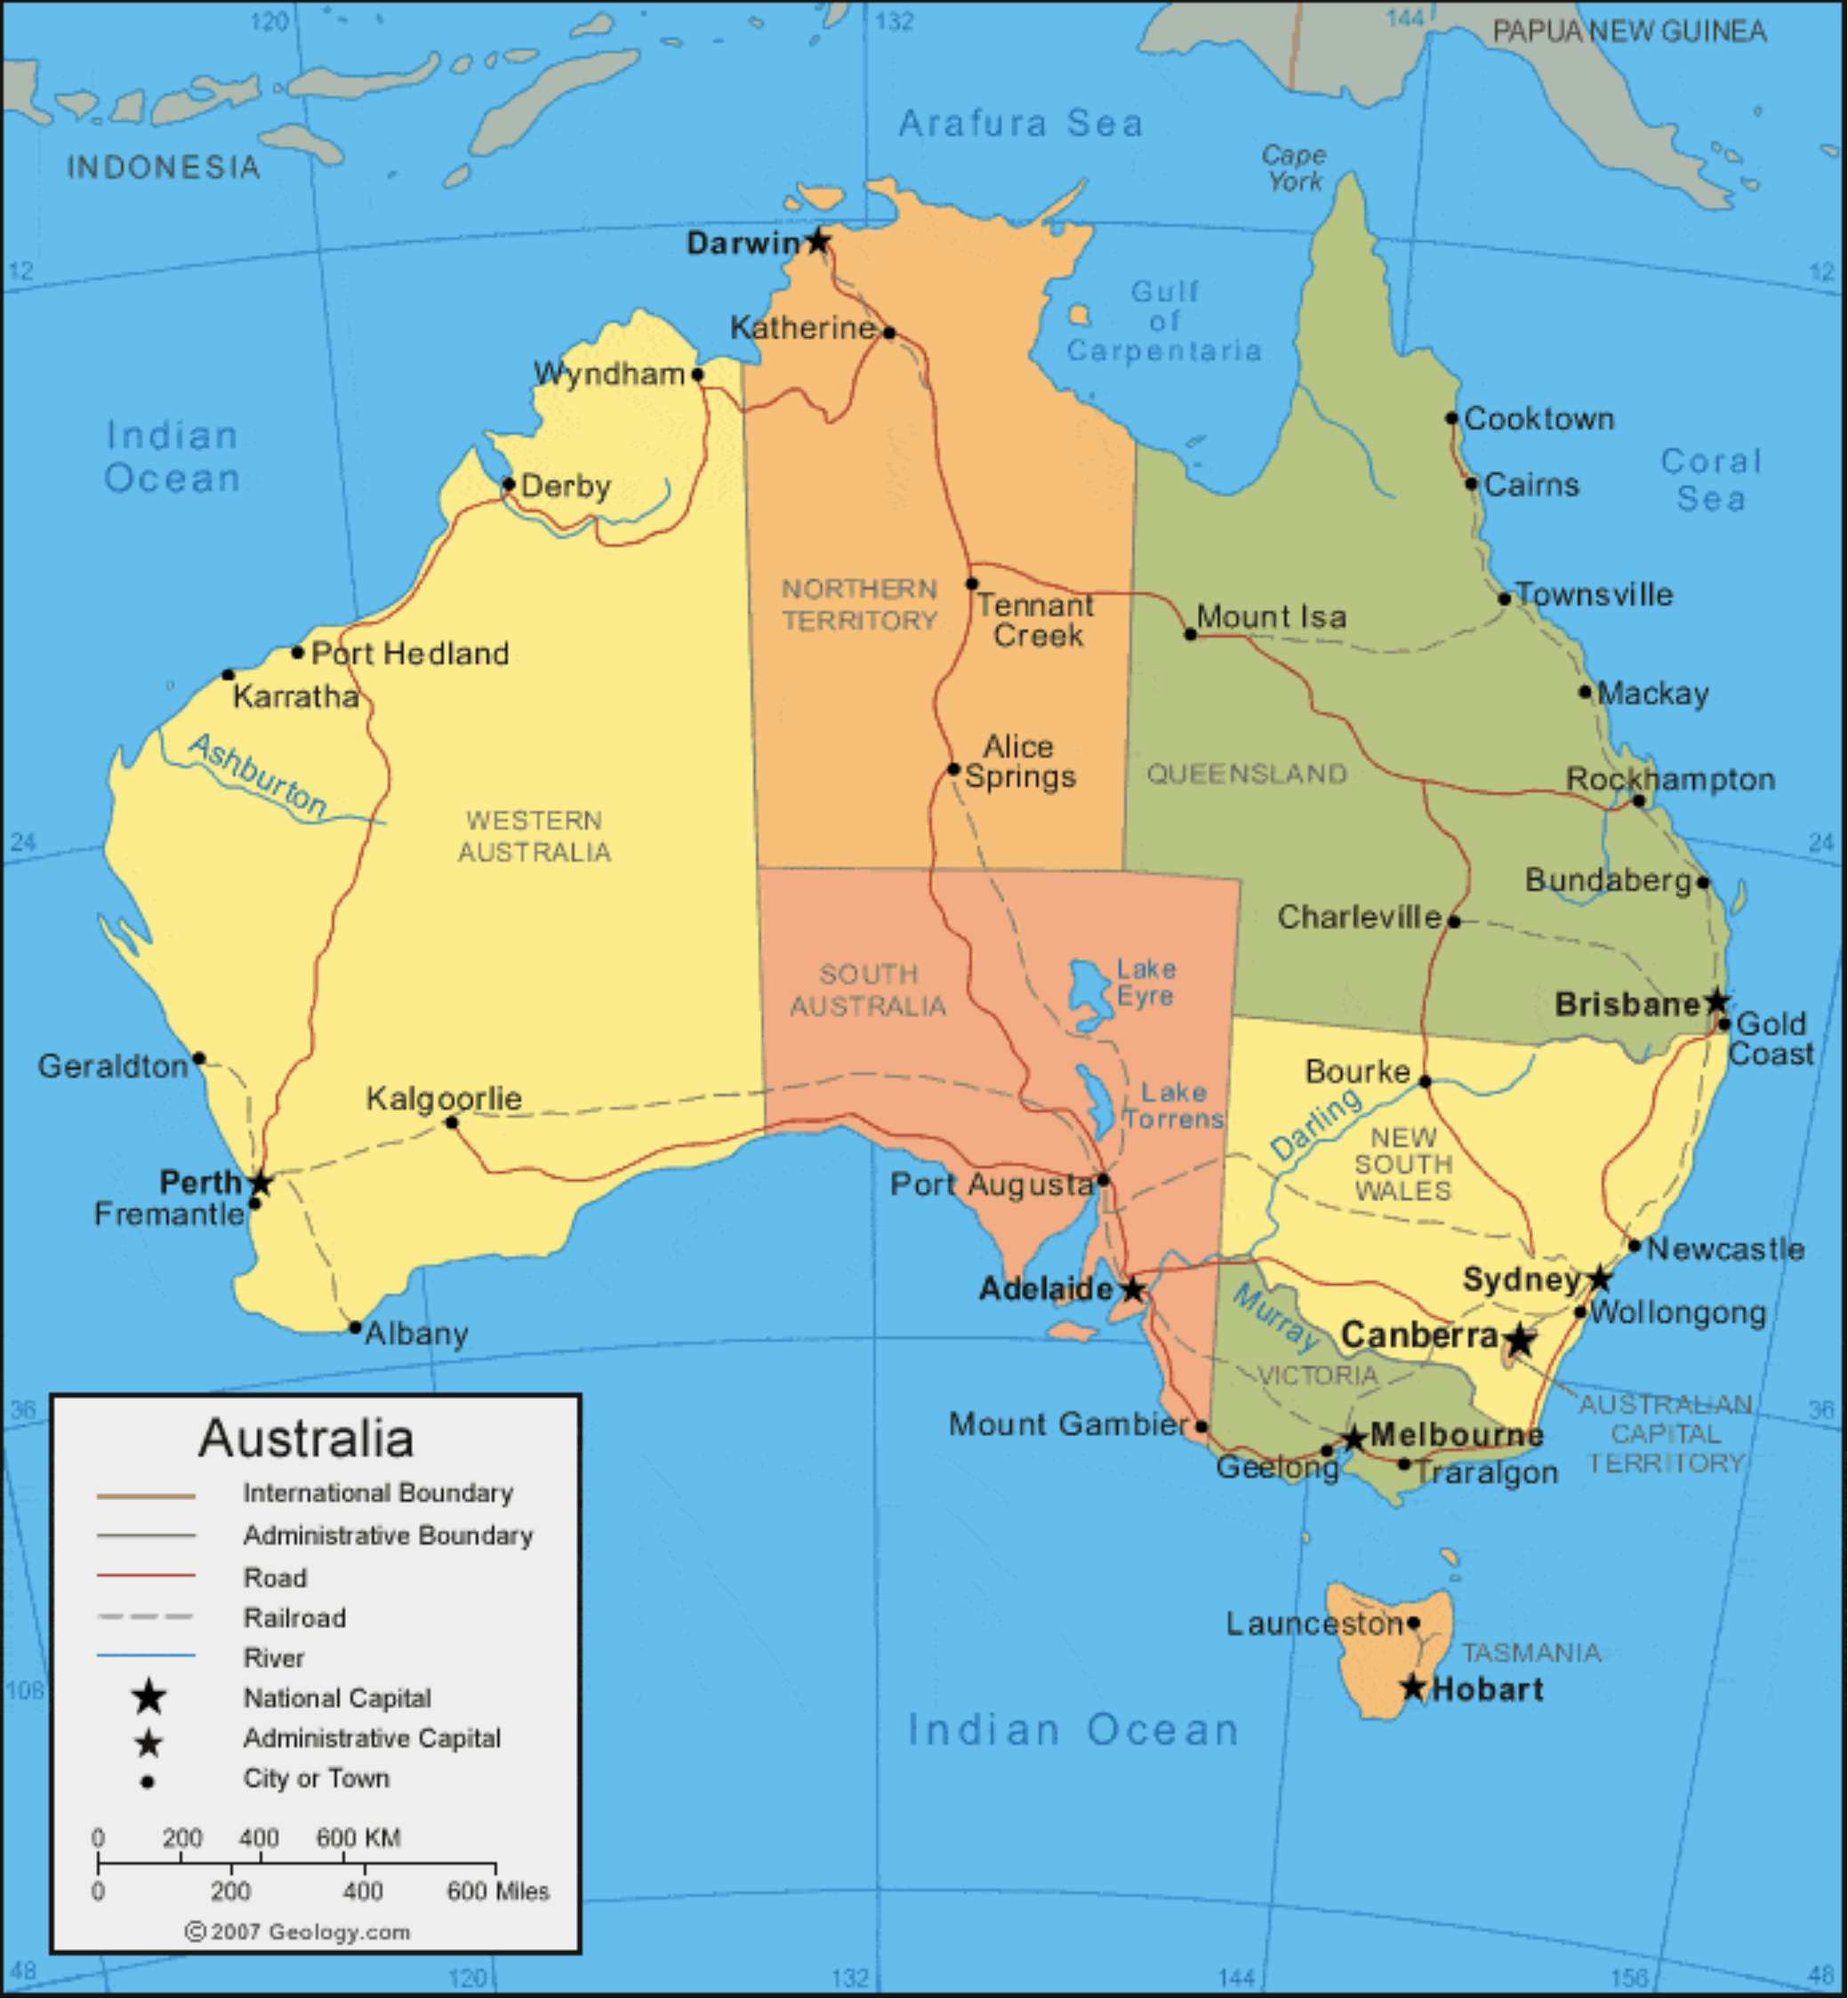
\epsfig{file=Figures/australia.pdf,scale=0.8}} 
  \caption{A map of Australia.}
  \label{fig:australia.pdf}
\end{figure}

\subsection{Example: Map Colouring}
In \href{https://en.wikipedia.org/wiki/Four_color_theorem}{map colouring} \index{map colouring} a map showing
different state 
borders is given and the task is to colour the different states such that no two states that have a common
border share the same colour.  \myFig{australia.pdf} shows a map of Australia.  There are seven different
states in Australia:
\begin{enumerate}
\item Western Australia, abbreviated as $\mathrm{WA}$,
\item Northern Territory, abbreviated as $\mathrm{NT}$,
\item South Australia, abbreviated as $\mathrm{SA}$,
\item Queensland, abbreviated as $\mathrm{Q}$,
\item New South Wales, abbreviated as $\mathrm{NSW}$,
\item Victoria, abbreviated as $\mathrm{V}$, and
\item Tasmania, abbreviated as $\mathrm{T}$.
\end{enumerate}
Figure \ref{fig:australia.pdf} would certainly look better if different states had been coloured with different
colours.  For the purpose of 
this example let us assume that we have only the three colours \red{red}, \green{green}, and \blue{blue} 
available.  The question then is whether it is  
possible to colour the different states in a way that no two neighbouring states share the same colour.  This
problem can be formalized as a constraint satisfaction problem.  To this end we define:
\begin{enumerate}
\item $\mytt{Vars} := \{ \mathtt{WA}, \mathtt{NT}, \mathtt{SA}, \mathtt{Q}, \mathtt{NSW}, \mathtt{V}, \mathtt{T} \}$,
\item $\mytt{Values} := \{ \mytt{red}, \mytt{green}, \mytt{blue} \}$,
\item $\mytt{Constraints} := $ \\[0.1cm]
      \hspace*{1.3cm}
      $\bigl\{ \mathtt{WA} \not= \mathtt{NT}, \mathtt{WA} \not= \mathtt{SA},
                 \mathtt{NT} \not= \mathtt{SA}, \mathtt{NT} \not= \mathtt{Q},
                 \mathtt{SA} \not= \mathtt{Q},  \mathtt{SA} \not= \mathtt{NSW}, \mathtt{SA} \not= \mathtt{V}, 
                 \mathtt{Q}  \not= \mathtt{NSW},
                 \mathtt{NSW}\not= \mathtt{V}
       \bigr\}
       $.
       \\[0.1cm]
       The constraints do not mention the variable \texttt{T} for Tasmania, as Tasmania does not share a common
       border with any of the other states.
\end{enumerate}
Then $\mathcal{P} := \langle \mytt{Vars}, \mytt{Values}, \mytt{Constraints} \rangle$ is a constraint satisfaction problem.  
If we define the assignment $\mathcal{I}$ such that
\begin{enumerate}
\item $\mathcal{I}(\mathtt{WA}) = \mytt{red}$,
\item $\mathcal{I}(\mathtt{NT}) = \mytt{blue}$,
\item $\mathcal{I}(\mathtt{SA}) = \mytt{green}$,
\item $\mathcal{I}(\mathtt{Q}) = \mytt{red}$,
\item $\mathcal{I}(\mathtt{NSW}) = \mytt{blue}$,
\item $\mathcal{I}(\mathtt{V}) = \mytt{red}$,
\item $\mathcal{I}(\mathtt{T}) = \mytt{green}$,
\end{enumerate}
then you can check that the assignment $\mathcal{I}$ is indeed a solution to the constraint satisfaction problem $\mathcal{P}$.
Figure \ref{fig:australia-solution.png} on page \pageref{fig:australia-solution.png} shows this solution.

\begin{figure}[!ht]
  \centering
  \framebox{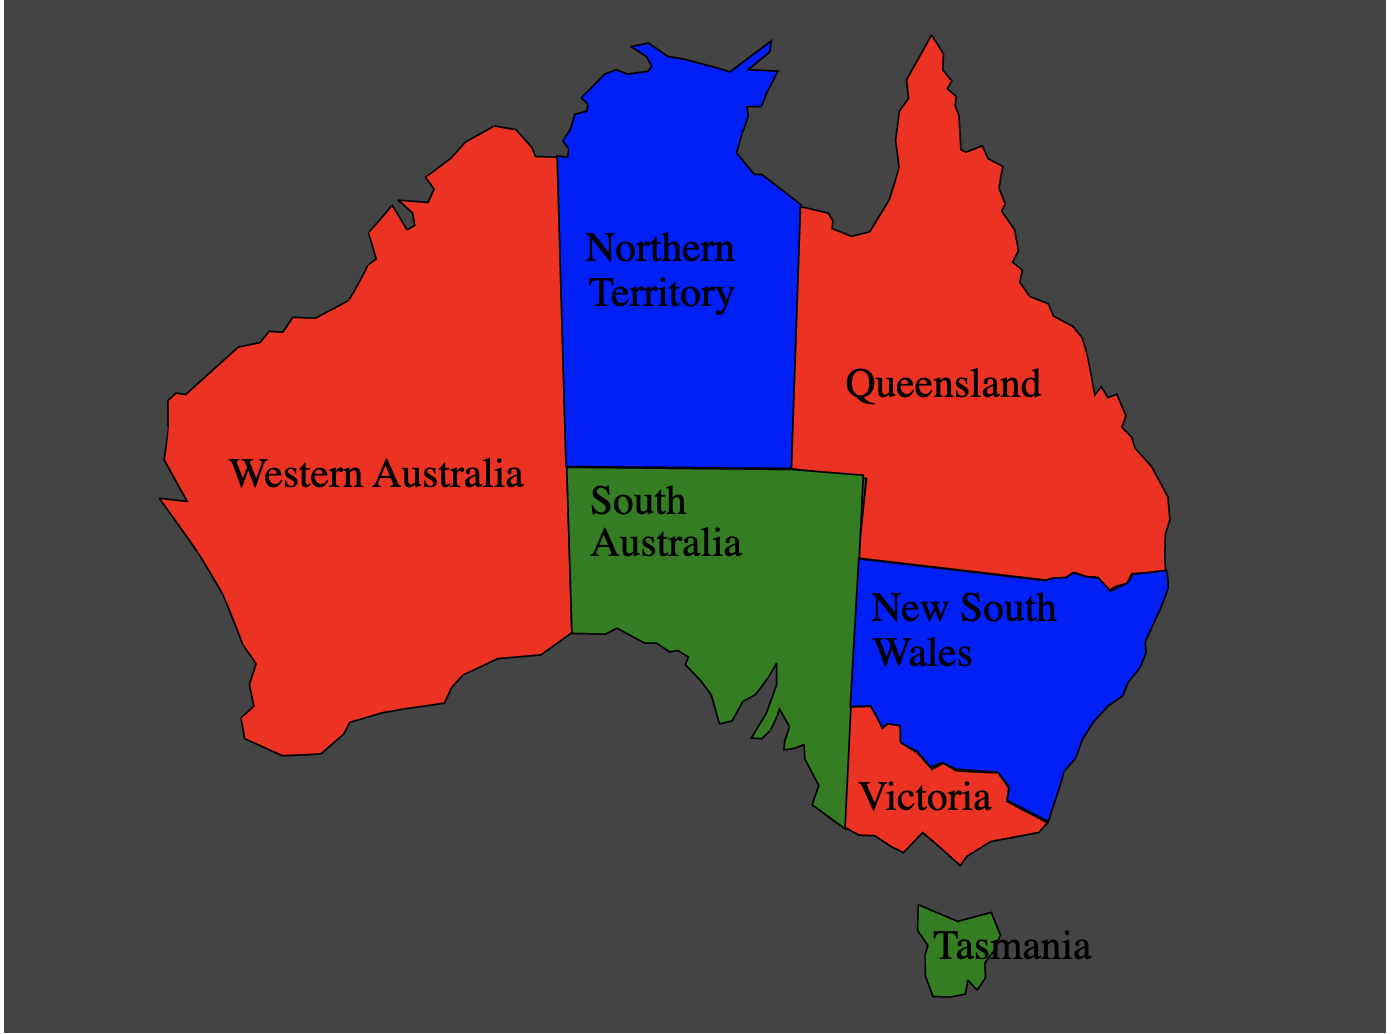
\epsfig{file=Figures/australia.png,scale=0.6}} 
  \caption{A map coloring for Australia.}
  \label{fig:australia-solution.png}
\end{figure}


\subsection{Example: The Eight Queens Puzzle}
\index{eight queens puzzle}
The \href{https://en.wikipedia.org/wiki/Eight_queens_puzzle}{eight queens problem} asks to put 8 queens onto a
chessboard such that no queen can attack another queen.  We have already discussed this problem in the previous
chapter.  Let us recapitulate: In \href{https://en.wikipedia.org/wiki/Chess}{chess},
a queen can attack all pieces that are either in the same row, the same column, or the same diagonal.  If we
want to put 8 queens on a chessboard such that no two queens can attack each other, we have to put exactly one
queen in every row:  If we would put more than one queen in a row, the queens in that row can attack each other.
If we would leave a row empty, then, given that the other rows contain at most one queen, there would be less
than 8 queens on the board.  Therefore, in order to model the eight queens problem as a constraint satisfaction
problem, we will use the following set of variables:
\\[0.2cm]
\hspace*{1.3cm}
$\mytt{Vars} := \{ \mytt{Q}_1, \mytt{Q}_2, \mytt{Q}_3, \mytt{Q}_4, \mytt{Q}_5, \mytt{Q}_6, \mytt{Q}_7,\mytt{Q}_8 \}$,
\\[0.2cm]
where for $i \in \{1,\cdots,8\}$ the variable $\mytt{Q}_i$ specifies the column of the queen that is placed in
row $i$.   As the columns run from one to eight, we define the set $\mytt{Values}$ as
\\[0.2cm]
\hspace*{1.3cm}
$\mytt{Values} := \{1,2,3,4,5,6,7,8\}$.
\\[0.2cm]
Next, let us define the constraints.  There are two different types of constraints.
\begin{enumerate}
\item We have constraints that express that no two queens positioned in different rows share the same column.
      To capture these constraints, we define
      \\[0.2cm]
      \hspace*{1.3cm}
      $\mytt{SameRow} := \bigl\{ \mytt{Q}_i \not= \mytt{Q}_j \bigm| i \in \{1,\cdots,8\} \wedge j \in \{1,\cdots,8\} \wedge j < i \bigr\}$.
      \\[0.2cm]
      Here the condition $i < j$ ensures that, for example, we have the constraint $\mytt{Q}_2 \not= \mytt{Q}_1$
      but not the constraint  $\mytt{Q}_1 \not= \mytt{Q}_2$, as the latter constraint would be redundant if
      the former constraint has already been established.
\item We have constraints that express that no two queens positioned in different rows share the same 
      diagonal.  The queens in row $i$ and row $j$ share the same diagonal iff the equation
      \\[0.2cm]
      \hspace*{1.3cm}
      $|i - j| = |\mytt{Q}_i - \mytt{Q}_j|$
      \\[0.2cm]
      holds.  The expression $|i-j|$ is the absolute value of the difference of the rows of the queens in row
      $i$ and row $j$,  while the expression $|\mytt{Q}_i - \mytt{Q}_j|$ is the absolute value of the difference of the
      columns of these queens.  To capture these constraints, we define
      \\[0.2cm]
      \hspace*{1.3cm}
      $\mytt{SameDiagonal} := \bigl\{ |i  - j| \not= |\mytt{Q}_i - \mytt{Q}_j| \bigm| i \in \{1,\cdots,8\} \wedge j \in \{1,\cdots,8\} \wedge j < i \bigr\}$.
\end{enumerate}
Then, the set of constraints is defined as 
\\[0.2cm]
\hspace*{1.3cm}
$\mytt{Constraints} := \mytt{SameRow} \cup \mytt{SameDiagonal}$
\\[0.2cm]
and the eight queens problem can be stated as the constraint satisfaction problem
\\[0.2cm]
\hspace*{1.3cm}
$\mathcal{P} := \langle \mytt{Vars}, \mytt{Values}, \mytt{Constraints} \rangle$.
\\[0.2cm]
If we define the assignment $\mathcal{I}$ such that
\\[0.2cm]
\hspace*{1.3cm}
$\mathcal{I}(\mytt{Q}_1) := 4,\; \mathcal{I}(\mytt{Q}_2) := 8,\; \mathcal{I}(\mytt{Q}_3) := 1,\;
\mathcal{I}(\mytt{Q}_4) := 2,\; \mathcal{I}(\mytt{Q}_5) := 6,\; \mathcal{I}(\mytt{Q}_6) := 2$,
\\[0.2cm]
\hspace*{1.3cm}
$\mathcal{I}(\mytt{Q}_7) := 7,\; \mathcal{I}(\mytt{Q}_8) := 5$,
\\[0.2cm]
then it is easy to see that this assignment is a solution of the eight queens problem.  This solution is shown
in \myFig{eight-queens.txt}.


\begin{figure}[!ht]
  \centering
\hspace*{0.0cm}
\vbox{\offinterlineskip
   \hrule height1pt
   \hbox{\vrule width1pt\bigchess
         \vbox{\hbox{0Z0L0Z0Z}
               \hbox{Z0Z0Z0ZQ}
               \hbox{QZ0Z0Z0Z}
               \hbox{Z0L0Z0Z0}
               \hbox{0Z0Z0L0Z}
               \hbox{ZQZ0Z0Z0}
               \hbox{0Z0Z0ZQZ}
               \hbox{Z0Z0L0Z0}}%
         \vrule width1pt}
   \hrule height1pt}

  \caption{A solution of the eight queens problem.}
  \label{fig:eight-queens.txt}
\end{figure}
Later, when we implement procedures to solve  \textsc{Csp}s, we will represent variable assignments and partial
variable assignments as dictionaries.  For example, the variable assignment $\mathcal{I}$ defined above would
then be represented as the dictionary 
\\[0.2cm]
\hspace*{1.3cm}
$\mathcal{I} = \bigl\{ \mytt{Q}_1:4,\, \mytt{Q}_2:8,\, \mytt{Q}_3:1,\, \mytt{Q}_4:3,\, 
             \mytt{Q}_5:6,\, \mytt{Q}_6:2,\, \mytt{Q}_7:7,\, \mytt{Q}_8:5) 
     \bigr\}$.
\\[0.2cm]
If we define 
\\[0.2cm]
\hspace*{1.3cm}
$\mathcal{B} := \bigl\{ \mytt{Q}_1:4,\, \mytt{Q}_2:8,\, \mytt{Q}_3:1) \bigr\}$,
\\[0.2cm]
then $\mathcal{B}$ is a partial assignment and $\mytt{dom}(\mathcal{B}) = \{ \mytt{Q}_1, \mytt{Q}_2, \mytt{Q}_3 \}$.  This
partial assignment is shown in \myFig{eight-queens-partial.txt}.

\begin{figure}[!ht]
  \centering
\hspace*{0.0cm}
\vbox{\offinterlineskip
   \hrule height1pt
   \hbox{\vrule width1pt\bigchess
         \vbox{\hbox{0Z0L0Z0Z}
               \hbox{Z0Z0Z0ZQ}
               \hbox{QZ0Z0Z0Z}
               \hbox{Z0Z0Z0Z0}
               \hbox{0Z0Z0Z0Z}
               \hbox{Z0Z0Z0Z0}
               \hbox{0Z0Z0Z0Z}
               \hbox{Z0Z0Z0Z0}}%
         \vrule width1pt}
   \hrule height1pt}

  \caption{The partial assignment $\bigl\{ \mytt{Q}_1 \mapsto 4, \mytt{Q}_2 \mapsto 8, \mytt{Q}_3 \mapsto 1) \bigr\}$.}
  \label{fig:eight-queens-partial.txt}
\end{figure}



\myFig{queens-csp.stlx} shows a \textsl{Python} program that can be used to create the eight queens puzzle as a
\textsc{Csp}.  

\begin{figure}[!ht]
\centering
\begin{minted}[ frame         = lines, 
                framesep      = 0.3cm, 
                firstnumber   = 1,
                bgcolor       = sepia,
                numbers       = left,
                numbersep     = -0.2cm,
                xleftmargin   = 0.2cm,
                xrightmargin  = 0.2cm,
              ]{python3}
    def queensCSP():
        'Returns a CSP coding the 8 queens problem.'
        S            = range(1, 8+1)          # used as indices
        Variables    = [ f'Q{i}' for i in S ]
        Values       = { 1, 2, 3, 4, 5, 6, 7, 8 }
        SameRow      = { f'Q{i} != Q{j}' for i in S for j in S if i < j }
        SameDiagonal = { f'abs(Q{i}-Q{j}) != {j-i}' for i in S for j in S if i < j }
        return (Variables, Values, SameRow | SameDiagonal)
\end{minted}
\vspace*{-0.3cm}
\caption{\textsl{Python} code to create the CSP representing the eight queens puzzle.}
\label{fig:queens-csp.stlx}
\end{figure}


\subsection{A Backtracking Constraint Solver}
One approach to solve a \textsc{Csp} that is both conceptually simple and reasonable efficient is
\blue{backtracking}.\index{backtracking}  The idea is to try to build variable assignments incrementally:  We start with
an empty dictionary and pick a variable $x_1$ that needs to have a value assigned.  For this variable, we
choose a value $v_1$ and assign it to this variable.  This yields the partial assignment $\{ x_1:v_1 \}$.
Next, we evaluate all those constraints that mention only the variable $x_1$ and check whether these constraints
are satisfied.  If any of these constraints is evaluated as \mytt{False}, we try to assign another value to
$x_1$ until we find a value that satisfies all constraints that mention only $x_1$.

In general, if we have a partial variable assignment $\mathcal{B}$ of the form
\\[0.2cm]
\hspace*{1.3cm}
$\mathcal{B} = \{ x_1:v_1, \cdots, x_k:v_k \}$
\\[0.2cm]
and we already know that all constraints that mention only the variables $x_1$, $\cdots$, $x_k$ are satisfied
by $\mathcal{B}$, then in order to extend $\mathcal{B}$ we pick another variable $x_{k+1}$ and choose a
value $v_{k+1}$ such that all those constraints that mention only the variables  $x_1$, $\cdots$, $x_k$,
$x_{k+1}$ are satisfied.  If we discover that there is no such value $v_{k+1}$, then we have to undo the
assignment $x_k:v_k$ and try to find a new value $v_k$ such that, first, those constraints mentioning only 
the variables  $x_1$, $\cdots$, $x_k$ are satisfied, and, second, it is possible to find a value $v_{k+1}$ that
can be assigned to $x_{k+1}$.  This step of going back and trying to find a new value for the variable $x_k$ is
called \blue{backtracking}.  It might be necessary to backtrack more than one level and to also undo the
assignment of $v_{k-1}$ to $x_{k-1}$ or, indeed, we might be forced to undo the assignments of all variables
$x_i$, $\cdots$, $x_k$ for some $i \in \{1,\cdots, n\}$.  The details of this search procedure are best
explained by looking at its implementation. \myFig{CSP-Solver.ipynb} shows a simple \textsc{Csp} solver that
employs backtracking.  We discuss this program next.

\begin{figure}[!ht]
\centering
\begin{minted}[ frame         = lines, 
                  framesep      = 0.3cm, 
                  firstnumber   = 1,
                  bgcolor       = sepia,
                  numbers       = left,
                  numbersep     = -0.2cm,
                  xleftmargin   = 0.8cm,
                  xrightmargin  = 0.8cm,
                  ]{python3}
    import ast
                  
    def collect_variables(expr): 
        tree = ast.parse(expr)
        return { node.id for node in ast.walk(tree) 
                         if  isinstance(node, ast.Name) 
                         if  node.id not in dir(__builtins__)
               }
                  
    def solve(CSP):
        'Compute a solution for the given constraint satisfaction problem.'
        Variables, Values, Constraints = CSP
        CSP = (Variables,
               Values,
               [(f, collect_variables(f) & set(Variables)) for f in Constraints]
              )
        return backtrack_search({}, CSP)
\end{minted}
\vspace*{-0.3cm}
\caption{A backtracking \textsc{Csp} solver}
\label{fig:CSP-Solver.ipynb}
\end{figure}

\begin{enumerate}
\item As we need to determine the variables occurring in a given constraint, we import the module
      \mytt{ast}.  This module implements the function $\mytt{parse}(e)$ that takes
      a \textsl{Python} expression $e$.  This expression is parsed and the resulting syntax tree is returned.
\item The function $\mytt{collect\_variables}(\mytt{expr})$ takes a \textsl{Python} expression as its input.
      It returns the set of variable names occurring in this expression.
\item The procedure $\mytt{solve}$ takes a constraint satisfaction problem $\mytt{CSP}$ as input and tries
      to find a solution.    
      \begin{enumerate}
      \item First, in line 11 the $\mytt{CSP}$ is split into its three components.  However, the first
            component $\mytt{Variables}$ does not have to be a set but rather can also be a list.
            If $\mytt{Variables}$ is a list, then backtracking search will assign these variables 
            in the same order as they appear in this list.  This can improve the efficiency of backtracking
            tremendously. 
      \item Next, for every constraint $\mytt{f}$ of the given $\mytt{CSP}$, we compute the set of variables that
            are used in $\mytt{f}$.  This is done using the procedure $\mytt{collect\_variables}$.
            Of these variables we keep only those variables that also occur in the set $\mytt{Variables}$
            because we assume that any other \textsl{Python} variable occurring in a constraint $f$ has already
            a value assigned to it and can therefore be regarded as a constant.

            The variables occurring in a constraint $\mytt{f}$ are then paired with the constraint $\mytt{f}$ and
            the correspondingly modified data structure is stored in $\mytt{CSP}$ and is called an
            \blue{augmented \textsc{Csp}}.

            The reason to compute and store these sets of variables is efficiency: When we later check whether
            a constraint $\mytt{f}$ is satisfied for a partial variable assignment $\mytt{Assignment}$ where $\mytt{Assignment}$ is
            stored as a dictionary, we only need to check the constraint $\mytt{f}$ iff all of the variables occurring
            in $\mytt{f}$ are elements of the domain of $\mytt{Assignment}$.   It would be wasteful to compute
            these sets of all variables occurring in a given formula every time the formula is checked.
      \item Next, we call the function $\mytt{backtrack\_search}$ to compute a solution of $\mytt{CSP}$.
   \end{enumerate}
 \end{enumerate}

 \begin{figure}[!ht]
\centering
\begin{minted}[ frame         = lines, 
                  framesep      = 0.3cm, 
                  firstnumber   = 1,
                  bgcolor       = sepia,
                  numbers       = left,
                  numbersep     = -0.2cm,
                  xleftmargin   = 0.0cm,
                  xrightmargin  = 0.0cm,
                ]{python3}          
def backtrack_search(Assignment, CSP):
    '''
    Given a partial variable assignment, this function tries to 
    complete this assignment towards a solution of the CSP.
    '''
    Variables, Values, Constraints = CSP
    if len(Assignment) == len(Variables): 
        return Assignment
    var = [x for x in Variables if x not in Assignment][0]
    for value in Values:
        if isConsistent(var, value, Assignment, Constraints):
            NewAssign      = Assignment.copy()
            NewAssign[var] = value
            Solution = backtrack_search(NewAssign, CSP)
            if Solution != None:
                return Solution
    return None 
\end{minted}
\vspace*{-0.3cm}
\caption{The function \mytt{backtrack\_search}}
\label{fig:CSP-Solver.ipynb-backtrack_search}
\end{figure}

Next, we discuss the implementation of the procedure $\mytt{backtrack\_search}$ that is shown in
\myFig{CSP-Solver.ipynb-backtrack_search}.  This procedure receives a partial assignment 
$\mytt{Assignment}$ as input together with an augmented $\mytt{CSP}$.  This partial assignment is
\blue{consistent} with $\mytt{CSP}$:  If $\mytt{f}$ is a constraint of $\mytt{CSP}$ such that
all the variables occurring in $\mytt{f}$ are assigned to in $\mytt{Assignment}$, then evaluating
$\mytt{f}$ using $\mytt{Assignment}$ yields $\mytt{True}$.  Initially, this partial assignment is empty
and hence trivially consistent.  The idea is to extend this partial assignment until it is a complete
assignment that satisfies all constraints of the given $\mytt{CSP}$.
\begin{enumerate}
\item First, the augmented $\mytt{CSP}$ is split into its components.
\item Next, if $\mytt{Assignment}$ is already a complete variable assignment, i.e.~if the dictionary
      $\mytt{Assignment}$ has as many elements as there are variables, then the fact that
      $\mytt{Assignment}$ is partially consistent implies that
      it is a solution of the $\mytt{CSP}$ and, therefore, it is returned.
\item Otherwise, we have to extend the partial $\mytt{Assignment}$.  In order to do so, we first have to
      select a variable $\mytt{var}$ that has not yet been assigned a value in $\mytt{Assignment}$ so far.
      We pick the first variable in the list \mytt{Variables} that is yet unassigned.
      This variable is called $\mytt{var}$.
\item Next, we try to assign a $\mytt{value}$ to the selected variable $\mytt{var}$.  After assigning
      a $\mytt{value}$ to $\mytt{var}$, we immediately check whether this assignment would be consistent
      with the constraints using the procedure $\mytt{isConsistent}$.
      If the partial $\mytt{Assignment}$ turns out to be consistent, the partial $\mytt{Assignment}$
      is extended to the new partial assignment \mytt{NewAssign} that satisfies
      \\[0.2cm]
      \hspace*{1.3cm}
      \mytt{NewAssign[var] = value}
      \\[0.2cm]
      and that coincides with $\mytt{Assignment}$ for all variables different from $\mytt{var}$.
      Then, the procedure $\mytt{backtrack\_search}$ is called recursively to complete this new partial assignment.
      If this is successful, the resulting assignment is a solution of the CSP and is returned.  Otherwise the
      \texttt{for}-loop in line 10 tries the next $\mytt{value}$.
      If all possible values have been tried and none was successful, the \texttt{for}-loop
      ends and the function returns $\mytt{None}$.
\end{enumerate}


\begin{figure}[!ht]
\centering
\begin{minted}[ frame         = lines, 
                framesep      = 0.3cm, 
                firstnumber   = 1,
                bgcolor       = sepia,
                numbers       = left,
                numbersep     = -0.2cm,
                xleftmargin   = 0.0cm,
                xrightmargin  = 0.0cm,
              ]{python3}  
    def isConsistent(var, value, Assignment, Constraints):
        NewAssign      = Assignment.copy()
        NewAssign[var] = value
        return all(eval(f, NewAssign) for (f, Vs) in Constraints
                                      if var in Vs and Vs <= NewAssign.keys()
                  )
\end{minted}
\vspace*{-0.3cm}
\caption{The procedure \mytt{isConsistent}}
\label{fig:CSP-Solver.ipynb-isConsistent}
\end{figure}

We still need to discuss the implementation of the auxiliary procedure $\mytt{isConsistent}$
shown in \myFig{CSP-Solver.ipynb-isConsistent}.  This procedure takes a variable $\mytt{var}$, a $\mytt{value}$, a partial 
$\mytt{Assignment}$ and a set of $\mytt{Constraints}$.  It is assumed that $\mytt{Assignment}$ is
\blue{partially consistent} with respect to the set $\mytt{Constraints}$, i.e.~for every formula $\mytt{f}$
occurring in $\mytt{Constraints}$ such that
\\[0.2cm]
\hspace*{1.3cm}
$\mytt{vars}(\mytt{f}) \subseteq \mytt{dom}(\mytt{Assignment})$
\\[0.2cm]
holds, the formula $\mytt{f}$ evaluates to $\mytt{True}$ given the $\mytt{Assignment}$.  The purpose of
$\mytt{isConsistent}$ is to check, whether the extended assignment
\\[0.2cm]
\hspace*{1.3cm}
$\mytt{NA} \;\mytt{:=}\;\mytt{Assignment} \cup \{ \pair(\mytt{var}, \mytt{value}) \}$
\\[0.2cm]
that assigns $\mytt{value}$ to the variable $\mytt{var}$ is still partially consistent with $\mytt{Constraints}$. 
To this end, the \mytt{for}-loop iterates over all $\mytt{Formula}$s in $\mytt{Constraints}$. 
However, we only have to check those $\mytt{Formula}$s that contain the variable $\mytt{var}$ and,
furthermore, have the property that
\\[0.2cm]
\hspace*{1.3cm}
$\mytt{Vars}(\mytt{Formula}) \subseteq \mytt{dom}(\mytt{NA})$,
\\[0.2cm]
i.e.~all variables occurring in $\mytt{Formula}$ need to have a value assigned in
$\mytt{NA}$.  The reasoning is as follows:
\begin{enumerate}
\item If $\mytt{var}$ does not occur in $\mytt{Formula}$, then adding $\mytt{var}$ to
      $\mytt{Assignment}$ cannot change the result of evaluating $\mytt{Formula}$ and as
      $\mytt{Assignment}$ is assumed to be partially consistent with respect to $\mytt{Formula}$, 
      $\mytt{NA}$ is also partially consistent with respect to $\mytt{Formula}$.
\item If $\mytt{dom}(\mytt{NA}) \not\subseteq \mytt{Vars}(\mytt{Formula})$, then $\mytt{Formula}$ can not be evaluated anyway. 
\end{enumerate}
If we use backtracking, we can solve the 8 queens problem in less than a second.
For the eight queens puzzle the order in which variables are tried is not particularly important.  The reason
is that all variables are connected to all other variables.  For other problems the ordering of the variables
can be \red{very important}.  The general strategy is that variables that are strongly related to each other should
be grouped together in the list $\mytt{Variables}$.

\section{Solving Search Problems by Constraint Programming}
In this section we show how we can formulate certain \blue{search problems} as \mytt{CSP}s.
We will explain our method by solving the
\href{https://en.wikipedia.org/wiki/Missionaries_and_cannibals_problem}{missionaries and cannibals problem},
which is explained in the following:
Three missionaries and three infidels have to cross a river in order to get to a church where the infidels can
be baptized.  According to ancient catholic mythology, baptizing the infidels is necessary to save them from
the eternal tortures of hell fire. In order to cross the river, the missionaries and infidels have a small boat
available that can take at most two passengers. If at any moments at any shore there are more infidels than
missionaries, then the missionaries have a problem, since the infidels have a diet that is rather unhealthy for
the missionaries. 

In order to solve this problem via constraint programming, we first introduce the notion of a
\blue{symbolic transition system}.

\begin{Definition}[Symbolic Transition System]
  A symbolic transition system is a 6-tuple
  \\[0.2cm]
  \hspace*{1.3cm}
  $\mathcal{T} = \langle \mathtt{Vars}, \mathtt{Values}, \mathtt{Start}, \mathtt{Goal}, \mathtt{Invariant}, \mathtt{Transition} \rangle$
  \\[0.2cm]
  such that:
  \begin{enumerate}[(a)]
  \item \texttt{Vars} is a set of variables.

        These variables are strings.  For every variable $x \in \texttt{Vars}$ there is a \blue{primed}
        variable $x'$ which does not occur in \texttt{Vars}.  The set of these primed Variables is denoted as
        $\mathtt{Vars}'$.
  \item \texttt{Values} is a set of values that these variables can take.
  \item \texttt{Start}, \texttt{Goal}, and \texttt{Invariant} are \textsc{Fol} formulas such that all free
         variables occurring in these formulas are elements from the set \texttt{Vars}.
         \begin{itemize}
         \item \texttt{Start} describes the initial state of the transition system.
         \item \texttt{Goal} describes a state that should be reached by the transition system.
         \item \texttt{Invariant} is a formula that has to be true for every state of the transition system.
         \end{itemize}
  \item \texttt{Transition} is a \textsc{Fol} formula.  The free variables of this formula are elements of
        the set $\texttt{Vars} \cup \mathtt{Vars}'$, i.e.~they are either variables from the set \texttt{Vars}
        or they are primed variables from the set $\mathtt{Vars}'$.

        The formula \texttt{Transition} describes how the variables in the transition system change during a
        state transition.  The primed variables refer to the values of the original variables after the
        state transition.
  \end{enumerate}
\end{Definition}
Every \blue{state} of a transition system is a mapping of the variable to values.
The idea is that the formula \texttt{Start} describes the start state of our search problem, \texttt{Goal}
describes the state that we want to reach, while \texttt{Invariant} is a formula that must be true initially
and that has to remain true after every transition of our system.


In order to clarify this definition we show how the \emph{missionaries and cannibals} problem can be formulated as
a symbolic transition system.
\begin{enumerate}[(a)]
\item $\texttt{Vars} := \{ \mathtt{M}, \mathtt{C}, \mathtt{B} \}$.

      \texttt{M} is the number of missionaries on the western shore, \texttt{C} is the number of infidels on
      that shore, while \texttt{B} is the number of boats.
\item $\mathtt{Values} := \{ 0, 1, 2, 3 \}$.
\item $\texttt{Start} := (\mathtt{M} = 3 \wedge \mathtt{C} = 3 \wedge \mathtt{B} = 1)$.
\item $\texttt{Goal}  := (\mathtt{M} = 0 \wedge \mathtt{C} = 0 \wedge B = 0)$.
\item $\texttt{Invariant} := \bigl((\mathtt{M} = 3 \vee \mathtt{M} = 0 \vee \mathtt{M} = C) \;\wedge\; \mathtt{B} \leq 1\bigr)$,

      since there is no problem when all missionaries are either on the western shore or on the eastern shore
      or when the number of missionaries is the same as the number of infidels on the western shore, because
      then these numbers have to agree on the eastern shore as well.

      Furthermore, there is just one boat.
\item $\texttt{Transition} :=
      \begin{array}[t]{cl}
         &  \mathtt{B}' = 1 - \mathtt{B}   \\[0.2cm]
        \wedge & \bigl(\mathtt{B} = 1 \;\rightarrow\; 1 \leq \mathtt{M} - \mathtt{M}'  + \mathtt{C} - \mathtt{C}' \leq 2 \;\wedge\;
        \mathtt{M}' \leq \mathtt{M} \;\wedge\; \mathtt{C}' \leq \mathtt{C}\bigr) \\[0.2cm]
        \wedge & \bigl(\mathtt{B} = 0 \;\rightarrow\; 1 \leq \mathtt{M}' - \mathtt{M}  + \mathtt{C}' - \mathtt{C} \leq 2 \;\wedge\;
                \mathtt{M}' \geq \mathtt{M} \;\wedge\; \mathtt{C}' \geq \mathtt{C}\bigr) 
      \end{array}
      $

      Let us explain the details of this formula:
      \begin{itemize}
      \item $\mathtt{B}' = 1 - \mathtt{B}$

            If the boat is initially on the western shore, i.e. $\texttt{B} = 1$, it will be on the eastern
            shore afterwards, i.e. we will then have $\texttt{B}' = 0$.  If, instead, the boat is initially on
            the eastern shore, i.e. $\texttt{B} = 0$, it will be on the western
            shore afterwards and then we have $\texttt{B}' = 1$.
      \item $\mathtt{B} = 1 \;\rightarrow\; 1 \leq \mathtt{M} - \mathtt{M}'  + \mathtt{C} - \mathtt{C}' \leq 2 \;\wedge\;
             \mathtt{M}' \leq \mathtt{M} \;\wedge\; \mathtt{C}' \leq \mathtt{C}$


            If the boat is initially on the western shore, then afterwards the number of missionaries and
            infidels will decrease, as they leave for the eastern shore.  In this case $\texttt{M} - \texttt{M}'$
            is the number of missionaries on the boat, while $\texttt{C} - \texttt{C}'$ is the number of
            infidels.  The sum of these numbers has to be between $1$ and $2$ because the boat can not travel
            empty and can take at most two passengers.
            
      \item $\mathtt{B} = 0 \;\rightarrow\; 1 \leq \mathtt{M}' - \mathtt{M}  + \mathtt{C}' - \mathtt{C} \leq 2 \;\wedge\;
            \mathtt{M}' \geq \mathtt{M} \;\wedge\; \mathtt{C}' \geq \mathtt{C}$

            This formula describes the transition from the eastern shore to the western shore and is analogous
            to the previous formula.
      \end{itemize}
\end{enumerate}

\begin{figure}[!ht]
\centering
\begin{Verbatim}[frame         = lines, 
                 framesep      = 0.3cm, 
                 firstnumber   = 1,
                 numbers       = left,
                 numbersep     = -0.2cm,
                 xleftmargin   = 0.8cm,
                 xrightmargin  = 0.8cm,
                 commandchars  = \\\{\},
                 codes         = {\catcode`$=3\catcode`^=7}
               ] 
    def start(M, C, B):
        return M == 3 and C == 3 and B == 1
    
    def goal(M, C, B):
        return M == 0 and C == 0 and B == 0
    
    def invariant(M, C, B):
        return (M == 0 or M == 3 or M == C) and B <= 1
    
    def transition(M$\alpha$, C$\alpha$, B$\alpha$, M$\beta$, C$\beta$, B$\beta$):
        if not (B$\beta$ == 1 - B$\alpha$):
            return False
        if B$\alpha$ == 1:
            return 1 <= M$\alpha$ - M$\beta$ + C$\alpha$ - C$\beta$ <= 2 and M$\beta$ <= M$\alpha$ and C$\beta$ <= C$\alpha$
        else:
            return 1 <= M$\beta$ - M$\alpha$ + C$\beta$ - C$\alpha$ <= 2 and M$\beta$ >= M$\alpha$ and C$\beta$ >= C$\alpha$
\end{Verbatim}
\vspace*{-0.3cm}
\caption{Coding the \emph{missionaries and cannibals problem} as a symbolic transition system.}
\label{fig:Missionaries-STS.ipynb}
\end{figure}

%$
Figure \ref{fig:Missionaries-STS.ipynb} shows how the \emph{missionaries and cannibals problem} can be
represented as a symbolic transition system in \textsl{Python}.  In the function \texttt{transition} 
we use the following convention: Since variables cannot be primed in
\textsl{Python} we append the character $\alpha$ to the names of the original
variables from the set \texttt{Vars}, while we append $\beta$ to these names to get the primed versions of the
corresponding variable.


\begin{figure}[!ht]
\centering
\begin{minted}[ frame         = lines, 
                framesep      = 0.3cm, 
                firstnumber   = 1,
                bgcolor       = sepia,
                numbers       = left,
                numbersep     = -0.2cm,
                xleftmargin   = 0.0cm,
                xrightmargin  = 0.0cm,
              ]{python3}
    def flatten(LoL):
        return [x for L in LoL for x in L]
                    
    def missionaries_CSP(n):
        "Returns a CSP encoding the problem."
        Lists        = [[f'M{i}', f'C{i}', f'B{i}'] for i in range(n+1)]
        Variables    = flatten(Lists)
        Values       = { 0, 1, 2, 3 }
        Constraints  = {  'start(M0, C0, B0)'      }  # start state
        Constraints |= { f'goal(M{n}, C{n}, B{n})' }  # goal state
        for i in range(n):
            Constraints.add(f'invariant(M{i}, C{i}, B{i})')
            Constraints.add(f'transition(M{i}, C{i}, B{i}, M{i+1}, C{i+1}, B{i+1})')
        return Variables, Values, Constraints
        
    def find_solution():
        n = 1
        while True:
            print(n)
            CSP = missionaries_CSP(n)
            Solution = solve(CSP)
            if Solution != None:
                return n, Solution
            n += 2
\end{minted}
\vspace*{-0.3cm}
\caption{Turning the symbolic transition system into a \textsc{Csp}.}
\label{fig:Missionaries-STS.ipynb-2}
\end{figure}

Figure \ref{fig:Missionaries-STS.ipynb-2} shows how we can turn the symbolic transition system into a
\textsc{Csp}.
\begin{enumerate}
\item The function $\texttt{flatten}(\texttt{LoL})$ receives a list $\texttt{LoL}$ of lists as its argument.
       This list has the form
       \\[0.2cm]
       \hspace*{1.3cm}
       $\texttt{LoL} = [L_1, \cdots, L_k]$
       \\[0.2cm]
       where the $L_i$ are lists for $i=1,\cdots,k$.
       
       It returns the list
       \\[0.2cm]
       \hspace*{1.3cm}
       $L_1 + \cdots + L_k$,
       \\[0.2cm]
       i.e.~it appends these lists and returns the result.
\item The function $\mathtt{missionaries\_CSP}(n)$ receives a natural number $n$ as its argument.
       It returns a \textsc{Csp} that has a solution if there is a solution of the \emph{missionaries and cannibals}
       problem that crosses the river exactly $n$ times.  It uses the variables
       \\[0.2cm]
       \hspace*{1.3cm}
       $\mathtt{M}_i$, $\mathtt{C}_i$, and $\mathtt{B}_i$, where $i=0,\cdots,n$.
       \\[0.2cm]
       $\mathtt{M}_i$ is the number of missionaries on the western shore after the boat has crossed the river
       $i$ times. The variables $\mathtt{C}_i$ and $\texttt{B}_i$ denote the number of infidels and boats
       respectively.

       Line 12 ensures that the invariant of the transition system is valid after every crossing of the boat.
       Line 13 describes the mechanics of the crossing.
\item The function \texttt{find\_solution} tries to find a natural number $n$ such that problem can be solved
       with $n$ crossings. As the number off crossings has to be odd, we increment $n$ by two.
\end{enumerate}


\section{Z3}
We conclude this chapter with a discussion of the solver
\href{https://www.microsoft.com/en-us/research/project/z3-3/}{Z3}.  
Z3 implements most of the state-of-the-art constraint solving algorithms and is exceptionally powerful.  We
introduce Z3 via a series of examples.

\subsection{A Simple Text Problem}
The following is a simple text problem from my old $8^{\textrm{th}}$ grade math book.
\textsl{
  \begin{itemize}
  \item I have as many brothers as I have sisters.
  \item My sister has twice as many brothers as she has sisters.
  \item How many children does my father have?
  \end{itemize}}
\noindent
However, in order to solve this puzzle we need two additional assumptions.
\begin{enumerate}
\item My father has no illegitimate children.
\item All of my fathers children identify themselves as either male or female.
\end{enumerate}
Strangely, in my old math book these assumptions are not mentioned.

We can now infer the number of children.
If we denote the number of \blue{boys} with the variable $b$ and the number of \blue{girls} with
$g$, the problem statements are equivalent to the following two equations:
\begin{enumerate}[(a)]
\item $b - 1 = g$.
\item $2 \cdot (g - 1) = b$.
\end{enumerate}
Before we can start to solve this problem, we have to install \texttt{Z3} via \texttt{pip} using the following
command:  
\\[0.2cm]
\hspace*{1.3cm}
\texttt{pip install z3-solver}


\begin{figure}[!ht]
\centering
\begin{minted}[ frame         = lines, 
                 framesep      = 0.3cm, 
                 firstnumber   = 1,
                 bgcolor       = sepia,
                 numbers       = left,
                 numbersep     = -0.2cm,
                 xleftmargin   = 0.8cm,
                 xrightmargin  = 0.8cm,
               ]{python3}             
    import z3
    
    boys  = z3.Int('boys')
    girls = z3.Int('girls')
    
    S = z3.Solver()
    
    S.add(boys - 1 == girls)
    S.add(2 * (girls - 1) == boys)
    S.check()
    Solution = S.model()
    
    b = Solution[boys ].as_long()
    g = Solution[girls].as_long()
    
    print(f'My father has {b + g} children.')
\end{minted}
\vspace*{-0.3cm}
\caption{Solving a simple text problem.}
\label{fig:Brothers-and-Sisters.ipynb}
\end{figure}

\noindent
Figure \ref{fig:Brothers-and-Sisters.ipynb} on page \pageref{fig:Brothers-and-Sisters.ipynb} shows how we can
solve the given problem using the \textsl{Python}
interface of Z3.
\begin{enumerate}
\item In line 1 we import the module \texttt{z3} so that we can use the Python \textsc{Api} of Z3.
      The documentation of this \textsc{Api} is available at the following address:
      \\[0.2cm]
      \hspace*{1.3cm}
      \href{https://ericpony.github.io/z3py-tutorial/guide-examples.htm}{https://ericpony.github.io/z3py-tutorial/guide-examples.htm}
\item Lines 3 and 4 creates the \texttt{Z3} variables \mytt{boys} and \mytt{girls} as integer valued variables.
      The function \mytt{Int} takes one argument, which has to be a string.  This string is the name of the
      variable.  We store these variables in Python variables of the same name.  It would be possible to use
      different names for the Python variables, but that would be very confusing.
\item Line 6 creates an object of the class \texttt{Solver}.  This is the constraint solver provided by
      \texttt{Z3}.
\item Lines 8 and 9 add the constraints expressing that the number of girls is one less than the number of boys
      and that my sister has twice as many brothers as she has sisters as constraints to the solver
      \texttt{S}.
\item In line 10 the method \mytt{check} examines whether the given set of constraints is satisfiable.
      In general, this method returns one of the following results:
      \begin{enumerate}[(a)]
      \item \mytt{sat} is returned if the problem is solvable, (\mytt{sat} is short for \emph{satisfiable})
      \item \mytt{unsat} is returned if the problem is unsolvable,
      \item \mytt{unknown} is returned if \texttt{Z3} is not powerful enough to solve the given problem.
      \end{enumerate}
\item Since in our case the method \mytt{check} returns \texttt{sat}, we can extract the solution that is
      computed via the method \mytt{model} in line 11.  
\item In order to extract the values that have been computed by \texttt{Z3} for the variables \mytt{boys} and
      \mytt{girls}, we can use dictionary syntax and write \mytt{Solution[boys]} and
      \mytt{Solution[girls]} to extract these values.  However, these values are not stored as integers but
      rather as objects of the class \mytt{IntNumRef}, which is some internal class of \texttt{Z3} to store
      integers.  This class provides the method \mytt{as\_long} that converts its argument into an integer number.
\end{enumerate}
\pagebreak

\exerciseEng
Solve the following text problem using \texttt{Z3}.
\textsl{
  \begin{enumerate}[(a)]
  \item A Japanese deli offers both
        \href{https://www.discovermagazine.com/health/hearty-penguin-steaks-the-old-school-explorers-salve-for-scurvy}{penguins}
        and \href{http://fancytoast.blogspot.com/2007/04/parrot-three-ways.html}{parrots}.  
  \item A parrot and a penguin together cost 666 bucks.
  \item The penguin costs 600 bucks more than the parrot.  
  \end{enumerate}}
  \noindent
  \textbf{What is the price of the parrot?} You may assume that the prizes of these delicacies are integer valued. 
\eox

\exerciseEng
Solve the following text problem using \texttt{Z3}.
\textsl{
  \begin{enumerate}[(a)]
  \item  A train travels at a uniform speed for 360 miles.  
  \item  The train would have taken 48 minutes less to travel the same distance 
         if it had been faster by 5 miles per hour.
  \end{enumerate}}
\noindent
\textbf{Find the speed of the train!}

\noindent
\textbf{Hints:}
\begin{enumerate}[(a)]
\item As the speed is a real number you should declare this variable via the \texttt{Z3} function \texttt{Real} instead of using
      the function \texttt{Int}.
\item Be careful to not mix up different units. In particular, the time 48 minutes should be expressed as a
      fraction of an hour.
\item When you formulate the information given above, you will get a system of \textbf{non-linear} equations,
      which is equivalent to a quadratic equation.  This quadratic equation has two different solutions.
      One of these solutions is negative.  In order to exclude the negative solution you need to add a
      constraint stating that the speed of the train has to be greater than zero.
\end{enumerate}

\subsection{The Knight's Tour}
In this subsection we will solve the puzzle \href{https://en.wikipedia.org/wiki/Knight%27s_tour}{The Knight's Tour} 
using \texttt{Z3}.  This puzzle asks whether it is possible for a knight to visit all 64 squares of a chess board
in 63 moves.  We will start the tour in the upper left corner of the board.  

In order to model this puzzle as a constraint satisfaction problem we first have to decide on the variables
that we want to use. The idea is to have 64 variables that describe the position of the knight after its
$i^{\mathrm{th}}$ move where $i=0,1,\cdots,63$.  However, it turns out that it is best to split the values of these positions up into a
row and a column.  If we do this, we end up with 128 variables of the form
\\[0.2cm]
\hspace*{1.3cm}
$\mathtt{R}_i$ and $\mathtt{C}_i$ \quad for $i \in \{0, 1, \cdots, 63\}$.
\\[0.2cm]
Here $\mathtt{R}_i$ denotes the row of the knight after its $i^{\mathrm{th}}$ move, while $\mathtt{C}_i$
denotes the corresponding column.  
Next, we have to formulate the constraints.  In this case, there are two kinds of constraints:
\begin{enumerate}
\item We have to specify that the move from the position $\langle \mathtt{R}_i, \mathtt{C}_i \rangle$
      to the position $\langle \mathtt{R}_{i+1}, \mathtt{C}_{i+1} \rangle$ is legal move for a knight.
      In chess, there are two ways for a knight to move:
      \begin{enumerate}[(a)]
      \item The knight can move two squares horizontally left or right followed by moving vertically
            one square up or down, or
      \item the knight can move two squares vertically up or down followed by moving
            one square left or right.
      \end{enumerate}
      Figure \ref{fig:knight-moves.png} shows all legal moves of a knight that is positioned in the square \texttt{e4}.
      Therefore, a formula that expresses that the $i^{\mathrm{th}}$ move is a legal move of the knight is a disjunction
      of the following eight formulas that each describe one possible way for the knight to move:
      \begin{enumerate}
      \item $\mathtt{R}_{i+1} = \mathtt{R}_{i} + 2 \;\wedge\; \mathtt{C}_{i+1} = \mathtt{C}_{i} + 1$,
      \item $\mathtt{R}_{i+1} = \mathtt{R}_{i} + 2 \;\wedge\; \mathtt{C}_{i+1} = \mathtt{C}_{i} - 1$, 
      \item $\mathtt{R}_{i+1} = \mathtt{R}_{i} - 2 \;\wedge\; \mathtt{C}_{i+1} = \mathtt{C}_{i} + 1$, 
      \item $\mathtt{R}_{i+1} = \mathtt{R}_{i} - 2 \;\wedge\; \mathtt{C}_{i+1} = \mathtt{C}_{i} - 1$, 
      \item $\mathtt{R}_{i+1} = \mathtt{R}_{i} + 1 \;\wedge\; \mathtt{C}_{i+1} = \mathtt{C}_{i} + 2$, 
      \item $\mathtt{R}_{i+1} = \mathtt{R}_{i} + 1 \;\wedge\; \mathtt{C}_{i+1} = \mathtt{C}_{i} - 2$, 
      \item $\mathtt{R}_{i+1} = \mathtt{R}_{i} - 1 \;\wedge\; \mathtt{C}_{i+1} = \mathtt{C}_{i} + 2$, 
      \item $\mathtt{R}_{i+1} = \mathtt{R}_{i} - 1 \;\wedge\; \mathtt{C}_{i+1} = \mathtt{C}_{i} - 2$. 
      \end{enumerate}
\item Furthermore, we have to specify that the position  $\langle \mathtt{R}_i, \mathtt{C}_i \rangle$ is
      different from the position  $\langle \mathtt{R}_j, \mathtt{C}_j \rangle$ if $i \not= j$.
\end{enumerate}


\begin{figure}[!ht]
  \centering
  \framebox{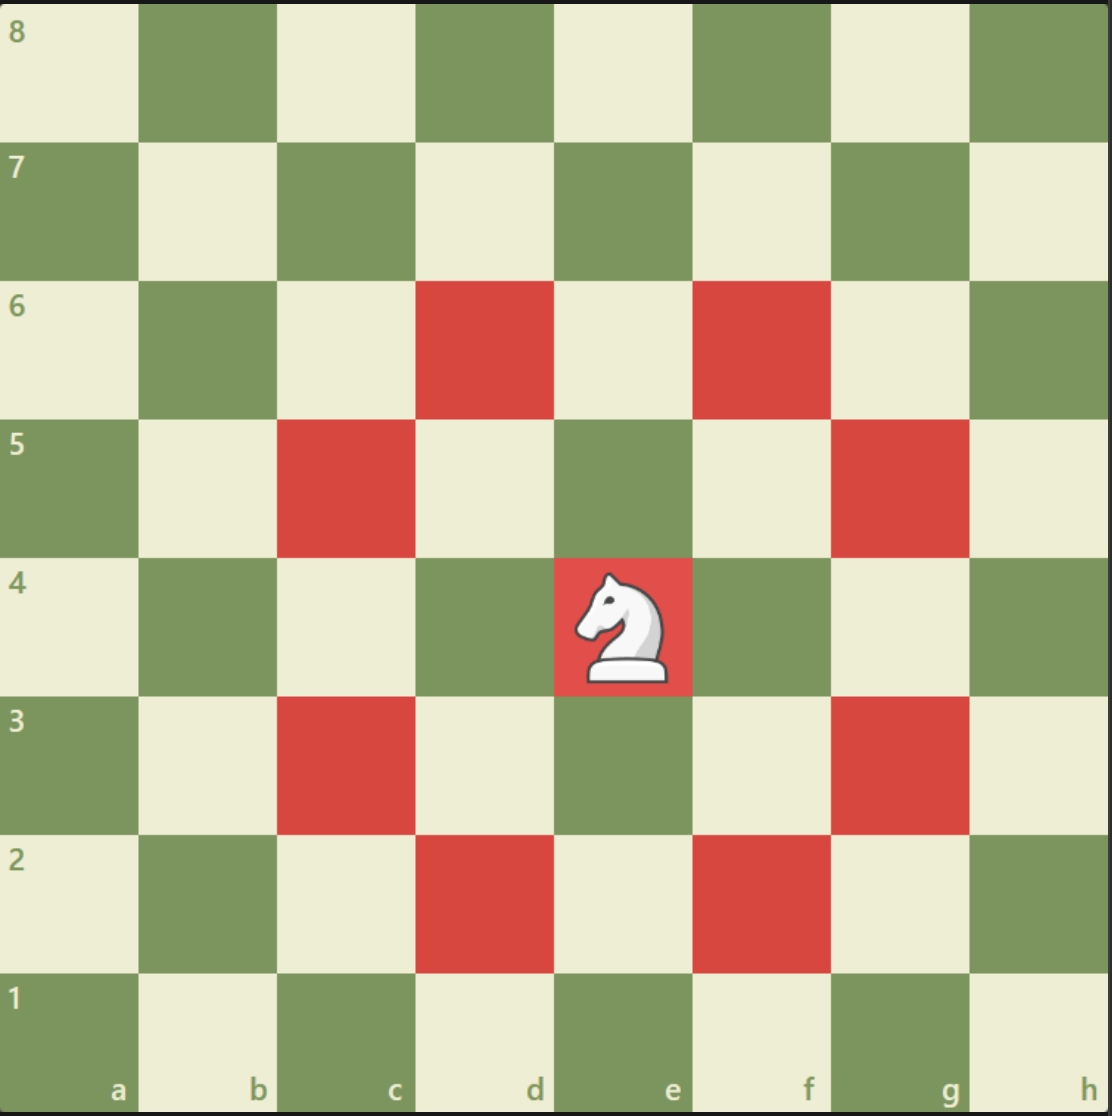
\epsfig{file=Figures/knight-moves.png, scale=0.5}} 
  \caption{The moves of a knight, courtesy of \href{https://www.chess.com/}{chess.com}.}
  \label{fig:knight-moves.png}
\end{figure}

\begin{figure}[!ht]
\centering
\begin{minted}[ frame         = lines, 
                 framesep      = 0.3cm, 
                 firstnumber   = 1,
                 bgcolor       = sepia,
                 numbers       = left,
                 numbersep     = -0.2cm,
                 xleftmargin   = 0.0cm,
                 xrightmargin  = 0.0cm,
               ]{python3}
    import z3
               
    def row(i): return f'R{i}'
    def col(i): return f'C{i}'
    
    def is_knight_move(row, col, rowX, colX):
        Formulas = set()
        for delta_r, delta_c in [(1, 2), (2, 1)]:
            Formulas.add(z3.And(rowX == row + delta_r, colX == col + delta_c))
            Formulas.add(z3.And(rowX == row + delta_r, colX + delta_c == col))
            Formulas.add(z3.And(rowX + delta_r == row, colX == col + delta_c))
            Formulas.add(z3.And(rowX + delta_r == row, colX + delta_c == col)) 
        return z3.Or(*Formulas)
            
    def all_different(Rows, Cols):
        Result = set()
        for i in range(62+1):
            for j in range (i+1, 63+1):
                Result.add(z3.Or(Rows[i] != Rows[j], Cols[i] != Cols[j]))
        return Result
            
    def all_constraints(Rows, Cols):
        Constraints = all_different(Rows, Cols)
        Constraints.add(Rows[0] == 0)
        Constraints.add(Cols[0] == 0)
        for i in range(62+1):
            Constraints.add(is_knight_move(Rows[i], Cols[i], Rows[i+1], Cols[i+1]))
        for i in range(63+1):
            Constraints.add(Rows[i] >= 0) 
            Constraints.add(Cols[i] >= 0) 
        return Constraints
\end{minted}
\vspace*{-0.3cm}
\caption{The Knight's Tour: Computing the constraints.}
\label{fig:Knight's Tour with Z3.ipynb-1}
\end{figure}



Figure \ref{fig:Knight's Tour with Z3.ipynb-1} shows how we can formulate the puzzle using \texttt{Z3}.
\begin{enumerate}
\item In line 1 we import the library \texttt{z3}.
 
\item We define the auxiliary functions \texttt{row} and \texttt{col} in line 3 and 4.
      Given a natural number $i$, the expression $\mathtt{row}(i)$ returns the string $\texttt{'R}i\texttt{'}$
      and  $\mathtt{col}(i)$ returns the string  $\texttt{'C}i\texttt{'}$.  These strings in turn represent the
      variables $\mathtt{R}_i$ and $\mathtt{C}_i$.
\item The function \texttt{is\_knight\_move} takes four parameters:
      \begin{enumerate}
      \item \texttt{row} is a \texttt{Z3} variable that specifies the row of the position of the knight before
            the move. 
      \item \texttt{col} is a \texttt{Z3} variable that specifies the column of the position of the knight
            before the move. 
      \item \texttt{rowX} is a \texttt{Z3} variable that specifies the row of the position of the knight after
            the move. 
      \item \texttt{colX} is a \texttt{Z3} variable that specifies the column of the position of the knight
            after the move. 
      \end{enumerate}
      The function checks whether the move from position 
      $\langle \mathtt{R}_i, \mathtt{C}_i \rangle$ to the position $\langle \mathtt{R}_{i+1}, \mathtt{C}_{i+1} \rangle$
      is a legal move for a knight.  In line 13 we use the fact that the function \texttt{z3.Or}
      can take any number of arguments.  If \texttt{Formulas} is the set 
      \\[0.2cm]
      \hspace*{1.3cm}
      $\texttt{Formulas} = \{f_1, \cdots, f_n\}$,
      \\[0.2cm]
      then the notation \texttt{z3.Or(*Formulas)} is expanded into the call
      \\[0.2cm]
      \hspace*{1.3cm}
      $\texttt{z3.Or}(f_1, \cdots, f_n)$,
      \\[0.2cm]
      which computes the logical disjunction
      \\[0.2cm]
      \hspace*{1.3cm}
      $f_1 \vee \cdots \vee f_n$.
\item The function \texttt{all\_different} takes two parameters:
      \begin{enumerate}[(a)]
      \item \texttt{Rows} is a list of \texttt{Z3} variables. The \texttt{Z3} variable \texttt{Rows[i]}
            specifies the row of the position of the knight after the $i^{\textrm{th}}$ move. 
      \item \texttt{Cols} is a list of \texttt{Z3} variables. The \texttt{Z3} variable \texttt{Cols[i]}
            specifies the column of the position of the knight after the $i^{\textrm{th}}$ move. 
      \end{enumerate}
      The function computes a set of formulas that state that the positions
      $\langle \mathtt{R}_i, \mathtt{C}_i \rangle$ for $i=0,1\cdots, 63$ are all different from each other.
      Note that the position $\langle \mathtt{R}_i, \mathtt{C}_i \rangle$ is different from the position
      $\langle \mathtt{R}_j, \mathtt{C}_j \rangle$ iff $R_i$ is different from $R_j$ or $C_i$ is different from
      $C_j$. 
\item The function \texttt{all\_constraints} computes the set of all constraints.
      The parameters for this function are the same as those for the function \texttt{all\_different}.
      In addition to the constraints already discussed this function specifies that the knight starts
      its tour at the upper left corner of the board.

      Furthermore, there are constraints that the variables $\mathtt{R}_i$ and $\mathtt{C}_i$ are all
      non-negative.  These constraints are needed as we will model the variables with bit vectors of length 4.
      These bit vectors store integers in
      \href{https://en.wikipedia.org/wiki/Two%27s_complement}{two's complement} representation.
      In two's complement representation of a bit vector of length 4 we can model integers from the set
      $\{-8, \cdots, 7\}$.  If we add the number $1$ to a 4-bit bit vector $v$ that represents the number $7$,
      then an overflow will occur and the result will be $-8$ instead of $8$. This could happen in the
      additions that are performed in the formulas computed by the function \texttt{is\_knight\_move}.
      We can exclude these cases by adding the constraints that all variables are non-negative.
\end{enumerate}

\begin{figure}[!ht]
\centering
\begin{minted}[ frame         = lines, 
                 framesep      = 0.3cm, 
                 firstnumber   = 1,
                 bgcolor       = sepia,
                 numbers       = left,
                 numbersep     = -0.2cm,
                 xleftmargin   = 0.8cm,
                 xrightmargin  = 0.8cm,
               ]{python3}
    def solve():
        Rows = [z3.BitVec(row(i), 4) for i in range(63+1)]
        Cols = [z3.BitVec(col(i), 4) for i in range(63+1)]
        Constraints = all_constraints(Rows, Cols)
        S = z3.Solver()
        S.add(Constraints)
        result = str(S.check())
        if result == 'sat':
            Model    = S.model()
            Solution = (  { row(i): Model[Rows[i]] for i in range(63+1) } 
                        | { col(i): Model[Cols[i]] for i in range(63+1) })
            return Solution
        elif result == 'unsat':
            print('The problem is not solvable.')
        else:
            print('Z3 cannot determine whether the problem is solvable.')
\end{minted}
\vspace*{-0.3cm}
\caption{The function \texttt{solve}.}
\label{fig:Knight's Tour with Z3.ipynb-2}
\end{figure}

\begin{figure}[!ht]
  \centering
  \framebox{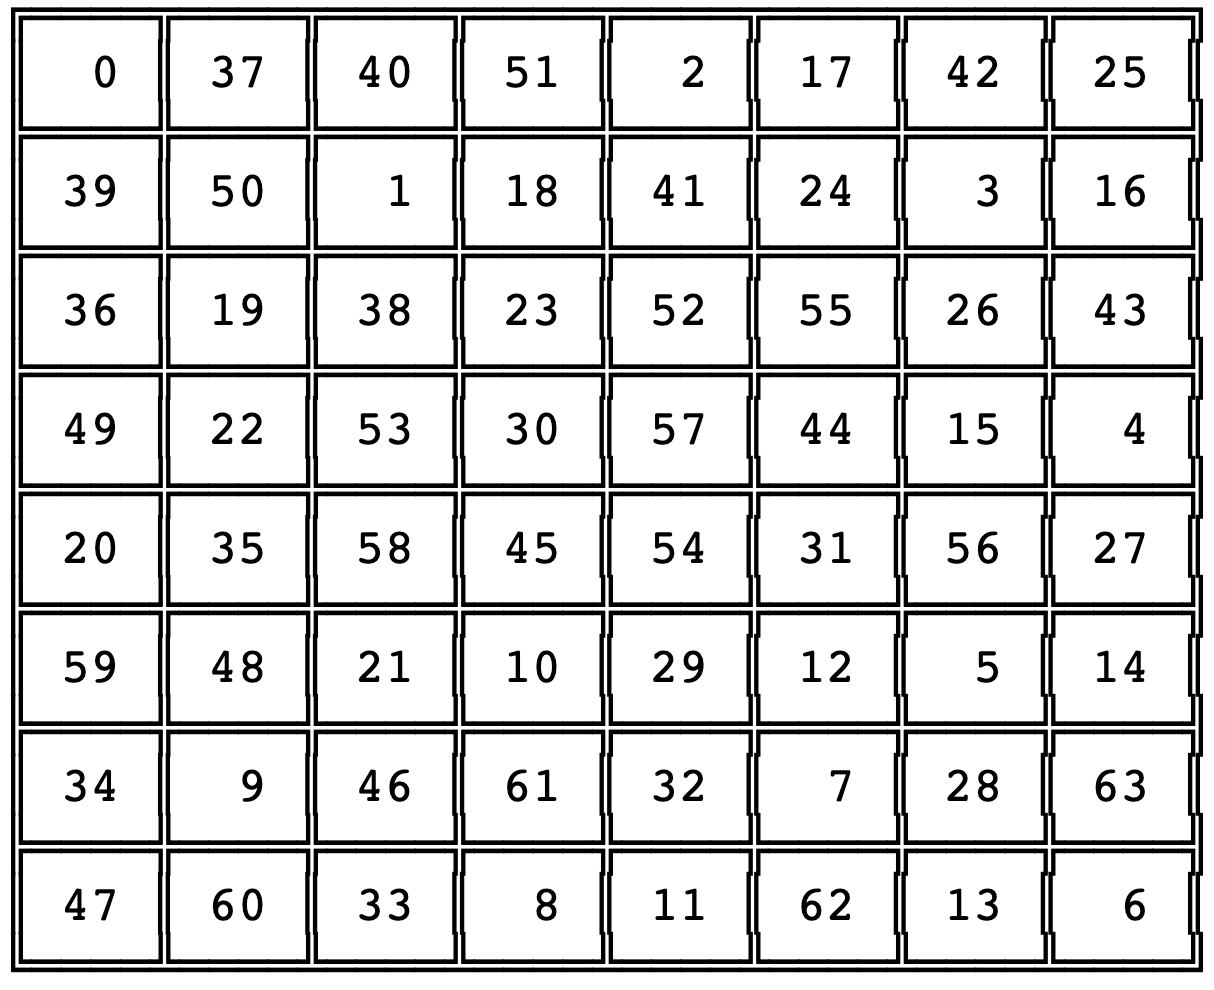
\epsfig{file=Figures/knights-problem.png, scale=0.5}} 
  \caption{A solution of the knight's problem.}
  \label{fig:knights-problem.png}
\end{figure}

Finally, the function \texttt{solve} that is shown in Figure \ref{fig:Knight's Tour with Z3.ipynb-2} on page
\pageref{fig:Knight's Tour with Z3.ipynb-2} can be used to solve the puzzle.
The purpose of the function \texttt{solve} is to construct a \textsc{Csp} encoding the puzzle and to find a
solution of this \textsc{Csp} unsing \texttt{Z3}.
If successful, it returns a dictionary that maps every variable name to the corresponding value of the solution
that has been found.
\begin{enumerate}
\item In line 2 and 3 we create the \texttt{Z3} variables that specify the positions of the knight after its
      $i^{\mathrm{th}}$ move.  $\texttt{Rows}[i]$ specifies the row of the knight after the its
      $i^{\mathrm{th}}$ move, while $\texttt{Cols}[i]$ specifies the column.
\item We compute the set of all constraints in line 4.   
\item We create a solver object in line 5 and add the constraints to this solver in the following line.
\item The function \texttt{check} tries to build a model satisfying the constraints, while the function
      \texttt{model} extracts this model if it exists.
\item Finally, in line 10 and 11 we create a dictionary that maps all of our variables to the corresponding
      values that are found in the model.  Note that $\texttt{row}(i)$ returns the name of the
      \texttt{Z3} variable $\texttt{Rows}[i]$ and similarly $\mathtt{col}(i)$ returns the name of the
      \texttt{Z3} variable $\texttt{Cols}[i]$.
      This dictionary is then returned.
\end{enumerate}
Figure \ref{fig:knights-problem.png} on page \pageref{fig:knights-problem.png} shows a solution that has been
computed by the program discussed above.


\begin{table}[h]
  \centering
  \begin{tabular}{||c|c|c||c|c|c||c|c|c||}
    \hline
    \hline
      & 3 & 9 &   &   &   &   &   & 7 \\
    \hline
      &   &   & 7 &   &   & 4 & 9 & 2 \\
    \hline
      &   &   &   & 6 & 5 &   & 8 & 3 \\
    \hline
    \hline
      &   &   & 6 &   & 3 & 2 & 7 &   \\
    \hline
      &   &   &   & 4 &   & 8 &   &   \\
    \hline
    5 & 6 &   &   &   &   &   &   &   \\
    \hline
    \hline
      &   & 5 & 2 &   & 9 &   &   & 1 \\
    \hline
      & 2 & 1 &   &   &   &   & 4 &   \\
    \hline
    7 &   &   &   &   &   & 5 &   &   \\
    \hline
    \hline
  \end{tabular}
  \caption{A super hard sudoku from the magazine ``Zeit Online''.}
  \label{tab:sudoku}
\end{table}


\exerciseEng
\index{sudoku}
Table \ref{tab:sudoku} on page \pageref{tab:sudoku} shows a \href{https://en.wikipedia.org/wiki/Sudoku}{sudoku}
that I have taken from the
\href{http://sudoku.zeit.de/cgi-bin/sudoku/sudoku_kd_app_2016.pl?action=level&kd_nr=24091123601092&year=2018&month=03&day=23&level=-c+5}{Zeit Online}
magazine.
Solve this sudoku using \texttt{Z3}.  You should start with the following file:
\\[0.2cm]
\hspace*{0.0cm}
\href{https://github.com/karlstroetmann/Logic/blob/master/Python/Chapter-5/Sudoku-Z3.ipynb}{https://github.com/karlstroetmann/Logic/blob/master/Python/Chapter-5/Sudoku-Z3.ipynb}.
    \eox

\section{Normalformen für prädikatenlogische Formeln}
Im nächsten Abschnitt gehen wir daran, einen Kalkül $\vdash$ für die
Prädikaten-Logik zu definieren.  Genau wie im Falle der Aussagen-Logik wird dies wesentlich einfacher, wenn wir
uns auf Formeln beschränken, die in einer \blue{Normalform}  vorliegen.  Bei dieser Normalform handelt es sich
nun um sogenannte \blue{prädikatenlogische Klauseln}.\index{prädikatenlogische Klausel}  Diese werden ähnlich
definiert wie in der 
Aussagen-Logik:  Ein \blue{prädikatenlogisches Literal}\index{prädikatenlogisches Literal} ist eine atomare
Formel oder die Negation einer 
atomaren Formel.  Eine \blue{prädikatenlogische Klausel}\index{prädikatenlogische Klausel} ist dann eine
Disjunktion prädikatenlogischer Literale.  Wir zeigen in diesem Abschnitt, dass jede Formel-Menge $M$
so in eine Menge von prädikatenlogischen Klauseln $K$ transformiert werden kann, dass $M$ genau dann erfüllbar ist, wenn $K$
erfüllbar ist.  Daher ist die Beschränkung auf prädikatenlogische Klauseln keine echte Einschränkung.  Zunächst geben wir einige
Äquivalenzen an, mit deren Hilfe Quantoren manipuliert werden können. 

\begin{Satz}
  Es gelten die folgenden Äquivalenzen:
  \begin{enumerate}
  \item $\models \neg\big(\forall x\colon f\big) \leftrightarrow \big(\exists x\colon \neg f\big)$
  \item $\models \neg\big(\exists x\colon f\big) \leftrightarrow \big(\forall x\colon \neg f\big)$
  \item $\models \forall x\colon f \wedge \forall x\colon g \leftrightarrow \forall x\colon (f \wedge g)$
  \item $\models \exists x\colon f \vee \exists x\colon g \leftrightarrow \exists x\colon (f \vee g)$
  \item $\models \forall x\colon \forall y\colon f \leftrightarrow \forall y\colon  \forall x\colon f$
  \item $\models \exists x\colon \exists y\colon f \leftrightarrow \exists y\colon  \exists x\colon f$
  \item Falls $x$ eine Variable ist, für die $x \not\in \FV(f)$ ist, so haben wir \\[0.2cm]
        \hspace*{1.3cm} $\models  (\forall x\colon f) \leftrightarrow f$ \quad und \quad
                        $\models  (\exists x\colon f) \leftrightarrow f$.
  \item Falls $x$ eine Variable ist, für die  $x \not\in \FV(g)$ gilt, so haben wir die folgenden Äquivalenzen:
    \begin{enumerate}
    \item $\models (\forall x\colon f) \vee g \leftrightarrow \forall x\colon (f \vee g)$ \quad und \quad $\models g \vee (\forall x\colon f) \leftrightarrow \forall x\colon (g \vee f)$,
    \item $\models (\exists x\colon f) \wedge g \leftrightarrow \exists x\colon (f \wedge g)$ \quad und \quad $\models g \wedge (\exists x\colon f) \leftrightarrow \exists x\colon (g \wedge f)$.
    \end{enumerate}
  \end{enumerate}
\end{Satz}

Um die Äquivalenzen der letzten Gruppe anwenden zu können, kann es notwendig sein,
gebundene Variablen umzubenennen. Ist $f$ eine prädikatenlogische Formel und sind $x$ und
$y$ zwei Variablen, wobei $y$ nicht in $f$ auftritt, so bezeichnet \blue{$f[x/y]$} die Formel, die aus $f$
dadurch entsteht, dass jedes Auftreten der Variablen $x$ in $f$ durch $y$ ersetzt wird.  Beispielsweise gilt \\[0.2cm]
\hspace*{1.3cm} $\bigl(\forall u : \exists v : p(u,v)\bigr)[u/z] = \forall z : \exists v : p(z,v)$
\\[0.2cm]
Damit können wir eine letzte Äquivalenz angeben: Ist $f$ eine prädikatenlogische Formel,
ist $x \in BV(f)$ und ist $y$ eine Variable, die in $f$ nicht auftritt, so gilt \\[0.2cm]
\hspace*{1.3cm} $\models f \leftrightarrow f[x/y]$.
\vspace{0.3cm}

Mit Hilfe der oben stehenden Äquivalenzen und der aussagenlogischen Äquivalenzen, die wir schon kennen, können
wir eine Formel so umformen, dass die Quantoren nur noch außen stehen.  Eine solche Formel ist dann in
\blue{pränexer Normalform}.\index{pränexer Normalform}  Wir führen das Verfahren an einem Beispiel vor: Wir
zeigen, dass die Formel  
\\[0.2cm]
\hspace*{1.3cm}
$\bigl(\forall x\colon p(x)\bigr) \rightarrow \bigl(\exists x\colon p(x)\bigr)$ 
\\[0.2cm]
allgemeingültig ist: 
$$ 
\begin{array}{ll}
                 & \bigl(\forall x\colon p(x)\bigr) \rightarrow \bigl(\exists x\colon p(x)\bigr)  \\
 \Leftrightarrow & \neg \bigl(\forall x\colon p(x)\bigr) \vee \bigl(\exists x\colon p(x)\bigr)    \\
 \Leftrightarrow & \bigl(\exists x\colon \neg p(x)\bigr) \vee \bigl(\exists x\colon p(x)\bigr)    \\
 \Leftrightarrow & \exists x\colon \bigl(\neg p(x) \vee p(x)\bigr) \\
 \Leftrightarrow & \exists x\colon \verum                                                  \\
 \Leftrightarrow & \verum                                                  \\
\end{array}
$$
\\[0.2cm]
In diesem Fall haben wir Glück gehabt, dass es uns gelungen ist, die Formel als Tautologie zu
erkennen.  Im Allgemeinen reichen die obigen Umformungen aber nicht aus, um prädikatenlogische
Tautologien erkennen zu können.  Um Formeln noch stärker vereinfachen zu können, 
führen wir einen weiteren Äquivalenz-Begriff ein.  Diesen Begriff wollen wir vorher durch ein Beispiel
motivieren.  Wir betrachten die beiden Formeln 
\\[0.2cm]
\hspace*{1.3cm} $f_1 = \forall x \colon \exists y \colon p(x,y)$ \quad und \quad $f_2 = \forall x \colon
p\bigl(x,s(x)\bigr)$.
\\[0.2cm]
Die beiden Formeln $f_1$ und $f_2$ sind nicht äquivalent, denn sie entstammen noch nicht
einmal der gleichen Signatur: In der Formel $f_2$ wird das Funktions-Zeichen $s$
verwendet, das in der Formel $f_1$ überhaupt nicht auftritt. 
Auch wenn die beiden Formeln $f_1$ und $f_2$ nicht äquivalent sind, so besteht zwischen
ihnen doch die folgende Beziehung:  Ist $\textsl{S}_1$ eine
prädikatenlogische Struktur, in der die Formel $f_1$ gilt:
\\[0.2cm]
\hspace*{1.3cm}
$\mathcal{S}_1 \models f_1$,
\\[0.2cm]
dann können wir diese Struktur zu einer Struktur $\textsl{S}_2$ erweitern, in der die
Formel $f_2$ gilt:
\\[0.2cm]
\hspace*{1.3cm}
$\mathcal{S}_2 \models f_2$.
\\[0.2cm]
Dazu muss die Interpretation des Funktions-Zeichens $s$ so gewählt werden, dass
für jedes $x$ tatsächlich $p\bigl(x,s(x)\bigr)$ gilt.  Dies ist möglich, denn die Formel $f_1$ sagt ja aus, 
dass wir zu jedem $x$ einen Wert $y$ finden, für den $p(x,y)$ gilt.   Die Funktion $s$ muss also lediglich zu 
jedem $x$ dieses $y$ zurück geben. 



\begin{Definition}[{\color{blue}Skolemisierung}]\index{Skolemisierung} \hspace*{\fill} \linebreak
  Es sei $\Sigma = \langle \mathcal{V}, \mathcal{F}, \mathcal{P}, \textsl{arity} \rangle$
  eine Signatur.  Ferner sei $f$ eine geschlossene $\Sigma$-Formel der Form \\[0.2cm]
  \hspace*{1.3cm} 
  $f = \forall x_1, \cdots, x_n \colon \exists y \colon g$. \\[0.2cm]
  Dann wählen wir ein \underline{\blue{neues}} $n$-stelliges Funktions-Zeichen $s$, d.h.~wir nehmen ein Zeichen $s$, dass in
  der Signatur $\Sigma$ nicht auftritt und erweitern die Signatur $\Sigma$ zu der Signatur \\[0.2cm]
  \hspace*{1.3cm} 
  $\Sigma' := \Bigl\langle \mathcal{V}, \mathcal{F} \cup \{s\}, \mathcal{P}, \textsl{arity} \cup \bigl\{\pair(s,n)\bigr\} \Bigr\rangle$, \\[0.2cm]
  in der wir $s$ als neues $n$-stelliges Funktions-Zeichen deklarieren.  Anschließend definieren wir die $\Sigma'$-Formel
  $f'$ wie folgt: \\[0.2cm]
  \hspace*{1.3cm} 
  $f' := \mathtt{Skolem}(f) := 
  \forall x_1 \colon \cdots \forall x_n \colon g\bigl[y \mapsto s(x_1,\cdots,x_n)\bigr]$
  \\[0.2cm]
  Hierbei bezeichnet der Ausdruck $g\bigl[y \mapsto s(x_1,\cdots,x_n)\bigr]$ die Formel, die wir aus $g$
  dadurch erhalten, dass wir jedes Auftreten der Variablen $y$ in der Formel $g$ durch den Term
  $s(x_1,\cdots,x_n)$ ersetzen.  Wir sagen, dass die Formel $f'$ aus der Formel $f$
  durch einen \blue{Skolemisierungs-Schritt} hervorgegangen ist. 
  \eox
\end{Definition}
\vspace{-0.5cm}

\example
Es $f$ die folgende Formel aus der Gruppen-Theorie:
\\[0.2cm]
\hspace*{1.3cm}
$f := \forall x: \exists y: y * x = 1$. 
\\[0.2cm]
Dann gilt
\\[0.2cm]
\hspace*{1.3cm}
$\mathtt{Skolem}(f) = \forall x : s(x) * x = 1$.  \eox

\noindent
In welchem Sinne sind eine Formel $f$ und eine Formel $f'$, die aus $f$ durch einen 
Skolem\-isierungs-Schritt hervorgegangen sind, äquivalent?  Zur Beantwortung dieser Frage
dient die folgende Definition. 

\begin{Definition}[Erfüllbarkeits-Äquivalenz] \hspace*{\fill} \linebreak
   Zwei geschlossene Formeln $f$ und $g$ heißen 
   \blue{erfüllbarkeits-äquivalent}\index{erfüllbarkeits-äquivalent}
   falls $f$ und $g$ entweder beide erfüllbar oder beide unerfüllbar sind.
   Wenn $f$ und $g$ erfüllbarkeits-äquivalent sind, so schreiben wir \\[0.2cm]
   \hspace*{1.3cm} $f \approx_e g$.
\eox
\end{Definition}

\noindent
\textbf{Beobachtung:}
Falls die Formel $f'$ aus der Formel $f$ durch einen Skolemisierungs-Schritt 
hervorgegangen ist, so sind $f$ und $f'$ erfüllbarkeits-äquivalent, denn wir können jede Struktur
$\mathcal{S}$, in der die Formel $f$ gilt, zu einer Struktur $\mathcal{S}'$ erweitern, in der auch $f'$ gilt.
\eox

Wir können nun ein einfaches Verfahren angeben, um Existenz-Quantoren aus einer Formel
zu eliminieren.  Dieses Verfahren besteht aus zwei Schritten:  Zunächst bringen wir die Formel
in pränexe Normalform. Anschließend können wir die Existenz-Quantoren der Reihe nach durch \linebreak
Skolemisierungs-Schritte eliminieren.  Nach dem oben gemachten Bemerkungen ist die resultierende 
Formel zu der ursprünglichen Formel erfüllbarkeits-äquivalent.  Dieses
Verfahren der Eliminierung von Existenz-Quantoren durch die Einführung neuer
Funktions-Zeichen wird als \blue{Skolemisierung} bezeichnet.  Haben wir eine Formel $F$
in pränexe Normalform gebracht und anschließend skolemisiert, so hat das Ergebnis die Gestalt\\[0.2cm]
\hspace*{1.3cm} $\forall x_1, \cdots, x_n: g$ \\[0.2cm]
und in der Formel $g$ treten keine Quantoren mehr auf.  Die Formel $g$ wird auch als die
\blue{Matrix}\index{Matrix} der obigen Formel bezeichnet.  Wir können nun  $g$ mit Hilfe
der uns aus dem letzten Kapitel bekannten aussagenlogischen
 Äquivalenzen in konjunktive Normalform bringen.  Wir haben dann eine
Formel der Gestalt \\[0.2cm]
\hspace*{1.3cm} $\forall x_1, \cdots, x_n: (k_1 \wedge \cdots \wedge k_m)$. \\[0.2cm]
Dabei sind die $k_i$ Disjunktionen von prädikatenlogischen \blue{Literalen}.  Wenden wir
hier  die Äquivalenz 
\\[0.2cm]
\hspace*{1.3cm}
$\forall x\colon (f_1\wedge f_2) \leftrightarrow (\forall x\colon f_1) \wedge (\forall x\colon f_2)$
\\[0.2cm]
an, so können wir die All-Quantoren auf die einzelnen $k_i$ verteilen und
die resultierende Formel hat die Gestalt \\[0.2cm]
\hspace*{1.3cm} 
$\big(\forall x_1, \cdots, x_n: k_1\big) \wedge \cdots \wedge \big(\forall x_1, \cdots, x_n: k_m\big)$. \\[0.2cm]
Ist eine Formel $F$ in der obigen
Gestalt, so sagen wir, dass $F$ in \blue{prädikatenlogischer Klausel-Normalform}
\index{prädikatenlogische Klausel-Normalform}  ist und eine Formel der Gestalt \\[0.2cm]
\hspace*{1.3cm} $\forall x_1, \cdots, x_n: k$, \\[0.2cm]
bei der $k$ eine Disjunktion prädikatenlogischer Literale ist,
bezeichnen wir als \blue{prädikatenlogische Klausel}.  \index{prädikatenlogische Klausel} Ist $M$
eine Menge von Formeln deren Erfüllbarkeit wir untersuchen wollen, so können wir nach dem
bisher Gezeigten  $M$ immer in eine erfüllbarkeits-äquivalente Menge prädikatenlogischer Klauseln umformen.
Da  dann nur noch All-Quantoren vorkommen, können wir hier die  Notation noch vereinfachen,
indem wir vereinbaren, dass alle Formeln implizit allquantifiziert sind, wir lassen also
die All-Quantoren weg.

\noindent
Das Jupyter Notebook
\\[0.2cm]
\hspace*{0.8cm}
\href{https://github.com/karlstroetmann/Logic/blob/master/Python/Chapter-5/FOL-CNF.ipynb}{https://github.com/karlstroetmann/Logic/blob/master/Python/Chapter-5/FOL-CNF.ipynb}.
\\[0.2cm]
enthält ein \textsl{Python}-Programm, mit dessen Hilfe wir prädikatenlogische Formeln in eine \linebreak
erfüllbarkeits-äquivalente Menge von prädikatenlogischen Klauseln umformen können.

Wozu sind nun die Umformungen in Skolem-Normalform gut?  Es geht darum, dass wir 
ein Verfahren entwickeln wollen, mit dem es möglich ist für eine prädikatenlogische Formel
$f$ zu zeigen, dass $f$ allgemeingültig ist, dass also \\[0.2cm]
\hspace*{1.3cm} $\models f$ \\[0.2cm]
gilt.  Wir wissen, dass \\[0.2cm]
\hspace*{1.3cm} $\models f$ \quad g.d.w. \quad $\{\neg f\} \models \falsum$ \\[0.2cm]
gilt, denn die Formel $f$ ist genau dann allgemeingültig, wenn es keine Struktur gibt, in
der die Formel $\neg f$ erfüllbar ist. 
 Wir bilden daher zunächst die Formel $\neg f$ und formen dann diese Formel in prädikatenlogische
Klausel-Normalform um.  Wir erhalten Klauseln $k_1, \cdots, k_n$, so dass  \\[0.2cm]
\hspace*{1.3cm} $\neg f \approx_e k_1 \wedge \cdots \wedge k_n$ \\[0.2cm]
gilt.  Anschließend versuchen wir,
aus den Klauseln $k_1,\cdots,k_n$ einen Widerspruch herzuleiten: \\[0.2cm]
\hspace*{1.3cm} $\{k_1, \cdots, k_n\} \vdash \falsum$ \\[0.2cm]
Wenn dies gelingt, dann wissen wir, dass die Menge $\{k_1, \cdots, k_n\}$ unerfüllbar ist.
Damit ist auch $\neg f$ unerfüllbar und also ist $f$ allgemeingültig.
Damit wir aus den Klauseln $k_1,\cdots,k_n$ einen Widerspruch herleiten können,
brauchen wir natürlich noch einen Kalkül $\vdash$, der mit prädikatenlogischen Klauseln arbeitet. 
Einen solchen Kalkül werden wir im übernächsten Abschnitt vorstellen.

Um das Verfahren näher zu erläutern demonstrieren wir es an einem Beispiel. 
Wir wollen untersuchen, ob \\[0.2cm]
\hspace*{1.3cm} 
$\models \big(\exists x\colon \forall y\colon  p(x,y)\big) \rightarrow \big(\forall y\colon \exists x\colon p(x,y)\big)$ \\[0.2cm]
gilt.  Wir wissen, dass dies äquivalent dazu ist, dass  \\[0.2cm]
\hspace*{1.3cm} 
$\Big\{ \neg \Big(\big(\exists x\colon \forall y\colon  p(x,y)\big) \rightarrow  \big(\forall y\colon \exists x\colon p(x,y)\big)\Big)\Big\} \models \falsum$ \\[0.2cm]
gilt.  Wir bringen zunächst die negierte Formel in pränexe Normalform. 
$$
\begin{array}{ll}
                  & \neg \Big(\big(\exists x\colon \forall y\colon  p(x,y)\big) \rightarrow \big(\forall y\colon \exists x\colon p(x,y)\big)\Big) \\
  \leftrightarrow & \neg \Big(\neg \big(\exists x\colon \forall y\colon  p(x,y)\big) \vee \big(\forall y\colon \exists x\colon p(x,y)\big)\Big) \\
  \leftrightarrow &                \big(\exists x\colon \forall y\colon  p(x,y)\big) \wedge \neg \big(\forall y\colon \exists x\colon p(x,y)\big) \\
  \leftrightarrow &\big(\exists x\colon \forall y\colon  p(x,y)\big) \wedge  \big(\exists y\colon  \neg \exists x\colon p(x,y)\big) \\
  \leftrightarrow &\big(\exists x\colon \forall y\colon  p(x,y)\big) \wedge  \big(\exists y\colon  \forall x\colon \neg p(x,y)\big) \\
\end{array}
$$
Um an dieser Stelle weitermachen zu können, ist es nötig, die Variablen in dem  zweiten
Glied der Konjunktion umzubenennen.  Wir ersetzen $x$ durch $u$ und $y$ durch $v$ und erhalten
$$
\begin{array}{ll}
                  &\big(\exists x\colon \forall y\colon  p(x,y)\big) \wedge  \big(\exists y\colon  \forall x\colon \neg p(x,y)\big) \\
  \leftrightarrow &\big(\exists x\colon \forall y\colon  p(x,y)\big) \wedge  \big(\exists v\colon  \forall u\colon \neg p(u,v)\big) \\
  \leftrightarrow &\exists v\colon  \Big( \big(\exists x\colon \forall y\colon  p(x,y)\big) \wedge  \big(\forall u\colon \neg p(u,v)\big) \Big)\\
  \leftrightarrow &\exists v\colon  \exists x\colon  \Big( \big(\forall y\colon  p(x,y)\big) \wedge \big(\forall u\colon \neg p(u,v)\big) \Big)\\
  \leftrightarrow &\exists v\colon  \exists x\colon \forall y\colon \Big( p(x,y) \wedge \big(\forall u\colon \neg p(u,v)\big) \Big)\\
  \leftrightarrow &\exists v\colon  \exists x\colon \forall y\colon \forall u\colon \Big( p(x,y) \wedge \neg p(u,v) \Big)\\
\end{array}
$$
An dieser Stelle müssen wir skolemisieren um die Existenz-Quantoren los zu werden. 
Wir führen dazu zwei neue Funktions-Zeichen $s_1$ und $s_2$ ein. 
Dabei gilt $\mathtt{arity}(s_1) = 0$ und $\mathtt{arity}(s_2) = 0$, denn vor den
Existenz-Quantoren stehen keine All-Quantoren.
$$
\begin{array}{ll}
           & \exists v\colon  \exists x\colon \forall y\colon \forall u\colon \Big( p(x,y) \wedge \neg p(u,v) \Big)\\
 \approx_e & \exists x\colon \forall y\colon \forall u\colon \Big( p(x,y) \wedge \neg p(u,s_1) \Big)\\
 \approx_e & \forall y\colon \forall u\colon \Big( p(s_2,y) \wedge \neg p(u,s_1) \Big)\\
\end{array}
$$
Da jetzt nur noch All-Quantoren auftreten, können wir diese auch noch weglassen,
da wir ja ver\-einbart haben, dass alle freien Variablen implizit allquantifiziert sind.
Damit können wir nun die prädikatenlogische Klausel-Normalform in Mengen-Schreibweise angeben, diese
ist
\\[0.2cm] 
\hspace*{1.3cm}
$M := \Big\{ \big\{ p(s_2,y) \big\}, \big\{\neg p(u,s_1)\big\}\Big\}$.
\\[0.2cm]
Wir zeigen, dass die Menge $M$ widersprüchlich ist.
Dazu betrachten wir zunächst die Klausel $\big\{ p(s_2,y) \big\}$ und setzen in
dieser Klausel für $y$ die Konstante $s_1$ ein.  Damit erhalten wir die Klausel \\[0.2cm]
\hspace*{1.3cm}  $\big\{ p(s_2,s_1) \big\}$. \hspace*{\fill}(1)\\[0.2cm]
Das Ersetzung von $y$ durch $s_1$ begründen wir damit, dass die obige Klausel ja implizit
allquantifiziert ist und wenn etwas für alle $y$ gilt, dann sicher auch für $y = s_1$.

Als nächstes betrachten wir die Klausel $\big\{\neg p(u,s_1)\big\}$.
Hier setzen wir für die Variablen $u$ die Konstante $s_2$ ein und erhalten dann die
Klausel \\[0.2cm]
\hspace*{1.3cm} $\big\{\neg p(s_2,s_1)\big\}$ \hspace*{\fill} (2) \\[0.2cm]
Nun wenden wir auf die Klauseln (1) und (2) die Schnitt-Regel an und finden \\[0.2cm]
\hspace*{1.3cm} 
$\big\{ p(s_2,s_1) \big\}$, \quad$\big\{\neg p(s_2,s_1)\big\}$ \quad $\vdash \quad \{\}$.
\\[0.2cm]
Damit haben wir einen Widerspruch hergeleitet und gezeigt, dass die Menge $M$ unerfüllbar
ist. Damit ist dann auch \\[0.2cm]
\hspace*{1.3cm} 
$\Big\{ \neg \Big(\big(\exists x\colon \forall y\colon  p(x,y)\big) \rightarrow  \big(\forall y\colon \exists x\colon p(x,y)\big)\Big)\Big\}$
\\[0.2cm]
unerfüllbar und folglich gilt \\[0.2cm]
\hspace*{1.3cm} 
$\models \big(\exists x\colon \forall y\colon  p(x,y)\big) \rightarrow  \big(\forall y\colon \exists x\colon p(x,y)\big)$.

\section{Unifikation}
In dem  Beispiel im letzten Abschnitt haben wir die Terme $s_1$ und $s_2$ geraten, die wir für die Variablen
$y$ und $u$ in den Klauseln $\big\{ p(s_2,y) \big\}$ und  $\big\{\neg p(u,s_1)\big\}$
eingesetzt haben.  Wir haben diese Terme mit dem Ziel gewählt, später die Schnitt-Regel
anwenden zu können.  In diesem Abschnitt zeigen wir nun ein Verfahren, mit dessen Hilfe
wir die benötigten Terme ausrechnen können.
Dazu benötigen wir zunächst den Begriff einer \blue{Substitution}.
\begin{Definition}[Substitution]\index{Substitution}
    Es sei eine Signatur \\[0.2cm]
    \hspace*{1.3cm} $\Sigma = \langle \mathcal{V}, \mathcal{F}, \mathcal{P}, \textsl{arity} \rangle$ \\[0.2cm]
    gegeben.  Eine {\color{blue}$\Sigma$-Substitution} ist eine endliche Menge von Paaren der Form \\[0.2cm]
    \hspace*{1.3cm} $\sigma = \bigl\{ \langle x_1, t_1 \rangle, \cdots, \langle x_n, t_n \rangle \bigr\}$. \\[0.2cm]
    Dabei gilt:
    \begin{enumerate}
    \item $x_i \in \mathcal{V}$, die $x_i$ sind also Variablen.
    \item $t_i \in \mathcal{T}_\Sigma$, die $t_i$ sind also Terme.
    \item Für $i\not=j$ ist $x_i \not= x_j$, die Variablen sind also paarweise verschieden.
    \end{enumerate}
    
    Ist $\sigma = \bigl\{ \langle x_1, t_1 \rangle, \cdots, \langle x_n, t_n \rangle \bigr\}$ eine
    $\Sigma$-Substitution, so schreiben wir  \\[0.2cm]
    \hspace*{1.3cm} $\sigma = \bigl[ x_1 \mapsto t_1, \cdots, x_n \mapsto t_n \bigr]$.  \\[0.2cm]
    Außerdem definieren wir den \blue{Domain} einer Substitution als \\[0.2cm]
    \hspace*{1.3cm} $\textsl{dom}(\sigma) := \{ x_1, \cdots, x_n\}$.
    \\[0.2cm]
    Die Menge aller Substitutionen bezeichnen wir mit \blue{\textsl{Subst}}.\index{Subst}
    \eox
\end{Definition}

\noindent
Substitutionen werden für uns dadurch interessant, dass wir sie auf Terme \blue{anwenden} können.  Ist $t$ ein
Term und $\sigma$ eine Substitution, so ist $t\sigma$ der Term, der aus $t$ dadurch entsteht, dass jedes
Vorkommen einer Variablen $x_i$ durch den zugehörigen Term $t_i$ ersetzt wird.  Die formale Definition folgt. 
\begin{Definition}[Anwendung einer Substitution]
\hspace*{\fill} \\
Es sei $t$ ein Term und es sei $\sigma = \bigl[ x_1 \mapsto t_1, \cdots, x_n \mapsto t_n \bigr]$
eine Substitution. Wir definieren die \blue{Anwendung}\index{Anwending einer Substitution} von $\sigma$ auf $t$
(Schreibweise \blue{$t\sigma$}) \index{$t\sigma$} durch Induktion über 
den Aufbau von $t$: 
\begin{enumerate}
\item Falls $t$ eine Variable ist, gibt es zwei Fälle:
  \begin{enumerate}
  \item $t = x_i$ für ein $i\in\{1,\cdots,n\}$.  Dann definieren wir \quad  $x_i\sigma := t_i$.
  \item $t = y$ mit $y\in\mathcal{V}$, aber $y \not\in \{x_1,\cdots,x_n\}$. Dann definieren wir \quad $y\sigma := y$.
  \end{enumerate}
\item Andernfalls muss $t$ die Form $t= f(s_1,\cdots,s_m)$ haben. Dann können wir $t\sigma$ durch \\[0.2cm]
      \hspace*{1.3cm} $f(s_1, \cdots, s_m)\sigma := f(s_1\sigma, \cdots, s_m\sigma)$. \\[0.2cm]
      definieren, denn nach Induktions-Voraussetzung sind die Ausdrücke $s_i\sigma$ bereits definiert.      
      \eox
\end{enumerate}
\end{Definition}

Genau wie wir Substitutionen auf Terme anwenden können, können wir eine Substitution
auch auf prädikatenlogische Klauseln anwenden.  Dabei werden Prädikats-Zeichen und
Junktoren wie Funktions-Zeichen behandelt.
Wir ersparen uns eine formale Definition und geben stattdessen zunächst einige Beispiele. 
Wir definieren eine Substitution $\sigma$ durch \\[0.2cm]
\hspace*{1.3cm} $\sigma := \big[ x_1 \mapsto c,\; x_2 \mapsto f(d) \big]$. \\[0.2cm]
In den folgenden drei Beispielen demonstrieren wir zunächst, wie eine Substitution
auf einen Term angewendet werden kann.  Im vierten Beispiel wenden wir die Substitution
dann auf eine Klausel in Mengen-Schreibweise an:
\begin{enumerate}
\item $x_3\sigma = x_3$,
\item $f(x_2)\sigma = f\bigl(f(d)\bigr)$,
\item $h(x_1,g(x_2))\sigma = h\bigl(c,g(f(d))\bigr)$.
\item $\bigl\{ p(x_2), q(d,h(x_3,x_1))\bigr\}\sigma = \bigl\{ p(f(d)),\; q(d,h(x_3,c))\bigr\}$.
\end{enumerate}


\noindent
Als nächstes zeigen wir, wie  Substitutionen miteinander verknüpft werden können.
\begin{Definition}[Komposition von Substitutionen] \index{Komposition von Substitutionen}
    Es seien\\[0.2cm]
    \hspace*{1.3cm}  $\sigma = \big[ x_1 \mapsto s_1, \cdots, x_m \mapsto s_m \big]$ \quad und \quad  $\tau = \big[ y_1 \mapsto t_1, \cdots, y_n \mapsto t_n \big]$ \\[0.2cm]
    zwei Substitutionen mit $\textsl{dom}(\sigma) \cap \textsl{dom}(\tau) = \{\}$. Dann definieren
    wir die \blue{Komposition von Substitutionen} $\sigma\tau$ \index{$\sigma\tau$} von $\sigma$ und $\tau$ als \\[0.2cm]
    \hspace*{1.3cm} $\sigma\tau := \big[ x_1 \mapsto s_1\tau, \cdots, x_m \mapsto s_m\tau,\; y_1 \mapsto t_1, \cdots, y_n \mapsto t_n \big]$
    \eox
\end{Definition}

\example
Wir führen das obige Beispiel fort und setzen \\[0.2cm]
\hspace*{1.3cm} $\sigma := \big[ x_1 \mapsto c,\; x_2 \mapsto f(x_3) \big]$
                \quad und \quad $\tau := \big[ x_3 \mapsto h(c,c),\; x_4 \mapsto d \big]$. \\[0.2cm]
Dann gilt: \\[0.2cm]
\hspace*{1.3cm} $ \sigma\tau = \big[ x_1 \mapsto c,\; x_2 \mapsto f(h(c,c)),\; x_3 \mapsto h(c,c),\;x_4 \mapsto d \big]$.
\hspace*{\fill} $\Box$
\vspace{0.3cm}

\noindent
Die Definition der Komposition von Substitutionen ist mit dem Ziel gewählt worden, dass
der folgende Satz gilt.
\begin{Satz} \label{satz:komposition}
    Ist $t$ ein Term und sind $\sigma$ und $\tau$ Substitutionen mit 
    $\textsl{dom}(\sigma) \cap \textsl{dom}(\tau) = \{\}$, so gilt \\[0.2cm]
    \hspace*{1.3cm} $(t \sigma)\tau = t (\sigma\tau)$.
    \hspace*{\fill} $\Box$
\end{Satz}
Der Satz kann durch Induktion über den Aufbau des Termes $t$ bewiesen werden.


\begin{Definition}[Syntaktische Gleichung] \index{syntaktische Gleichung}
Unter einer \blue{syntaktischen Gleichung} verstehen wir in diesem Abschnitt ein Konstrukt der Form
$s \doteq t$, \index{$s \doteq t$} wobei einer der beiden folgenden Fälle vorliegen muss:
\begin{enumerate}
\item $s$ und $t$ sind Terme  oder
\item $s$ und $t$ sind atomare Formeln.
\end{enumerate}
Weiter definieren wir ein \blue{syntaktisches Gleichungs-System} als eine Menge
von syntaktischen Glei\-chun\-gen. \index{syntaktisches Gleichungs-System}
\eox
\end{Definition}

Was syntaktische Gleichungen angeht, so machen wir keinen Unterschied zwischen Funktions-Zeichen und
Prädikats-Zeichen.   Dieser Ansatz ist deswegen berechtigt, weil wir Prädikate
ja auch als spezielle Funktionen auffassen können, nämlich als solche
Funktionen, die als Ergebnis einen Wahrheitswert aus der Menge  $\mathbb{B}$ zurück geben.

\begin{Definition}[Unifikator]
Eine Substitution $\sigma$ \blue{löst} \index{Lösung einer syntaktischen Gleichungen} eine syntaktische
Gleichung $s \doteq t$ genau dann, wenn 
$s\sigma = t\sigma$ ist, wenn also durch die Anwendung von $\sigma$ auf $s$ und $t$
tatsächlich identische Objekte entstehen.  Ist $E$ ein syntaktisches Gleichungs-System, so 
sagen wir, dass $\sigma$ ein \blue{Unifikator} \index{Unifikator} von $E$ ist wenn $\sigma$ jede
syntaktische Gleichung in $E$ löst. 
\eox
\end{Definition}
Ist $E = \{ s_1 \doteq t_1, \cdots, s_n \doteq t_n \}$ eine syntaktisches Gleichungs-System
und ist $\sigma$ eine Substitution, so definieren wir \\[0.2cm]
\hspace*{1.3cm}  $E\sigma := \{ s_1\sigma \doteq t_1\sigma, \cdots, s_n\sigma \doteq t_n\sigma \}$.
\vspace{0.3cm}

\example
Wir verdeutlichen die bisher eingeführten Begriffe anhand eines Beispiels.  
Wir betrachten die Gleichung \\[0.2cm]
\hspace*{1.3cm} $p(x_1, f(x_4)) \doteq p( x_2, x_3)$ \\[0.2cm]
und definieren die Substitution \\[0.2cm]
\hspace*{1.3cm} $\sigma := \big[ x_1 \mapsto x_2,\; x_3 \mapsto f(x_4) \big]$. \\[0.2cm]
Die Substitution $\sigma$ löst die obige syntaktische Gleichung, denn es gilt \\[0.2cm]
\hspace*{1.3cm} $p(x_1, f(x_4))\sigma = p(x_2, f(x_4))$ \quad und \quad \\[0.2cm]
\hspace*{1.3cm} $p(x_2, x_3)\sigma \;\quad = p(x_2, f(x_4))$.  \eox


Als nächstes entwickeln wir ein Verfahren, mit dessen Hilfe wir von einer vorgegebenen
Menge $E$ von syntaktischen Gleichungen entscheiden können, ob es einen Unifikator $\sigma$ für $E$
gibt.  Das Verfahren, das wir entwickeln werden, wurde von Martelli und Montanari veröffentlicht
\cite{martelli:1982}.\index{Verfahren von Martelli und Montanari}  
Wir überlegen uns zunächst, in welchen Fällen wir eine syntaktischen Gleichung $s \doteq t$
garantiert nicht lösen können.  Da gibt es zwei Möglichkeiten: Eine syntaktische Gleichung  \\[0.2cm]
\hspace*{1.3cm} $f(s_1,\cdots,s_m) \doteq g(t_1,\cdots, t_n)$ \\[0.2cm]
ist sicher dann nicht durch eine Substitution lösbar, wenn $f$ und $g$ verschiedene
Funktions-Zeichen sind, denn für jede Substitution $\sigma$ gilt ja \\[0.2cm]
\hspace*{1.0cm} $f(s_1,\cdots,s_m)\sigma = f(s_1\sigma,\cdots,s_m\sigma)$ \quad und \quad
                $g(t_1,\cdots, t_n)\sigma = g(t_1\sigma,\cdots,t_n\sigma)$. \\[0.2cm]
Falls $f \not = g$ ist, haben die Terme  $f(s_1,\cdots,s_m)\sigma$ und $g(t_1,\cdots, t_n)\sigma$ verschieden
Funktions-Zeichen und können daher syntaktisch nicht identisch werden.

Die andere Form einer syntaktischen Gleichung, die garantiert unlösbar ist, ist\\[0.2cm]
\hspace*{1.3cm} $x \doteq f(t_1,\cdots,t_n)$  \quad falls $x \in \textsl{Var}\big(f(t_1,\cdots,t_n)\big)$. \\[0.2cm]
Das diese syntaktische Gleichung unlösbar ist liegt daran, dass die rechte Seite immer mindestens ein
Funktions-Zeichen mehr enthält als die linke.  

Mit diesen Vorbemerkungen können wir nun ein Verfahren angeben, mit dessen Hilfe es
möglich ist, Mengen von syntaktischen Gleichungen zu lösen, oder festzustellen, dass es
keine Lösung gibt.  Das Verfahren operiert auf Paaren der Form 
$\langle F, \tau \rangle$.  Dabei ist $F$ ein syntaktisches Gleichungs-System und
$\tau$ ist eine Substitution.  Wir starten das Verfahren mit dem Paar 
$\langle E, [] \rangle$. Hierbei ist $E$ das zu lösende Gleichungs-System und $[]$ ist die leere Substitution.
Das Verfahren arbeitet, indem die im Folgenden
dargestellten Reduktions-Regeln solange angewendet werden, bis entweder feststeht, dass
die Menge der Gleichungen keine Lösung hat, oder aber ein Paar der Form 
$\langle \{\}, \sigma \rangle$ erreicht wird.  In diesem Fall ist $\sigma$ ein
Unifikator der Menge $E$, mit der wir gestartet sind.  Es folgen die Reduktions-Regeln:
\begin{enumerate}
\item Falls $y\in\mathcal{V}$ eine Variable ist, die \underline{\color{red}nicht} in dem Term $t$ auftritt, so
      können wir die folgende Reduktion durchführen: 
      \[ \Big\langle E \cup \big\{ y \doteq t \big\}, \sigma \Big\rangle \quad\leadsto\quad 
         \Big\langle E[y \mapsto t], \sigma\big[ y \mapsto t \big] \Big\rangle 
      \]
      Diese Reduktions-Regel ist folgendermaßen zu lesen: Enthält die zu untersuchende
      Menge von syntaktischen Gleichungen eine Gleichung der Form $y \doteq t$, wobei die
      Variable $y$ nicht in $t$ auftritt, dann können wir diese Gleichung aus der
      gegebenen Menge von Gleichungen entfernen.  Gleichzeitig wird die Substitution
      $\sigma$ in die Substitution $\sigma\big[ y \mapsto t \big]$ transformiert und auf die restlichen syntaktischen Gleichungen
      wird die Substitution $[y \mapsto t]$ angewendet.
\item Wenn die Variable $y$  in dem Term $t$ auftritt, falls also $y \in \textsl{Var}(t)$
      ist und wenn außerdem $t \not= y$ ist, dann hat das Gleichungs-System 
      $E \cup \big\{ y \doteq t \big\}$ \underline{\color{red}keine} Lösung, wir schreiben 
      \\[0.2cm]
      \hspace*{1.3cm}
      $\Big\langle E \cup \big\{ y \doteq t \big\}, \sigma \Big\rangle\;\leadsto\; \Omega$ \quad
      falls $y \in \textsl{Var}(t)$ und $y \not=t$.
\item Falls $y\in\mathcal{V}$ eine Variable ist und $t$ keine Variable ist, so haben wir folgende Reduktions-Regel:
      \[ \Big\langle E \cup \big\{ t \doteq y \big\}, \sigma \Big\rangle \quad\leadsto\quad 
         \Big\langle E \cup \big\{ y \doteq t \big\}, \sigma \Big\rangle.
      \]   
      Diese Regel wird benötigt, um anschließend eine der ersten beiden Regeln anwenden zu
      können.
\item Triviale syntaktische Gleichungen von Variablen können wir einfach weglassen:
      \[ \Big\langle E \cup \big\{ x \doteq x \big\}, \sigma \Big\rangle \quad\leadsto\quad
         \Big\langle E, \sigma \Big\rangle.
      \]   
\item Ist $f$ ein $n$-stelliges Funktions-Zeichen, so gilt 
      \[ \Big\langle E \cup \big\{ f(s_1,\cdots,s_n) \doteq f(t_1,\cdots,t_n) \big\}, \sigma \Big\rangle 
         \;\leadsto\; 
         \Big\langle E \cup \big\{ s_1 \doteq t_1, \cdots, s_n \doteq t_n\}, \sigma \Big\rangle.
      \]   
      Eine syntaktische Gleichung der Form $f(s_1,\cdots,s_n) \doteq f(t_1,\cdots,t_n)$
      wird also ersetzt durch die $n$ syntaktische Gleichungen $s_1 \doteq t_1$, $\cdots$, $s_n \doteq t_n$      .

      Diese Regel ist im übrigen der Grund dafür, dass wir mit Mengen von syntaktischen Gleichungen
      arbeiten müssen, denn auch wenn wir mit nur einer syntaktischen Gleichung starten, kann 
      durch die Anwendung dieser Regel die Zahl der syntaktischen Gleichungen erhöht werden.

      Ein Spezialfall dieser Regel ist 
      \[ \Big\langle E \cup \big\{ c \doteq c \big\}, \sigma \Big\rangle \;\leadsto\; 
         \Big\langle E, \sigma \Big\rangle.
      \]
      Hier steht $c$ für eine Konstante, also ein 0-stelliges Funktions-Zeichen. 
      Triviale Gleichungen über Konstanten können also einfach weggelassen werden.
\item Das Gleichungs-System $E \cup \big\{ f(s_1,\cdots,s_m) \doteq g(t_1,\cdots,t_n) \big\}$
      hat \underline{\color{red}keine} Lösung, falls die Funk\-tions-Zeichen $f$ und $g$ verschieden sind, wir schreiben
      \[ \Big\langle E \cup \big\{ f(s_1,\cdots,s_m) \doteq g(t_1,\cdots,t_n) \big\},
      \sigma \Big\rangle \;\leadsto\; \Omega \qquad \mbox{falls $f \not= g$}. \]
\end{enumerate}
Haben wir ein nicht-leeres Gleichungs-System $E$ gegeben und starten mit dem Paar 
$\langle E, []\rangle$  , so lässt sich immer eine der
obigen Regeln anwenden.  Diese geht solange bis einer der folgenden Fälle eintritt:
\begin{enumerate}
\item Die 2.~oder die 6.~Regel ist anwendbar.  Dann hat das Gleichungs-System $E$ 
      \underline{\color{red}keine} Lösung und als Ergebnis der Unifikation wird $\Omega$ zurück gegeben.
\item Das Paar $\langle E, [] \rangle$ wird reduziert zu einem Paar $\langle \{\}, \sigma\rangle$.
      Dann ist $\sigma$ ein \blue{Unifikator} von $E$.  In diesem Fall schreiben wir $\sigma = \mathtt{mgu}(E)$.
      Falls $E = \{ s \doteq t \}$ ist, schreiben wir auch $\sigma = \mathtt{mgu}(s, t)$.  Die Abkürzung
      $\mathtt{mgu}$ steht hier für {``\blue{most general unifier}''}.
\end{enumerate}

\example
Wir wenden das oben dargestellte Verfahren an, um die syntaktische Gleichung \\[0.2cm]
\hspace*{1.3cm}  $p(x_1, f(x_4)) \doteq p( x_2, x_3)$  \\[0.2cm]
zu lösen.  Wir haben die folgenden Reduktions-Schritte:
$$
\begin{array}{ll}
          &  \big\langle \big\{ p(x_1, f(x_4)) \doteq p( x_2, x_3) \big\}, \big[ \big] \big\rangle \\[0.2cm]
 \leadsto &  \big\langle \big\{ x_1 \doteq x_2, f(x_4) \doteq x_3 \big\}, \big[ \big] \big\rangle \\[0.2cm]
 \leadsto &  \big\langle \big\{ f(x_4) \doteq x_3 \big\}, \big[ x_1 \mapsto x_2 \big] \big\rangle \\[0.2cm]
 \leadsto &  \big\langle \big\{ x_3 \doteq f(x_4) \big\}, \big[ x_1 \mapsto x_2 \big] \big\rangle \\[0.2cm]
 \leadsto &  \big\langle \big\{\big\}, \big[ x_1 \mapsto x_2,\; x_3 \mapsto f(x_4) \big] \big\rangle \\[0.2cm]
\end{array}
$$
In diesem Fall ist das Verfahren also erfolgreich und wir erhalten die Substitution \\[0.2cm]
\hspace*{1.3cm} $\big[ x_1 \mapsto x_2,\; x_3 \mapsto f(x_4) \big]$ \\[0.2cm]
als Lösung der oben gegebenen syntaktischen Gleichung.  \eox

\example
Wir geben ein weiteres Beispiel und betrachten das Gleichungs-System 
\[ E = \big\{ p(h(x_1,c)) \doteq p(x_2),\; q(x_2, d) \doteq q(h(d,c),x_4) \big\} \]
Wir haben folgende Reduktions-Schritte:
$$
\begin{array}{ll}
          & \big\langle \big\{ p(h(x_1,c)) \doteq p(x_2),\; q(x_2, d) \doteq q(h(d,c),x_4) \big\}, \big[ \big] \big\rangle \\[0.2cm]
 \leadsto & \big\langle \big\{ p(h(x_1,c)) \doteq p(x_2),\; x_2 \doteq h(d,c), \; d \doteq x_4 \big\}, \big[ \big] \big\rangle \\[0.2cm]
 \leadsto & \big\langle \big\{ p(h(x_1,c)) \doteq p(x_2),\; x_2 \doteq h(d,c), \; x_4 \doteq d \big\}, \big[ \big] \big\rangle \\[0.2cm]
 \leadsto & \big\langle \big\{ p(h(x_1,c)) \doteq p(x_2),\; x_2 \doteq h(d,c) \big\}, \big[ x_4 \mapsto d \big] \big\rangle \\[0.2cm]
 \leadsto & \big\langle \big\{ p(h(x_1,c)) \doteq p(h(d,c)) \big\}, \big[ x_4 \mapsto d,\; x_2 \mapsto h(d,c) \big] \big\rangle \\[0.2cm]
 \leadsto & \big\langle \big\{ h(x_1,c) \doteq h(d,c) \big\}, \big[ x_4 \mapsto d,\; x_2 \mapsto h(d,c) \big] \big\rangle \\[0.2cm]
 \leadsto & \big\langle \big\{ x_1 \doteq d,\; c \doteq c \big\}, \big[ x_4 \mapsto d,\; x_2 \mapsto h(d,c) \big] \big\rangle \\[0.2cm]
 \leadsto & \big\langle \big\{ x_1 \doteq d,\big\}, \big[ x_4 \mapsto d,\; x_2 \mapsto h(d,c) \big] \big\rangle \\[0.2cm]
 \leadsto & \big\langle \big\{\big\}, \big[ x_4 \mapsto d,\; x_2 \mapsto h(d,c),\; x_1 \mapsto d \big] \big\rangle \\[0.2cm]
\end{array}
$$
Damit haben wir die Substitution  $\big[ x_4 \mapsto d,\; x_2 \mapsto h(d,c),\; x_1 \mapsto d \big]$ als Lösung 
des anfangs gegebenen syn\-tak\-tischen Gleichungs-Systems gefunden.  
\eox

\noindent
Das Jupyter Notebook
\\[0.2cm]
\hspace*{0.8cm}
\href{https://github.com/karlstroetmann/Logic/blob/master/Python/Chapter-5/Unification.ipynb}{https://github.com/karlstroetmann/Logic/blob/master/Python/Chapter-5/Unification.ipynb}.
\\[0.2cm]
enthält ein \textsl{Python}-Programm, das den oben beschriebenen Algorithmus umsetzt.


\section{Ein Kalkül für die Prädikatenlogik ohne Gleichheit}
In diesem Abschnitt setzen wir voraus, dass unsere Signatur $\Sigma$ das Gleichheits-Zeichen nicht
verwendet, denn durch diese Einschränkung wird es wesentlich einfacher, einen vollstängen Kalkül für
die Prädikatenlogik einzuführen.  Zwar gibt es auch für den Fall, dass die Signatur $\Sigma$ das
Gleichheits-Zeichen enthält, einen vollständigen Kalkül.  Dieser ist allerdings deutlich
aufwendiger als der Kalkül, den wir gleich einführen werden.

\begin{Definition}[{\color{blue}Resolution}] \index{Resolution} 
    Es gelte:
    \begin{enumerate}
    \item $k_1$ und $k_2$ sind prädikatenlogische Klauseln,
    \item $p(s_1,\cdots,s_n)$ und $p(t_1,\cdots,t_n)$ sind atomare Formeln,
    \item die syntaktische Gleichung $p(s_1,\cdots,s_n)  \doteq p(t_1,\cdots,t_n)$ ist lösbar mit 
          \\[0.2cm]
          \hspace*{1.3cm}
          $\mu = \mathtt{mgu}\bigl(p(s_1,\cdots,s_n), p(t_1,\cdots,t_n)\bigr)$. 
    \end{enumerate}
     Dann ist 
     \\[0.2cm]
     \hspace*{1.3cm}
     $\schluss{k_1 \cup\{ p(s_1,\cdots,s_n)\} \quad\quad \{\neg p(t_1,\cdots,t_n)\} \cup k_2}{
                 k_1\mu \cup k_2\mu} 
     $
     eine Anwendung der \blue{Resolutions-Regel}.
     \eox
\end{Definition}
Die Resolutions-Regel ist eine Kombination aus der \blue{Substitutions-Regel} und der 
Schnitt-Regel.  Die Substitutions-Regel \index{Substitutions-Regel} hat die Form
\\[0.2cm]
\hspace*{1.3cm}
$\schluss{k}{k\sigma}$. 
\\[0.2cm]
Hierbei ist $k$ eine prädikatenlogische Klausel und $\sigma$ ist eine Substitution.
Unter Umständen kann es sein, dass wir vor der Anwendung der Resolutions-Regel 
die Variablen in einer der beiden Klauseln erst umbenennen
müssen bevor wir die Regel anwenden können.  Betrachten wir dazu ein Beispiel.
Die Klausel-Menge 
\[ M = \Bigl\{ \bigl\{ p(x) \bigr\}, \bigl\{ \neg p(f(x)) \bigr\} \Bigr\} \]
ist widersprüchlich.  Wir können die Resolutions-Regel aber nicht unmittelbar anwenden,
denn die syntaktische Gleichung 
\[ p(x) \doteq p(f(x)) \]
ist unlösbar.  Das liegt daran, dass \textbf{zufällig} in beiden Klauseln dieselbe Variable
verwendet wird.  Wenn wir die Variable $x$ in der zweiten Klausel jedoch zu $y$ umbenennen, erhalten
wir die Klausel-Menge 
\[ \Bigl\{ \bigl\{ p(x) \bigr\}, \bigl\{ \neg p(f(y)) \bigr\} \Bigr\}. \]
Hier können wir die Resolutions-Regel anwenden, denn die syntaktische Gleichung 
\[ p(x) \doteq p(f(y)) \]
hat die Lösung $[x \mapsto f(y)]$.  Dann erhalten wir 
\[ \bigl\{ p(x) \bigr\}, \quad \bigl\{ \neg p(f(y)) \bigr\} \quad \vdash \quad \{\}. \]
und haben damit die Inkonsistenz der Klausel-Menge $M$ nachgewiesen.

\noindent
Die Resolutions-Regel alleine ist nicht ausreichend, um aus einer Klausel-Menge $M$, die
inkonsistent ist, in 
jedem Fall die leere Klausel ableiten zu können: Wir brauchen noch eine zweite Regel.
Um das einzusehen, betrachten wir die Klausel-Menge 
\[ M = \Bigl\{ \bigl\{p(f(x),y), p(u,g(v))\bigr\}, 
               \bigl\{\neg p(f(x),y), \neg p(u,g(v))\bigr\} \Bigr\} 
\]
Wir werden gleich zeigen, dass die Menge $M$ widersprüchlich ist.  Man kann nachweisen,
dass mit der Resolutions-Regel alleine ein solcher Nachweis nicht gelingt.
Ein einfacher, aber für die Vorlesung zu aufwendiger Nachweis dieser Behauptung kann
geführt werden, indem wir ausgehend von der Menge $M$ alle möglichen Resolutions-Schritte
durchführen.  Dabei würden wir dann sehen, dass die leere Klausel nie berechnet werden kann.
Wir stellen daher jetzt die
\blue{Faktorisierungs-Regel} vor, mir der wir später zeigen werden, dass $M$ widersprüchlich
ist.


\begin{Definition}[{\color{blue}Faktorisierung}] \index{Faktorisierung} Es gelte 
  \begin{enumerate}
  \item $k$ ist  eine prädikatenlogische Klausel,
  \item $p(s_1,\cdots,s_n)$ und $p(t_1,\cdots,t_n)$ sind atomare Formeln,
  \item die syntaktische Gleichung $p(s_1,\cdots,s_n)  \doteq p(t_1,\cdots,t_n)$ ist lösbar, 
  \item $\mu = \mathtt{mgu}\bigl(p(s_1,\cdots,s_n), p(t_1,\cdots,t_n)\bigr)$.
  \end{enumerate}
  Dann sind \\[0.3cm]
  \hspace*{0.8cm}
  $\schluss{k \cup \bigl\{p(s_1,\cdots,s_n),\, p(t_1,\cdots,t_n)\bigl\}}{k\mu \cup \bigl\{p(s_1,\cdots,s_n)\mu\bigr\} }$ 
  \quad und \quad
  $\schluss{k \cup \bigl\{ \neg p(s_1,\cdots,s_n),\, \neg p(t_1,\cdots,t_n)\bigl\}}{k\mu \cup \bigl\{\neg p(s_1,\cdots,s_n)\mu\bigr\} }$ 
  \\[0.3cm]
  Anwendungen der \blue{Faktorisierungs-Regel}.
  \eox
\end{Definition}

\noindent
Wir zeigen, wie sich mit Resolutions- und Faktorisierungs-Regel die Widersprüchlichkeit
der Menge $M$ beweisen lässt.
\begin{enumerate}
\item Zunächst wenden wir die Faktorisierungs-Regel auf die erste Klausel an. 
      Dazu berechnen wir den Unifikator 
      \[ \mu = \mathtt{mgu}\bigl(p(f(x),y), p(u,g(v))\bigr) = [y \mapsto g(v), u \mapsto f(x)]. \]
      Damit können wir die Faktorisierungs-Regel anwenden: 
      \[ \bigl\{p(f(x),y), p(u,g(v))\bigr\} \quad \vdash \quad \bigl\{p(f(x),g(v))\bigr\}. \]
\item Jetzt wenden wir die Faktorisierungs-Regel auf die zweite Klausel an.
      Dazu berechnen wir  den Unifikator 
      \[ \mu = \mathtt{mgu}\bigl(\neg p(f(x),y), \neg p(u,g(v))\bigr) = [y \mapsto g(v), u \mapsto f(x)]. 
      \]
      Damit können wir die Faktorisierungs-Regel anwenden: 
      \[ \bigl\{ \neg p(f(x),y), \neg p(u,g(v))\bigr\} \quad \vdash \quad \bigl\{\neg p(f(x),g(v))\bigr\}.
      \]
\item Wir schließen den Beweis mit einer Anwendung der Resolutions-Regel ab.
      Der dabei verwendete Unifikator ist die leere Substitution, es gilt also $\mu = []$.      
      \[ \bigl\{p(f(x),g(v))\bigr\}, \quad \bigl\{\neg p(f(x),g(v))\bigr\} \quad \vdash \quad \{\}. \]
\end{enumerate}
Ist $M$ eine Menge von prädikatenlogischen Klauseln und ist $k$ eine prädikatenlogische
Klausel, die durch Anwendung der Resolutions-Regel und der Faktorisierungs-Regel aus $M$
hergeleitet werden kann, so schreiben wir \\[0.2cm]
\hspace*{1.3cm} $M \vdash k$. \index{$M \vdash k$}
\\[0.2cm]
Dies wird als \blue{$M$ leitet $k$ her} \index{$M$ leitet $k$ her} gelesen.

\begin{Definition}[Allabschluss] \index{Allabschluss}
  Ist $k$ eine prädikatenlogische Klausel und ist $\{x_1,\cdots,x_n\}$
  die Menge aller Variablen, die in $k$ auftreten, so definieren wir
  den \blue{Allabschluss}  $\forall(k)$  der Klausel k als \\[0.2cm]
  \hspace*{1.3cm} $\forall(k) := \forall x_1\colon \cdots \forall x_n \colon k$. \eox
\end{Definition}

\noindent
Die für uns wesentlichen Eigenschaften des Beweis-Begriffs $M \vdash k$ werden in den folgenden
beiden Sätzen zusammengefasst.
\begin{Satz}[{\color{blue}Korrektheits-Satz}] \index{Korrektheits-Satz der Prädikatenlogik} \hspace*{\fill} \\
    Ist $M = \{k_1,\cdots,k_n\}$ eine Menge von Klauseln und gilt $M \vdash k$, so folgt \\[0.2cm]
    \hspace*{1.3cm} $\models \forall(k_1) \wedge \cdots \wedge \forall(k_n) \rightarrow \forall(k)$. \\[0.2cm]
    Falls also eine Klausel $k$ aus einer Menge $M$ hergeleitet werden kann,
    so ist $k$ tatsächlich eine Folgerung aus $M$. \qed
\end{Satz}

\noindent
Die Umkehrung des obigen Korrektheits-Satzes gilt nur für die leere Klausel.  Sie wurde 1965 von John
A.~Robinson bewiesen \cite{robinson:1965}.
\begin{Satz}[{\color{blue}Widerlegungs-Vollständigkeit} (Robinson, 1965)]
  \index{Widerlegungs-Vollständigkeit des Resolutions-Kalküls} \hspace*{\fill} \\
  Ist $M = \{k_1,\cdots,k_n\}$ eine Menge von Klauseln und gilt 
  $\models \forall(k_1) \wedge \cdots \wedge \forall(k_n) \rightarrow \falsum$, so folgt \\[0.2cm]
  \hspace*{1.3cm} $M \vdash \{\}$.
    \qed
\end{Satz}
\noindent
Damit haben wir nun ein Verfahren in der Hand, um für eine gegebene 
prädikatenlogischer Formel $f$ die Frage, ob $\models f$ gilt, untersuchen zu können.
\begin{enumerate}
\item Wir berechnen zunächst die Skolem-Normalform von $\neg f$ und erhalten dabei so etwas wie \\[0.2cm]
      \hspace*{1.3cm} $\neg f \approx_e \forall x_1, \cdots, x_m \colon g$.
\item Anschließend bringen wir die Matrix $g$ in konjunktive Normalform: 
      \[ g \leftrightarrow k_1 \wedge \cdots \wedge k_n. \]
      Daher haben wir nun 
      \[ \neg f \approx_e k_1 \wedge \cdots \wedge k_n \] 
      und es gilt: 
      \[  
          \models f                           \quad \mbox{g.d.w.} \quad
          \{\neg f\} \models \falsum          \quad \mbox{g.d.w.} \quad 
          \{k_1,\cdots,k_n\} \models \falsum.
      \]
\item Nach dem Korrektheits-Satz und dem Satz über die Widerlegungs-Vollständigkeit gilt
      \\[0.2cm]
      \hspace*{1.3cm} 
      $\{k_1,\cdots,k_n\} \models \falsum$ \quad g.d.w. \quad 
      $\{k_1,\cdots,k_n\} \vdash \falsum$. \\[0.2cm]
      Wir versuchen also, nun die Widersprüchlichkeit der Menge $M = \{ k_1, \cdots, k_n \}$  zu zeigen, indem wir
      aus $M$ die leere Klausel ableiten.
      Wenn diese gelingt, haben wir damit die Allgemeingültigkeit der ursprünglich
      gegebenen Formel $f$ gezeigt.
\end{enumerate}

\example
Zum Abschluss demonstrieren wir das skizzierte Verfahren an einem Beispiel.
Wir gehen von folgenden Axiomen aus:
\begin{enumerate}
\item Jeder Drache ist glücklich, wenn alle seine Kinder fliegen können.
\item Rote Drachen können fliegen.
\item Die Kinder eines roten Drachens sind immer rot.
\end{enumerate}
Wie werden zeigen, dass aus diesen Axiomen folgt, dass alle roten Drachen glücklich sind.
Als erstes formalisieren wir die Axiome und die Behauptung in der Prädikatenlogik.
Wir wählen die Signatur \\[0.2cm]
\hspace*{1.3cm}  $\Sigma_\textsl{Drache} := \langle \mathcal{V}, \mathcal{F}, \mathcal{P}, \textsl{arity} \rangle$ 
\\[0.2cm]
wobei die Mengen $\mathcal{V}$, $\mathcal{F}$, $\mathcal{P}$ und \textsl{arity} wie folgt definiert sind:
\begin{enumerate}
\item $\mathcal{V} := \{x,y,z\}$.
\item $\mathcal{F} = \{\}$.
\item $\mathcal{P} := \{ \textsl{rot}, \textsl{fliegt}, \textsl{glücklich}, \textsl{kind} \}$.
\item $\textsl{arity} := \bigl\{ \pair(\textsl{rot},1), \pair(\textsl{fliegt},1),
  \pair(\textsl{glücklich},1), \pair(\textsl{kind},2)\bigr\}$
\end{enumerate}
Das Prädikat  $\textsl{kind}(x,y)$ soll genau dann wahr sein, wenn $x$ ein Kind von $y$ ist.
Formalisieren wir die Axiome und die Behauptung, so erhalten wir die folgenden
Formeln $f_1, \cdots, f_4$:
\begin{enumerate}
\item $f_1 := \forall x: \Bigl(\forall y: \big(\textsl{kind}(y,x) \rightarrow \textsl{fliegt}(y)\big) \rightarrow \textsl{glücklich}(x)\Bigr)$
\item $f_2 := \forall x: \bigl(\textsl{rot}(x) \rightarrow \textsl{fliegt}(x)\bigr)$
\item $f_3 := \forall x: \bigl(\textsl{rot}(x) \rightarrow \forall y:\bigl( \textsl{kind}(y,x) \rightarrow \textsl{rot}(y)\bigr)\bigr)$
\item $f_4 := \forall x: \bigl(\textsl{rot}(x) \rightarrow \textsl{glücklich}(x)\bigr)$
\end{enumerate}
Wir wollen zeigen, dass die Formel 
\\[0.2cm]
\hspace*{1.3cm} 
$f := f_1 \wedge f_2 \wedge f_3 \rightarrow f_4$ 
\\[0.2cm]
allgemeingültig ist.  Wir betrachten also die Formel $\neg f$ und stellen fest \\[0.2cm]
\hspace*{1.3cm} $\neg f \leftrightarrow f_1 \wedge f_2 \wedge f_3 \wedge \neg f_4$. \\[0.2cm]
Als nächstes müssen wir diese Formel in eine Menge von Klauseln umformen.
Da es sich hier um eine Konjunktion mehrerer Formeln handelt, können wir 
die einzelnen Formeln 
 $f_1$, $f_2$, $f_3$ und  $\neg f_4$  getrennt in Klauseln umwandeln.
\begin{enumerate}
\item Die Formel $f_1$ kann wie folgt umgeformt werden:
 $$ 
  \begin{array}{lcl}
    f_1 & =           & \forall x:\Bigl(\forall y: \big(\textsl{kind}(y,x)
    \rightarrow \textsl{fliegt}(y)\big) \rightarrow \textsl{glücklich}(x) \Bigr) \\[0.2cm]
    &\leftrightarrow & \forall x: \Bigl(\neg \forall y: \big( \textsl{kind}(y,x) \rightarrow \textsl{fliegt}(y)\big) \vee \textsl{glücklich}(x) \Bigr)\\[0.2cm]
    &\leftrightarrow & \forall x: \Bigl(\neg \forall y: \big( \neg \textsl{kind}(y,x) \vee \textsl{fliegt}(y)\big) \vee \textsl{glücklich}(x) \Bigr)\\[0.2cm]
    &\leftrightarrow & \forall x: \Bigl(\exists y: \neg \big( \neg \textsl{kind}(y,x) \vee \textsl{fliegt}(y)\big) \vee \textsl{glücklich}(x) \Bigr)\\[0.2cm]
    &\leftrightarrow & \forall x: \Bigl( \exists y: \big(\textsl{kind}(y,x) \wedge \neg  \textsl{fliegt}(y)\big) \vee \textsl{glücklich}(x) \Bigr)\\[0.2cm]
    &\leftrightarrow & \forall x:  \exists y: \Bigl(\big( \textsl{kind}(y,x) \wedge \neg  \textsl{fliegt}(y)\big) \vee \textsl{glücklich}(x) \Bigr)\\[0.2cm]
    &\approx_e & \forall x: \Bigl(\big( \textsl{kind}(s(x),x) \wedge \neg  \textsl{fliegt}(s(x))\big) \vee \textsl{glücklich}(x) \Bigr)\\
  \end{array}
     $$
      Im letzten Schritt haben wir dabei die Skolem-Funktion $s$ mit 
      $\textsl{arity}(s) = 1$ eingeführt.  Anschaulich berechnet diese Funktion für jeden
      Drachen $x$, der nicht glücklich ist, ein Kind $s(x)$, das nicht fliegen kann.
      Wenn wir in der Matrix dieser Formel das ``$\vee$'' noch ausmultiplizieren, so
      erhalten wir die beiden Klauseln 
      \\[0.2cm]
      \hspace*{1.3cm} $k_1 := \bigl\{ \textsl{kind}(s(x),x), \textsl{glücklich}(x) \bigl\}$,   \\[0.2cm]
      \hspace*{1.3cm} $k_2 := \bigl\{ \neg \textsl{fliegt}(s(x)), \textsl{glücklich}(x) \bigl\}$. 
\item Analog finden wir für $f_2$:
 $$
        \begin{array}{lcl}
            f_2 & =  & \forall x: \bigl(\textsl{rot}(x) \rightarrow \textsl{fliegt}(x) \bigr) \\[0.2cm]
            & \leftrightarrow  & \forall x: \bigl(\neg \textsl{rot}(x) \vee \textsl{fliegt}(x) \bigr)
        \end{array}
      $$ 
      Damit ist $f_2$ zu folgender Klauseln äquivalent: \\[0.2cm]
      \hspace*{1.3cm} $k_3 := \bigl\{ \neg \textsl{rot}(x), \textsl{fliegt}(x) \bigl\}$.
\item Für $f_3$ sehen wir:
 $$
        \begin{array}{lcl}
          f_3 & =          & \forall x: \Bigl(\textsl{rot}(x) \rightarrow 
                             \forall y: \bigl(\textsl{kind}(y,x) \rightarrow \textsl{rot}(y)\bigr) \Bigr) 
          \\[0.2cm]
          &\leftrightarrow & \forall x: \Bigl(\neg \textsl{rot}(x) \vee 
                             \forall y: \bigl(\neg \textsl{kind}(y,x) \vee \textsl{rot}(y)\bigr)\Bigr) 
          \\[0.2cm]
          &\leftrightarrow & \forall x: \forall y: \bigl(\neg \textsl{rot}(x) \vee \neg \textsl{kind}(y,x) \vee \textsl{rot}(y)\bigr)
        \end{array}
      $$
     Das liefert die folgende Klausel: \\[0.2cm]
     \hspace*{1.3cm} $ k_4 := \bigl\{ \neg \textsl{rot}(x), \neg \textsl{kind}(y,x), \textsl{rot}(y)\bigl\}$.
\item Umformung der Negation von $f_4$ liefert:
 $$
        \begin{array}{lcl}
\neg f_4 & =      & \neg \forall x: \bigl(\textsl{rot}(x) \rightarrow \textsl{glücklich}(x)\bigr) 
         \\[0.2cm]
         & \leftrightarrow & \neg \forall x: \bigl(\neg \textsl{rot}(x) \vee \textsl{glücklich}(x) \bigr)
         \\[0.2cm]
         & \leftrightarrow & \exists x: \neg \bigl(\neg \textsl{rot}(x) \vee \textsl{glücklich}(x) \bigr)
         \\[0.2cm]
         & \leftrightarrow & \exists x: \bigl(\textsl{rot}(x) \wedge \neg \textsl{glücklich}(x) \bigr)
         \\[0.2cm]
         & \approx_e & \textsl{rot}(d) \wedge \neg \textsl{glücklich}(d) \\
        \end{array}
      $$
      Die hier eingeführte Skolem-Konstante $d$ steht für einen unglücklichen roten Drachen.
      Das führt zu den Klauseln \\[0.2cm]
      \hspace*{1.3cm} $k_5 = \bigl\{ \textsl{rot}(d) \bigl\}$, \\[0.2cm]
      \hspace*{1.3cm} $k_6 = \bigl\{ \neg \textsl{glücklich}(d) \bigl\}$.
\end{enumerate}
Wir müssen also untersuchen, ob die Menge $M$, die aus den folgenden Klauseln besteht,
widersprüchlich ist: 
\begin{enumerate}
\item $k_1 = \bigl\{ \textsl{kind}(s(x),x),\; \textsl{glücklich}(x) \bigl\}$  
\item $k_2 = \bigl\{ \neg \textsl{fliegt}(s(x)),\; \textsl{glücklich}(x) \bigl\}$
\item $k_3 = \bigl\{ \neg \textsl{rot}(x),\; \textsl{fliegt}(x) \bigl\}$
\item $k_4 = \bigl\{ \neg \textsl{rot}(x),\; \neg \textsl{kind}(y,x),\; \textsl{rot}(y) \bigl\}$
\item $k_5 = \bigl\{ \textsl{rot}(d) \bigl\}$ 
\item $k_6 = \bigl\{ \neg \textsl{glücklich}(d) \bigl\}$
\end{enumerate}
Sei also $M := \bigl\{k_1,k_2,k_3,k_4,k_5,k_6\bigl\}$.
Wir  zeigen, dass $M \vdash \falsum$ gilt:
\begin{enumerate}
\item Es gilt 
      \\[0.2cm]
      \hspace*{1.3cm}
      $\mathtt{mgu}\bigl(\textsl{rot}(d), \textsl{rot}(x)\bigr) = [x \mapsto d]$.
      \\[0.2cm]
      Daher können wir die Resolutions-Regel auf die Klauseln $k_5$ und $k_4$ wie folgt anwenden:
      \\[0.2cm]
      \hspace*{1.3cm}
      $\bigl\{\textsl{rot}(d)\bigl\}$, \ $\bigl\{\neg \textsl{rot}(x), \neg \textsl{kind}(y,x),
       \textsl{rot}(y)\bigl\}$ \ $\vdash$ \ $\bigl\{\neg \textsl{kind}(y,d), \textsl{rot}(y)\bigl\}$.
\item Wir wenden nun auf die resultierende Klausel und auf die Klausel $k_1$ die
      Resolutions-Regel an.  Dazu berechnen wir zunächst
      \\[0.2cm]
      \hspace*{1.3cm}
      $\mathtt{mgu}\bigl(\textsl{kind}(y,d), \textsl{kind}(s(x),x)\bigr) = 
       [y \mapsto s(d), x \mapsto d]$.
      \\[0.2cm]
      Dann haben wir
      \\[0.2cm]
      \hspace*{1.3cm}
       $\bigl\{\neg \textsl{kind}(y,d), \textsl{rot}(y)\bigl\}$, \ 
       $\bigl\{\textsl{kind}(s(x),x), \textsl{glücklich}(x)\bigl\}$ \ $\vdash$ \ 
       $\bigl\{\textsl{glücklich}(d), \textsl{rot}(s(d))\bigl\}$.
\item Jetzt wenden wir auf die eben abgeleitete Klausel und die Klausel $k_6$ die
      Resolutions-Regel an.  Wir haben:
      \\[0.2cm]
      \hspace*{1.3cm}
      $\mathtt{mgu}\bigl(\textsl{glücklich}(d), \textsl{glücklich}(d)\bigr) = []$
      \\[0.2cm]
      Also erhalten wir
      \\[0.2cm]
      \hspace*{1.3cm}
      $\bigl\{\textsl{glücklich}(d), \textsl{rot}(s(d))\bigl\}$, \ $\bigl\{\neg \textsl{glücklich}(d)\bigl\}$ \ $\vdash$ \ $\bigl\{\textsl{rot}(s(d))\bigl\}$.
\item Auf die Klausel $\bigl\{\textsl{rot}(s(d))\bigl\}$ und die Klausel $k_3$ wenden wir
      die Resolutions-Regel an.  Zunächst haben wir
      \\[0.2cm]
      \hspace*{1.3cm}
      $\mathtt{mgu}\bigl(\textsl{rot}(s(d)), \neg \textsl{rot}(x)\bigr) = [x \mapsto s(d)]$
      \\[0.2cm]
      Also liefert die Anwendung der Resolutions-Regel:
      \\[0.2cm]
      \hspace*{1.3cm}
      $\bigl\{\textsl{rot}(s(d))\bigl\}$, \ $\bigl\{\neg \textsl{rot}(x), \textsl{fliegt}(x)\bigl\}$ \ $\vdash$ \ $\bigl\{\textsl{fliegt}(s(d))\bigl\}$
\item Um die so erhaltenen Klausel $\bigl\{\textsl{fliegt}(s(d))\bigl\}$ mit der Klausel
      $k_3$ resolvieren zu können, berechnen wir
      \\[0.2cm]
      \hspace*{1.3cm}
      $\mathtt{mgu}\bigl(\textsl{fliegt}(s(d)), \textsl{fliegt}(s(x))\bigr) = [x \mapsto d]$
      \\[0.2cm]
      Dann liefert die Resolutions-Regel
      \\[0.2cm]
      \hspace*{1.3cm}
      $\bigl\{\textsl{fliegt}(s(d))\bigl\}$, \ $\bigl\{\neg \textsl{fliegt}(s(x)), \textsl{glücklich}(x)\bigl\}$ \ $\vdash$ \ $\bigl\{\textsl{glücklich}(d)\bigl\}$.
\item Auf das Ergebnis $\bigl\{\textsl{glücklich}(d)\bigl\}$ und die Klausel $k_6$ können
      wir nun die Resolutions-Regel anwenden:
      \\[0.2cm]
      \hspace*{1.3cm}
      $\bigl\{\textsl{glücklich}(d)\bigl\}$, \  $\bigl\{\neg \textsl{glücklich}(d)\bigl\}$ \ $\vdash$ \ $\bigl\{\bigl\}$.
\end{enumerate}
Da wir im letzten Schritt die leere Klausel erhalten haben,  ist insgesamt $M \vdash
\falsum$ 
nachgewiesen worden und damit haben wir gezeigt, dass alle kommunistischen Drachen glücklich sind. 
\eox
\pagebreak

\exercise
Die von Bertrant Russell definierte \emph{Russell-Menge} $R$ ist
definiert als die Menge aller der Mengen, die sich nicht selbst enthalten.   Damit gilt also
\\[0.2cm]
\hspace*{1.3cm}
$\forall x: \bigl( x \el R \leftrightarrow \neg x \el x)$.
\\[0.2cm]
Zeigen Sie mit Hilfe des in diesem Abschnitt definierten Kalküls, dass diese Formel
widersprüchlich ist. 
\vspace{0.3cm}

\exercise
Gegeben seien folgende Axiome:
\begin{enumerate}
\item Jeder Barbier rasiert alle Personen, die sich nicht selbst rasieren.
\item Kein Barbier rasiert jemanden, der sich selbst rasiert.
\end{enumerate}
Zeigen Sie, dass aus diesen Axiomen logisch die folgende Aussage folgt: \\[0.3cm]
\hspace*{1.3cm} Alle Barbiere sind blond.

\section{\textsl{Prover9} und \textsl{Mace4}$^*$}
Der im letzten Abschnitt beschriebene Kalkül lässt sich automatisieren und bildet die Grundlage moderner
automatischer Beweiser.  Gleichzeitig lässt sich auch die Suche nach Gegenbeispielen automatisieren.
Wir stellen in diesem Abschnitt zwei Systeme vor, die diesen Zwecken dienen.
\begin{enumerate}
\item \textsl{Prover9} dient dazu, automatisch prädikatenlogische Formeln zu beweisen.
\item \textsl{Mace4} untersucht, ob eine gegebene Menge prädikatenlogischer Formeln in einer endlichen
  Struktur erfüllbar ist.  Gegebenenfalls wird diese Struktur berechnet.
\end{enumerate}
Die beiden Programme \textsl{Prover9} und \textsl{Mace4} wurden von William McCune \cite{mccune:2010} 
entwickelt, stehen unter der \href{http://www.gnu.org/licenses/gpl.html}{GPL} (\emph{Gnu General
  Public Licence}) und können unter der Adresse 
\\[0.2cm]
\hspace*{1.3cm}
\href{http://www.cs.unm.edu/~mccune/prover9/download/}{\mytt{http://www.cs.unm.edu/\symbol{126}mccune/prover9/download/}}
\\[0.2cm]
im Quelltext heruntergeladen werden.  Wir diskutieren zunächst \textsl{Prover9} und schauen uns anschließend
\textsl{Mace4} an.

\subsection{Der automatische Beweiser \textsl{Prover9}}
\textsl{Prover9} ist ein Programm, das als Eingabe zwei Mengen von Formeln bekommt.  Die erste Menge von
Formeln wird als Menge von \emph{Axiomen} interpretiert, die zweite Menge von Formeln sind die zu
beweisenden \emph{Thereme}, die aus den Axiomen gefolgert werden sollen.  Wollen wir beispielsweise zeigen,
dass in der Gruppen-Theorie aus der Existenz eines  links-inversen Elements auch die Existenz eines
rechts-inversen Elements folgt und dass außerdem das links-neutrale Element auch rechts-neutral ist,
so können wir zunächst die Gruppen-Theorie wie folgt axiomatisieren:
\begin{enumerate}
\item $\forall x: e \cdot x = x$,
\item $\forall x: \exists y: y \cdot x = e$,
\item $\forall x: \forall y: \forall z: (x \cdot y) \cdot z = x \cdot (y \cdot z)$.
\end{enumerate}
Wir müssen nun zeigen, dass aus diesen Axiomen die beiden Formeln
\\[0.2cm]
\hspace*{1.3cm}
$\forall x: x \cdot e = x$ \quad und \quad $\forall x: \exists y: y \cdot x = e$ 
\\[0.2cm]
logisch folgen.  Wir können diese Formeln wie in Abbildung \ref{fig:group2.in} auf Seite
\pageref{fig:group2.in} gezeigt für \textsl{Prover9} darstellen.
Der Anfang der Axiome wird in dieser Datei durch ``\mytt{formulas(sos)}'' eingeleitet und durch
das Schlüsselwort ``\mytt{end\_of\_list}'' beendet.  Zu beachten ist, dass sowohl die Schlüsselwörter als
auch die einzelnen Formel jeweils durch einen Punkt ``\mytt{.}'' beendet werden.  Die Axiome in den Zeilen
2, 3, und 4 drücken aus, dass 
\begin{enumerate}
\item \mytt{e} ein links-neutrales Element ist,
\item zu jedem Element $x$ ein links-inverses Element $y$ existiert und
\item das Assoziativ-Gesetz gilt.
\end{enumerate}
Aus diesen Axiomen folgt, dass das \mytt{e} auch ein rechts-neutrales Element ist und dass außerdem zu
jedem Element $x$ ein rechts-neutrales Element $y$ existiert.  Diese beiden  Formeln sind die zu beweisenden 
\blue{Ziele} und werden in der Datei durch ``\mytt{formulas}(goal)'' markiert.
Trägt die in Abbildung \ref{fig:group2.in} gezeigte Datei den Namen ``\mytt{group2.in}'', so können wir das
Programm \textsl{Prover9} mit dem Befehl 
\\[0.2cm]
\hspace*{1.3cm}
\mytt{prover9 -f group2.in}
\\[0.2cm]
starten und erhalten als Ergebnis die Information, dass die beiden in Zeile 8 und 9 gezeigten Formeln
tatsächlich aus den vorher angegebenen Axiomen folgen.  Ist eine Formel nicht beweisbar, so gibt es zwei Möglichkeiten:
In bestimmten Fällen kann \textsl{Prover9} tatsächlich erkennen, dass ein Beweis unmöglich ist.  In
diesem Fall bricht das Programm die Suche nach einem Beweis mit einer entsprechenden Meldung ab.
Wenn die Dinge ungünstig liegen, ist es auf Grund der Unentscheidbarkeit der Prädikatenlogik nicht
möglich zu erkennen, dass die Suche nach einem Beweis scheitern muss.  In einem solchen Fall
läuft das Programm solange weiter, bis kein freier Speicher mehr zur Verfügung steht und
bricht dann mit einer Fehlermeldung ab.


\begin{figure}[!ht]
\centering
\begin{Verbatim}[ frame         = lines, 
                  framesep      = 0.3cm, 
                  firstnumber   = 1,
                  labelposition = bottomline,
                  numbers       = left,
                  numbersep     = -0.2cm,
                  xleftmargin   = 0.8cm,
                  xrightmargin  = 0.8cm,
                ]
    formulas(sos).
    all x (e * x = x).                              % left neutral 
    all x exists y (y * x = e).                     % left inverse
    all x all y all z ((x * y) * z = x * (y * z)).  % associativity
    end_of_list.
    
    formulas(goals).
    all x (x * e = x).                              % right neutral 
    all x exists y (x * y = e).                     % right inverse
    end_of_list.
\end{Verbatim}
\vspace*{-0.3cm}
\caption{Textuelle Darstellung der Axiome der Gruppentheorie.}
\label{fig:group2.in}
\end{figure}


\textsl{Prover9} versucht, einen indirekten Beweis zu führen.  Zunächst werden die Axiome in
prädikatenlogische Klauseln 
überführt. Dann wird jedes zu beweisenden Theorem negiert und die negierte Formel wird ebenfalls in 
Klauseln überführt.  Anschließend versucht \textsl{Prover9} aus der Menge aller Axiome zusammen mit den
Klauseln, die sich aus der Negation eines der zu beweisenden Theoreme ergeben, die leere
Klausel herzuleiten.  Gelingt dies, so ist bewiesen, dass das jeweilige  Theorem tatsächlich aus den Axiomen
folgt.   Abbildung \ref{fig:group-commutative.in} zeigt eine
Eingabe-Datei für \textsl{Prover9}, bei der versucht wird, das Kommutativ-Gesetz aus den Axiomen der
Gruppentheorie zu folgern.  Der Beweis-Versuch mit \textsl{Prover9} schlägt allerdings fehl.  In diesem Fall
wird die Beweissuche nicht endlos fortgesetzt.  Dies liegt daran, dass es \textsl{Prover9} gelingt, in
endlicher Zeit alle aus den gegebenen Voraussetzungen folgenden Formeln abzuleiten.
Leider ist ein solcher Fall eher die Ausnahme als die Regel.

\begin{figure}[!ht]
\centering
\begin{Verbatim}[ frame         = lines, 
                  framesep      = 0.3cm, 
                  firstnumber   = 1,
                  labelposition = bottomline,
                  numbers       = left,
                  numbersep     = -0.2cm,
                  xleftmargin   = 0.8cm,
                  xrightmargin  = 0.8cm,
                ]
    formulas(sos).
    all x (e * x = x).                              % left neutral 
    all x exists y (y * x = e).                     % left inverse
    all x all y all z ((x * y) * z = x * (y * z)).  % associativity
    end_of_list.
    
    formulas(goals).
    all x all y (x * y = y * x).                    % * is commutative
    end_of_list.
\end{Verbatim}
\vspace*{-0.3cm}
\caption{Gilt das Kommutativ-Gesetz in allen Gruppen?}
\label{fig:group-commutative.in}
\end{figure}


\subsection{\textsl{Mace4} }
Dauert ein Beweisversuch  mit \textsl{Prover9} endlos, so ist zunächst nicht klar, ob das zu beweisende
Theorem gilt.  Um sicher zu sein, 
dass eine Formel nicht aus einer gegebenen Menge von Axiomen folgt, reicht es aus, eine Struktur zu
konstruieren, in der alle Axiome erfüllt sind, in der das zu beweisende Theorem aber falsch ist.
Das Programm \textsl{Mace4} dient genau dazu, solche Strukturen zu finden.  Das funktioniert natürlich nur,
solange die Strukturen endlich sind.  Abbildung \ref{fig:group.in} zeigt eine Eingabe-Datei, mit deren Hilfe
wir die Frage, ob es endliche nicht-kommutative Gruppen gibt, unter Verwendung von \textsl{Mace4} beantworten
können.  In den Zeilen 2, 3 und 4 stehen die Axiome der Gruppen-Theorie.  Die Formel in Zeile 5 postuliert,
dass für die beiden Elemente $a$ und $b$ das Kommutativ-Gesetz nicht gilt, dass also $a \cdot b \not= b \cdot
a$ ist.  Ist der in 
Abbildung \ref{fig:group.in} gezeigte Text in einer Datei mit dem Namen ``\textsl{group.in}'' gespeichert, so
können wir \textsl{Mace4} durch das Kommando
\\[0.2cm]
\hspace*{1.3cm}
\textsl{mace4 -f group.in}
\\[0.2cm]
starten.  \textsl{Mace4} sucht für alle positiven natürlichen  Zahlen $n=1,2,3,\cdots$, ob es eine Struktur 
$\mathcal{S} = \langle \mathcal{U}, \mathcal{J} \rangle$ mit $\textsl{card}(U) = n$ gibt, in der die
angegebenen Formeln gelten.  Bei $n=6$ wird \textsl{Mace4} fündig und berechnet tatsächlich eine Gruppe mit 6
Elementen, in der das Kommutativ-Gesetz verletzt ist.

\begin{figure}[!ht]
\centering
\begin{Verbatim}[ frame         = lines, 
                  framesep      = 0.3cm, 
                  firstnumber   = 1,
                  labelposition = bottomline,
                  numbers       = left,
                  numbersep     = -0.2cm,
                  xleftmargin   = 0.8cm,
                  xrightmargin  = 0.8cm,
                ]
    formulas(theory).
    all x (e * x = x).                              % left neutral
    all x exists y (y * x = e).                     % left inverse
    all x all y all z ((x * y) * z = x * (y * z)).  % associativity
    a * b != b * a.                                 % a and b do not commute
    end_of_list.
\end{Verbatim}
\vspace*{-0.3cm}
\caption{Gibt es eine Gruppe, in der das Kommutativ-Gesetz nicht gilt?}
\label{fig:group.in}
\end{figure}


Abbildung \ref{fig:group.out} zeigt einen Teil der von \textsl{Mace4} produzierten Ausgabe.
Die Elemente der Gruppe sind die Zahlen $0, \cdots, 5$, die Konstante $a$ ist das Element $0$,
$b$ ist das Element $1$, $e$ ist das Element $2$.  Weiter sehen wir, dass das Inverse von $0$ wieder $0$ ist,
das Inverse von $1$ ist $1$ das Inverse von $2$ ist $2$, das Inverse von $3$ ist $4$, das Inverse von $4$ ist
$3$ und das Inverse von $5$ ist $5$.  Die Multiplikation wird durch die folgende Gruppen-Tafel realisiert:
\\[0.2cm]
\hspace*{1.3cm}
\hspace*{1.3cm}
\begin{tabular}[t]{|l||l|l|l|l|l|l|}
\hline
$\circ$ & 0 & 1 & 2 & 3 & 4 & 5 \\
\hline
\hline
      0 & 2 & 3 & 0 & 1 & 5 & 4 \\
\hline
      1 & 4 & 2 & 1 & 5 & 0 & 3 \\
\hline
      2 & 0 & 1 & 2 & 3 & 4 & 5 \\
\hline
      3 & 5 & 0 & 3 & 4 & 2 & 1 \\
\hline
      4 & 1 & 5 & 4 & 2 & 3 & 0 \\
\hline
      5 & 3 & 4 & 5 & 0 & 1 & 2 \\
\hline
\end{tabular}
\\[0.2cm]
Diese Gruppen-Tafel zeigt, dass
\\[0.2cm]
\hspace*{1.3cm}
$a \circ b = 0 \circ 1 = 3$, \quad aber \quad
$b \circ a = 1 \circ 0 = 4$
\\[0.2cm]
gilt, mithin ist das Kommutativ-Gesetz tatsächlich verletzt.

\begin{figure}[!ht]
\centering
\begin{Verbatim}[ frame         = lines, 
                  framesep      = 0.3cm, 
                  firstnumber   = 1,
                  labelposition = bottomline,
                  numbers       = left,
                  numbersep     = -0.2cm,
                  xleftmargin   = 0.5cm,
                  xrightmargin  = 0.5cm,
                ]
    ============================== DOMAIN SIZE 6 =========================
    
    === Mace4 starting on domain size 6. ===
    
    ============================== MODEL =================================
    
    interpretation( 6, [number=1, seconds=0], [
    
            function(a, [ 0 ]),
    
            function(b, [ 1 ]),
    
            function(e, [ 2 ]),
    
            function(f1(_), [ 0, 1, 2, 4, 3, 5 ]),
    
            function(*(_,_), [
    			   2, 3, 0, 1, 5, 4,
    			   4, 2, 1, 5, 0, 3,
    			   0, 1, 2, 3, 4, 5,
    			   5, 0, 3, 4, 2, 1,
    			   1, 5, 4, 2, 3, 0,
    			   3, 4, 5, 0, 1, 2 ])
    ]).
    
    ============================== end of model ==========================
\end{Verbatim}
\vspace*{-0.3cm}
\caption{Ausgabe von \textsl{Mace4}.}
\label{fig:group.out}
\end{figure}

\remark
Der Theorem-Beweiser \textsl{Prover9} ist ein Nachfolger des Theorem-Beweisers \textsl{Otter}.  Mit Hilfe von
\textsl{Otter} ist es William McCune 1996 gelungen, die Robbin'sche Vermutung zu beweisen \cite{mccune:1997}.
Dieser Beweis war damals sogar der \href{http://www.nytimes.com/}{New York Times} eine Schlagzeile wert,
nachzulesen unter
\\[0.2cm]
\hspace*{1.3cm}
\href{http://www.nytimes.com/library/cyber/week/1210math.html}{\mytt{http://www.nytimes.com/library/cyber/week/1210math.html}}.
\\[0.2cm]
Dies zeigt, dass \href{https://en.wikipedia.org/wiki/Automated_theorem_proving}{automatische Theorem-Beweiser}
durchaus nützliche Werkzeuge sein können.  Nichtsdestoweniger ist die Prädikatenlogik unentscheidbar und bisher
sind  nur wenige offene mathematische Probleme mit Hilfe von automatischen Beweisern gelöst worden.  Das wird
sich vermutlich auch in der näheren Zukunft nicht ändern.  \eox

\section{Reflexion}
\begin{enumerate}
\item Was ist eine \blue{Signatur}?
\item Wie haben wir die Menge $\mathcal{T}_\Sigma$ der \blue{$\Sigma$-Terme} definiert?
\item Was ist eine \blue{atomare} Formel?
\item Wie haben wir die Menge $\mathbb{F}_\Sigma$ der \blue{$\Sigma$-Formeln} definiert?
\item Was ist eine \blue{$\Sigma$-Struktur}?
\item Es sei $\mathcal{S}$ eine  $\Sigma$-Struktur.  Wie haben wir den Begriff der
      \blue{$\mathcal{S}$-Variablen-Belegung} definiert?
\item Wie haben wir die Semantik von $\Sigma$-Formeln definiert?
\item Wann ist eine prädikatenlogische Formel \blue{allgemeingültig}?
\item Was bedeutet die Schreibweise \blue{$\mathcal{S} \models F$} für eine $\Sigma$-Struktur $\mathcal{S}$ und eine
      $\Sigma$-Formel $F$?
\item Wann ist eine Menge von prädikatenlogischen Formeln \blue{unerfüllbar}?
\item Was ist ein \blue{Constraint Satisfaction Problem}?
\item Wie funktioniert \blue{Backtracking}?
\item Warum kommt es beim Backtracking auf die Reihenfolge an, in der die verschiedenen Variablen instantiiert
      werden?
\item Was sind \blue{prädikatenlogische Klauseln} und welche Schritte müssen wir durchführen, um eine gegebene
      prädikatenlogische Formel in eine erfüllbarkeits-äquivalente Menge von Klauseln zu überführen?
\item Was ist eine \blue{Substitution}?
\item Was ist ein \blue{Unifikator}?
\item Geben Sie die Regeln von \blue{Martelli und Montanari} an!
\item Wie ist die \blue{Resolutions-Regel} definiert und warum ist es eventuell erforderlich, Variablen umzubenennen,
      bevor die Resolutions-Regel angewendet werden kann?
\item Was ist die \blue{Faktorisierungs-Regel}?
\item Wie gehen wir vor, wenn wir die Allgemeingültigkeit einer prädikatenlogischen Formel $f$ nachweisen wollen?
\end{enumerate}

%%% Local Variables: 
%%% mode: latex
%%% TeX-master: "logic"
%%% ispell-local-dictionary: "deutsch8"
%%% End: 



\bibliographystyle{alpha}
\bibliography{cs}
\printindex

\end{document}



%%% Local Variables: 
%%% mode: latex
%%% TeX-master: "logic"
%%% End: 
